\documentclass[colortheme=green,txconfig=txchemistry.cfg]{textbook}
\stylesetup{ 
  % fullwidth-stop = catcode,
  boldemph = false,
}
\Booksetup{
  BookSeries  = 中学经典教材丛书, 
  BookTitle   = 高中化学（甲种本）,
  BookTitle*  = {Textbook for Middle School Chemistry},
  SubTitle    = 第三册,
  SubTitle*   = Volume III,
  BriefIntro    = 
    { 
      本书是根据教育部 1983 年 11 月颁发的高中化学教学纲要（草案）中的较高要求内容部分, 在人民教育出版社化学室编的六年制重点中学高中课本（试用本）《化学》第三册的基础上编写修改而成的。教育部《关于颁发高中数学、物理、化学三科两种要求的教学纲要的通知》规定, 首批办好的重点中学, 可按较高要求的教学纲要进行教学, 其它三年制高中, 可根据学校的实际情况自行确定。因此, 本书可供三年制高中二年级选用。参加本书编写和修改工作的有许国培、程名荣、冷燕平等。北京师范大学化学系何少华也参加了编写修改工作。责任编辑是程名荣, 审定者是武永兴、梁英豪。希望广大教师和研究中学化学教学的同志提出批评和修改意见。
    },
  DedicatedTo   = 奔赴高考的莘莘学子,
  CoverGraph    = graphics/C.pdf,
  AuthorList    = {人民教育出版社化学室},
  ReleaseDate   = 2026-02-13,
  % Url           = https://www.tjad.cn,
  % ISBN          = 978-7-302-11622-6,
  % Publisher     = 同济极客出版社,
  % Logo          = graphics/logo.pdf,
  % Editor        = {张晨南},
  WrittenStyle  = 编,
}
\graphicspath{{figures/C/}}
\usetikzlibrary{decorations.pathreplacing}
\begin{document}
\frontmatter
\tableofcontents
\mainmatter
\chapter{过渡元素}
\section{过渡元素概述}\label{sec:Transition_element}
\subsection{过渡元素在元素周期表里的位置和外围电子层排布}
我们从元素周期表上可以看到，表的中部从 \MyRoman{3}B 族 到 \MyRoman{2}B 族 10 个纵行，包括镧系和锕系，共有 68 种元素\footnote{原文是 63 种元素，是按当时已知存在元素为 107 种而计算的。}，这些元素包括了第 \MyRoman{8} 族和全部副族元素，人们习惯上把它们叫做过渡元素。它们分属于第四周期到第七周期，如\cref{fig:1-1} 所示。
\begin{sidewaysfigure}
  \includegraphics{1-1.pdf}
  \caption{过渡元素在元素周期表里的位置}\label{fig:1-1}
\end{sidewaysfigure}

过渡元素原子的电子层排布有共同的特征。
从\cref{fig:1-1} 可以看出,它们的最外电子层都有 \num{1}{2} 个 $s$ 电子（\ce{Pd} 除外），随着原子序数的递增，增加的电子大多填充在次外层的 $d$ 轨道上。
其中镧系和锕系元素的原子，增加的电子主要填充在倒数第三层的 $f$ 的外围电子层排布反映了它不同于主族元素原子的核外电子排布的特征。
例如，钪（\ce{Sc}）的外围电子层排布为 $3d^14s^2$，铀（\ce{U}）的外围电子层排布为 $5f^36d^17s^2$。
过渡元素的许多性质，都跟它们这样的外围电子层排布有关。

\subsection{过渡元素的通性}
\subsubsection{过渡元素都是金属}
过渡元素都是金属，所以人们又把它们叫做过渡金属。
它们原子的最外层电子数不超过 2 个，容易失去，原子间也容易形成金属键，固态时呈金属晶体。
过渡金属的原子跟同周期主族元素的金属原子相比，一般具有较小的原子半径。
过渡金属有较大的密度，较高的熔点和沸点。
例如，铂的密度是 \qty{21.45}{g/cm^3} 约是铝的 8 倍；钨的熔点是 \qty{3410}{\celsius}，是所有金属里最难熔的。

此外，过渡金属还往往具有较高的硬度，较好的延展性和机械加工性能，较好的导电、导热性能和耐腐蚀性能，并且可以组成具有多种特性的合金。
例如金、银等金属有优异的延展性，可以抽成极细的金属丝，轧成极薄的金属箔；银、铜等金属具有良好的导电、导热性能，铂、钛、铬、镍等金属都有良好的耐腐蚀性能，等等。



\subsubsection{过渡元素常有多种可变化合价}
过渡元素在形成化合物时，最外层的 $s$ 电子和次外层的 $d$ 电子等都有可能参加成键。
因此，过渡元素往往有变价。
\cref{tab:1-1} 列出了第四周期过渡元素常见的化合价（下划横线的是比较稳定的价态）。
\begin{table}
  \caption{第四周期过渡元素常见的化合价}\label{tab:1-1}
  \begin{tblr}{colspec={cccX[c]},hline{2}=0.8pt}
    族           & 元素符号 & 外围电子排布 & 化合价 \\
    \MyRoman{3}B & \ce{Sc} & $3d^14s^2$ & $\underline{+3}$ \\
    \MyRoman{4}B & \ce{Ti} & $3d^24s^2$ & $+2\ +3\ \ \underline{+4}$ \\
    \MyRoman{5}B & \ce{V}  & $3d^34s^2$ & $+2\ +3\ +4\ \ \underline{+5}$ \\
    \MyRoman{6}B & \ce{Cr} & $3d^54s^1$ & $+2\ \ \underline{+3}\ \ \underline{+6}$ \\
    \MyRoman{7}B & \ce{Mn} & $3d^54s^2$ & $\underline{+2}\ +3\ \ \underline{+4}\ +6\ \ \underline{+7}$ \\
    \SetCell[r=3]{m,c}\MyRoman{8}  
    &\ce{Fe} & $3d^64s^2$ & $+2\ \ \underline{+3}$\\
    &\ce{Co} & $3d^74s^2$ & $\underline{+2}\ +3$\\
    &\ce{Ni} & $3d^84s^2$ & $\underline{+2}\ +3$\\
    \MyRoman{1}B & \ce{Cu} & $3d^104s^1$ & $+1\ \ \underline{+2}$ \\
    \MyRoman{2}B & \ce{Zn} & $3d^104s^2$ & $\underline{+2}$ \\
  \end{tblr}
\end{table}

从\cref{tab:1-1} 可以看出，从 \MyRoman{3}B 族到 \MyRoman{7}B 族，元素的最高化合价在数值上跟它的族数相等，那是由于这些元素原子的外围电子层的 $s$ 电子和 $d$ 电子数目之和跟族数相等。

\subsubsection{过渡元素的化合物往往带有颜色}

过渡元素的化合物往往带有颜色。
这些颜色跟过渡金属离子的结构有关系，也跟所结合的阴离子的种类、晶体里是否有结晶水等因素有关系。
例如，氟化铜（\ce{CuF2}）是白色的，硫化铜（\ce{CuS}）是黑色的；二氯化钴（\ce{CoCl2}）是蓝色的，六水合二氯化钴（\ce{CoCl2.6H2O}）是粉红色的；无水硫酸铜（\ce{CuSO4}）是白色的，五水合硫酸铜（\ce{CuSO4.5H2O}）是蓝色的。

过渡元素的化合物在水溶液里也往往有颜色，这些颜色是过渡金属水合离子的颜色，水合离子的颜色跟化合物晶体的颜色常常是一致的或者相近的，有时也有所不同。
例如，水合铜离子呈蓝色，跟五水合硫酸铜的颜色一致，但跟无水硫酸铜的颜色就有所不同了。

此外，过渡元素还容易形成络合物。
关于络合物的知识，我们将在\cref{sec:complex}里学习。

\subsection{过渡元素对于国防和国民经济的重要意义}
过渡元素对于国防和国民经济各部门有着极其重要的意义。因为国防和国民经济各部门需要大量的钢铁，同时也需要各种各样的其它过渡金属。例如，电器工业需要大量的铜，电子工业还需要银、金、铂、钯等金属。高速飞机、火箭和舰艇的制造需用钛。铬、锰、镍、锌、钴、钨、钼、钒、铌、钽、镧系元素等，广泛用于生产各种合金或合金钢，而这些合金或合金钢对于制造导弹、坦克、枪炮等武器和各种机器、设备是必不可少的。锕系元素的铀是原子核反应堆的燃料和制造原子弹的材料。多种过渡金属如铂、钯、钒、钛、镍、铁等还是化学工业的重要催化剂。

我国许多过渡元素(例如镧系元素、钨、钼、锰、钒、钛等) 的矿藏十分丰富，这对于我国实现四个现代化是一个有利的条件。

\begin{Practice}[习题]
\begin{question}
  \item 什么叫过渡元素？它们的电子层排布有什么特点？写出铬、锰、钴、镍的电子排布式。
  \item 为什么过渡元素都是金属？它们多数具有哪些共同的物理性质？
  \item 为什么过渡元素常有多种可变化合价？举例说明。
  \item 硅胶（二氧化硅的水合物，又叫硅酸凝胶）是一种干燥剂，里面加有一定量的显色剂 \ce{CoCl2} 以指示吸湿程度。这种干燥剂未吸水时呈蓝色，吸水过多失去干燥能力时呈粉红色。试说明硅胶变色的原因。
  \item 过渡元素对于国防和国民经济具有什么重要意义？
\end{question}
\end{Practice}

\section[络合物]{络合物\texorpdfstring{\protect\footnote{络合物又叫配位化合物。}}{}}\label{sec:complex}
在\cref{sec:Transition_element}里我们已经知道，白色的无水硫酸铜溶于水，它的水溶液呈蓝色，这是铜的水合离子的颜色。
实验测定，铜的水合离子是一种带有 4 个水分子的复杂离子 \ce{[Cu(H2O)4]^2+} 。
下面我们来学习这类复杂离子的知识。

\subsection{络合物的组成}
\subsubsection{络合物的概念}
先做下面的实验。
\begin{Experiment}
在盛有硫酸铜溶液的试管里滴入少量氢氧化钠溶液，生成蓝色的氢氧化铜沉淀；然后滴入适量浓氨水，沉淀消失，得到深蓝色的溶液。再滴入少量氢氧化钠溶液，深蓝色溶液不发生变化，不再生成氢氧化铜沉淀。
\end{Experiment}

现在让我们来分析这个实验所发生的反应。

我们早已知道，硫酸铜跟氢氧化钠起反应能生成氢氧化铜沉淀。
根据物质的溶解性，\ce{Cu(OH)2} 虽然难溶，但终究有一定的溶解度。
因此，\ce{Cu(OH)2} 沉淀跟溶液里微量的 \ce{Cu2+}、\ce{OH-} 之间存在着平衡：
\[ \ce{ Cu(OH)2 <=> Cu^2+ + 2OH- } \]
从分析实验证明，当加入氨水后，\ce{NH3} 分子跟溶液里微量的 \ce{Cu^2+} 结合，在水溶液里生成一种呈深蓝色的复杂离子一 \ce{[Cu(NH3)4]^2+}，它叫四氨合铜（\MyRoman{2}）\footnote{括号内的数字表示化合价}离子或铜氨络离子。这个反应可以用离子方程式表示如下：
\[ \ce{4NH3 + Cu^2+ = [Cu(NH3)4]^2+ }\]
这样就使溶液里存在的 \ce{Cu^2+} 离子浓度降低，从而破坏了 \ce{Cu(OH)2} 跟 \ce{Cu^2+}、\ce{OH-} 之间的平衡，促使 \ce{Cu(OH)2} 沉淀逐渐溶解。
这个反应所生成的 \ce{[Cu(NH3)4]^2+} 在水溶液里较难电离，溶液中存在的 \ce{Cu^2+} 很少。
因此，当再加入少量 \ce{OH-} 时，就不能生成 \ce{Cu(OH)2} 沉淀了。
如果把这种溶液浓缩结晶，我们就可以得到一种深蓝色的晶体—— \ce{[Cu(NH3)4]SO4}，它叫硫酸四氨合铜（\MyRoman{2}）或硫酸铜氨。
硫酸铜氨是一种复杂的化合物，在这种化合物里含有复杂的 \ce{[Cu(NH3)4]^2+}。
这种由一种离子跟一种分子，或由两种不同的离子所形成的一类复杂离子，叫做\Concept{络离子}。
象硫酸铜氨这样含有络离子的化合物，就属于\Concept{络合物}。
上面讲到的 \ce{[Cu(H2O)4]^2+} 也是络离子，含有 \ce{[Cu(H2O)4]^2+} 的胆矾 \ce{CuSO4.5H2O} 是一种络合物。
从前学过的冰晶石 \ce{Na3(AlF6)}（六氟合铝酸钠）也是络合物。

\subsubsection{络合物的组成}
根据研究知道，络合物的结构很复杂，但一般说来，它都有一种成分作为整个络合物的核心，其它成分都围绕这个核心作一定的排列。
例如，在 \ce{[Cu(NH3)4]SO4} 这种络合物里，\ce{Cu^2+} 就是核心，叫做\Concept{中心离子}，4 个 \ce{NH3} 分子均匀地分布在它的周围，叫做络合物的\Concept{配位体}。
中心离子和配位体结合在一起就构成络离子。
\ce{SO4^2-} 距中心离子比较远，跟中心离子的关系不象配位体那么密切。
人们把中心离子和配位体一起构成的络离子叫做络合物的内界（在化学式里常用方括号把它们括起来）；把其它部分如 \ce{SO4^2-} 离子叫做络合物的外界（\cref{fig:1-2}）。

\begin{figure}
  \includegraphics{1-2.pdf}
  \caption{\ce{[Cu(NH3)4]SO4} 的组成示意图}\label{fig:1-2}
\end{figure}

络合物的中心离子，一般都是阳离子。
络合物的配位体可以是分子，也可以是阴离子。
如在 \ce{[Cu(NH3)4]SO4} 里，配位体 \ce{NH3} 是中性分子，在 \ce{Na3[AlF6]}里，配位体 \ce{F-} 是阴离子。
络离子是带电荷的，而络合物呈电中性。
因此，组成络合物的外界离子、中心离子和配位体离子电荷的代数和必定为零。

一个中心离子所能结合的配位体的总数，叫做中心离子的\Concept{配位数}\footnote{严格说来，应是 “一个中心离子（或原子）所能结合的配位体的配位原子（直接同中心离子络合的原子）总数，就是中心离子（或原子）的配位数。”}。在络离子 \ce{[Cu(NH3)4]^2+} 里，\ce{Cu^2+} 的配位数是 4，在 \ce{Na3[AlF6]} 里，\ce{Al^3+} 的配位数是 6。影响中心离子配位数的因素很多，它跟中心离子和配位体的电荷、半径和外围电子层排布等因素都有密切的关系。

\subsubsection{络合物中的化学键}
络合物的各个部分是靠什么键结合起来的呢？根据研究知道，络合物的外界离子跟络离子之间以离子键相结合，中心离子跟配位体之间以配位键相结合。

我们知道，形成配位键必须具有两个前提，一是一方有空轨道，一是另一方能提供孤对电子。
现在来分析 \ce{[Cu(NH3)4]^2+} 里配位键的形成。

\ce{Cu^2+} 的 $3d$ 轨道没有填满，$4s$、$4p$ 轨道的能级跟 $3d$ 轨道相近，它们是空的，所以 \ce{Cu^2+} 有空轨道，而 \ce{NH3} 有一对孤对电子：
\[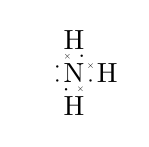
\begin{tikzpicture}[inner sep=1pt]
  \node (c){N};
  \foreach \x in {-1,0,1}
  {
    \node(h\x) at (90*\x:1.2em) {H};
    \draw[draw=none] (c)--(h\x)node[midway,sloped,above,inner sep=1pt]{\scalebox{0.35}{$\times$}}node[midway,sloped,below,inner sep=1pt]{\footnotesize$\cdot$};
  }
  \node(h2) at(180:1.2em){\phantom{H}};
  \draw[draw=none](c)--(h2)node[midway,above,inner sep=0pt]{\footnotesize$\cdot$}node[midway,below,inner sep=1pt]{\footnotesize$\cdot$};
\end{tikzpicture}\]
当 \ce{Cu^2+} 跟 \ce{NH3} 作用时，便以配位键形成了 \ce{[Cu(NH3)4]^2+}：
\[ \left[ 
  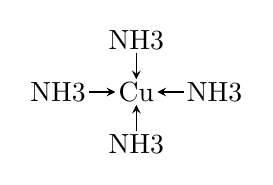
\begin{tikzpicture}[baseline,>=stealth,inner sep=1pt]
    \node (c) {\ce{Cu}};
    \node (u) at (0,0.5) [above]{\ce{NH3}};
    \node (d) at (0,-0.5)[below] {\ce{NH3}};
    \node (l) at (-0.6,0)[left] {\ce{NH3}};
    \node (r) at (0.6,0)[right] {\ce{NH3}};
    \draw[->](u)--(c);
    \draw[->](d)--(c);
    \draw[->](l)--(c);
    \draw[->](r)--(c);
  \end{tikzpicture}
 \right]^{2+}\]

过渡元素离子如 \ce{Fe^3+}、\ce{Fe^2+}、\ce{Cu^2+}、\ce{Ag+}、\ce{Hg^2+} 等都具有空轨道，因此都容易形成络合物，这是过渡元素的特性。
至于 \ce{F-}、\ce{Cl-}、\ce{CN-}、\ce{SCN-} 等阴离子或 \ce{H2O}、\ce{NH3} 等分子都有孤对电子，因而都可以成为配位体。
凡是可作配位体（或含有可作配位体的离子）的物质叫做\Concept{络合剂}。
常用的络合剂有氰化物、氟化物和氨等。

\begin{Reading}{络合物在水溶液里的电离平衡}
络合物的外界跟内界是以离子键结合的，因此，当络合物溶于水时，络合物会发生电离而形成外界和内界两种离子。同时，络离子在水里也会发生一定程度的电离。例如：
\begin{gather*} 
  \schemestart
  \ce{ [Cu(NH3)4]^2+} \arrow(.mid east--.mid west){<=>} \ce{Cu^2+} \+ \ce{4NH3  }
  \schemestop\\ 
  \schemestart
  \chemname{\ce{[Ag(NH3)2]+}}{\footnotesize 二氨合银离子（银氨络离子）}
  \arrow(.mid east--.mid west){<=>} \ce{Ag+} 
  \+ 
  \ce{2NH3}\schemestop\chemnameinit{}\\
  \schemestart
  \chemname{\ce{[Ag(CN)2]-}}{\footnotesize 二氰合银离子（银氰络离子）}
  \arrow(.mid east--.mid west){<=>} \ce{Ag+} 
  \+ 
  \ce{2CN-}\schemestop\chemnameinit{}
\end{gather*}

不同络离子电离程度的大小不同。
一般说来，配位体是 \ce{CN-} 的络离子的电离程度总是很小。
人们利用含氰络离子电离程度很小，即溶液里跟络离子达成平衡的金属离子浓度很小的特点，在电镀工艺中控制金属离子结合电子的速度，从而保证电镀的质量。
所以在电镀工业里配制电镀液时常使用氰化物作络合剂。
但是氰化物有剧毒，因此，现在电镀工业正在研究和使用别的无毒络合剂的无氰电镀工艺。
\end{Reading}


\subsection{络合物的应用}
络合物在自然界广泛存在，跟人类生活的关系很密切。
例如，在人和动物体内起着输送氧气作用的血红素，是 \ce{Fe^2+} 的络合物；在植物生长中起光合作用的叶绿素是含 \ce{Mg^2+} 的络合物。

络合物在工农业生产和科学技术方面的应用也很广泛，例如，在冶金、稀有金属的提取、电镀、照相术等方面都有应用，氰化提金法就是用于稀有金属提取的一个例子。
这个方法的原理是: 用稀的氰化钠溶液处理粉碎了的金矿石，通入空气，使金矿石中的金粒溶解，生成能溶于水的络合物 \ce{Na[Au(CN)2]}：
\[ \ce{4Au + 8NaCN + 2H2O + O2 \xlongequal{\quad} 4Na[Au(CN)2] + 4NaOH} \]
然后再用锌从溶液中把金置换出来：
\[ \ce{ 2Na[Au(CN)2] + Zn \xlongequal{\quad} Na2[Zn(CN)4] + 2Au v} \]

在照相底片和感光纸定影时，需要应用硫代硫酸钠溶液溶解掉未起反应的溴化银，这是一个络合反应，它的化学方程式如下：
\[ \ce{AgBr + 2Na2S2O3 \xlongequal{\quad} Na3[Ag(S2O3)2] + NaBr} \]

在化学实验里，还可以利用形成显色的络离子或络合物来鉴定离子。
例如，利用 \ce{SCN-} 跟 \ce{Fe^3+} 反应生成红色的硫氰合铁（\MyRoman{3}）离子 \ce{[Fe(SCN)]^2+}，可以判断溶液里 \ce{Fe^3+} 的存在。

\begin{Practice}[习题]
\begin{question}
  \item 现有硝酸二氨合银 \ce{[Ag(NH3)2]NO3} 和六氟合铝酸钠 \ce{Na3[AlF6]} 两种络合物，试指出它们各自的络离子，中心离子和它们的电荷数，配位体和配位数，络合物的内界和外界。
  \item 以 \ce{[Ag(NH3)2]+} 为例，说明中心离子跟配位体是怎样结合的。
  \item 氯化钠溶液和硝酸银溶液相遇，会生成白色的氯化银沉淀。往沉淀里加入氨水，沉淀又溶解了。怎样解释上述实验现象？写出反应的离子方程式。（提示: 参照课文里铜氨络离子的生成，银离子的配位数是 2。）
  \item 为什么无水硫酸铜的白色的晶体溶于水后成为浅蓝色溶液，在这个溶液里滴入少量氨水，溶液又变为深蓝色？
\end{question}
\end{Practice}


\section{铁}
\subsection{铁的性质}
铁在元素周期表里位于第四周期的第 \MyRoman{8} 族，是一种极为重要的过渡元素。
它有多种可变化合价，铁的化合物及其离子大多呈现颜色，并容易形成络合物。
铁原子的外围电子层排布是 $3d^64s^2$，最外层 $4s$ 轨道有两个电子，次外层 $3d$ 轨道的电子未充满。
在起化学反应的时候，铁原子容易失去两个 $4s$ 电子，也容易再失去一个 $3d$ 电子。
所以，铁通常显 $+2$ 价和 $+3$ 价。但是,由于 $+3$ 价的铁的 $3d$ 轨道为半充满稳定结构，因此 $+3$ 价的铁最稳定，其次是 $+2$ 价的铁。

\subsubsection{铁的物理性质}
纯净的铁是光亮的银白色金属，它的密度是 \qty{7.86}{g/cm^3}，熔点是 \qty{1535}{\celsius}，沸点是 \qty{2750}{\celsius}。
纯铁的抗蚀力相当强，但通常用的铁一般都含有碳和其它元素，因而使它的熔点显著降低，抗蚀力也减弱。
铁有延展性和导热性。铁也能导电，但是它的导电性比铜、铝都差。
铁能被磁体吸引。
在磁场的作用下，铁自身也能产生磁性。

\subsubsection{铁的化学性质}
铁是比较活泼的金属，在金属活动性顺序表里它列在氢的前面。

\paragraph{铁跟氧气和其它非金属的反应}\mbox{}\par
常温时，铁在干燥的空气里不易跟氧气起反应，但把铁放在氧气里灼烧，就会生成一种黑色的四氧化三铁。
\[ \ce{3Fe + 2O2 \xlongequal{\text{点燃}} Fe3O4} \]

加热时，铁也能跟其它非金属，如硫、氯气等发生反应，分别生成硫化亚铁和氯化铁
\begin{align*}
  \ce{Fe + S} &\xlongequal{\triangle} \ce{FeS}\\
  \ce{2Fe + 3Cl2} &\xlongequal{\triangle} \ce{2FeCl3}
\end{align*}

在铁跟硫的反应里，铁原子失去 2 个 $4s$ 电子变成 $+2$ 价的铁。
在铁跟氯气的反应里，铁原子不仅失去 2 个 $4s$ 电子，而且还失去 1 个 $3d$ 电子，变成 $+3$ 价的铁。
这是因为氯气是一种更强的氧化剂，它夺取电子的能力比硫强的缘故。

在高温下，铁还能跟碳、硅、磷等化合。
例如，铁跟碳能化合而生成一种灰色的、脆、硬而难熔的碳化铁（\ce{Fe3C}）。

\paragraph{铁跟水的反应}\mbox{}\par
红热的铁能跟水蒸气起反应，生成四氧化三铁和氢气。
\[ \ce{ 3Fe + 4H2O\,\text{（气）}\xlongequal{\text{高温}} Fe3O4 + 4H2 ^ }\]

在常温下，铁跟水不起反应。
但是，在水和空气里的氧气以及二氧化碳等的共同作用下，铁却很容易发生电化腐蚀。

此外，铁还能跟盐酸、稀硫酸和某些金属盐发生置换反应。
例如，铁跟盐酸或稀硫酸起反应，置换出氢气。
\[ \ce{ Fe + 2H+ = Fe^2+ +H2 ^} \]

铁跟比它活动性较弱的铜的盐溶液起反应，置换出金属铜。
\[ \ce{Fe + Cu^2+ = Fe^2+ + Cu} \]

\subsection{铁的化合物}
\subsubsection{铁的氧化物}
铁的氧化物有氧化亚铁（\ce{FeO}）、氧化铁（\ce{Fe2O3}）和四氧化三铁 （\ce{Fe3O4}）等。

氧化亚铁是一种黑色粉末，它不稳定，在空气里加热，即迅速被氧化成四氧化三铁。

氧化铁是一种红棕色粉末，俗称铁红，它可用作油漆的颜料等。

四氧化三铁是具有磁性的黑色晶体，俗称磁性氧化铁。
四氧化三铁是一种复杂的化合物，在四氧化三铁晶体里存在着铁的两种不同价态的离子，其中 $\frac13$ 是 \ce{Fe^2+}，$\frac23$ 是 \ce{Fe^3+}，因此，四氧化三铁可以看成是氧化亚铁跟氧化铁组成的化合物。

铁的氧化物都不溶于水，也不跟水起反应。

氧化亚铁和氧化铁都能跟酸起反应，分别生成亚铁盐和铁盐。
\begin{align*}
  \ce{ FeO + 2H+ } & = \ce{  Fe^2+ + H2O }\\ 
  \ce{ Fe2O3 + 6H+ } & = \ce{ 2Fe^3+ + 3H2O }
\end{align*}

\subsubsection{铁的氢氧化物}
跟氧化亚铁和氧化铁相对应的碱分别是氢氧化亚铁（\ce{Fe(OH)2}）和氢氧化铁（\ce{Fe(OH)3}）。这两种氢氧化物都可用相对应的可溶性盐跟碱溶液起反应而制得。
\begin{Experiment}
在试管里注入少量新制备的硫酸亚铁溶液，用胶头滴管吸取氢氧化钠溶液，将滴管端插入试管里溶液的液面下，再逐滴滴入氢氧化钠溶液，观察发生的现象。
\end{Experiment}
从实验可以看到，滴入氢氧化钠溶液后，开始的时候析出一种白色的絮状沉淀，这就是氢氧化亚铁。
\[ \ce{ Fe^2+ + 2OH- = Fe(OH)2 v }\]
但这白色絮状沉淀迅速变成灰绿色，最后变成红褐色。
这是因为氢氧化亚铁在空气里氧化成了氢氧化铁。
\[ \ce{ 4Fe(OH)2 + O2 + 2H2O \xlongequal{\quad} 4Fe(OH)3 v}\]
\begin{Experiment}
  在试管里注入少量氯化铁溶液，再逐滴滴入氢氧化钠溶液。观察发生的现象。
\end{Experiment}
从实验可以看到，滴入氢氧化钠溶液时，立即生成了红褐色的氢氧化铁沉淀。
\[ \ce{ Fe^3+ + 3OH- = Fe(OH)3 v}\]

加热氢氧化铁，它就失去水而生成红棕色的氧化铁粉末。
\[ \ce{ 2Fe(OH)3 \xlongequal{\triangle} Fe2O3 + 3H2O }\]

氢氧化亚铁和氢氧化铁都是不溶性碱，它们能跟酸反应，分别生成亚铁盐和铁盐。
\begin{align*}
  \ce{Fe(OH)2 + 2H+}  &= \ce{Fe^2+ + 2H2O}\\
  \ce{Fe(OH)3 + 3H+}  &= \ce{Fe^3+ + 3H2O}
\end{align*}

\subsubsection{铁化合物和亚铁化合物间的相互转变}
铁化合物遇较强的还原剂会还原成亚铁化合物。
例如，氯化铁溶液遇铁等还原剂，能被还原生成氯化亚铁。
\[ \ce{ 2Fe^3+ + Fe = 3Fe^2+} \]

亚铁化合物在较强的氧化剂的作用下会氧化成铁化合物。
例如，氯化亚铁溶液跟氯气起反应，立即被氧化成氯化铁。
\[ \ce{ 2Fe^2+ + Cl2 = 2Fe^3+ + 2Cl-} \]

从以上事实可以说明，\ce{Fe^2+} 和 \ce{Fe^3+} 在一定条件下是可以相互转变的。
\[\schemestart \ce{ Fe^2+ } \arrow{<=>[\footnotesize 氧化剂][\footnotesize 还原剂]} \ce{ Fe^3+ + e} \schemestop\]

\subsubsection{铁的络合物和 \ce{Fe^3+} 的检验}
铁有多种络合物，重要的有六氰合铁络合物，如六氰合铁（\MyRoman{2}）酸钾 \ce{K4[Fe(CN)6]}（也叫亚铁氰化钾，俗名黄血盐）、六氰合铁（\MyRoman{3}）酸钾 \ce{K3[Fe(CN)6]}（也叫铁氰化钾，俗名赤血盐），以及硫氰合铁（\MyRoman{3}）络离子 \ce{[Fe(SCN)]^2+}，等等。
\begin{Experiment}
在试管里注入少量氯化铁溶液，再滴入几滴 \ce{KSCN} 溶液。观察发生的现象。
\end{Experiment}

\begin{Experiment}
在试管里注入少量氯化铁溶液，滴入几滴稀盐酸，加入少量铁屑，轻轻振荡片刻，再滴入几滴 \ce{KSCN} 溶液。观察发生的现象。
\end{Experiment}

我们可以利用无色的 \ce{SCN-} 跟 \ce{Fe^3+} 反应，生成红色的络离子 \ce{[Fe(SCN)]^2+}\footnote{\ce{Fe^3+} 跟 \ce{SCN-} 可以生成配位数从 1 到 6 的络离子：\ce{[Fe(SCN)]^2+}、\ce{[Fe(SCN)2]+}……\ce{[Fe(SCN)6]^3-}。它们的水溶液都呈红色。}，来检验 \ce{Fe^3+} 的存在。但 \ce{Fe^2+} 跟 \ce{SCN-} 反应不显红色。
\[ \ce{ Fe^3+ + SCN- = [Fe(SCN)]^2+ }\]

\begin{Practice}[习题]
\begin{question}
  \item 写出铁跟下列物质起反应的化学方程式或离子方程式：
  \begin{tasks}(4)
    \task 氧气，
    \task 稀硫酸，
    \task 硫酸铜溶液，
    \task 水蒸气。
  \end{tasks}
  \item 为什么铁跟硫起反应生成的是硫化亚铁，而跟氯气起反应生成的却是氯化铁而不是氯化亚铁？为什么铁跟盐酸起反应生成的是氯化亚铁而不是氯化铁？
  \item 用化学方程式表明下列的变化：
  \[ 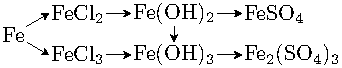
\includegraphics{pr1-3-3.pdf}\]
  \item 我们已知 \ce{Fe^2+} 跟 \ce{SCN-} 反应不显红色，但取实验室的 \ce{FeSO4} 试剂制成溶液后，滴加 \ce{KSCN} 溶液，常显淡红色,为什么？
  \item 氯气跟铁起反应能生成氯化铁。问用 \qty{260}{kg} 的氯气（设氯气的利用率为 96\%）跟足量的废铁屑起反应，能生成多少千克浓度为 42\% 的氯化铁溶液？
\end{question}
\end{Practice}

\section{炼铁和炼钢}
\subsection{铁的合金}
一般地说，含碳量在 2\%～4.3\% 的铁的合金叫做生铁。
生铁里除含碳外，还含有硅、锰以及少量的硫、磷等，它可铸不可锻。
根据生铁里碳存在的形态不同，又可分为炼钢生铁、铸造生铁和球墨铸铁等几种。
\begin{enumerate}
  \item 炼钢生铁\quad 碳在这种铁的合金里主要是以碳化铁（\ce{Fe3C}）的形态存在。这种生铁质硬而脆，难于加工，一般都用来炼钢，所以叫它炼钢生铁。由于它的断口呈白色，通常又叫白口铁。
  \item 铸造生铁\quad 碳在这种铁的合金里是以片状的石墨形态存在。由于石墨质软并有润滑作用，因而这种生铁具有良好的切削、耐磨和铸造性能等优点。但是，由于有片状石墨的存在，降低了它的抗拉强度，使它不能锻轧，只能用于制造各种铸件，如铸造机床床座、铁管等。因此，通常把这种生铁叫做铸造生铁（简称铸铁）。由于它的断口呈灰色，通常又叫灰口铁。
  \item 球墨铸铁\quad 把铸造生铁加热熔化，用镁合金或稀土合金等处理，就能使铁碳合金里的石墨从片状变为球状。这种球状石墨的形成使铸铁的机械性能大大地提高。球墨铸铁比普通铸铁好，它的某些性能接近于钢，而价格却比钢便宜得多。因此，它可以代替一部分钢材用于制造曲轴、齿轮、阀门等。
\end{enumerate}

此外，还有含硅、锰或其它元素量特别高的生铁，叫做合金生铁（或铁合金），如硅铁、锰铁，等等。铁合金是炼钢的原料之一，在炼钢时加入了某些合金，可以改善钢的性能。

含碳量一般在 0.03\%～2\% 的铁的合金叫做\Concept{钢}。钢坚硬,有韧性、弹性，可以锻打、压延，也可以铸造。

钢的分类方法很多，如果按化学成分分类，钢可以分为碳素钢和合金钢两大类。
\begin{enumerate}
  \item 碳素钢，就是普通钢。它所含的碳、硅、锰比生铁少得多，硫和磷的含量也比生铁低很多。根据含碳量的不同，碳素钢的性质也各不相同，含碳量越多的硬度越大，含碳量越低的韧性越强。工业上一般把含碳量低于 0.3\% 的叫做低碳钢；含碳量在 0.3\%～0.6\% 之间的叫做中碳钢；含量在 0.6\% 以上的叫做高碳钢。低碳钢和中碳钢用来制造机器零件、管子等，高碳钢用来制造刀具、量具和冲压模具等。
  \item 合金钢，也叫特种钢。在碳素钢里适量地加入一种或几种合金元素\footnote{经常加入钢里的合金元素有: 硅、锰、铬、镍、钨、钼、钒、钛、锆、 铝、铜、铌、硼、镧系元素等等。}，使钢的组织结构发生变化，从而使钢具有各种不同特殊性能，如强度、硬度大，可塑性、韧性好，耐磨，耐腐蚀，以及其它许多优良性能。例如，钨钢、锰钢硬度很大，可以制造金属加工工具、拖拉机履带和车轴等；锰硅钢韧性特别强，可以制造弹簧片、弹簧圈；钼钢能抗高温，可以制造飞机的曲轴、特别硬的工具等；钨铬钢的硬度大，韧性很强，可以做机床刀具和模具；镍铬钢抗蚀性强，不易氧化，是一种不锈钢，可以制造化工生产上用的耐酸塔、医疗器械、日常用具等。
\end{enumerate}

\subsection{炼铁}
铁是自然界里分布最广的金属元素之一，在地壳中的含量约占 5\% 左右,仅次于铝。
由于铁的化学性质比较活泼，所以分布在地壳中的铁都是以化合态存在，游离态的铁只能从陨石中得到。
我们把自然界里能用来炼铁的含铁矿物叫做铁矿石。

铁矿石的种类很多，重要的有磁铁矿石（主要成分是 \ce{Fe3O4}）、赤铁矿石（主要成分是 \ce{Fe2O3}）、褐铁矿石（主要成分是 \ce{2Fe2O3.3H2O}）和菱铁矿石（主要成分是 \ce{FeCO3}）等。
铁矿石里除含铁的化合物外，还含有脉石（主要成分是 \ce{SiO2}）和硫、 磷等杂质。

怎样把铁矿石炼成铁呢？它的主要反应原理可以用以下的实验加以说明。
\begin{Experiment}
  如\cref{fig:1-3} 的装置，在硬质玻璃管里放入少量红棕色的氧化铁粉末，通入一氧化碳，然后加热。观察发生的现象。
  \tcblower
  \begin{figurehere}
    \includegraphics{1-3.pdf}
    \caption{用一氧化碳还原氧化铁的实验装置}\label{fig:1-3}
  \end{figurehere}
\end{Experiment}
我们可以看到，玻璃管里的粉末由红棕色逐渐变黑。
这种黑色的粉末就是被还原出来的铁。
试管里澄清的石灰水变浑浊，证明有二氧化碳生成。

由此可知，氧化铁在加热时能被一氧化碳还原成铁，同时生成二氧化碳。
\[ \ce{ Fe2O3 + 3CO \xlongequal{\triangle} 2Fe + 3CO ^}\]

把铁矿石冶炼成铁是一个复杂的过程，但是它的主要反应原理，就是利用氧化—还原反应，在高温下，用还原剂（主要是一氧化碳）从铁矿石里把铁还原出来。

\medskip\noindent\begin{minipage}{0.45\linewidth}\parindent2em
炼铁一般是在高炉（\cref{fig:1-4}）里连续进行的。

高炉是由炉喉、炉身、炉腰、炉腹、炉缸等五部分组成，并有进料口、进风口、出铁口、出渣口和高炉煤气出口。

炼铁的主要原料是铁矿石、焦炭、石灰石和空气。

炼铁的时候，把铁矿石、焦炭和石灰石按一定比配成炉料，从炉顶进料口分批加入炉内，同时把预热过的空气从炉腹底部的进风口鼓入炉内。
因为热的气体由下上升，炉料由上下落，它们在炉内能够充分接触，使反应得以顺利进行，同时又能使炉料逐步预热，使热能得以充分利用。在进风口附近，焦炭遇热空气燃烧生成二氧化碳，并放出大量的热。
\end{minipage}\hfill
\begin{minipage}{0.53\linewidth}
  \begin{figurehere}
    \includegraphics{1-4.pdf}
  \caption{高炉和炉内的化学变化过程示意图}\label{fig:1-4}
\end{figurehere}
\end{minipage}

\[ \ce{ C + O2 \xlongequal{\quad} CO2 } + \text{热量} \]

二氧化碳气体上升，跟赤热的焦炭反应，生成一氧化碳。
\[ \ce{ CO2 + C \xlongequal{\quad} 2CO } - \text{热量} \]

一氧化碳气体上升，跟从炉顶不断装入并逐步下降的铁矿石接触。
在炉身中部，绝大部分铁的氧化物被一氧化碳还原成铁。
\[ \ce{ Fe2O3 + 3CO \xlongequal{\text{高温}} 2Fe + 3CO2 ^ }\]

在冶炼过程中，混在铁矿石里的锰、硅、硫、磷等元素也会被碳或一氧化碳从它们的化合物中还原出来。少量的碳、锰、硅、硫。磷等在高温下熔合在铁里，成为生铁。生铁的熔点（\qtyrange{1100}{1200}{\celsius}） 比纯铁的熔点（\qty{1535}{\celsius}）低得多。

铁矿石里除了铁的氧化物外，还含有难熔化的脉石，如果不把它们除去，就会影响生铁的冶炼。
加入的石灰石是作为熔剂，用来除去脉石的。
因为石灰石在高温下分解出的氧化钙，能跟脉石里的二氧化硅起反应而生成熔点较低的硅酸钙，从矿石里分离出来。
\begin{gather*}
  \ce{ CaCO3 \xlongequal{\text{高温}} CaO + CO2 ^} \\
  \ce{ CaO + SiO2 \xlongequal{\text{高温}} CaSiO2 }
\end{gather*}

硅酸钙是炉渣的主要成分。

从高炉里放出来的铁水可以直接用来炼钢，或铸成铁锭或铸件。
炉渣可以作为水泥、渣砖等的原料。
从炉顶放出的一氧化碳、二氧化碳和氮气等混和气体叫高炉煤气。
因其中含有大量灰尘和有害气体，必须经过净化处理，以防止污染环境。
除去尘粒后的高炉煤气里含有热值很高的一氧化碳，可作为气体燃料。

为了提高生产效率，现代化的高炉生产采取了一系列新技术，强化冶炼强度，提高风温，以降低焦比（每炼一吨生铁所需要的焦炭的公斤数），提高高炉的利用系数（每立方米高炉有效容积一昼夜生产生铁的吨数）等。

\subsection{炼钢}
钢在工农业生产和国防建设中的用途远远超过了生铁，因此，我们需要把大部分生铁冶炼成钢。

把生铁冶炼成钢的实质，就是适当地降低生铁里的含碳量，除去大部分硫、磷等有害杂质，调整钢里合金元素含量到规定范围之内。
炼钢的主要反应原理，也是利用氧化—还原反应，在高温下，用氧化剂把生铁里过多的碳和其它杂质氧化成为气体或炉渣除去。
因此，炼钢和炼铁虽然都是利用的氧化—还原反应，但是炼铁主要是用还原剂把铁从铁矿石里还原出来，而炼钢主要是用氧化剂把生铁里过多的碳和其它杂质氧化而除去。

炼钢时常用的氧化剂是空气、氧气或氧化铁。
当加入氧化剂后，由于生铁里最大量的物质是铁，所以铁首先被氧化，使部分铁变成了氧化亚铁，同时放出大量的热：
\[ \ce{ 2Fe + O2 \xlongequal{\quad} 2FeO} + \text{热量}\]

之后，生成的氧化亚铁再把铁水里的硅、锰、碳等依次氧化：
\begin{gather*}
  \ce{ Si + 2FeO \xlongequal{\quad} SiO2 + 2Fe} + \text{热量} \\ 
  \ce{ Mn + FeO \xlongequal{\quad} MnO + Fe} + \text{热量} \\ 
  \ce{ C + FeO \xlongequal{\quad} CO + Fe} - \text{热量} 
\end{gather*}

铁水里的一部分硅、锰、碳等元素也会被氧气直接氧化。

生成的一氧化碳气体，能从铁水里直接排出；生成的二氧化硅和氧化锰跟造渣材料生石灰相互作用成为炉渣排出。

生铁里的硫、磷这两种元素，在炼钢时必须尽可能除去。
造渣材料生石灰也能跟硫\footnote{铁水里的硫，主要以 \ce{FeS} 形态存在。}、磷起反应、使硫、磷变成硫化钙和磷酸钙等炉渣而除去。
它们的主要反应可用化学方程式表示如下：
\begin{align*}
  \ce{FeS + CaO} & \xlongequal{\text{高温}} \ce{ FeO + CaS }\\
  \ce{2P + 5FeO + 3CaO} & \xlongequal{\text{高温}} \ce{ 5Fe + Ca3(PO4)2 }
\end{align*}

含磷量较高的炉渣可以加工制成磷肥。
这种磷肥叫做钢渣磷肥。

当铁水里的碳、硫、磷的含量已降低到符合炼钢的要求时，就可以把生成的炉渣排出炉外。
这时的铁水已变成钢水。 
但在这种钢水里还含有少量的氧化亚铁，它的存在会使钢具有热脆性，需要加入适当的脱氧剂（即还原剂）使钢脱氧。
通常都用硅铁、锰铁或金属铝等脱氧剂来还原氧化亚铁，例如：
\[ \ce{ 2FeO + Si \xlongequal{\text{高温}} 2Fe + SiO2 }\]

生成的二氧化硅等大部分形成炉渣而除去，部分的硅。
锰等留在钢里以调整钢的成分。

目前，炼钢的方法主要有转炉、电炉和平炉三种。
在这里，我们只简单介绍现在被广泛采用的比较先进的氧气顶吹转炉炼钢法。

\medskip\noindent\begin{minipage}{0.62\linewidth}\parindent2em
氧气顶吹转炉炼钢设备，如\cref{fig:1-5} 所示。
按照配料要求，先把废钢等装入炉内，然后倒入铁水，并加入适量的造渣材料（如生石灰等）。
加料后，把氧气喷枪从炉顶插入炉内，吹入氧气（纯度大于 99\% 的高压氧气流），使它直接跟高温的铁水发生氧化反应，除去杂质。
用纯氧代替空气可以克服由于空气里的氮气的影响而使钢质变脆，以及氮气排出时带走热量的缺点。
在除去大部分硫、磷后，当钢水的成分和温度都达到要求时，即停止吹炼，提升喷枪，准备出钢。
出钢时使炉体倾斜，钢水从出钢口注入钢水包里，同时加入脱氧剂进行脱氧和调节成分。
钢水合格后，可以浇成钢的铸件或钢锭，钢锭可以再轧制成各种钢材。
\end{minipage}\hfill
\begin{minipage}{0.35\linewidth}
\begin{figurehere}
  \includegraphics{1-5.pdf}
  \caption{氧气顶吹转炉示意图}\label{fig:1-5}
\end{figurehere}
\end{minipage}\par\medskip

氧气顶吹转炉在炼钢过程中会产生大量棕色烟气，它的主要成分是氧化铁尘粒和高浓度的一氧化碳气体等。
因此，必须加以净化回收，综合利用，以防止污染环境。
从回收设备得到的氧化铁尘粒可以用来炼钢；一氧化碳可以作化工原料或燃料；烟气带出的热量可以副产水蒸气。
此外，炼钢时，生成的炉渣也可以用来做钢渣水泥，含磷量较高的炉渣，可加工成磷肥，等等。

氧气顶吹转炉炼钢法具有冶炼速度快、炼出的钢种较多、质量较好，以及建厂速度快、投资少等许多优点。
但在冶炼过程中都是氧化性气氛，去硫效率差，昂贵的合金元素也易被氧化而损耗，因而所炼钢种和质量就受到一定的限制。

\begin{Theorem}{讨论}
  炼铁和炼钢的主要反应原理有什么异同。
\end{Theorem}

\begin{Practice}[习题]
\begin{question}
  \item 生铁和钢在含碳量方面有什么不同？
  \item 写出高炉炼铁主要反应的化学方程式。指出哪些是氧化—还原反应，哪些不是。在氧化—还原反应里，指出什么物质是氧化剂，什么物质是还原剂。
  \item 在含杂质 30\% 的磁铁矿石和含杂质 20\% 的赤铁矿石里，含铁的百分率哪个高？
  \item 某大型高炉年产生铁 \qty{400e4}{t}（设生铁里含铁 96\%，在冶炼中铁的总损耗不计），问需要含铁 50\% 的赤铁矿石多少万吨？
  \item \qty{100}{t} 含 \ce{Fe2O3} 85\% 的铁矿石可炼出含铁 96\% 的生铁多少吨？
  \item 在炼钢开始和熔炼完毕时，都有下列反应进行：
  \begin{gather*}
    \ce{ 2FeO + Si \xlongequal{\text{高温}} 2Fe + SiO2 } \\
    \ce{ FeO + Mn \xlongequal{\text{高温}} Fe + MnO }
  \end{gather*}
  试说明它们对炼钢的作用有什么不同。
\end{question}
\end{Practice}


\section{铜}
\subsection{铜的性质和用途}
\subsubsection{铜的性质}
铜属于元素周期表的 \MyRoman{1}B 族，原子的外围电子层排布是 $3d^{10}4s^1$，$d$ 轨道已经充满。铜跟 \MyRoman{1}A 族的钾处于同一周期，电子层数和最外层电子数都相同，但次外层电子排布不同，铜是 18 个电子，钾是 8 个电子，铜的核电荷数比钾多，原子半径比钾小，核对外层电子的吸引力和电离能都比钾大，失去电子远不如钾容易，因此化学性质也就远不如钾活泼。由于 $3d$ 轨道跟 $4s$ 轨道能级相近，$d$ 电子也可以参加成键，因此铜通常有 $+1$、$+2$ 两种价态,但以 $+2$ 价为主。

铜是具有紫红色光泽的金属，熔点是 \qty{1083}{\celsius}，密度是 \qty{8.92}{g/cm^3}，质软，有很好的导电、导热性能、延展性也很好。
铜还有较好的耐腐蚀能力，在干燥的空气里很稳定，不跟稀盐酸和稀硫酸起反应。
但铜在潮湿的空气里表面上能生成一层绿色的碱式碳酸铜 （\ce{Cu2(OH)2CO3}），俗称铜绿。
这个反应可以简单表示如下：
\[ \ce{2Cu + O2 + H2O + CO2 \xlongequal{\quad} Cu2(OH)2CO3} \]

高温下铜能氧化。把铜放在空气里加热到 \qty{300}{\celsius} 时，铜的表面就生成一层黑色的氧化铜。
\[ \ce{ 2Cu + O2 \xlongequal{\triangle} 2CuO }\]

高温时铜容易跟硫、卤素等化合，但不跟氮气化合。

铜能跟氧化性酸如浓硝酸、稀硝酸和热的浓硫酸起反应，生成 $+2$ 价铜盐和相应的氮或硫的氧化物。
实验室里常利用这种方法来制备这些氮或硫的氧化物。

\subsubsection{铜的用途}
人类使用铜和它的合金具有悠久的历史。
我国劳动人民早在三千多年前的商代就已经会制造青铜器。
从发掘的出土文物中我们知道，商代已经使用青铜制造的农具、武器和祭祀用品。
例如巨大的司母戊大鼎重达 \qty{875}{kg}，制作精美，表现出我国劳动人民很早就已经掌握了高超的冶炼和铸造技术。

在现代，铜仍然是一种很重要的金属，在世界上它的产量仅次于铁和铝，占第三位。

由于铜的导电性良好，所以铜广泛用于电器工业，制作电线、电缆和各种电器设备。
全世界每年消耗于电器工业的铜占铜的总产量的一半。
铜还可以制成各种合金，如黄铜（\ce{Cu}--\ce{Zn} 合金）、青铜（\ce{Cu}--\ce{Sn} 合金）等。
铜和铜的合金在机械和仪器、仪表工业里用来制造各种零件；在国防工业里用来制造枪弹、炮弹；在化学工业里用来制造热交换器、深度冷冻装置等。

\subsection{铜的化合物}
常见的铜的氧化物有氧化亚铜（\ce{Cu2O}）和氧化铜（\ce{CuO}）两种。
氧化亚铜呈红色，氧化铜呈黑色。
把氧化铜加热到 \qty{800}{\celsius}，氧化铜就开始分解为氧化亚铜和氧气。
\[ \ce{ 4CuO \xlongequal{\text{高温}} 2Cu2O + O2 ^} \]
氧化铜可作为制造铜盐的原料，氧化亚铜可作为制造玻璃、搪瓷的红色颜料。

$+2$ 价铜盐溶液跟适量的碱溶液起反应，生成蓝色的氢氧化铜沉淀。
把所得的氢氧化铜沉淀溶于氨水中，即生成络合物氢氧化铜氨。
\[ \ce{ Cu(OH)2 +4NH3.H2O \xlongequal{\quad} [Cu(NH3)4](OH)2 +4H2O } \]
氢氧化铜氨能溶解纤维素，加酸后纤维素又能沉淀出来。
利用这个特点可以制造一种人造丝。

五水硫酸铜 \ce{CuSO4.5H2O} 俗名胆矾，用于配制电解法精炼铜和电镀铜的电解液。
也可跟石灰乳混和配成波尔多液，作为防治植物病害的农药。

\subsection{铜在自然界的存在}
铜在地壳里的含量约占地壳质量的万分之一。
自然界里天然铜很少，大都以化合物的形式存在，矿藏有黄铜矿（\ce{CuFeS2}）、辉铜矿（\ce{Cu2S}）、孔雀石（\ce{Cu2(OH)2CO3}）、赤铜矿（\ce{Cu2O}）等。

\subsection{铜的电解法精炼}
电器工业使用的铜对纯度要求很高，而从矿石经过一系列处理炼得的铜还含有 0.5\%～1.5\% 的各种杂质（锌、铁、镍、银、金等），导电性能不好，不符合电器工业的要求，需要用电解法再进行精炼。

电解时，用含杂质的铜做阳极，用纯铜薄片做阴极，以硫酸铜溶液作电解液，通以一定电压的直流电。
这时，两极发生如下反应：

在阳极 \quad\ce{ Cu - 2e = Cu^2+ }

在阴极 \quad\ce{ Cu^2+ + 2e = Cu }

当含杂质的铜在阳极不断溶解，位于金属活动性顺序铜以前的杂质元素如锌、铁、镍等，虽然也同时失去电子，如：
\[ \ce{ Zn - 2e = Zn^2+ } \quad \ce{ Ni - 2e = Ni^2+ } \]
但是它们的阳离子比 \ce{Cu^2+} 难以还原，所以它们不在阴极获得电子，只是溶解在电解液里。
而位于金属活动性顺序铜之后的银、金等金属杂质，因为给出电子的能力比铜弱，所以不在阳极失去电子，而是以金属单质的形式沉积在电解槽底，叫做阳极泥。
这样，在阴极就得到了纯铜，通常叫它电解铜（纯度可达 99.99\%）。
把阳极泥加以处理，可以得到金、银等贵重金属。

\subsection{用纸上层析法分离铜离子和铁离子}
\begin{Experiment}*[righthand ratio=0.3]
装置如\cref{fig:1-6} 所示。 取一条滤纸，用铅笔在离末端约 \qty{2}{cm} 处画 $\times$ 作记号，在记号上用毛细管滴一小滴饱和的 \ce{FeCl3} 和 \ce{CuSO4} 混和溶液作为试样，晾干再滴，共滴三遍，要求试样留下的斑点直径最好保持在 \qty{0.5}{cm} 以内。试样滴好后把滤纸固定在橡皮塞上。

  大试管里盛有丙酮和 $6N$ 盐酸（按体积比 $9:1$）混和而组成的溶剂。按\cref{fig:1-6} 把滤纸条末端浸入溶剂，但不能使试样斑点接触溶剂。塞上橡皮塞，静置。等到溶剂已扩散到滤纸上端时，就可取出滤纸，放在浓氨水瓶口，用氨气熏，观察发生的现象。
  \tcblower
  \begin{figurehere}
    \includegraphics{1-6.pdf}
    \caption{纸上层析}\label{fig:1-6}
  \end{figurehere}
\end{Experiment}
从实验可以看到，滤纸上端出现红棕色，红棕色的下方出现蓝色。
红棕色是 \ce{Fe^3+} 跟氨、水分作用生成的 \ce{Fe(OH)3} 的颜色；蓝色是 \ce{Cu^2+} 跟氨作用生成的铜氨络离子 \ce{[Cu(NH3)4]^2+} 的颜色。
这说明混和物中的 \ce{Cu^2+} 和 \ce{Fe^3+} 已经初步分开了。

混和物里的 \ce{Cu^2+} 和 \ce{Fe^3+} 为什么能被分离？原来 \ce{Cu^2+} 和 \ce{Fe^3+} 在滤纸上的扩散速度不相同。
\ce{Fe^3+} 扩散得快些，\ce{Cu^2+} 扩散得慢些，经过一段时间，它们相对富集的区域就分开了，从而达到了分离的目的。

在这个实验里，用氨气熏是为了显色，因此 \ce{NH3} 是显色剂。

象上述用滤纸和溶剂来使混和物分离的方法，叫做纸上层析。
应用纸上层析可以把性质相似的、难于分离的微量物质的混和物分离成各种成分，然后进行鉴别。
纸上层析使用的仪器简单，操作比较容易。
因此，它广泛地应用于中草药、 染料、色素和蛋白质等物质的分离和鉴别上。

\begin{Practice}[习题]
\begin{question}
  \item 铜原子和钾原子的电子层数和最外层电子数都相同，为什么铜的化学性质不如钾活泼？
  \item 为什么铜在电器工业里有广泛的应用？
  \item 写出下列各步反应的化学方程式：
  \[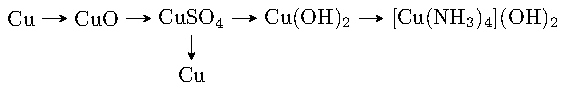
\includegraphics{pr1-5-3.pdf}\]
  \item 根据铜的电解精炼原理，回答下列问题：
  \begin{tasks}[label=(\arabic*)]
    \task 为什么用纯铜作阴极？
    \task 为什么用含杂质的铜作阳极？
    \task 电解液为什么要用铜盐？
    \task 阳极逐渐溶解以后，所含银、金等杂质为什么会沉积在电解槽底形成阳极泥？
    \task 杂质锌、铁、镍等也能失去电子变成阳离子进入溶液，但是它们为什么不在阴极析出？
  \end{tasks}
  \item 把 \ce{Cu} 跟 \ce{Fe}、\ce{Zn} 跟 \ce{Ag} 两组金属片分别放在盛有稀硫酸的烧杯里组成两组原电池，判别哪些金属是原电池的正极，哪些金属是原电极的负极，并写出在两极的反应。
\end{question}
\end{Practice}


\section{钛}
\subsection{钛的性质和用途}
\subsubsection{钛的性质}
钛位于元素周期表第四周期 \MyRoman{4}B 族，原子的外围电子层排布是 $3d^24s^2$。它在化学反应里不仅能失去 2 个 $4s$ 电子，呈 $+2$ 价，也能再失去 1 个或 2 个 $3d$ 电子，呈 $+3$ 价或 $+4$ 价，其中 $+4$ 价的化合物最稳定。这是由于呈 $+4$ 价时 $d$ 轨道全空，比呈 $+3$ 价、$+2$ 价时 $d$ 轨道分别有 1 个、2 个电子的电子层结构更为稳定的缘故。

钛的外观似钢，具有银灰色光泽，熔点是 \qty{1660}{\celsius}。
钛有一些非常可贵的性质，就是它的密度小，只有 \qty{4.5}{g/cm^3}，但是强度大。
我们知道，铝虽轻（密度 \qty{2.7}{g/cm^3}），但强度差；钢强度虽大，但太重（密度 \qty{7.9}{g/cm^3} 左右）。
所以，钛在密度和强度上兼有铝和钢两者的优点。
钛合金在 \qty{540}{\celsius} 高温和很低的温度（零下一百多度）下都能保持良好的机械性能，这是一种很可贵的性质。

钛有良好的抗腐蚀性能。
在通常情况下，钛很不活泼，在空气里加热到 \qtyrange{500}{600}{\celsius} 时，钛还是稳定的。
这是由于它的表面上生成了一层钝态的氧化物薄膜，阻止了它继续发生化学反应。

常温下，钛不被稀盐酸、稀硫酸、硝酸或稀碱液腐蚀，但能被氢氟酸、热的浓盐酸、浓硫酸和浓磷酸等腐蚀。

钛对潮湿的氯气和海水的耐蚀力特别强。

钛在高温下容易跟氧、硫、卤素、氮、碳等起反应，如在高温时，会在氧气流里燃烧，生成二氧化钛。
\[ \ce{ Ti + O2 \xlongequal{\text{高温}} TiO2 }\]
在高温下跟氯气起反应，生成四氯化钛。
\[ \ce{ Ti + 2Cl2 \xlongequal{\text{高温}} TiCl4 }\]

\subsubsection{钛的用途}
由于钛具有密度小、机械强度大、耐高温、耐腐蚀等优良性能，因此，钛和钛合金在航空工业、造船工业和化学工业等方面有着日益广泛的应用。

钛和钛合金在航空工业里主要是用来制作喷气发动机和飞机机体。
我们知道，减轻飞机、火箭、宇宙飞船的重量，能够大大节约燃料，提高飞行速度和扩大航程。
因此，用密度小的钛和钛合金代替密度大的钢材是很有利的。
另外，随着飞行速度的加快，由于同空气摩擦加剧，机体温度会迅速升高。
在那种情况下，铝会软化变形。
而用钛做的机体却能承受这种高温而不降低机械强度。
在造船工业上用钛合金制造海轮、舰艇的外壳及其它设备，既能减轻海水的腐蚀，又能减轻自身的重量，对于提高航速、增大载重量都有利。
在化学工业上，钛及其合金可以制作反应器、蒸馏塔、泵和阀门等设备。
防腐蚀效果比不锈钢好。
在冶金工业方面，可以利用加入钛来制造多种合金钢，如不锈钢、耐热钢等。

\subsection{钛的冶炼}
钛在地壳中蕴藏丰富，比常见的锌、铅、铜等金属的蕴藏量大得多，但分布很分散。
用于冶炼钛的矿物主要有钛铁矿（\ce{FeTiO3}）、金红石（\ce{TiO2}）等。我国有丰富的钛铁矿。

钛虽有优良的性能，但目前它还没有得到广泛的应用，原因是钛的冶炼相当困难。

钛的熔点很高，必须在高温下才能冶炼。
但钛在高温时化学性质活泼，容易跟氧、氮、碳等化合，形成杂质。
混有杂质的钛机械性能不好，发脆，抗蚀能力也大大减弱了。

现在冶炼钛的方法是，先把钛矿石经过一系列处理，转变成四氯化钛，再把四氯化钛用镁或钠还原，生成海绵状钛。
\[ \ce{ TiCl4 + 2Mg \xlongequal{\text{高温}} Ti + 2MgCl2 } \]
所得海绵状钛不能直接使用，还要在真空电弧炉里熔铸成钛锭，并经进一步加工才能得到可以使用的各种型材。

\section*{内容提要}
\addcontentsline{toc}{section}{内容提要}\setcounter{subsection}{0}
\subsection*{一、过渡元素}
\begin{enumerate}[1.]
  \item 过渡元素原子的电子层排布的特征是：最外层都有 \numrange{1}{2} 个 $s$ 电子（\ce{Pd} 除外）。除镧系、锕系元素外，随着原子序数的递增，新增加的电子大都填充在次外层的 $d$ 轨道上。镧系和锕系元素增加的电子主要填充在倒数第三层的 $f$ 轨道上。
  \item 过渡元素的通性
  \begin{itemize}
    \item 全是金属
    \item 常有多种可变化合价
    \item 化合物往往有颜色
    \item 易形成络合物
  \end{itemize}
\end{enumerate}

\subsection*{二、络合物}
\begin{enumerate}[1.]
  \item 由一种离子跟一种分子，或由一种离子跟另一种离子所形成的一类复杂离子，叫做络离子。含有络离子的化合物，属于络合物。
  \item 络合物的组成如下（以硫酸铜氨为例）：
  \[\begin{tikzpicture}[inner sep=0pt]
    \node (O) {[};
    \node (Cu) at(O.east)[right] {\ce{Cu}};
    \node (NH) at(Cu.east)[right] {\ce{(NH3)4}};
    \node (C)at(NH.east)[right]{]};
    \node (SO4)at(C.east)[right]{\ce{SO4}};
    \node at (SO4.north)[above=2pt]{\footnotesize 外界};
    \node at (NH.north)[above=2pt]{\footnotesize 内界};
    \draw (Cu)--++(-135:0.8)node[below]{\footnotesize 中心离子};
    \draw (NH)--++(-90:0.5657)node[below]{\footnotesize 配位体};
    \draw (NH.south east)--++(-45:0.47)node[below]{\footnotesize 配位数};
  \end{tikzpicture}\]
  \item 络合物内界和外界之间以离子键相结合。中心离子和配位体之间以配位键相结合。在形成配位键时，中心离子提供空轨道，配位体提供孤对电子。
  \item 络合物在工农业生产和科学技术上有广泛的用途，如用于提取稀有元素、电镀、照相术和离子鉴定等。
\end{enumerate}

\subsection*{三、铁}
铁在元素周期表里位于第四周期的第 \MyRoman{8} 族，是一种极为重要的过渡元素。
它的外围电子层排布是 $3d^64s^2$。
铁通常有 $+2$、$+3$ 两种价态的化合物，但以 $+3$ 价的较稳定。
它的化合物及其离子大都呈现颜色。
铁容易形成络合物。

铁在一定条件下，能跟氧气及其它非金属、酸、盐和水等起反应。

\ce{Fe^2+} 和 \ce{Fe^3+} 在一定条件下可以相互转变。
\[\schemestart \ce{Fe^2+} \arrow{<=>[\footnotesize 氧化剂][\footnotesize 还原剂]} \ce{Fe^3+ + e} \schemestop\]

\ce{Fe^3+} 的检验：\ce{Fe^3+} 跟 \ce{SCN-} 反应生成红色的 
\[\ce{[Fe(SCN)]^2+}\]

\subsection*{四、炼铁和炼钢}
\begin{enumerate}[1.]
  \item 铁的合金——生铁和钢
  
  \begin{tablehere}
    \begin{tblr}{colspec={X[c]X[2,c]X[c]X[2,c]X[2,c]},hline{2}=0.8pt}
     类别 & 含碳量 & 含杂质 & 机械行能 & 机械加工 \\
     生铁 & 2\%～4.3\% & 多 & 硬而脆 & 可铸不可锻 \\
     钢 & 0.03\%～2\% & 少 & 硬而韧，有弹性 & 可铸可锻 \\
    \end{tblr}
  \end{tablehere}
  \item 炼铁
  
  反应原理\quad 主要是用还原剂从铁矿石里把铁还原出来。
  \item 炼钢
  
  反应原理\quad 主要是用氧化剂把生铁里过多的碳及其它杂质氧化而除去。
\end{enumerate}

\subsection*{五、铜}
\begin{enumerate}[1.]
  \item 铜属于元素周期表的 \MyRoman{1}B 族，原子的外围电子层排布是 $3d^{10}4s^1$。铜通常有 $+1$、$+2$ 两种价态，但以 $+2$ 价为主。
  \item 铜有较好的耐腐蚀能力，在干燥的空气里很稳定，但在高温下容易跟氧、硫、卤素等化合。铜能被氧化性酸所氧化。
  \item 铜是一种很重要的金属，它有良好的导电、导热和延展性，广泛用于电器工业、国防工业和国民经济的其它部门。
\end{enumerate}

\subsection*{六、冶炼金属的一般方法}
\begin{enumerate}[1.]
  \item 使用还原剂法\quad 常用的还原剂有下列几种：
  \begin{enumerate}[(1)]
    \item 用一氧化碳或炭作还原剂。例如：
    \[ \ce{ Fe2O3 + 3CO \xlongequal{\text{高温}} 2Fe + 3CO2 ^} \]
    \item 用氢气作还原剂。例如：
    \[ \ce{ WO3 + 3H2 \xlongequal{\text{高温}} W + 3H2O }\]
    \item 用比较活泼的金属作还原剂。常用的还原剂有铝、钠、镁、钙等，例如：
    \[ \ce{ Cr2O3 + 2Al \xlongequal{\quad} 2Cr + Al2O3 } \]
  \end{enumerate}
  \item 电解法\quad 例如：
  \[ \ce{ 2Al2O3 \xlongequal{\text{电解}} 4Al + 3O2 ^ } \]
\end{enumerate}



\begin{Review}
\begin{question}
  \item 在下列过渡元素中，\CJKunderline[hidden]{\hspace{1em}F\hspace{1em}}元素具有最高的化合价。
  \begin{tasks}[label=\Alph*.](4)
    \task \ce{Cu}
    \task \ce{Zn}
    \task \ce{Fe}
    \task \ce{Ni}
    \task \ce{Cr}
    \task \ce{Mn}
    \task \ce{V}
    \task \ce{Ti}
  \end{tasks}
  \item 在氯化铁溶液里加入硫氰化钾溶液，立即出现红色。如果把硫氰化钾溶液加入铁氰化钾溶液，是否也显红色？说明理由。
  \item 某化合物的组成为 \ce{CoCl3.4NH3}，它 \qty{1}{mol} 跟过量 \ce{AgNO3} 反应，生成 \qty{1}{mol} \ce{AgCl}；向此化合物中加 \ce{H2SO4}，并不生成 \ce{(NH4)2SO4}。写出此化合物的化学式，指出它的内界和外界。
  \item 用铜、氧气、盐酸和氢氧化钠怎样制备氢氧化铜？用化学方程式表示。
  \item 现有 \qty{300}{mg} 的铜银合金，溶于硝酸后加水稀释，然后用了 $0.1N$ \ce{NaCl} 溶液 \qty{24}{ml}，恰好把溶液里的全部银离子沉淀。试写出有关反应的化学方程式，并求出合金里铜和银的百分组成。
  \item 利用含 30\% 硫酸的废液 \qty{2}{t} 跟足量的铁屑起反应，可生产出绿矾（\ce{FeSO4.7H2O}）多少吨？
  \item 在盛 \ce{FeCl2} 溶液的试管里，通入足量的氯气；在盛 \ce{FeCl3} 溶液的试管里，通入足量的硫化氢。然后向两个试管里分别加入几滴硫氰化钾溶液，各出现什么现象？分别写出有关反应的化学方程式和离子方程式。
  \item 用含 80\% 三氧化二铁的赤铁矿石作原料，生产 \qty{50}{t} 含 4\% 杂质的生铁，需要多少吨这种矿石？
  \item 炼铁时为什么要加入石灰石？写出有关的化学方程式。冶炼 \qty{1}{t} 含 15\% \ce{SiO2} 的铁矿石，至少要多少千克含 92\% \ce{CaCO3} 的石灰石才能把 \ce{SiO2} 全部除去？
  \item 取钢样 \qty{5}{g} 放在氧气流里灼烧，得到 \qty{0.0925}{g} 二氧化碳。求钢样里碳的百分含量。
\end{question}
\end{Review} % ok
\chapter{烃}
\section{有机物}
在日常生活和工农业生产里，人们从动物、植物等生物体中取得糖类、淀粉、蛋白质、油脂、纤维素和染料等等多种多样的化合物作为吃、穿、用等方面的必需品，已经有非常悠久的历史。
由于在那时这类化合物只能从动、植物等有机体中取得，因此人们就把这类化合物称为有机化合物。

从十九世纪二十年代开始，人们用非生物体内取得的物质先后合成了许多有机化合物，如尿素等。这样，就打破了只能从有机体取得有机化合物的限制。
现在，人们不但能够合成自然界里已有的许多种有机化合物，而且能够合成自然界里原来没有的多种多样性质良好的有机化合物，如合成树脂、合成橡胶、合成纤维和许多药物、染料等等。
因此“有机化合物”这个名称已失去了历史上原来的意义，只是因为大家习用这个名称，所以一直沿用着。

现在，我们所说的有机化合物，简称有机物，指的是含碳元素的化合物。
而把研究有机物的化学，叫做有机化学。
组成有机物的元素，除主要的碳外，通常还有氢、氧、氮、硫、卤素、磷等。
无机化合物，简称无机物\footnote{无机物里也包括单质。}，一般指的是组成里不含碳元素的物质。
我们过去已学过的很多化合物如水、食盐、氨、硫酸等等都是无机物。
而象一氧化碳、二氧化碳、碳酸盐等少数物质，虽然含有碳元素，但它们的组成和性质跟无机物很相近，一向把它们作为无机物。

有机物种类繁多，目前从自然界发现的和人工合成的有机物已达数百万种，而无机物却只有十来万种。
这是由于碳元素的原子的外层有四个价电子，可以跟其它原子形成四个共价键，而且更为突出的是碳原子跟碳原子之间能以比较稳定的共价键相结合，形成长的碳链。

一般说来，有机物具有以下主要特点。

大多数有机物难溶于水，易溶于汽油、酒精、苯等有机溶剂。
我们知道，许多无机物是易溶于水的。

绝大多数有机物受热容易分解，而且容易燃烧，而绝大多数无机物是不易燃烧的。

绝大多数有机物是非电解质，不易导电，熔点低。

有机物所起的化学反应比较复杂，一般比较慢，有的需要几小时甚至几天或更长时间才能完成，并且还常伴有副反应发生。
所以许多有机化学反应常常需要加热或应用催化剂以促进反应的进行。
这跟许多瞬时就可以完成的无机物的反应显然是不同的。

上面提到的有机化合物的许多物理性质和化学性质的特点，也是跟有机物的结构密切相关的。
大多数有机物分子里的碳原子跟其它原子经常是以共价键相结合，同时这些分子聚集时，又是分子晶体。
我们学习过的无机物许多是以离子键结合的，并形成离子晶体。
这些结构上的不同，就会在有机物的物理性质和化学性质方面表现出来。
当然严格来讲，有机物和无机物在性质上的区别也并不是绝对的。

由于有机物对发展国民经济和提高人民生活水平都具有重要意义，在近代，生产有机物的各种工业就越来越迅速地得到了发展。

有机化学早已从研究和利用天然有机物发展到大量用人工的方法制造（合成）新的有机物了。

有机化学在农业、能源、材料等科学技术研究领域里占有极为重要的地位。
有机化学也是研究跟生命有关的生物化学以及分子生物学的基础之一。

因此，学好有机化学，对于今后参加祖国的四个现代化建设是必要的。

\begin{Practice}[习题]
\begin{question}
  \item 什么叫有机物？组成有机物的元素主要的有哪几种？
  \item 简述有机物的特点。
\end{question}
\end{Practice}

\section{甲烷}
有机化合物里，有一大类物质是仅由碳和氢两种元素组成的,这类物质的总称叫烃\footnote{烃音\pinyin{ting1}。}，也叫碳氢化合物。
甲烷是烃类里分子组成最简单的物质。
\subsection{甲烷在自然界里的存在}
甲烷是没有颜色、没有气味的气体。
它的密度（在标准状况下）是 \qty{0.717}{g/L}，大约是空气密度的一半。
它极难溶解于水，很容易燃烧。

甲烷又叫沼气，也叫坑气。
这是因为池沼的底部和煤矿的坑道所产生的气体主要成分是甲烷的缘故。
这些甲烷都是在隔绝空气的情况下，由植物残体经过某些微生物发酵的作用而生成的。
此外，在有些地方的地下深处蕴藏着大量叫做天然气的可燃性气体，它的主要成分也是甲烷（按体积计，天然气里一般约含有甲烷  80\%～90\%，有的高达 98\%）。

沼气对于解决我国农村的能源问题，改善农村环境卫生，提高肥料质量等方面都有重要的意义。
近年来我国农村沼气的发展很快。

\subsection{甲烷分子的组成和结构}
甲烷由碳和氢两种元素组成。
根据标准状况下已测得甲烷气体的密度，我们可以计算出甲烷的摩尔质量约等于：
\[ \qty{0.717}{g/L} \times \qty{22.4}{L/mol} = \qty{16}{g/mol}\]

通过对甲烷气体进行的定量的测定，可以知道，甲烷里碳的百分含量是 75\%，氢的百分含量是 25\%。我们可以得出：

\qty{1}{mol} 甲烷分子里的含碳量约等于 $\qty{1}{mol} \times \qty{16}{g/mol}\times 75\%=\qty{12}{g}$。\qty{1}{mol} 碳原子的质量是 \qty{12}{g}，所以，\qty{1}{mol} 甲烷分子含 \qty{1}{mol} 碳原子。

\qty{1}{mol} 甲烷分子里的含氢量约等于 $\qty{1}{mol} \times \qty{16}{g/mol}\times 25\%=\qty{4}{g}$。\qty{1}{mol} 氢原子的质量是 \qty{1}{g}，所以，\qty{1}{mol} 甲烷分子含 \qty{4}{mol} 氢原子。

因此，甲烷的化学式是：\ce{CH4}。

那么，在甲烷分子里，1 个碳原子和 4 个氢原子是怎样结合的呢？要说明这个问题，让我们回忆碳原子核外电子排布的情况。碳原子的电子排布式是：$1s^22s^22p^2$，它的轨道表示式是：
\begin{figurehere}
  \includegraphics{2-a.pdf}
\end{figurehere}
它说明在碳原子的 4 个价电子里有两个 $2s$ 电子、两个 $2p$ 电子。
当碳原子参加化学反应时，1 个 $2s$ 电子在反应过程里吸收一定的能量，被激发到 $2p$ 轨道，这可表示如下：
\begin{figurehere}
  \includegraphics{2-b.pdf}
\end{figurehere}
这时,碳原子的未成对电子就是 1 个 $2s$ 电子和 3 个 $2p$ 电子。
因此，碳显示 4 价，它能跟 4 个氢原子形成 4 个共价键。
如果以 $\cdot$ 表示碳原子的价电子，以 $\scriptstyle\times$ 表示氢原子的价电子，甲烷的电子式可以写作：
\begin{figurehere}
  \includegraphics{2-c.pdf}
\end{figurehere}
在化学上常用一条短线来代表一对共用电子。
因此可以用下式来表示甲烷分子的结构：
\[ \chemfig{H-C(-[:90]H)(-[:-90]H)-H}\]

这种用短线来代表一对共用电子的图式叫做\Concept{结构式}。

甲烷的结构式虽然可以初步说明碳原子跟氢原子间的结合情况，但是并不能够说明分子里各原子在空间分布的实际情况。
经过大量的科学实验证明，甲烷分子里的一个碳原子和四个氢原子不在同一个平面上，而是形成了一个正四面体的立体结构。
碳原子位于正四面体的中心，而四个氢原子分别位于正四面体的四个顶点上。
碳原子的四个价键之间的夹角（键角）彼此相等，都是 \ang{109;28;}。
四个碳氢键的键长都是 \qty{1.09e-10}{m}。
经测定，\ce{C-H} 键的键能是 \qty{98.8}{kCal/mol}。
\cref{fig:2-1} 是甲烷分子结构的示意图，它可以表示分子里各原子的相对位置。
\cref{fig:2-2a} 是甲烷分子的一种模型，黑球代表碳原子，白球代表氢原子，短棍代表价键。这种模型叫做球棍模型。
\cref{fig:2-2b} 是甲烷分子的另一种模型，叫做比例模型。它用黑球和白球的体积比，来大体上表示碳氢两种原子的体积比。
\begin{figure}
  \begin{minipage}[b]{0.4\linewidth}\centering
    \includegraphics{2-1.pdf}
    \caption{甲烷分子结构的示意图}\label{fig:2-1}
  \end{minipage}%
  \begin{minipage}[b]{0.6\linewidth}
    \nextfloat
    \begin{subfigure}{0.48\linewidth}\centering
      \includegraphics{2-2a.pdf}
      \caption{球棍模型}\label{fig:2-2a}
    \end{subfigure}%
    \begin{subfigure}{0.48\linewidth}\centering
      \includegraphics{2-2b.pdf}
      \caption{比例模型}\label{fig:2-2b}
    \end{subfigure}
    \caption{甲烷分子的模型}\label{fig:2-2}
  \end{minipage}
\end{figure}

化合物的结构式对于我们认识它们的结构、制法、性质等都是很重要的，对于有机化合物更是这样。
表示分子结构的模型可以帮助我们进一步了解分子的立体形状和分子内各原子的相对位置。
对此我们将在以后作进一步的介绍。

有机物的立体结构书写起来比较费事，为方便起见，一般仍采用平面的结构式。

\begin{Reading}[补充阅读]{}
甲烷分子为什么有这样的结构呢？

我们知道，在甲烷分子里碳原子参加化学反应时，由于一个 $2s$ 电子被激发到 $2p$ 轨道，这样就有了 4 个不成对的最外层电子，因此碳原子显示 4 价。

但是，我们知道，$2s$ 电子和 $2p$ 电子是有区别的，由此推测在甲烷分子里的四个价键不可能完全相同，其中一个键应当不同于另外的三个键。
但是实验事实证明，所有这四个键是等同的。
这是什么道理呢？为了解释这个矛盾，人们提出了杂化轨道的理论。

这个理论认为，在甲烷分子里，碳原子的四个能成锭的电子，并不是分别占有 $2s$、$2p_x$、$2p_y$、$2p_z$ 轨道，而是由这四个轨道“混和”起来，重新组合成四个能量等同的新轨道。
这种组合成新轨道的过程就叫做\Concept{杂化}。
由一个 $s$ 轨道和三个 $p$ 轨道杂化形成的四个新轨道叫做 $sp^3$ 杂化轨道。
对于碳原子来说，这种杂化轨道（如果同时考虑轨道的能量差别）可以表示为：
\begin{figurehere}
  \includegraphics{2-d.pdf}
\end{figurehere}

碳原子的一个 $sp^3$ 杂化轨道表示如\cref{fig:2-3a}。
它的四个 $sp^3$ 杂化轨道指向正四面体的四个顶点。 $sp^3$ 杂化轨道对称轴间的夹角是 \ang{109;28;}。碳原子位于正四面体的中心（\cref{fig:2-3b}）。
\begin{figurehere}
  \begin{minipage}[b]{0.56\linewidth}
    \nextfloat
    \begin{subfigure}{0.48\linewidth}\centering
      \includegraphics{2-3a.pdf}
      \caption{一个 $sp^3$ 杂化轨道}\label{fig:2-3a}
    \end{subfigure}%
    \begin{subfigure}{0.48\linewidth}\centering
      \includegraphics{2-3b.pdf}
      \caption{四个 $sp^3$ 杂化轨道}\label{fig:2-3b}
    \end{subfigure}
    \caption{碳原子的 $sp^3$ 杂化}\label{fig:2-3}
  \end{minipage}%
  \begin{minipage}[b]{0.44\linewidth}\centering
    \includegraphics{2-4.pdf}
    \caption{碳原子跟氢原子的轨道重叠}\label{fig:2-4}
  \end{minipage}
\end{figurehere}

根据杂化轨道理论，我们可以认为: 甲烷分子里四个 $sp^3$ 杂化轨道分别跟四个氢原子的 $1s$ 轨道重叠形成四个 \ce{C-H} 共价键。
由于 $sp^3$ 杂化轨道的形状是一头大一头小的，大的一头可以跟另一原子的轨道重叠，这样重叠的效果较好，成键能力也较大（\cref{fig:2-4}）。

这种由两个相同或不相同的原子的价电子沿着轨道对称轴（这里就是连接两原子核的直线）方向相互重叠所形成的键，叫做 $\sigma$ 键 \footnote{$\sigma$ 音 /sigma/。}。$\sigma$ 键的特点是能够围绕对称轴旋转，而不影响键的强度和键跟键之间的角度，如氢分子中的 \ce{H-H} 键，氯化氢分子中的 \ce{H-Cl} 键和甲烷分子中的 \ce{C-H} 键，都是 $\sigma$ 键。
\end{Reading}

\subsection{甲烷的制法和性质}
\subsubsection{甲烷的制法}
在实验室里，甲烷是用无水醋酸钠（\ce{CH3COONa}）和碱石灰混和加热制得的（见\cref{fig:2-5},\MyRoman{1}）。
碱石灰是氢氧化钠和石灰的混和物，氢氧化钠跟醋酸钠起反应的化学方程式\footnote{有机物参加的化学反应往往比较复杂，常有副反应发生等。因此，有关有机物反应的化学方程式通常不用等号而用箭号 \ce{->} 表示。} 如下：
\[
\schemestart
\chemname{\chemfig{CH_3COONa}}{\footnotesize 醋酸钠}
\+
\chemfig{NaOH}
\arrow(.mid east--.mid west){->[$\triangle$]}
\chemfig{Na_2CO_3}
\+
\chemname{\chemfig{CH_4}}{\footnotesize 甲烷} \ce{ ^ }
\schemestop\chemnameinit{}
\]

\begin{Experiment}
取一药匙研细的无水醋酸钠和三药匙研细的碱石灰 \footnote{碱石灰可以用适量的氢氧化钙和氧化钙的混合物代替。}，在纸上充分混和，迅速装进试管，装置如\cref{fig:2-5},\MyRoman{1} 所示。加热。用排水集气法把甲烷收集在试管里。观察它的颜色和闻它的气味。
\tcblower
\begin{figurehere}
  \includegraphics{2-5.pdf}\par
  {\footnotesize \begin{enumerate*}[I] \item 制取甲烷\quad\mbox{} \item 甲烷的燃烧\quad\mbox{} \item 甲烷通入高锰酸钾溶液 \end{enumerate*}}
  \caption{甲烷的制取和性质}\label{fig:2-5}
\end{figurehere}
\end{Experiment}

\subsubsection{甲烷的化学性质和用途}
在通常情况下，甲烷是比较稳定的，跟强酸、强碱或强氧化剂等一般不起反应。
\begin{Experiment}
  把甲烷经导管通入盛有高锰酸钾酸性溶液的试管里（\cref{fig:2-5},\MyRoman{3}），观察紫色溶液是否有变化。
\end{Experiment}
我们从实验看到，溶液颜色没有变化，说明甲烷跟强氧化剂高锰酸钾不起反应。
但是甲烷的稳定性是相对的，在特定的条件下，也会发生某些反应。

\paragraph{取代反应}\mbox{}\par
\begin{Experiment}
制备好一集气瓶的纯净的甲烷和氯气的混和气体，用玻璃片把瓶口盖好，放在光亮的地方（注意: 不要放在日光直射的地方，否则会引起爆炸）。等待片刻，观察瓶内气体颜色的变化。
\end{Experiment}
在室温下，甲烷和氯气的混和物可以在黑暗中长期保存而不起任何反应。
但把混和气体放在光亮的地方就会发生反应，黄绿色的氯气就会逐渐变淡。
这个反应的化学方程式可以表示如下（为明显起见，用结构式代替化学式）：
\[ 
\schemestart
\chemfig{H-C(-[:90]H)(-[:-90]H)-H}\tikz[remember picture,overlay] \coordinate (a); 
\+
\tikz[remember picture,overlay] \coordinate (b); 
\chemfig{Cl-Cl}
\arrow(.mid east--.mid west){->[{\scriptsize 光}]}
\chemname{\chemfig{H-C(-[:90]H)(-[:-90]H)-Cl}}{\footnotesize 一氯甲烷}
\+ 
\chemfig{H-Cl}
\schemestop\chemnameinit{}
\tikz[remember picture,overlay] \draw[densely dashed] ([xshift=-1.3em,yshift=-1ex]a)rectangle([xshift=1.8em,yshift=1em]b); 
\]

但是反应并没有停止，生成的一氯甲烷仍继续跟氯气作用，依次生成二氯甲烷、三氯甲烷（又叫氯仿）和四氯甲烷（又叫四氯化碳）。
反应分别表示如下：
\[ 
\schemestart
\chemfig{H-C(-[:90]H)(-[:-90]Cl)-H}\tikz[remember picture,overlay] \coordinate (a); 
\+
\tikz[remember picture,overlay] \coordinate (b);
\chemfig{Cl-Cl}
\arrow(.mid east--.mid west){->[{\scriptsize 光}]}
\chemname{\chemfig{H-C(-[:90]H)(-[:-90]Cl)-Cl}}{\footnotesize 二氯甲烷}
\+ 
\chemfig{H-Cl}
\schemestop\chemnameinit{}
\tikz[remember picture,overlay] \draw[densely dashed] ([xshift=-1.3em,yshift=-1ex]a)rectangle([xshift=1.8em,yshift=1em]b); 
\]
\[ 
\schemestart
\chemfig{Cl-C(-[:90]H)(-[:-90]Cl)-H}\tikz[remember picture,overlay] \coordinate (a);  
\+
\tikz[remember picture,overlay] \coordinate (b);
\chemfig{Cl-Cl}
\arrow(.mid east--.mid west){->[{\scriptsize 光}]}
\chemname{\chemfig{Cl-C(-[:90]H)(-[:-90]Cl)-Cl}}{\footnotesize 三氯甲烷}
\+ 
\chemfig{H-Cl}
\schemestop\chemnameinit{}
\tikz[remember picture,overlay] \draw[densely dashed] ([xshift=-1.3em,yshift=-1ex]a)rectangle([xshift=1.8em,yshift=1em]b); 
\]
\[ 
\schemestart
\chemfig{Cl-C(-[:90]Cl)(-[:-90]Cl)-H}\tikz[remember picture,overlay] \coordinate (a);  
\+
\tikz[remember picture,overlay] \coordinate (b);
\chemfig{Cl-Cl}
\arrow(.mid east--.mid west){->[{\scriptsize 光}]}
\chemname{\chemfig{Cl-C(-[:90]Cl)(-[:-90]Cl)-Cl}}{\footnotesize 四氯甲烷}
\+ 
\chemfig{H-Cl}
\schemestop\chemnameinit{}
\tikz[remember picture,overlay] \draw[densely dashed] ([xshift=-1.3em,yshift=-1ex]a)rectangle([xshift=1.8em,yshift=1em]b); 
\]

在这些反应里，甲烷分子里的氢原子逐步被氯原子所代替而生成了四种取代产物。
\emph{有机物分子里的某些原子或原子团被其它原子或原子团所代替的反应叫做}\Concept{取代反应}。

一氯甲烷等四种取代产物都是甲烷的氯代物。
它们都不溶于水。
在常温一氯甲烷是气体，其它三种都是液体。
三氯甲烷和四氯甲烷都是工业上重要的溶剂。
四氯甲烷还是一种效率较高的灭火剂。

\paragraph{氧化反应}\mbox{}\par
\begin{Experiment}
点燃纯净的甲烷（注意：点燃前必须象检验氢气纯度那样先检验甲烷的纯度），注意观察火焰。然后在火焰上方罩一个干燥的烧杯（\cref{fig:2-5}，\MyRoman{2}），很快就可以看见烧杯内壁变得摸糊，并有水蒸气凝结。
把烧杯倒转过来，向杯内注入少量澄清石灰水，振荡，观察石灰水变浑浊。
\end{Experiment}
纯净的甲烷在空气里安静地燃烧，生成二氧化碳和水，同时放出大量的热。
\[ \ce{ CH4 +2O2 ->[\text{点燃}] CO2 + 2H2O \text{（液）} + \qty{212.8}{kCal} }\]

甲烷是一种很好的气体燃料。
但是必须注意，如果点燃甲烷跟氧气或空气的混和物\footnote{甲烷在空气里的爆炸极限是含甲烷 5\%～15\%，在氧气里的爆炸极限是 5.4\%～59.2\%。}，它就立即发生爆炸。
因此，在煤矿的矿井里，必须采取安全措施，如通风、严禁烟火等，以防止甲烷跟空气混和物的爆炸事故发生。

\paragraph{加热分解}\mbox{}\par
在隔绝空气的条件下加热到将近 \qty{1000}{\celsius}，甲烷就开始分解；加热时间较长，到 \qty{1500}{\celsius} 左右，分解比较完全，生成炭黑和氢气。
\[ \ce{ CH4 ->[\text{高温}] C + 2H2 ^}\]

甲烷分解生成的炭黑是橡胶工业的重要原料，也可以用于制造颜料、油墨、油漆等，生成的氢气可作合成氨的原料。

\begin{Practice}[习题]
\begin{question}
  \item 某气体含碳 82.7\%，含氢 17.3\%，在标准状况下，它的密度是 \qty{2.59}{g/L}。求这种气体的化学式。
  \item 已知一种烃含碳 92.3\%，含氢 7.7\%，在 \qty{1}{atm} 和 \qty{117}{\celsius} 温度时，该化合物（蒸气）\qty{0.5}{g} 占体积 \qty{205}{ml}。求这种烃的式量和化学式。
  \item 怎样用实验来鉴别甲烷、氢气和一氧化碳？
  \item 溴跟甲烷的取代反应和产物同氯气跟甲烷的取代反应和产物相类似。写出溴跟甲烷起反应的各步化学方程式。
  \item 当温度是 \qty{27}{\celsius}，压强是 \qty{750}{mmHg} 时，\qty{5}{mol} 甲烷发生燃烧，能生成多少升的二氧化碳？
\end{question}
\end{Practice}

\section{烷烃\texorpdfstring{\quad}{ }同系物}
\subsection{烷烃}
除甲烷外，还有一系列性质跟它很相似的烃，像乙烷（\ce{C2H5}）、丙烷（\ce{C3H8}）、丁烷（\ce{C4H10}）等等。它们的结构式可以分别表示如下：
\[
\schemestart
\chemname{\chemfig{H-C(-[:90]H)(-[:-90]H)-C(-[:90]H)(-[:-90]H)-H}}{\footnotesize 乙烷}\qquad
\chemname{\chemfig{H-C(-[:90]H)(-[:-90]H)-C(-[:90]H)(-[:-90]H)-C(-[:90]H)(-[:-90]H)-H}}{\footnotesize 丙烷}\qquad
\chemname{\chemfig{H-C(-[:90]H)(-[:-90]H)-C(-[:90]H)(-[:-90]H)-C(-[:90]H)(-[:-90]H)-C(-[:90]H)(-[:-90]H)-H}}{\footnotesize 丁烷}
\schemestop\chemnameinit{}
\]

在这些烃的分子里，碳原子跟碳原子都以单键结合成链状，跟甲烷一样，碳原子剩余的价键全部跟氢原子相结合。
这样的结合使得每个碳原子的化合价都已充分利用，都达到“饱和”。
具有这种结合的链烃叫做\Concept{饱和链烃}，或称\Concept{烷烃}。

这些烷烃是根据分子里所含的碳原子的数目来命名的。
碳原子数在十以下的，从一到十依次用甲、乙、丙、丁、戊、己、庚、辛、壬、癸来表示，碳原子数在十一以上的，就用数字来表示。
例如，\ce{C7H16} 叫庚烷，\ce{C17H36} 叫十七烷。

为了书写方便，有机物除用结构式表示外，也可以用结构简式表示。
如乙烷的结构简式是 \ce{CH3CH3}，丙烷的结构简式是 \ce{CH3CH2CH3}，戊烷的结构简式是 \ce{CH3(CH2)3CH3}，等等。

烷烃的种类很多，\cref{tab:2-1} 里只列出其中的一部分。
\begin{table}
  \caption{几种烷烃的物理性质}\label{tab:2-1}
  \begin{tblr}{colspec={cX[l]cS[table-format=5.2]S[table-format=5.2]l},hline{2}=0.8pt,row{1}={m,c,guard}}
    名称 & 结构简式 & {常温时\\状态} & 熔点 \unit{\celsius} & 沸点 \unit{\celsius} & {液态时的密度\\（\unit{g/cm^3}）}\\
    甲烷 & \ce{CH4}               & 气 & -182.5 & -164   & $0.466^*$ \\
    乙烷 & \ce{CH3CH3}            & 气 & -183.3 & -88.63 & $0.572^{**}$ \\
    丙烷 & \ce{CH3CH2CH3}         & 气 & -189.7 & -42.07 & $0.5005$ \\
    丁烷 & \ce{CH3(CH2)2CH3}      & 气 & -138.4 & -0.5   & $0.5788$ \\
    戊烷 & \ce{CH3(CH2)3CH3}      & 液 & -129.7 & 36.07  & $0.6262$ \\
    庚烷 & \ce{CH3(CH2)5CH3}      & 液 & -90.61 & 98.42  & $0.6838$ \\
    辛烷 & \ce{CH3(CH2)6CH3}      & 液 & -56.79 & 125.7  & $0.7025$ \\
    癸烷 & \ce{CH3(CH2)8CH3}      & 液 &  -29.7 & 174.1  & $0.7300$ \\
    十七烷 & \ce{CH3(CH2)15CH3}   & 固 & 22     & 301.8  & $0.7780$（固态）\\
    二十四烷 & \ce{CH3(CH2)22CH3} & 固 & 54     & 391.3  & $0.7991$（固态）\\
  \end{tblr}\par
  \begin{minipage}{\linewidth}
    \footnotesize * 是 \qty{-64}{\celsius} 时的值，** 是 \qty{-108}{\celsius} 时的值，其余是 \qty{20}{\celsius} 时的值。
  \end{minipage}
\end{table}

\subsection{同系物}
从\cref{tab:2-1} 还可以看出，各种烷烃的物理性质一般随着分子里碳原子数的递增（同时式量也在递增），发生规律性的变化。
例如，在常温下，它们的状态是由气态、液态到固态；它们的沸点逐渐增加。

这些烃在化学性质上跟甲烷相似。
在通常状况下，它们很稳定，跟酸、碱和氧化剂都不起反应，也难于跟其它物质化合。
这些烃在空气里都可以点燃。
在光照条件下，这些烃都能跟氯气起取代反应等。

从\cref{tab:2-1} 里的烷烃化学式可以看出，相邻两个烷烃在组成上都相差一个“\ce{CH2}”原子团。
如果把碳原子数定为 $n$，氢原子数就是 $2n+2$。
所以烷烃的化学式可用通式 \ce{C_$n$H_$2n+2$} 来表示。

我们把\emph{结构相似，在分子组成上相差一个或若干个 \ce{CH2} 原子团的物质互相称为}\Concept{同系物}。

甲烷、乙烷、丙烷等都是烷烃的同系物。

\subsection{烃基}
烃分子失去一个或几个氢原子后所剩余的部分叫做\Concept{烃基}。
烃基一般用“\ce{R-{}}”表示。
如果这种烃是烷烃，那么烷烃失去氢原子后所剩余的原子团叫做烷基。
\ce{-CH3} 叫甲基，\ce{-CH2CH3} 叫乙基等。

\subsection{同分异构体\texorpdfstring{\quad}{ }烷烃的命名}
\subsubsection{同分异构现象}
在研究物质的分子组成和性质时，发现有很多物质的分子组成相同，但性质却有差异。
例如，在研究丁烷（\ce{C4H10}）的组成和性质的过程里，发现有另一种组成和式量跟丁烷完全相同，但性质却有差异的物质。
为了区别起见，人们把一种叫做正丁烷，另一种叫做异丁烷。
现在把它们在性质上的差异略举几例如下：

\begin{tblr}{colspec={rS[table-format=9.4]S[table-format=9.4]},hlines=0pt,vlines=0pt,row{1}={m,c,guard}}
  & 正丁烷 & 异丁烷 \\
  熔点（\unit{\celsius}）& -138.4 & -159.6 \\
  沸点（\unit{\celsius}）& -0.5 & -11.7 \\
  液态时的密度（\unit{g/cm^3}）& 0.5788 & 0.557 \\
\end{tblr}

为什么这两种丁烷具有相同的组成和相同的式量但却有不同的性质呢？经过科学实验证明，原来它们的结构是不同的。
正丁烷分子里的碳原子形成直链，而异丁烷分子里的碳原子却带有支链：
\[
\schemestart
\chemname{\chemfig{H-C(-[:90]H)(-[:-90]H)-C(-[:90]H)(-[:-90]H)-C(-[:90]H)(-[:-90]H)-C(-[:90]H)(-[:-90]H)-H}}{\footnotesize 正丁烷}\qquad
\chemname{\chemfig{H-C(-[:90]H)(-[:-90]H)-[::0,1.5]C(-[:90]H)(-[::-90,1.5]C(-[:180]H)(-[:-90]H)-H)-[::0,1.5]C(-[:90]H)(-[:-90]H)-H}}{\footnotesize 异丁烷}
\schemestop\chemnameinit{}
\]

由此可见，烃分子里的碳原子既能形成直链的碳链（如正丁烷），又能形成带有支链的碳链。
因此虽然两种丁烷的组成相同，即化学式相同，但分子里原子结合的顺序不同，也就是说分子的结构不同，因此它们的性质就有差异。

\emph{化合物具有相同的化学式，但具有不同结构的现象，叫做}\Concept{同分异构现象}。
具有同分异构现象的化合物互称为同分异构体。
例如正丁烷和异丁烷就是丁烷的两种同分异构体。
戊烷有三种同分异构体。
戊烷的三种同分异构体的结构式如下：
\[
\schemestart
\chemname{\chemfig{H-C(-[:90]H)(-[:-90]H)-C(-[:90]H)(-[:-90]H)-C(-[:90]H)(-[:-90]H)-C(-[:90]H)(-[:-90]H)-C(-[:90]H)(-[:-90]H)-H}}{\footnotesize 正戊烷（沸点 \qty{36.07}{\celsius}）}
\qquad 
\chemname{\chemfig{H-C(-[:90]H)(-[:-90]H)-C(-[:90]H)(-[:-90]H)-[::0,1.5]C(-[:90]H)(-[::-90,1.5]C(-[:180]H)(-[:-90]H)-H)-[::0,1.5]C(-[:90]H)(-[:-90]H)-H}}{\footnotesize 异戊烷（沸点 \qty{27.9}{\celsius}）}
\schemestop\chemnameinit{}
\]
\[
\schemestart
\chemname{\chemfig{H-C(-[:90]H)(-[:-90]H)-[::0,1.5]C(-[::90,1.5]C(-[:180]H)(-[:90]H)-H)(-[::-90,1.5]C(-[:180]H)(-[:-90]H)-H)-[::0,1.5]C(-[:90]H)(-[:-90]H)-H}}{\footnotesize 新戊烷（沸点 \qty{9.5}{\celsius}）}
\schemestop\chemnameinit{}
\]

\cref{fig:2-6} 是戊烷的三种同分异构体的球棍模型。
\begin{figure}
  \begin{minipage}[b]{0.32\linewidth}\centering
    \includegraphics{2-6a.pdf}
    \subcaption{正戊烷}\label{fig:2-6a}
  \end{minipage}
  \begin{minipage}[b]{0.32\linewidth}\centering
    \includegraphics{2-6b.pdf}
    \subcaption{异戊烷}\label{fig:2-6b}
  \end{minipage}
  \begin{minipage}[b]{0.32\linewidth}\centering
    \includegraphics{2-6c.pdf}
    \subcaption{新戊烷}\label{fig:2-6c}
  \end{minipage}
  \caption{戊烷同分异构体分子的球棍模型}\label{fig:2-6}
\end{figure}

从\cref{fig:2-6} 可以看出，就是不带支链的链烃，它的碳链也不是直线形的，而是锯齿形的。
同样，异戊烷的分子里的碳链也是锯齿形的。

在烷烃同系物的分子里，随着碳原子数目的增多，碳原子间的结合方式就越趋复杂，同分异构体的数目也就越多。
例如己烷（\ce{C6H14}）有五种同分异构体，庚烷（\ce{C7H16}）有九种，而癸烷 （\ce{C10H22}）有 75 种之多。

\subsubsection{烷烃的命名法}
有机物种类繁多，分子的组成和结构又比较复杂，所以有机物的命名就显得十分重要。
前面提到的戊烷的三种同分异构体就只能用正、异、新来区别。
如果碳原子数目再多一些，这样简单的命名方法显然就不能满足需要。
现在我们以一个带有支链的烷烃为例，来介绍一种通用的系统命名法，这种命名法的步骤如下：
\begin{enumerate}
  \item 选定分子里最长的碳链做主链，并按主链上碳原子的数目称为“某烷”。
  \item 把主链里离支链较近的一端作为起点，用 $1,2,3,\dots\dots$ 等数字给主链的各个碳原子依次编号定位以确定支链的位置。
  \[ 
  \chemfig{\charge{90[anchor=-90]={\tiny 1}}{C}H_3-\charge{90[anchor=-90]={\tiny 2}}{C}H(-[:-90]CH_3)-\charge{90[anchor=-90]={\tiny 3}}{C}H_2-\charge{90[anchor=-90]={\tiny 4}}{C}H_3} \qquad\qquad
  \chemfig{\charge{90[anchor=-90]={\tiny 1}}{C}H_3-\charge{45[anchor=-135]={\tiny 2}}{C}(-[:90]CH_3)(-[:-90]CH_3)-\charge{90[anchor=-90]={\tiny 3}}{C}H_3}
  \]
  \item 把支链作为取代基。把取代烃基的名称写在烷烃名称的前面，在取代烃基的前面用阿拉伯数字注明它在烷烃直链上的所在位置，并在号数后面连一短线，中间用“-”隔开。 例如：
  \[ 
  \chemfig{\charge{90[anchor=-90]={\tiny 1}}{C}H_3-\charge{90[anchor=-90]={\tiny 2}}{C}H(-[:-90]CH_3)-\charge{90[anchor=-90]={\tiny 3}}{C}H_2-\charge{90[anchor=-90]={\tiny 4}}{C}H_3} \qquad\text{\footnotesize 2-甲基丁烷（即异戊烷）}
  \]
  \item 如果有相同的取代烃基，可以合并起来用二、三等数字表示，但表示相同取代烃基位置的阿拉伯数字要用“，”号隔开；如果几个取代烃基不同，就把简单的写在前面，复杂的写在后面。例如：
  \[
  \schemestart
  \chemname{\chemfig{\charge{90[anchor=-90]={\tiny 1}}{C}H_3-\charge{90[anchor=-90]={\tiny 2}}{C}H(-[:-90]CH_3)-\charge{90[anchor=-90]={\tiny 3}}{C}H(-[:-90]CH_3)-\charge{90[anchor=-90]={\tiny 4}}{C}H_2-\charge{90[anchor=-90]={\tiny 5}}{C}H_3}}{\footnotesize 2,3-二甲基戊烷}\qquad
  \chemname{\chemfig{\charge{90[anchor=-90]={\tiny 7}}{C}H_3-\charge{90[anchor=-90]={\tiny 6}}{C}H_2-\charge{90[anchor=-90]={\tiny 5}}{C}H_2-\charge{90[anchor=-90]={\tiny 4}}{C}H_2-\charge{90[anchor=-90]={\tiny 3}}{C}H(-[:-90]CH_3-[:-90]CH_3)-\charge{60[anchor=-120]={\tiny 2}}{C}H(-[:90]CH_3)-\charge{90[anchor=-90]={\tiny 1}}{C}H_3}}{\footnotesize 2-甲基-3-乙基庚烷}
  \schemestop\chemnameinit{}
  \]
\end{enumerate}

\subsection{环烷烃}
\emph{烃分子里碳原子间相互联接成环状的，叫做}\Concept{环烃}。

在环烃分子里，碳原子之间以单键相互结合的叫做环烷烃。环烷烃的性质跟饱和链烃相似。以下是四种环烷烃的结构简式。
\[
\schemestart
\chemname{\chemfig{H_2C*3(-CH_2-C(-[:180,0.5,,,draw=none]H_2)-)}}{\footnotesize 环丙烷}\qquad
\chemname{\chemfig{C*4(-CH_2-CH_2-C(-[:180,0.5,,,draw=none]H_2)-)(-[:180,0.5,,,draw=none]H_2)}}{\footnotesize 环丁烷}\qquad
\chemname{\chemfig{H_2C*5(-C(-[:-90,0.5,,,draw=none]H_2)-CH_2-C(-[:90,0.5,,,draw=none]H_2)-H_2C-[,,2])}}{\footnotesize 环戊烷}\qquad
\chemname{\chemfig{H_2C*6(-C(-[:-90,0.5,,,draw=none]H_2)-CH_2-[,,1,1]CH_2-C(-[:90,0.5,,,draw=none]H_2)-H_2C-[,,2])}}{\footnotesize 环己烷}
\schemestop\chemnameinit{}
\]

可以看出，环烷烃在分子的组成上比相应的烷烃少两个氢原子，所以环烷烃的通式是 \ce{C_$n$H_$2n$}。

在环烷烃里，工业上用途较广的有环己烷。环己烷是无色液体，易挥发，易燃烧，是生产合成纤维——锦纶的一种重要原料，也是一种有机溶剂。

\begin{Practice}[习题]
\begin{question}
  \item 什么叫同系物？写出下列各种直链烷烃的化学式和结构简式：
  \begin{tasks}(4)
    \task 辛烷，
    \task 十八烷，
    \task 二十三烷，
    \task 三十九烷，
    \task! 含有 30 个氢原子的烷。
  \end{tasks}
  \item 哪一种烷烃的密度跟空气的密度大体相近？
  \item 写出下面这种烃的名称。
  \[\chemfig{CH_3-CH(-[:90]CH_3)-CH_2-CH(-[:-90]CH_3)-CH_2-CH(-[:-90]CH_2-[:-90]CH_3)-CH_2-CH(-[:90]CH_2-[:90]CH_3)-CH_3}\]
  \item 写出戊烷的电子式。
  \item 写出已烷的各种同分异构体的结构简式，并用系统命名法命名。
  \item 燃烧 \qty{8.8}{g} 某气态烃，得到 \qty{26.4}{g} 二氧化碳。已知该烃的密度在标准状况下是 \qty{1.96}{g/L}，求该烃的化学式。
  \item 在标准状况下使 \qty{2}{mol} 甲烷跟 \qty{10}{L} 乙烷的混和气体完全燃烧，需要多少升空气？
  \item 写出辛烷完全燃烧的化学方程式。
  \item 同系物、同分异构体、同素异形体、同位素这四个名词的含义有什么不同？举例说明。
  \item 在下列的几种烷烃分子里，\CJKunderline*[hidden]{\hspace{1em}A、B、C\hspace{1em}}互为同分异构体。
  \begin{tasks}[label=\Alph*.](2)
    \task \ce{CH3CH2CH2CH2CH3}
    \task \ce{CH3CH(CH3)CH2CH3}
    \task \ce{(CH3)2CHCH2CH3}
    \task \ce{(CH3)2CHCH3}
    \task \ce{CH3CH2CH2CH2CH(CH3)2}
  \end{tasks}
  \item 写出下列各化合物的结构式：
  \begin{tasks}
    \task 2,5-二甲基庚烷，
    \task 2,3-二甲基-5-乙基辛烷。
  \end{tasks}
  \item 已知某种烃含碳 85.7\%，含氢 14.3\%，在标准状况下它的密度是 \qty{1.25}{g/L}。试求这种烃的式量和化学式。
\end{question}
\end{Practice}


\section[乙烯]{乙烯\texorpdfstring{\protect\footnote{烯音\pinyin{xi1}。}}{}}
在具有链状分子结构的烃里，除了饱和链烃外，还有许多烃，它们分子里的碳原子所结合的氢原子数少于饱和链烃里的氢原子数。
如果这些化合物跟某些物质起反应，它们分子里的这种碳原子还可以结合其它的原子或原子团。
通常把这类烃叫做不饱和烃。

乙烯就是一种不饱和烃。乙烯的化学式是 \ce{C2H4}，电子式和结构式是：
\[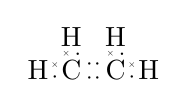
\begin{tikzpicture}[inner sep=0pt]
  \node (c1) at (-0.8em,0){\ce{C}};
  \node (c2) at (0.8em,0){\ce{C}};
  \node (h1) at (-0.8em,1.2em){\ce{H}};
  \node (h2) at (0.8em,1.2em){\ce{H}};
  \node (h3) at (-2.0em,0em){\ce{H}};
  \node (h4) at (2.0em,0em){\ce{H}};
  \draw [draw=none](c1)--(c2)
    node[pos=0.33,below=1pt]{\footnotesize$\cdot$}
    node[pos=0.33,above]{\footnotesize$\cdot$}
    node[pos=0.67,below=1pt]{\footnotesize$\cdot$}
    node[pos=0.67,above]{\footnotesize$\cdot$};
  \foreach \x/\y in {c1/h1,h3/c1,c2/h2,c2/h4}
  {
    \draw [draw=none](\x)--(\y)
      node[midway,sloped,above=0.5pt]{\scalebox{0.35}{$\times$}}
      node[midway,sloped,below=0.5pt]{\footnotesize$\cdot$};
  }
\end{tikzpicture}
\qquad\chemfig{H-C(-[:90]H)=C(-[:90]H)-H}\]

从乙烯的结构式可以看出，乙烯分子里含有 \ce{C=C} 双键，\emph{链烃分子里含有碳碳双键的不饱和烃叫做}\Concept{烯烃}。
乙烯是分子组成最简单的烯烃。

为了更简单形象地描述乙烯分子的结构，我们常用分子模型来表示（\cref{fig:2-7}）。在\cref{fig:2-7a} 的球棍模型里，两个碳原子间用两根可以弯曲的弹性短棍来连接，用它们来表示双键。\cref{fig:2-7b} 是乙烯分子的比例模型。
\begin{figure}
  \begin{minipage}[b]{0.48\linewidth}\centering
    \includegraphics{2-7a.pdf}
    \subcaption{球棍模型}\label{fig:2-7a}
  \end{minipage}
  \begin{minipage}[b]{0.48\linewidth}\centering
    \includegraphics{2-7b.pdf}
    \subcaption{比例模型}\label{fig:2-7b}
  \end{minipage}
  \caption{乙烯分子的模型}\label{fig:2-7}
\end{figure}

实验表明，乙烯分子里的 \ce{C=C} 双键的键长是 \qty{1.33e-10}{m}，乙烯分子里的两个碳原子和四个氢原子都处在同一平面上。
它们彼此之间的键角约为 \ang{120}。
乙烯双键的键能是 \qty{147}{kCal/mol}，实验测得乙烷 \ce{C-C} 单键的键长是 \qty{1.54e-10}{m}，键能是 \qty{83.1}{kCal/mol}。
这表明 \ce{C=C} 双键的键能并不是 \ce{C-C} 单键键能的两倍，而是比两倍略少。
因此，只需要较少的能量，就能使双键里的某一个键断裂。
这从下面介绍的乙烯的化学性质里可以得到证实。

\begin{Reading}[补充阅读]{}
乙烯分子为什么是这样的结构呢？

为了解释 \ce{CH2=CH2} 分子的平面形结构，杂化轨道理论认为碳原子的一个 $2s$ 轨道和两个 $2p$ 轨道进行了 $sp^2$ 杂化（\cref{fig:2-8a}），其余的一个 $p$ 轨道仍保持原状，没有参加杂化。

在构成乙烯分子时，两个碳原子各以 2 个 $sp^2$ 杂化轨道跟两个氢原子的 $1s$ 轨道进行重叠，形成 4 个碳氢的 $\sigma$ 键。
两个碳原子又各以一个 $sp^2$ 杂化轨道相互重叠，形成一个碳碳的 $\sigma$ 键。
分子里所有的 5 个 $\sigma$ 键都在同一平面上，键角约为 \ang{120}（\cref{fig:2-8b}）。
同时，每个碳原子还有一个未参加杂化的 $p$ 轨道，这两个 $p$ 轨道垂直于 5 个 $\sigma$ 键的对称轴所在的平面，并相互平行。
因此，这两个 $p$ 轨道可以在侧面重叠成键（\cref{fig:2-9}）。
这样形成的键叫做 $\pi$ 键。
它垂直于五个 $\sigma$ 键所处的平面。
\begin{figurehere}
  \begin{minipage}{0.3\linewidth}\centering
    \includegraphics{2-8a.pdf}
    \subcaption{}\label{fig:2-8a}
  \end{minipage}
  \begin{minipage}{0.66\linewidth}\centering
    \includegraphics{2-8b.pdf}
    \subcaption{}\label{fig:2-8b}
  \end{minipage}
\end{figurehere}
\begin{figurehere}
  \caption{乙烯分子里的 $\sigma$ 键}\label{fig:2-8}
\end{figurehere}

\begin{figurehere}
  \includegraphics{2-9.pdf}
  \caption{乙烯分子里的 $\pi$ 键}\label{fig:2-9}
\end{figurehere}

由此可见，乙烯分子里的 \ce{C=C} 双键是由一个 $\sigma$ 键和一个 $\pi$ 键形成的。
这两种键的轨道重叠程度是不同的。
$\pi$ 键是由 $p$ 轨道从侧面重叠形成的，重叠程度比 $\sigma$ 键从正面重叠要小，所以 $\pi$ 键不如 $\sigma$ 键牢固，比较容易断裂，断裂时需要的能量也较少。
同时，不象 $\sigma$ 键的电子云那样集中在连接两原子核的对称轴上，而是分散在上下两处。

由于碳原子核对 $\pi$ 键电子云的吸引力比较弱，因此 $\pi$ 键电子云在外界条件的影响下，易于变形。
这就是烯烃为什么较活泼，易于起加成等反应的原因。

已经知道 $\pi$ 键的形成是由于两个互相平行的 $p$ 轨道从侧面重叠的结果，如果这种平行的重叠受到破坏，就会导致 $\pi$ 键的断裂。
所以，双键跟单键不同，以双键相连接的碳原子是不能旋转的。
\end{Reading}

\subsection{乙烯的物理性质}
乙烯是没有颜色的气体，稍有气味，密度是 \qty{1.25}{g/L}，比空气略轻些，难溶于水。

\subsection{乙烯的化学性质和用途}
工业上所用的乙烯，是从石油炼制工厂和石油化工厂所生产的气体里分离出来的。
实验室里是把酒精和浓硫酸混和加热，使酒精分解制得。
浓硫酸在反应过程里起催化剂和脱水剂的作用。
% \[ \ce{ CH3-CH2-OH ->[\text{浓硫酸}][\qty{170}{\celsius}] CH2=CH2 ^ + H2O }\]
\[
\schemestart
\chemname{\chemfig{CH_3-CH_2-OH}}{乙醇}
\arrow(.mid east--.mid west){->[{\footnotesize 浓硫酸}][{\footnotesize \qty{170}{\celsius}}]} 
\chemname{\chemfig{CH_2=CH_2}}{乙烯} \ce{ ^ }
\+ \ce{H2O}
\schemestop\chemnameinit{}
\]
\begin{Experiment}*[righthand ratio=0.6]
把烧瓶和导管等装置如\cref{fig:2-10}。烧瓶里注入酒精和浓硫酸（体积比 $1:3$）的混和液约 \qty{20}{ml}，并放入几片碎瓷，以免混和液在受热沸腾时剧烈跳动。加热使液体温度迅速升到 \qty{170}{\celsius}，这时就有乙烯生成。
\tcblower 
\begin{figurehere}
  \includegraphics{2-10.pdf}
  \caption{乙烯的实验室制法}\label{fig:2-10}
\end{figurehere}
\end{Experiment}

\subsubsection{加成反应}
\begin{Experiment}
把乙烯通入盛溴水的试管里，可以观察到溴水的红棕色很快消失。
\end{Experiment}
乙烯能跟溴水里的溴起反应，生成无色的 1,2-二溴乙烷（\ce{CH2Br-CH2Br}）液体。
\[
\schemestart
\chemfig{H-C(-[:90]H)=C(-[:90]H)-H} \+ \chemfig{Br-Br}
\arrow(.mid east--.mid west)
\chemname{\chemfig{H-C(-[:90]H)(-[:-90]Br)-C(-[:90]H)(-[:-90]Br)-H}}{\footnotesize 1,2-二溴乙烷}
\schemestop\chemnameinit{}
\]

这个反应的实质是乙烯分子里的双键里的一个键易于断裂，两个溴原子分别加在两个价键不饱和的碳原子上，生成了二溴乙烷。
这种\emph{有机物分子里不饱和的碳原子跟其它原子或原子团直接结合生成别的物质的反应叫做}\Concept{加成反应}。

乙烯还能跟氢气、氯气、卤化氢以及水等在适宜的反应条件下起加成反应。
\begin{gather*}
  \ce{CH2=CH2 + H2 ->[\text{催化剂}] CH3-CH3} \\
  \ce{CH2=CH2 + HCl -> CH3-CH2Cl}
\end{gather*}

\subsubsection{氧化反应}
\begin{Experiment}
  点燃纯净的乙烯，它能在空气里燃烧，有明亮的火焰。同时发出黑烟。
\end{Experiment}
跟其它的烃一样，乙烯在空气里燃烧的时候，也生成二氧化碳和水。
但是乙烯分子里含碳量比较大，由于这些碳没有得到充分燃烧，所以有黑烟生成。
下面是乙烯完全燃烧的化学方程式。
\[ \ce{ CH2=CH2 + 3O2 ->[\text{点燃}] 2CO2 + 2H2O \text{（液）} } + \qty{337.2}{kCal} \]

乙烯不但能跟氧气直接发生氧化，并能被氧化剂所氧化。

\begin{Experiment}
  把乙烯通入盛有高锰酸钾溶液（加几滴稀硫酸）的试管里。可以观察到溶液的紫色很快褪去。
\end{Experiment}
乙烯可被氧化剂高锰酸钾（\ce{KMnO4}）氧化，使高锰酸钾溶液褪色。
用这种方法可以区别甲烷和乙烯。

\subsubsection{聚合反应}
在适当的温度、压强和有催化剂存在的条件下，乙烯分子里的双键会断裂其中的一个键，发生加成反应，使乙烯分子里的碳原子能够互相结合成为很长的链。
\begin{multline*} 
  \ce{ CH2=CH2 + CH2=CH2 + CH2=CH2 } \cdots\cdots \ce{ -> }\\
  \ce{-CH2-CH2- + -CH2-CH2- + -CH2-CH2- } \cdots\cdots \\
  \ce{ -> -CH2-CH2-CH2-CH2-CH2-CH2- } \cdots\cdots
\end{multline*}

这个反应还可以用下式表示：
\[ 
\schemestart
$n$\,\chemfig{CH_2=CH_2}
\arrow(.mid east--.mid west){->[\scriptsize 催化剂]}
\chemname{\chemfig{\vphantom{CH_2}-[@{op,.6}]CH_2-CH_2-[@{cl,0.4}]}\polymerdelim[delimiters ={[]},indice =\!n]{op}{cl}}{\footnotesize 聚乙烯}
\schemestop\chemnameinit{}
\]

反应的产物是聚乙烯。
它是一种式量很大（几万到几十万）的化合物，它的化学式可以简单地写为 \ce{(C2H4)_$n$}。
生成聚乙烯这样的反应属于聚合反应。
在这个聚合反应里，式量小的化合物分子互相结合为式量很大的化合物分子。
这样的聚合反应也是加成反应，所以又属于\Concept{加成聚合反应}，简称\Concept{加聚反应}。

从六十年代以来，世界上乙烯的产量飞速发展。
乙烯是石油化学工业最重要的基础原料，用于制造塑料、合成纤维、有机溶剂等。
乙烯的发展带动了其它石油化工基础原料和产品的发展。

乙烯还是一种植物生长调节剂，例如它可被用做果实催熟剂等。

\begin{Practice}[习题]
\begin{question}
  \item 怎样鉴别装在不同容器里的甲烷和乙烯？
  \item 在实验室里怎样从混有乙烯的甲烷里提纯甲烷？
  \item 当乙烯通过装有溴的试剂瓶的时候，试剂瓶的质量增加了 \qty{16}{g}。有多少升的乙烯（在标准状况下）被吸收了？生成了多少克的二溴乙烷？
  \item 乙烯跟氯化氢加成可以生成氯乙烷（\ce{C2H5Cl}），写出反应的化学方程式。按理论计算每吨乙烯能生产多少吨氯乙烷？
\end{question}
\end{Practice}

\section{烯烃}
\subsection{烯烃及其命名}
烯烃是分子里含有碳碳双键（\ce{C=C}）的不饱和链烃的总称。
烯烃里除乙烯外，还有丙烯（\ce{CH3CH=CH2}），丁烯（\ce{CH3CH2CH=CH2}）等等。\cref{tab:2-2} 列举几种乙烯的同系物的物理性质。
\begin{table}
  \caption{几种烯烃的物理性质}\label{tab:2-2}
  \begin{tblr}{colspec={cX[r]cS[table-format=5.2]S[table-format=5.2]l},hline{2}=0.8pt,row{1}={m,c,guard}}
    名称 & 结构简式 & {常温时\\状态} & 熔点 \unit{\celsius} & 沸点 \unit{\celsius} & {液态时的密度\\（\unit{g/cm^3}）}\\
    乙烯 & \ce{CH2=CH2}         & 气 & -169.2 & -103.7 & $0.384^*$ \\
    丙烯 & \ce{CH3CH=CH2}       & 气 & -185.3 & -47.4  & $0.5193$ \\
    丁烯 & \ce{CH3CH2CH=CH2}    & 气 & -185.4 & -6.3   & $0.5951$ \\
    戊烯 & \ce{CH3(CH2)2CH=CH2} & 液 & -138   & 29.97  & $0.6405$ \\
    己烯 & \ce{CH3(CH2)3CH=CH2} & 液 & -139.8 & 63.35  & $0.6731$ \\
    庚烯 & \ce{CH3(CH2)4CH=CH2} & 液 & -119   & 93.64  & $0.6970$ \\
  \end{tblr}\par
  \begin{minipage}{\linewidth}
    \footnotesize * 是 \qty{-10}{\celsius} 时的值，其余是 \qty{20}{\celsius} 时的值。
  \end{minipage}
\end{table}

由\cref{tab:2-2} 我们可以看出，跟烷烃一样，乙烯同系物也是依次相差一个 \ce{CH2} 原子团。
烯烃的通式是 \ce{C_$n$H_$2n$}。
它们的物理性质一般地也随着碳原子数目的增加而递变。
烯烃的化学性质也跟乙烯类似，如易于起加成反应等。

丙烯是石油工业的一种重要产品，也是一种重要的化工原料。
例如，通过加聚反应制造聚丙烯。

烯烃的命名跟烷烃类似，所不同的是要求表示出双键的位置。
命名的步骤是：
\begin{enumerate}[1.]
  \item 确定包括双键在内的碳原子数目最多的碳链为主链。
  \item 主链里碳原子的依次编号从离双键较近的一端算起。
  \item 双键的位置可以用阿拉伯数字标在某烯字样的前面。

  例如：
  \[ 
\schemestart
\chemname{\chemfig{CH_2=CHCH_2CH_3}}{\footnotesize 1-丁烯}\quad
\chemname{\chemfig{CH_3CH=CHCH_3}}{\footnotesize 2-丁烯}\quad
\chemname{\chemfig{CH_3-CH=CH-CH(-[:-90]CH_3)-CH_3}}{\footnotesize 4-甲基-2-丁烯}
\schemestop\chemnameinit{}
\]
  1-丁烯和 2-丁烯是同分异构体。
\end{enumerate}

\subsection{二烯烃}
分子里含有两个双键的链烃叫做二烯烃，如 1,3-丁二烯（\chemfig{\charge{90[anchor=-90]={\tiny 1}}{C}H_2=\charge{90[anchor=-90]={\tiny 2}}{C}H\charge{90[anchor=-90]={\tiny 3}}{C}H=\charge{90[anchor=-90]={\tiny 4}}{C}H_2}）就是二烯烃里的最重要的同系物。
1,3-丁二烯是一种重要的有机化工原料。

二烯烃有双键，也象烯烃一样能起加成反应等。
但是，1,3-丁二烯有两个双键，又有它的特点，在起加成反应时，两个双键里比较活泼的键能够一起断裂，而同时又生成一个新的双键。
例如，1,3-丁二烯跟 \ce{Br2} 进行的加成反应。
\[ \schemestart
\chemfig{\charge{90[anchor=-90]={\tiny 1}}{C}H_2=\charge{90[anchor=-90]={\tiny 2}}{C}H-\charge{90[anchor=-90]={\tiny 3}}{C}H=\charge{90[anchor=-90]={\tiny 4}}{C}H_2} \+ \ce{Br2} \arrow \chemfig{Br-\charge{90[anchor=-90]={\tiny 1}}{C}H_2-\charge{90[anchor=-90]={\tiny 2}}{C}H=\charge{90[anchor=-90]={\tiny 3}}{C}H-\charge{90[anchor=-90]={\tiny 4}}{C}H_2-Br}
\schemestop\chemnameinit{}\]
这种形式的加成反应叫 1,4-加成反应。

除生成这种 1,4 加成的产物外，还生成 1,2-加成产物：
\[ \chemfig{Br-\charge{90[anchor=-90]={\tiny 1}}{C}H_2-\charge{90[anchor=-90]={\tiny 2}}{C}HBr-\charge{90[anchor=-90]={\tiny 3}}{C}H=\charge{90[anchor=-90]={\tiny 4}}{C}H_2 } \]

在 1,3-丁二烯的加成反应里，1,4-加成产物通常是主要的。
1,4-加成反应在生产中有重要的意义。

二烯烃比烯烃多一个双键，少两个氢原子，所以二烯烃的通式是 \ce{C_$n$H_$2n-2$}。

\begin{Practice}
\begin{question}
  \item 写出式量是 56 的某链烃的各种同分异构体的结构式，并写出它们的名称。
  \item 写出\begin{enumerate*}\item 丙烯、\item 异丁烯\end{enumerate*}的电子式。
  \item 写出下列各烯烃的同分异构体的数目，并写出它们的结构式：
  \[\chemfig{CH_2=C(-[:-90]CH_3)-CH_3} \quad \chemfig{CH_3-CH=CH-CH_2-CH_3} \]
  \item 写出下列几种物质的结构简式：
  \begin{tasks}(3)
    \task  丙烯，
    \task  1-丁烯，
    \task  1,3-丁二烯，
    \task! 异戊二烯（即 2-甲基-1,3-丁二烯）。
  \end{tasks}
  \item 某种烃的化学式是 \ce{C5H10}，我们能不能说它一定是乙烯的同系物？为什么？
  \item 从环烷烃的化学式来看，它是哪一类链烃的同分异构体？
  \item 某烃 \qty{0.1}{mol} 完全燃烧后，生成 \qty{0.3}{mol} \ce{CO2} 和 \qty{0.3}{mol} \ce{H2O}，这种烃的化学式是什么？
\end{question}
\end{Practice}

\section[乙炔\ 炔烃]{乙炔\texorpdfstring{\protect\footnote{炔音\pinyin{que1}}\quad}{ }炔烃}
\subsection{乙炔的物理性质和结构式}
乙炔俗名电石气，纯的乙炔是没有颜色、没有臭味的气体，由电石制备的乙炔常因混有磷化氢、硫化氢等杂质而发出特殊难闻的臭味。
乙炔的密度是 \qty{1.16}{g/L}，比空气稍轻，微溶于水，易溶于有机溶剂。

乙炔的化学式是 \ce{C2H2}。从这个化学式可以看出，乙炔的分子比乙烯的分子少两个氢原子。
在乙炔分子里的碳原子间有三个共用电子对。
通常我们把它称为叁键，这可用下式表示：
\[ \quad \chemfig{H-C~C-H}\]

\cref{fig:2-11} 是乙炔分子的两种模型。
\begin{figure}
  \begin{minipage}[b]{0.48\linewidth}\centering
    \includegraphics{2-11a.pdf}
    \subcaption{球棍模型}\label{fig:2-11a}
  \end{minipage}
  \begin{minipage}[b]{0.48\linewidth}\centering
    \includegraphics{2-11b.pdf}
    \subcaption{比例模型}\label{fig:2-11b}
  \end{minipage}
  \caption{乙炔的分子模型}\label{fig:2-11}
\end{figure}

实验表明，乙炔分子里碳碳之间的叁键的键能是 \qty{194}{kCal/mol}，并不等于三个单键键能之和，比三个单键的键能要小得多（也比一个单键和一个双键键能之和小）。
叁键的键长是 \qty{1.20e-10}{m}，比单键和双键的键长都短。
并且已经证明乙炔分子里 \ce{C#C} 键跟 \ce{C-C} 键间的夹角是 \ang{180}，也就是说，乙炔分子里的两个碳原子和两个氢原子处在一条直线上。

\begin{Reading}[补充阅读]{}
乙炔分子为什么有这样的结构呢？
\begin{figurehere}
  \begin{minipage}[b]{0.4\linewidth}\centering
    \includegraphics{2-12a.pdf}
    \subcaption{$sp$ 杂化}\label{fig:2-12a}
  \end{minipage}
  \begin{minipage}[b]{0.58\linewidth}\centering
    \includegraphics{2-12b.pdf}
    \subcaption{$\sigma$ 键的形成}\label{fig:2-12b}
  \end{minipage}
  \caption{乙炔分子里 $\sigma$ 模型}\label{fig:2-12}
\end{figurehere}

杂化轨道理论对于乙炔分子结构的解释是，乙炔分子里每个碳原子在形成叁键时，是以一个 $2s$ 轨道和一个 $2p$ 轨道进行杂化，形成两个能量相等的沂轨道，叫做 $sp$ 杂化轨道（\cref{fig:2-12a}）。
这两个 $sp$ 杂化轨道的对称轴在同一条直线上。
每个碳原子各以一个 $sp$ 杂化轨道跟氢原子的一个 $1s$ 轨道进行重叠而形成一个碳氢的 $\sigma$ 键。
同时又各以其另一个 $sp$ 杂化轨道相互重叠形成一个碳碳的 $\sigma$ 键（\cref{fig:2-12b}）。
在两个碳原子里还各有另外两个 $p$ 轨道没有参加杂化，它们的电子云互相垂直，同时也跟碳碳间 $\sigma$ 键的对称轴垂直。
这样就在 4 个 $p$ 电子之间形成两个 $\pi$ 键,这两个 $\pi$ 键是互相垂直的（\cref{fig:2-13}）。

\begin{figurehere}
  \includegraphics{2-13.pdf}
  \caption{乙炔分子里 $\pi$ 键的形成}\label{fig:2-13}
\end{figurehere}

乙炔分子里的 \ce{C#C} 叁键是由一个 $\sigma$ 键和两个相互垂直的 $\pi$ 键所组成。
已知 $\pi$ 键键能小于 $\sigma$ 键键能，所以在一定条件下，$\pi$ 键容易断裂。
因此，具有叁键的化合物也很活泼，如易起氧化反应、加成反应等。
同时，叁键的键长也比双键更短一些。
\end{Reading}

\subsection{乙炔的制法、化学性质和用途}
\subsubsection{实验室制法}
乙炔在实验室里是用电石（碳化钙）跟水反应制得。
\[ \ce{ CaC2 + 2H2O -> C2H2 + Ca(OH)2} + \qty{30.33}{KCal} \]

\begin{Experiment}*[righthand ratio=0.5]\label{expr:2-9}
  实验装置如\cref{fig:2-14} 所示。在广口瓶里放几小块碳化钙。轻轻旋开分液漏斗的活栓，使水\footnote{碳化钙跟水的反应比较剧烈，为了得到平稳的乙炔气流，可以用包和食盐水代替水。食盐跟碳化钙不起反应。}缓慢地滴下。用排水法收集乙炔。观察乙炔的颜色、状态。
  \tcblower
  \begin{figurehere}
    \includegraphics{2-14.pdf}
    \caption{制取乙炔}\label{fig:2-14}
  \end{figurehere}
\end{Experiment}

\subsubsection{乙炔的化学性质}
\paragraph{氧化反应}\mbox{}\par
\begin{Experiment}
  点燃从\cref{expr:2-9} 制取的乙炔，观察火焰。
\end{Experiment}
乙炔完全燃烧的反应可以表示如下：
\[ \ce{ 2C2H2 + 5O2 ->[\text{点燃}] 4CO2 + 2H2O\,\text{（液）}} + \qty{621.2}{kCal}\]

乙炔燃烧时产生大量的热。
乙炔的成分里含碳量很大，所以燃烧不充分时发出光亮而带浓烟的火焰。乙炔跟空气的混和物遇火会发生爆炸\footnote{乙炔在空气里的爆炸极限是含乙炔 2.5\%～80\%。}，所以在生产和使用乙炔时,必须注意安全。
乙炔在氧气里燃烧时，产生的氧炔焰的温度很高（可达 \qty{3000}{\celsius} 以上），可以用来切割和焊接金属。
\begin{Experiment}
把纯净的乙炔通入盛有高锰酸钾溶液（加少量硫酸）的试管，观察紫色溶液的变化。
\end{Experiment}
乙炔也容易被氧化剂所氧化，能使高锰酸钾溶液的紫色褪去。

\paragraph{加成反应}\mbox{}\par
\begin{Experiment}
  把纯净的乙炔通入盛有溴水的试管，观察溶液颜色的变化。
\end{Experiment}
可以观察到乙炔也能使溴水褪色。反应过程可以分步表示如下：
\begin{gather*}
\schemestart
\chemfig{H-C~C-H} \+ \chemfig{Br-Br} \arrow(.mid east--.mid west)
\chemname{\chemfig{H-C(-[:-90]Br)=C(-[:-90]Br)-H}}{\footnotesize 1,2-二溴乙烯}
\schemestop\chemnameinit{}\\
\schemestart
\chemfig{H-C(-[:-90]Br)=C(-[:-90]Br)-H} \+ \chemfig{Br-Br} \arrow(.mid east--.mid west)
\chemname{\chemfig{H-C(-[:-90]Br)(-[:90]Br)-C(-[:-90]Br)(-[:90]Br)-H}}{\footnotesize 1,1,2,2-四溴乙烷}
\schemestop\chemnameinit{}
\end{gather*}

如果用镍粉作催化剂并且加热，乙炔就能跟氢气进行加成反应，先生成乙烯，再成为乙烷。
\begin{gather*}
  \ce{   CH#CH + H2 ->[\text{催化剂}][\triangle] CH2=CH2} \\
  \ce{ CH2=CH2 + H2 ->[\text{催化剂}][\triangle] CH3-CH3} 
\end{gather*}

乙炔跟溴、氢气的加成反应，有力地证明了乙炔结构式的正确性。

在 \qtyrange{150}{160}{\celsius} 和氯化汞作为催化剂的条件下，乙炔能跟氯化氢进行加成反应，生成氯乙烯。
氯乙烯是重要的化工原料。
% \[ \ce{ HC#CH + HCl ->[\text{催化剂}][\triangle] CH2=CHCl } \]
\[\schemestart
\chemfig{HC~CH} \+ \chemfig{HCl} 
\arrow(.mid east--.mid west){->[\footnotesize 催化剂][\footnotesize $\triangle$]}
\chemname{\chemfig{CH_2=CHCl}}{\footnotesize 氯乙烯}
\schemestop\chemnameinit{}\]

\subsubsection{乙炔的用途}
从乙炔的性质可以知道，由乙炔开始能制出氯乙烯等许多重要有机化学工业的原料，所以乙炔是一种重要的基本有机原料。
但是，从电石生产乙炔，需要消耗大量的电，所以今后趋向于用天然气和石油作为原料来生产乙炔。

\subsection{炔烃}
\emph{链烃分子里含有碳碳叁键的不饱和烃叫做}\Concept{炔烃}。
除乙炔外还有丙炔、丁炔等等。
\cref{tab:2-3} 是几种乙炔同系物的名称、结构简式和物理性质。
\begin{table}
  \caption{几种块烃的物理性质}\label{tab:2-3}
  \begin{tblr}{colspec={cX[r]cS[table-format=5.2]S[table-format=5.2]l},hline{2}=0.8pt,row{1}={m,c,guard}}
    名称 & 结构简式 & {常温时\\状态} & 熔点 \unit{\celsius} & 沸点 \unit{\celsius} & {液态时的密度\\（\unit{g/cm^3}）}\\
    乙炔   & \ce{H-C#CH}           & 气 & -80.8 & -84.0 & $0.6181^*$ \\
    丙炔   & \ce{CH3-C#CH}        & 气 & -101.5 & -23.2 & $0.66^{**}$ \\
    1-丁炔 & \ce{CH3-CH2-C#CH}    & 气 & -125.7 & 8.1 & $0.6784^{***}$ \\
    1-戊炔 & \ce{CH3-(CH2)2-C#CH} & 液 & -90 & 40.18 & $0.6901$ \\
  \end{tblr}\par
  \begin{minipage}{\linewidth}
    \footnotesize * 是 \qty{-32}{\celsius} 时的值，** 是 \qty{-13}{\celsius} 时的值，*** 是 \qty{0}{\celsius} 时的值，另一是 \qty{20}{\celsius} 时的值。
  \end{minipage}
\end{table}

从\cref{tab:2-3} 可知，乙炔的各同系物也依次相差一个 \ce{CH2} 原子团，但它们比同级的烯烃各少两个氢原子，所以炔烃的通式是 \ce{C_$n$H_$2n-2$}。
炔烃的物理性质一般也是随着分子里碳原子数的增多而递变的。

\begin{Practice}[习题]
\begin{question}
  \item 使 \qty{13}{g} 乙炔完全燃烧，在 \qty{1}{atm} 和 \qty{27}{\celsius} 时需要用多少升空气？
  \item 比较乙烷、乙烯、乙炔的化学性质。
  \item 相同摩尔数的乙烷、乙烯和乙炔完全燃烧后生成的二氧化碳和水的量是不是相等？产生的热量是不是相等？用热化学方程式来说明。
  \item 指出下列化学式各代表哪类直链烃：
  \begin{tasks}(5)
    \task \ce{C8H16}，
    \task \ce{C9H16}，
    \task \ce{C15H32}，
    \task \ce{C17H34}，
    \task \ce{C7H12}。
  \end{tasks}
  \item 哪类烃叫做不饱和链烃？你所知道的不饱和链烃可以分成哪几类？不饱和链烃具有哪些特性？
  \item 在标准状况下，\qty{11.2}{L} 乙炔跟溴起加成反应，需要溴的最大数量是多少克？
  \item 含杂质 10\% 的碳化钙 \qty{100}{g}，在 \qty{25}{\celsius} 和 \qty{770}{mmHg} 时能够制得乙炔多少升？
  \item 通式为 \ce{C_$n$H_$2n-2$} 的一种炔烃完全燃烧后，生成的 \ce{CO2} 和 \ce{H2O} 的摩尔数比是 $2:1$，写出这种炔烃的化学式。
\end{question}
\end{Practice}

\section[苯\  芳香烃]{苯\texorpdfstring{\protect\footnote{苯音\pinyin{ben3}}\quad}{ }芳香烃}
\subsection{苯分子的结构}
苯是没有颜色带有特殊气味的液体，比水轻，不溶于水。
苯的沸点是 \qty{80.1}{\celsius}，熔点是 \qty{5.5}{\celsius}。
如果用冰来冷却，苯可以凝结成无色的晶体。

苯的化学式是 \ce{C6H6}。
从苯的化学式看，苯是远没有达到饱和的烃。
因为苯的分子需要增加 8 个氢原子才符合饱和链烃的通式： \ce{C_$n$H_$2n+2$}。
根据长期研究，认为苯的结构式可以这样表示：
\[
\chemfig{C*6(=C(-[:-90]H)-C(-[:0]H)=C(-[:0]H)-C(-[:90]H)=C(-[:180]H)-)(-[:180]H)}
\quad \text{或者简写为}\ \chemfig{*6(=-=-=-)} \]

从这样的结构式（又称凯库勒式）来推测，苯的化学性质应该显示出不饱和烃的性质。
是不是这样呢？让我们仔细观察下面的实验。
\begin{Experiment}
在盛有苯的两个试管里，分别加入高锰酸钾的酸性溶液和溴水，结果溶液颜色都保持不变。这说明苯跟高锰酸钾溶液或溴水都不起反应。
\end{Experiment}

由此可知，苯跟一般烯烃在性质上有很大区别。

对苯的结构作进一步的研究后知道，苯分子具有平面的正六边形结构。
各个键角都是 \ang{120}，六角环上碳碳之间的键长都是 \qty{1.40e-10}{m}。
它既不同于一般的单键（\ce{C-C} 键键长是 \qty{1.54e-10}{m}），也不同于一般的双键（\ce{C=C} 键键长是 \qty{1.33e-10}{m}）。

从苯跟高锰酸钾溶液和溴水都不起反应这一事实和测定的碳碳间键长的实验数据来看，充分说明苯环上碳碳间的键应是一种介于单键和双键之间的独特的键。
为了表示苯分子结构这一特点，常用右式来表示苯的结构简式 \chemfig[atom sep=0.5em]{[:30]**6(------)}。

苯分子模型可以如\cref{fig:2-15} 那样表示：
\begin{figure}
  \includegraphics{2-15.pdf}
  \caption{苯分子模型}\label{fig:2-15}
\end{figure}

直到现在，凯库勒式的表示方法仍被沿用，但在使用时绝不应认为苯是单、双键交替组成的环状结构。

在有机化合物里有一大类化合物叫做芳香族化合物\footnote{在已知的芳香族化合物里，大都是没有香味的。现在芳香族化合物这个名称已失去了它原来的意义（历史上是指一类从植物胶里取得的具有芳香气味的物质），只是因为使用这个名词已经习惯了，所以沿用到现在。}。\emph{分子里含有一个或多个苯环的化合物属于芳香族化合物}。
因此，我们可以说，苯环是芳香族化合物的母体。
苯是最简单、最基本的芳烃。

\begin{Reading}[补充阅读]{}
苯分子为什么是这样的结构呢？

按照杂化轨道理论，苯分子里六个碳原子的电子都以 $sp^2$ 杂化轨道相互重叠，形成六个碳碳的 $\sigma$ 键，又各以一个 $sp^2$ 杂化轨道分别跟氢原子的 \({1s}\) 轨道进行重叠，形成 6 个碳氢的 $\sigma$ 键。
由于是 $sp^2$ 杂化，所以键角是 \ang{120}，并且所有 6 个碳原子和 6 个氢原子都是在同一平面上相互连接起来的（\cref{fig:2-16}）。苯环上六个碳原子各有一个未参加杂化的 $2p$ 轨道，它们垂直于环的平面，并从侧面相互重叠而形成一个闭合的 $\pi$ 键（\cref{fig:2-17}），
\begin{figurehere}
  \nextfloat
  \begin{minipage}[b]{0.48\linewidth}\centering
    \includegraphics{2-16a.pdf}
    \subcaption{轨道重叠成 $\sigma$ 键}\label{fig:2-16a}
  \end{minipage}
  \begin{minipage}[b]{0.48\linewidth}\centering
    \includegraphics{2-16b.pdf}
    \subcaption{$\sigma$ 键分布示意图}\label{fig:2-16b}
  \end{minipage}
  \caption{苯分子内 $\sigma$ 键形成示意图}\label{fig:2-16}
\end{figurehere}
并且均匀地对称分布在环平面的上方和下方。
通常把苯的这种键型称为大 $\pi$ 键。
苯的大 $\pi$ 键的形成使 $\pi$ 键电子云不是只为某两个碳原子所共用，而是为 6 个碳原子所共用，因而受到六个碳原子核的共同吸引，彼此结合得比较牢固。
所以苯的性质比不饱和烃稳定，如在通常情况下不易发生一般不饱和烃所容易发生的加成反应等。
同时，苯的大 $\pi$ 键是平均分布在六个碳原子上，所以苯分子中每个碳碳键的键长和键能是相等的。
\begin{figurehere}
  \nextfloat
  \begin{minipage}[b]{0.48\linewidth}\centering
    \includegraphics{2-17a.pdf}
    \subcaption{$p$ 轨道重叠}\label{fig:2-17a}
  \end{minipage}
  \begin{minipage}[b]{0.48\linewidth}\centering
    \includegraphics{2-17b.pdf}
    \subcaption{大 $\pi$ 键的形成}\label{fig:2-17b}
  \end{minipage}
  \caption{苯分子大 $\pi$ 键的形成}\label{fig:2-17}
\end{figurehere}
\end{Reading}

\subsection{苯的化学性质和用途}
\subsubsection{取代反应}
苯分子里的氢原子能分别被别的原子或原子团所取代。

\paragraph{苯跟卤素的取代反应}\mbox{}\par
\begin{Experiment}*[righthand ratio=0.4]
把苯和少量液态溴放在烧瓶里，同时加入少量铁屑作催化剂\footnote{实际上起催化作用的是铁跟溴反应生成的溴化铁（\ce{FeBr3}）。}。用带导管的瓶塞塞紧瓶口（\cref{fig:2-18}），跟瓶口垂直的一段导管可以兼起冷凝器的作用。在常温时，很快就会看到，在导管口附近出现白雾（由溴化氢遇水蒸气所形成）。反应完毕后,向锥形瓶里的液体里滴入 \ce{AgNO3} 溶液，有浅黄色溴化银沉淀生成。把烧瓶里的液体倒在盛有冷水的烧杯里，烧杯底部有褐色不溶于水的液体。
\tcblower
\begin{figurehere}
  \includegraphics{2-18.pdf}
  \caption{苯跟溴的取代反应}\label{fig:2-18}
\end{figurehere}
\end{Experiment}
不溶于水的液体是溴苯，它是比水重的无色液体，由于溶解了溴而显褐色。苯跟溴的取代反应可以用化学方程式表示如下：
\[
\schemestart
\chemfig{[:-30]*6(=-=-=-)} \+ \chemfig{Br_2}
\arrow(.mid east--.mid west){->[\footnotesize 催化剂]}
\chemname{\chemfig{[:-30]*6(=-=(-Br)-=-)}}{\footnotesize 溴苯}
\+ \chemfig{HBr}
\schemestop\chemnameinit{}
\]

在催化剂作用下，苯也能跟其它卤素起取代反应。

\paragraph{苯的硝化反应}\mbox{}\par
\begin{Experiment}
在一个大试管里，先加入 \qty{1.5}{ml} 浓硝酸和 \qty{2}{ml} 浓硫酸，摇匀，冷却到 \qtyrange{50}{60}{\celsius} 以下，然后慢慢地滴入 \qty{1}{ml} 苯，不断摇动，使混和均匀，然后放在 \qty{60}{ \celsius} 的水浴中加热 \qty{10}{min}，把混和物倒入另一个盛水的试管里。可以明显地看到，有一种油状物生成。
\end{Experiment}

这种油状液体是硝基苯 \ce{C6H5NO2}，反应的化学方程式可以表示如下：
\[
\schemestart
\chemfig{[:-30]*6(=-=-=-)} \+ \chemfig{HO-NO_2}
\arrow(.mid east--.mid west){->[\footnotesize 催化剂][\footnotesize $\triangle$]}
\chemname{\chemfig{[:-30]*6(=-=(-NO_2)-=-)}}{\footnotesize 硝基苯}
\+ \chemfig{H_2O}
\schemestop\chemnameinit{}
\]

苯分子里的氢原子被 \ce{-NO2} 所取代的反应，叫做\Concept{硝化反应}。
硝酸分子里的 \ce{-NO2} 原子团叫做\Concept{硝基}。

硝基苯是一种没有颜色的油状液体，不纯的显淡黄色。
硝基苯有苦杏仁气味，比水重，有毒，是制造染料的重要原料。

\paragraph{苯的磺化反应}\mbox{}\par
共热到 \qtyrange{70}{80}{\celsius}，苯跟浓硫酸起反应。
在这个反应里，苯分子里的氢原子被硫酸分子里的\Concept{磺酸基}（\ce{-SO3H}）所取代而生成苯磺酸（\ce{C6H5-SO3H}）。这种反应叫做\Concept{磺化反应}。
\[
\schemestart
\chemfig{[:-30]*6(=-=-=-)} \+ \chemfig{HO-SO_3H}
\arrow(.mid east--.mid west){->[\footnotesize $\triangle$]}
\chemname{\chemfig{[:-30]*6(=-=(-SO_3H)-=-)}}{\footnotesize 苯磺酸}
\+ \chemfig{H_2O}
\schemestop\chemnameinit{} 
\]

苯的硝化反应和磺化反应都属于取代反应。

\subsubsection{加成反应}
苯不具有典型的双键所应有的加成反应性能，但在特殊情况下，它仍能够起加成反应。
如有镍催化剂存在和在 \qtyrange{180}{250}{\celsius} 的条件下，苯可以跟氢起加成反应，即生成饱和环烃。
\[
\schemestart
\chemfig{*6(-=-=-=)} \+ \chemfig{3H_2}
\arrow(.mid east--.mid west){->[\footnotesize 催化剂][\footnotesize $\triangle$]}
\chemname{\chemfig{H_2C*6(-C(-[:-90,0.5,,,line width=0pt]H_2)-CH_2-CH_2-C(-[:90,0.5,,,line width=0pt]H_2)-C(-[:180,0.5,,,line width=0pt]H_2)-)}}{\footnotesize 环己烷}
\schemestop\chemnameinit{}
\]

在光照条件下，苯跟氯气起加成反应，生成六氯环己烷（\ce{C6H6Cl6}），它曾是一种使用较广的农药，即六六六，有杀虫作用。
但由于它的化学性质稳定，能在动植物体内和环境中累积，容易污染环境和食物。
因此，对六六六采取了限制使用和用高效、低毒、低残留的新品种农药取代的措施。

\subsubsection{苯在空气里燃烧}
苯在空气里能燃烧生成二氧化碳和水，燃烧时发生明亮并带有浓烟的火焰，这由于苯分子里含碳量很大的缘故。

苯是一种很重要的有机化工原料，它广泛用来生产合成纤维、合成橡胶、塑料、农药、医药、染料、香料等。
苯也常用作有机溶剂。

在从前，苯是从炼焦所得的煤焦油里提取的，产量受到一定的限制。
自从石油工业迅速发展以来，大量的苯可以从石油工业获得。

\medskip
\begin{Theorem}{讨论}
比较苯跟甲烷、乙烯的化学性质，你对苯跟烷烃和烯烃的性质既相似又不相似的事实怎样理解？
\end{Theorem}

\subsection{苯的同系物}
甲苯 \ce{C7H8}、二甲苯 \ce{C8H10} 等化合物的分子里都含有一个苯环结构。
它们都是苯的同系物。
苯的同系物的通式是 \ce{C_$n$H_$2n-6$}（$n\geqslant6$）。
它们都是芳香烃。
苯分子里的一个氢原子被甲基 \chemfig{CH_3-} 取代后生成甲苯 \chemfig[atom sep=0.7em]{[:30]*6(=-(-[:0,2]CH_3)=-=-)}。
两个氢原子被两个甲基取代后生成二甲苯。
由于取代位置不同，二甲苯有下列三种异构体：
\[\schemestart 
\chemname{\chemfig{[:-30]*6(-=-=(-[:90]CH_3)-(-[:90]CH_3)=)}}{\footnotesize 邻-二甲苯\\（沸点：\qty{144.4}{\celsius}）}\qquad\qquad
\chemname{\chemfig{CH_3-*6(-=-=(-[:90]CH_3)-=)}}{\footnotesize 间-二甲苯\\（沸点：\qty{139.1}{\celsius}）}\qquad
\chemname{\chemfig{CH_3-*6(-=-(-CH_3)=-=)}}{\footnotesize 对-二甲苯\\（沸点：\qty{138.4}{\celsius}）}
\schemestop\chemnameinit{}\]

苯的同系物在性质上跟苯有许多和似之处，如燃烧时都发生带有浓烟的火焰，也都能起取代反应等。

由于苯环和侧链的相互影响，使苯的同系物也有一些化学性质跟苯不同。
\begin{Experiment}
把甲苯、二甲苯各 \qty{2}{ml} 分别注入两个试管，各加入高锰酸钾酸性溶液 3 滴，用力振荡，结果紫色褪去。
\end{Experiment}
这一实验说明，甲苯、二甲苯能被高锰酸钾氧化，但被氧化的是苯环上的侧链，即甲基。

我们已经学过链烃、环烃和芳烃，为了区别于成环的环烷烃、芳烃等，链烃又叫脂肪烃。
脂肪烃因跟脂肪类物质有类似结构而得名。

\subsection[萘和蒽]{萘和蒽\texorpdfstring{\protect\footnote{萘音\pinyin{nai4},蒽音\pinyin{en1}}}{}}
在煤焦油里除了可以提取苯及其同系物外，还可以提取萘和蒽等其它芳香烃。
\subsubsection{萘（\ce{C10H8}）}
萘是一种重要的化工原料，它的结构式是：
\[ \chemfig{C*6(=C(-[:-90]H)-C(*6(-C(-[:-90]H)=C(-[:0]H)-C(-[:0]H)=C(-[:90]H)-#(,6pt)))=C-C(-[:90]H)=C(-[:180]H)-)(-[:180]H)} \quad \text{或简写成}\quad \chemfig{*6(=-(*6(-=-=-))=-=-)}\]

萘是一种无色片状的晶体，熔点为 \qty{80.55}{\celsius}，具有特殊的气味。
它不溶于水，易升华。
萘可以用来杀菌、防蛀、驱虫。
日常用的卫生球的主要成分就是萘。

\subsubsection{蒽（\ce{C14H10}）}
蒽也是一种重要的化工原料，它的结构式是：
\[ \chemfig{C*6(=C(-[:-90]H)-C(*6(C-C(-[:-90]H)=C(*6(-C(-[:-90]H)=C(-[:0]H)-C(-[:0]H)=C(-[:90]H)-#(,6pt)))-C=C(-[:90]H)-#(,6pt)))=C-C(-[:90]H)=C(-[:180]H)-)(-[:180]H)} \ \text{或简写成}\ \chemfig{*6(=-(*6(-=(*6(-=-=-))-=-))=-=-)} \]

蒽也是一种无色的晶体，熔点为 \qty{216.2}{\celsius}，易升华。
蒽是生产染料的重要原料。

萘和蒽都是由两个或两个以上的苯环分别共用相邻的碳原子而成的芳香烃。
这种芳香烃特称为稠环芳香烃。

\begin{Practice}[习题]
\begin{question}
  \item 怎样通过实验来区别苯、己烷和己烯？
  \item 某烃的化学式是 \ce{C8H10}，它不能使溴水褪色，但能使高锰酸钾酸性溶液褪色，能跟氢起加成反应，生成乙基环己烷。写出这种烃的结构式。
  \item 下列各种化合物各属于哪一类烃？写出它们的名称和结构式：
  \begin{tasks}(4)
    \task \ce{C6H5-C3H7}，
    \task \ce{C6H14}，
    \task \ce{C6H6}，
    \task \ce{C3H6}，
    \task \ce{C2H2}，
    \task*(2) \ce{CH3-CH2-CH=CH2}，
    \task \ce{C3H4}，
    \task \ce{C10H8}。
  \end{tasks}
\end{question}
\end{Practice}

\section{石油和石油产品概述}
烃的自然界来源主要是石油和天然气。
天然气的主要成分是甲烷，它含甲烷可达 80\%～98\%（体积百分比）。
有的天然气还含有乙烷、丙烷，以及 \ce{CO2}、\ce{N2} 等等，常因产地的不同，成分也有差别。
天然气是一种优良的气体燃料。

石油是一种极其重要的资源，是发展国民经济和国防建设的重要物资。
通过石油炼制，可以得到汽油、煤油、柴油等燃料和各种机器所需要的润滑油以及许多气态烃（称为炼厂气）等产品。
用石油产品和石油气（炼厂气、油田气、天然气）做原料来生产化工产品的工业简称石油化工。
利用石油产品做原料，通过化工过程，可以制造合成纤维、合成橡胶、塑料以及农药、化肥、炸药、医药、染料、油漆、合成洗涤剂等产品。
石油产品已被广泛地应用到国民经济各个部门。
所以人们把石油称为“工业的血液”。

\subsection{石油的成分}
石油是由古代动植物遗体经过非常复杂的变化而形成的一种粘稠状液体。
石油通常显黑色或深棕色，常有绿色或蓝色荧光，有特殊的气味，不溶于水，比水稍轻；没有固定的熔点和沸点。

石油所含的基本元素是碳和氢。
两种元素的总含量平均为 97\%～98\%，也有达到 99\% 的；同时还含有少量的硫、氧、氮等。石油的化学成分随产地不同而不同。
石油主要是由各种烷烃、环烷烃和芳香烃所组成的混和物。
石油的大部分是液态烃，同时在液态烃里溶有气态烃和固态烃。

\subsection{石油的炼制}
从油田里开采出来没有经过加工处理的石油叫原油。
原油成分复杂，还含有水和氯化钙、氯化镁等盐类。
含水多，在炼制时要浪费燃料；含盐多会腐蚀设备。
所以原油必须先经过脱水、脱盐等处理过程，才能进行炼制。
\subsubsection{石油的分馏}
经过脱水、脱盐的石油主要是烃类的混和物，因此没有固定的沸点。
在烃分子里，一般是含碳原子数越少的，沸点越低；含碳原子数越多的，沸点越高。
因此给石油加热时，低沸点的烃先气化，经过冷凝先分离出来。
随着温度升高，较高沸点的烃再气化，经过冷凝也分离出来。
这样继续加热和冷凝，就可以把石油分成不同沸点范围的蒸馏产物。
这种方法叫做石油的分馏。
分馏出来的各种成分叫馏分（每一种馏分仍然是多种烃的混和物）。
\begin{Experiment}
如\cref{fig:2-19} 装置，先认真检查装置是否气密之后，把 \qty{100}{ml} 原油注入蒸馏烧瓶，再加入几片碎瓷片（以防液体暴沸），然后给烧瓶加热，分别收集沸点为 \qtyrange{60}{150}{\celsius} 和 \qtyrange{150}{300}{\celsius} 的馏分。这样就得到汽油和煤油。
\tcblower
\begin{figurehere}
  \includegraphics{2-19.pdf}
  \caption{实验室蒸馏石油}\label{fig:2-19}
\end{figurehere}
\end{Experiment}
在炼油厂里分馏石油，原理跟上述实验一样，只是设备大，精密度高，能进行连续生产等。
工业上用来分馏石油的设备主要有: 加热炉，用于加热原油；分馏塔，利用原油里各成分沸点不同，分馏出各种产品。

分馏的主要过程（\cref{fig:2-20}）是把处理过的原油压入加热炉，加热到 \qty{360}{\celsius} 左右，使原油成为液体和气体的混和物，从导管进入分馏塔。
在分馏塔里，按各种烃的沸点不同（也就是挥发性大小的不同），在不同层的塔盘上分离出重油、柴油、煤油等。
沸点最低的烃以蒸气状态从分馏塔顶出来以后，再经冷凝成汽油（其中包括溶剂油）。
\begin{figure}
  \includegraphics{2-20.pdf}
  \caption{石油分馏示意图}\label{fig:2-20}
\end{figure}

从分馏塔底流出的重油可以再加以分离。
如果在常压下要分离重油里的物质，就必须再升高温度。
但是，在高温下，高沸点的烃受热会分解，更严重的是还会出现炭化结焦，损坏设备，影响正常生产。
为了解决这一矛盾，在石油炼制工业上常采用减压分馏的方法。
减压分馏的原理是利用外界压强对物质沸点的影响，因为外界压强越大，物质的沸点就越高；外界压强越小，物质的沸点就越低。
用降低分馏塔内压强的办法，能使重油的沸腾温度随压强降低而降低。
也就是说，在低于常压下的沸腾温度时就可以使重油沸腾，这种过程就是减压分馏。
为了区别起见，人们把在通常压强下的分馏叫做常压分馏。
在减压分馏塔里，仍根据沸腾温度范围的不同，从塔顶和塔的各种不同高度分离出重柴油以及各种不同规格的润滑油馏分等。
塔底出来的是渣油。

润滑油馏分还要进行加工，脱去凡士林、石蜡等，再经精制才能得到各种润滑油。
渣油经过处理，可以制造沥青，或进行焦化以制取石油焦。

现代炼油厂一般都把常压分馏塔和减压分馏塔装置在一起，所以习惯上称它作常、减压分馏。

石油分馏的产品和它们的用途见\cref{tab:2-4}。
\begin{table}
  \caption{石油分馏的产品和用途}\label{tab:2-4}
  \begin{tblr}{colspec={cX[c]X[c]cX[2,l]},hline{2}=0.8pt,row{1}={m,c}}
    \SetCell[c=2]{m,c} 分馏产品& & 分子所含碳原子数& 沸点范围 & 用途 \\
    \SetCell[c=2]{m,c} 溶剂油 & & \ce{C5}～\ce{C6} & \qtyrange{30}{150}{\celsius} & 在油脂、橡胶、油漆生产中作溶剂\\
    \SetCell[c=2]{m,c} 汽油 & & \ce{C5}～\ce{C11} & \qty{220}{\celsius} 以下 & 飞机、汽车以及各种汽油机燃料\\
    \SetCell[c=2]{m,c} 航空煤油 & & \ce{C10}～\ce{C15} & \qtyrange{150}{250}{\celsius} & 喷气式飞机燃料\\
    \SetCell[c=2]{m,c} 煤油 & & \ce{C11}～\ce{C16} & \qtyrange{180}{310}{\celsius} & 拖拉机用燃料、工业洗涤剂\\
    \SetCell[c=2]{m,c} 柴油 & & \ce{C15}～\ce{C18} & \qtyrange{200}{360}{\celsius} & 重型汽车、军舰、轮船、坦克、拖拉机、各种高速柴油机燃料\\
    \SetCell[r=5]{m,c} {重\\油}
    & 润滑油（锭子油、机油、汽缸油等）& \ce{C18}～\ce{C20} & \SetCell[r=5]{m,c} \qty{360}{\celsius} 以上 & 机械上的润滑剂、减少机械磨损、防锈 \\
    & 凡士林 & 液态烃和固态烃的混合物 & & 润滑剂、防锈剂、制药膏 \\
    & 石蜡   & \ce{C20}～\ce{C30} & & 制蜡纸、绝缘材料 \\
    & 沥青   & \ce{C30}～\ce{C40} & & 铺路，建筑材料，防腐涂剂 \\
    & 石油焦 & 主要成分是 \ce{C} & & 制电极，生产 \ce{SiC} 等 \\
  \end{tblr}\par
  \begin{minipage}{\linewidth}
    \footnotesize 注：表内所示沸点范围不是绝对的，在生产时常需根据具体情况进行一些变动。
  \end{minipage}
\end{table}

汽油是重要的燃料，广泛地应用于交通和国防建设的各个方面。
汽油质量的高低，对于使用有很大的关系。
那么汽油的质量是按什么标准来衡量的呢？
从石油经过直接分馏的方法得到的汽油（通常叫它直馏汽油）在使用时爆震性很强，会发出很大的噪声，降低汽油机的效率，消耗能量，因此不利于作燃料。
这就要求生产爆震性较小的汽油。

\begin{Reading}[补充阅读]{}
人们把抗震性能作为衡量汽油质量高低的一种标准。
通常是用“辛烷值”的大小来衡量汽油的抗震性能的。
辛烷值越大，汽油的抗震性能越好。
为什么叫做“辛烷值”呢？
原来有一种叫做异辛烷（2,2,4-三甲基戊烷）的化合物，
\[\schemestart 
\chemname{\chemfig{CH_3-CH(-[:-90]CH_3)-CH_2-C(-[:90]CH_3)(-[:-90]CH_3)-CH_3}}{\footnotesize 异辛烷（2,2,4-三甲基戊烷）}
\schemestop\chemnameinit{} \]
它的爆震性最弱，人们规定它的抗震性为 100；另外选择一种爆震性极强的正庚烷（\ce{C7H16}），规定它的抗震性为 0。
把汽油样品的抗震性跟这两种烃的不同成分的混和液的抗震性进行比较，就可以得出该汽油的辛烷值。
例如，经测定，一种汽油的抗震性跟含 66\% 的异辛烷和 34\% 的正庚烷的混和液的抗震性相等，那么，这种汽油的辛烷值就是 66。

为了提高汽油的抗震性能，通常还可以在汽油里加入少量抗震剂。
这样，就可以提高汽油的辛烷值。
\end{Reading}

为了更多地从石油里得到较高质量的汽油等产品，可对石油进行裂化、重整等加工方法。

\subsubsection{裂化}
石油通过分馏的方法获得汽油、煤油和柴油等轻质液体燃料。
但产量不高，仅占石油总量的 25\% 左右。
为了提高轻质液体燃料的产量，特别是提高汽油的产量，在石油工业上采用了裂化的方法。
裂化就是在一定条件下，把式量大、沸点高的烃断裂为式量小、沸点低的烃的过程。
裂化有热裂化和催化裂化。

重油、石蜡等含较大的烃分子，在 \qty{500}{\celsius} 左右和一定的压强下，被裂化而转变为式量较小的烃。
例如\footnote{这里所举的是简单的例子，实际上石油裂化的反应过程是很复杂的，同一种烃在裂化过程里可以起不同的分解反应。}：
\[\schemestart 
\chemname{\ce{C16H34}}{\footnotesize 十六烷}
\arrow(.mid east--.mid west){->[\footnotesize $\triangle$]}
\chemname{\ce{C8H18}}{\footnotesize 辛烷}
\+
\chemname{\ce{C8H16}}{\footnotesize 辛烯}
\schemestop\chemnameinit{}\]
这样就生成了式量比较小、沸点比较低的、类似汽油的饱和烃和不饱和烃的液态混和物。

有些裂化产物还会继续分解，生成饱和的和不饱和的气态烃。例如：
% \begin{gather*}
\[\schemestart 
\chemname{\ce{C8H18}}{\footnotesize 辛烷}
\arrow(.mid east--.mid west){->[\footnotesize $\triangle$]}
\chemname{\ce{C4H10}}{\footnotesize 丁烷}
\+
\chemname{\ce{C4H8}}{\footnotesize 丁烯}\\
\schemestop\chemnameinit{}\]
\[\schemestart 
\chemname{\ce{C4H10}}{\footnotesize 丁烷}
\arrow(.mid east--.mid west){->[\footnotesize $\triangle$]}
\chemname{\ce{CH4}}{\footnotesize 甲烷}
\+
\chemname{\ce{C3H6}}{\footnotesize 丙烯}
\schemestop\chemnameinit{}\]
\[\schemestart 
\chemname{\ce{C4H10}}{\footnotesize 丁烷}
\arrow(.mid east--.mid west){->[\footnotesize $\triangle$]}
\chemname{\ce{C2H6}}{\footnotesize 乙烷}
\+
\chemname{\ce{C2H4}}{\footnotesize 乙烯}
\schemestop\chemnameinit{}\]
  % \ce{ C8H18 ->[\triangle] C4H10 + C4H8 } \\
  % \ce{ C4H10 ->[\triangle] CH4 + C3H6 } \\
  % \ce{ C4H10 ->[\triangle] C2H4 + C2H6 } 
% \end{gather*}

在生产实践中，由于热裂化所产生的汽油质量还不够高，并且在热裂化过程里如果温度过高，还常会发生结焦现象，影响生产的进行。
为了克服这些缺点，常使用催化剂。
在催化条件下进行的裂化，叫做催化裂化。
经过催化裂化可以得到质量比较高的汽油。
因此，热裂化已为催化裂化所取代。

石油的催化裂化原理可以用下面的实验来说明。

\begin{Experiment}
  按\cref{fig:2-21} 的实验装置，在试管 \MyRoman{1} 里放入 \qty{4}{g} 石蜡（可以用蜡烛的蜡代替）和 \qty{3}{g} 粉末状的氧化铝（或用无水氯化铝）。加热试管。等石蜡熔化后，观察反应进行的情况。持续加热 \qty{5}{10}{min}，观察试管 \MyRoman{3} 里高锰酸钾酸性溶液（或溴水）颜色的变化。在试管 \MyRoman{2} 里可以看到有少量的液体凝结。闻一下这种液体是否具有汽油的气味。然后把少量的这种液体分别注入盛有高锰酸钾酸性溶液和溴水的两支试管里。观察是否有颜色的变化。
  \tcblower
  \begin{figurehere}
    \includegraphics{2-21.pdf}\par
    {\footnotesize \begin{enumerate*}[I]\item 催化裂化\quad \item 部分裂化气冷凝\quad\item 通入高锰酸钾溶液\end{enumerate*}}
    \caption{催化裂化实验简易装置}\label{fig:2-21}
  \end{figurehere}
\end{Experiment}

通过上面的实验可以帮助我们了解催化裂化及其产品的情况。
在工业上常使用的催化剂有人工合成的硅酸铝、分子筛（主要成分是铝硅酸盐）等。
催化裂化的反应过程很复杂，当裂化成较小的烃分子时，其中有烯烃生成。

\subsubsection{石油的催化重整}
苯和甲苯等芳香烃过去完全是从煤的干馏产物制得的，现在工业上已采用石油产品的催化重整方法来大量生产了。

所谓“重整”就是把汽油里直链烃类的分子的结构“重新进行调整”，使它们转化为芳香烃或具有支链的烷 烃异构体（异构烷烃）等。
重整是在有催化剂的参加下加热来进行的。
目前工业上广泛使用的催化剂有铂（\ce{Pt}）、铼（\ce{Re}）或同时使用铂和铼。
人们根据所用的催化剂不同分别称它们为铂重整、铼重整或铂铼重整。

直馏汽油经重整后不仅可以制得芳香烃，同时还可以有效地提高汽油的质量。

\subsection{石油化工}
在石油化工生产过程里，常把含直链烷烃的石油分馏产品（包括石油气） 作原料，采用比裂化更高的温度（\qtyrange{700}{800}{\celsius}，有时甚至高达 \qty{1000}{\celsius} 或更高），使具有长链分子的烃断裂成各种短链的气态烃和少量液态烃，以提供有机化工原料。
工业上把这种方法叫做石油的裂解。
所以说裂解就是深度裂化，以获得短链不饱和烃为主要成分的石油加工过程。
石油裂解的化学过程是比较复杂的，生成的裂解气是一种复杂的混和气体，它除了主要含有乙烯、丙烯、丁二烯等不饱和烃外，还含有甲烷、乙烷、氢气、硫化氢等。
裂解气里烯烃含量比较高。
因此，常把乙烯的产量作为衡量石油化工发展水平的标志。
把裂解产物急速冷却后，进行分离，就可以得到所需的多种基础有机原料。
这些原料在合成纤维工业、塑料工业、橡胶工业等方面得到广泛应用。

我国是世界上最早发现和利用石油和天然气的国家之一。
据历史记载，在一千八百年前，我国勤劳智慧的劳动人民就发现了天然气和石油，并在长期的生产过程里，积累了丰富的开采和利用石油和天然气的经验。
我国石油资源是很丰富的。
但在解放以前，我国基本上没有自己的石油工业，因而使我国长期成为帝国主义倾销 “洋油” 的市场。
解放以后，在中国共产党的领导下，我国先后开发和建立了大庆、胜利、华北、中原、大港等石油基地，沿海、近海许多区域也发现丰富的石油资源，许多新的石油基地在开发和建设中，我国的石油工业达到了一个新的水平。
当前又迎来了一个新的发展时期。

在大力发展石油工业的过程里，我们还必须高度重视石油炼制、石油化工等工业里的“废水” “废气”和 “废渣” 以及海底采油、油船运输等对大气、地面和江河湖海的污染。
汽车、 拖拉机等用石油产品作燃料，也有污染环境的废气放出。
保护环境，防止污染，对于保护人民的健康和改善人民的生活等方面都是十分重要的。

\begin{Practice}[习题]
\begin{question}
  \item 石油是由哪些元素组成的？石油的主要成分是什么？
  \item 怎么知道石油是混和物而不是纯净物？
  \item 简述什么是 
  \begin{tasks}(3)
    \task 分馏，
    \task 催化裂化，
    \task 催化重整。
  \end{tasks}
  \item 裂解和裂化这两个过程有什么不同？
  \item 常用汽油为什么能使溴水或高锰酸钾酸性溶液褪色？
\end{question}
\end{Practice}

\section{煤和煤的综合利用}
煤是在工业上获得芳香烃的一种重要来源。
煤可以分为无烟煤、烟煤和褐煤等，它们的含碳量分别是: 无烟煤 95\% 左右，烟煤 70\%～80\%，褐煤 50\%～70\%，泥煤 50\%～60\% 等。
煤除了主要含碳外还含有少量的硫、磷、氢、氮、氧等元素，以及无机矿物质（主要含硅、铝、钙、铁等元素）。
煤是由有机物和无机物所组成的复杂的混和物。

\begin{Experiment}
  把烟煤粉放在铁管（或瓷管）里隔绝空气加强热（\cref{fig:2-22}），过一会就会有气态物质放出来。这些气体经过冷却，在 U 形管里就会凝结出水和一种黑褐色粘稠的油状物——煤焦油。通过 U 形管继续向外逸出的气体可以用排水集气法收集在容器里。
  \tcblower
  \begin{figurehere}
    \includegraphics{2-22.pdf}
    \caption{干馏煤的实验室装置}\label{fig:2-22}
  \end{figurehere}
\end{Experiment}

生成的煤焦油里含有许多种芳香族化合物。
凝结的水里溶有氨，可以用指示剂检验出来。
在生产上把这种水叫粗氨水。
收集到的气体很容易燃烧。
这种气体叫做焦炉气，又叫焦炉煤气。
反应完毕后，铁管里剩下的是灰黑色的固态物质——焦炭。

这种\emph{把煤隔绝空气加强热使它分解的过程，叫做}\Concept{煤的干馏}。

煤经过干馏能生产出焦炭、煤焦油、粗氨水和焦炉气等。

工业上炼焦的原理跟上面实验的原理基本相同。
在炼焦炉里,把煤粉隔绝空气加热到 \qty{1000}{\celsius} 以上，使煤发生复杂变化，这叫做高温干馏。
通过煤的高温干馏，主要制得冶金工业用的焦炭，同时得到焦炉气、粗氨水和煤焦油。

焦炉气的主要成分是氢气和甲烷，其中并混有很少量一氧化碳、二氧化碳、乙烯、氮气和其它气体。

高温干馏所得的煤焦油是含有多种芳香族化合物的复杂混和物（其中有几百种物质）。
煤焦油可以通过分馏的方法使其中的重要成分分离出来。
在 \qty{170}{\celsius} 以下蒸馏出来的馏出物里主要含苯、甲苯、二甲苯和其它苯的同系物。
从 \qtyrange{170}{230}{\celsius} 蒸馏出来的馏出物里主要含有酚类和萘。
加热到 \qty{230}{\celsius} 以上还可以得到许多更复杂的芳香族化合物。
煤焦油在分馏后剩下的稠厚的黑色物质是沥青。

现把炼焦产品和产品的用途列简表如下：
\begin{itemize}
  \item 煤
  \begin{itemize}
    \item 出炉煤气
    \begin{itemize}
      \item 焦炉气——氢气、甲烷、乙烯、一氧化碳——气体燃料、化工原料
      \item 粗氨水——氨和铵盐——氮肥
      \item 粗苯——苯、甲苯、二甲苯
      \begin{itemize}
        \item 炸药、染料、医药
        \item 农药、合成材料
      \end{itemize}
      \item 煤焦油
      \begin{itemize}
        \item 苯、甲苯、二甲苯
        \item 酚类、萘——染料、农药、医药，合成材料
        \item 沥青——筑路材料、电极
      \end{itemize}
    \end{itemize}
    \item 焦炭——冶金、电石、合成氨造气、燃料等。
  \end{itemize}
\end{itemize}


从炼焦能得到这样多种多样的产品就可以知道，煤的用途是极为广泛的。

高温干馏所得到的煤焦油约占原料煤的 3\%。为了能得到更多的煤焦油，可以把炼焦温度降低到 \qtyrange{500}{600}{\celsius}，这叫做低温干馏。
从低温干馏得到的煤焦油可达原料煤的 10\%。
用低温干馏所得的煤焦油主要含有烷烃、烯烃和较多的环烷烃。
进一步炼制可得汽油、煤油、柴油等。低温干馏这种方法较适用于褐煤。

煤在国民经济里占有很重要的地位。
煤除了可做燃料和冶金工业的重要原料外，经过用不同方法进行加工，能更好地利用煤这种资源把它转化为气体燃料和液体燃料，转化为生产化肥、塑料、合成橡胶、合成纤维、炸药、染料、医药等的多种重要化工原料。
所以煤的综合利用具有很重要的意义。

我国是世界上煤藏量最丰富的国家之一。
煤的品种很多，质地优良，它是我国社会主义建设的重要工业资源。

在加工煤炭以及使用煤作燃料的过程里，对于所生产的煤灰、煤渣，“废气”、“废液”都应加以合理的处理和利用，一定要作到消除污染，保护环境。
这在发展煤炭工业的过程里，是一个很重要的问题，必须予以高度重视。

\begin{Practice}[习题]
\begin{question}
  \item 什么叫做煤的干馏？通过煤的干馏可以得到哪些主要产品？这些产品各有什么用途？煤的干馏跟石油分馏在本质上有什么区别：
  \item 简单说明下列气体的组成和用途：
  \begin{tasks}(3)
    \task 天然气，
    \task 焦炉气，
    \task 裂解气。
  \end{tasks}
  \item 为什么说煤是工业上获得芳烃的一种重要来源？当前工业上获得芳烃的另一种重要来源是什么？怎样取得芳烃的？
\end{question}
\end{Practice}

\section*{内容提要}
\addcontentsline{toc}{section}{内容提要}\setcounter{subsection}{0}
\subsection*{一、有机化合物}
有机化合物是指含碳元素的化合物，简称有机物。
研究有机物的化学叫有机化学。

有机化合物种类繁多，已达数百万种。
有机物大多数是难溶于水而易溶于有机溶剂，是非电解质，不易导电，熔点较低。
有机物的化学反应速度一般比较慢，并常伴有副反应发生。

\subsection*{二、碳氢化合物（烃）是有机物的母体}
\begin{enumerate}[1.]
  \item 烷烃是饱和链烃，代表物是甲烷。烷烃一般比较稳定，但在特定条件下也能起取代、氧化以及加热分解等反应。
  \item 烯烃是含有 \ce{C=C} 双键的链烃，代表物是乙烯。烯烃是一种不饱和烃，易进行加成反应、氧化反应等。
  \item 炔烃是含有 \ce{C#C} 叁键的链烃，代表物是乙炔。乙炔燃烧放出大量热能——用做氧炔焰。它也是不饱和烃，能起加成反应、氧化反应等。
  \item 芳香烃是分子里含有一个或几个苯环的烃。苯是芳香族有机物的“母体”。苯的化学性质比较稳定，但在特定条件下也能起取代、加成、燃烧等反应。
\end{enumerate}

\subsection*{三、石油}
\begin{enumerate}[1.]
  \item 石油主要是各种烷烃、环烷烃、芳香烃的混和物。
  \item 石油的炼制：
  \begin{enumerate}[(1)]
    \item 常、减压分馏——根据各成分的沸点不同分离出一系列的产品。
    \item 裂化——可使较长碳链断裂成较短的碳链。
    \item 催化重整——使直链烃转化为芳香烃或有支链的烷烃异构体。催化裂化和催化重整都可以提高汽油的质量。
  \end{enumerate}
  \item 石油化工——常把石油产品作原料经裂解等过程制得基础有机原料，进而生产大量的多种多样的化工产品。
\end{enumerate}

\subsection*{四、煤的干馏}
主要生产焦炭、煤焦油、焦炉气及粗氨水。煤焦油是生产芳香族化合物的重要原料之一。

\begin{Review}
\begin{question}
  \item 下列各对有机物属于哪一类物质，它们之间有什么关系，并举出它们的名称。
  \begin{tasks}
    \task \ce{CH3CH2CH=CH2} 和 \ce{CH3CH=CHCH3} 属于\CJKunderline*[hidden]{\hspace*{1em}不饱和链\hspace*{1em}}烃的\CJKunderline[hidden]{\hspace{1em}烯烃\hspace{1em}}，名称为\CJKunderline-[hidden]{\hspace*{1em}1-丁烯\hspace*{1em}}、\CJKunderline[hidden]{\hspace*{1em}2-丁烯\hspace*{1em}}。
    \task \ce{C6H6} 和 \ce{C6H4(CH3)2} 属于 \CJKunderline[hidden]{\hspace*{1em}环\hspace*{1em}}烃的\CJKunderline[hidden]{\hspace*{1em}芳香烃\hspace*{1em}}，名称为\CJKunderline[hidden]{\hspace*{1em}苯\hspace*{1em}}、\CJKunderline[hidden]{\hspace*{1em}二甲苯\hspace*{1em}}。
    \task \ce{CH3CH(CH3)CH2CH3} 和 \ce{CH3CH2CH(CH3)CH2CH3} 属于\CJKunderline[hidden]{\hspace{1em}饱和链\hspace{1em}}烃的\CJKunderline[hidden]{\hspace*{1em}烷烃\hspace*{1em}}，名称为\CJKunderline[hidden]{\hspace*{1em}2-甲基丁烷\hspace*{1em}}、\CJKunderline[hidden]{\hspace*{1em}3-甲基戊烷\hspace*{1em}}。
    \task \ce{C5H10} 和 \ce{C6H12} 都不跟溴水其反应，它们属于\CJKunderline[hidden]{\hspace{1em}环\hspace{1em}}烃的\CJKunderline[hidden]{\hspace{1em}环烷\hspace{1em}}，名称为\CJKunderline[hidden]{\hspace{1em}环戊烷\hspace{1em}}、\CJKunderline[hidden]{\hspace{1em}环己烷\hspace{1em}}。
  \end{tasks}
  \item 试比较乙烯跟溴和苯跟溴的反应，在下列几点有什么不同？
  \begin{tablehere}
    \begin{minipage}{\linewidth}
    \begin{tblr}{colspec={*6{X[c]}},hline{2}=0.8pt}
      反应物 & 试剂情况 & 催化剂 & 温度 & 反应 & 生成物 \\
      乙烯 & & & & & \\
      苯 & & & & & \\
    \end{tblr}
  \end{minipage}
  \end{tablehere}
  \item 某地所生产的天然气里含有 90\% 甲烷，5\% 乙烷，3\% 二氧化碳和 2\% 氮气（体积组成）。在标准状况下，燃烧 \qty{1}{m^3} 这种气体，需要多少升空气？根据燃烧热（甲烷 \qty{212.8}{kCal/mol}，乙烷 \qty{372.8}{kCal/mol}）计算燃烧上述天然气 \qty{1}{m^3} 所放出的热量。
  \item 有氢气、乙烷、乙烯三瓶气体，用什么方法来区别它们？
  \item 有苯、己烯、甲苯三瓶液体，用什么方法来区别它们？
  \item 苯的化学式是 \ce{C6H6}，根据什么性质可以推断下面的式子不能代表苯。
  \[ \ce{CH2=CH-C#C-CH=CH2}\]
  \item 写出 1,3-丁二烯在有催化剂存在条件下跟氢气起 1,4-加成反应和 1,2-加成反应的化学方程式。生成物的名称各是什么？它们是同分异构体吗？
  \item 某种烃在空气里完全燃烧后，生成在标准状况下约 \qty{134.4}{L} 的 \ce{CO2} 和 \qty{90}{g} 水；\qty{1}{mol} 这种烃能够跟 \qty{1}{mol} 氢气起加成反应，生成饱和烃，这种烃是（\qquad）。
  \begin{tasks}[before-skip=10pt,after-skip=10pt,after-item-skip=7pt,label=\Alph*.](2)
    \task \ce{CH3(CH2)3C#CH}
    \task \ce{H2C=CH(CH2)2CH=CH2}
    \task \chemfig{[:18]*5(C-CH=[,,1,1]CH-C(-[:90,0.5,,,draw=none]H_2)-H_2C-#(,10pt))(-[:180,0.5,,,draw=none]H_2)}
    \task \ce{CH3(CH2)2CH=CH2}
    \task \chemfig{H_2C*6(-C(-[:-90,0.5,,,draw=none]H_2)-CH=[,,1,1]CH-C(-[:90,0.5,,,draw=none]H_2)=H_2C-[,,2])}
  \end{tasks}
  \item 根据燃烧热（丙烷 \qty{530.6}{kCal/mol}、丁烷 \qty{688}{kCal/mol}）试比较甲烷、乙烷、丙烷、丁烷等烷烃同系物中，每增加一个 \ce{CH2} 原子团，燃烧热的值约增加多少。
\end{question}
\end{Review} % ok
\chapter{烃的衍生物}\label{chp:hydrocarbon_derivatives}
我们在学习了烃以后，知道烃分子里的氢原子能被其它原子或原子团所取代而生成别的物质，如甲烷分子里的氢原子被氯原子所取代而生成一氯甲烷等。又如苯分子里的氢原子被硝基或磺酸基所取代而生成硝基苯或苯磺酸。由此可见，烃分子里的氢原子被其它原子或原子团所取代，就能生成一系列新的有机化合物。\emph{这些有机化合物，从结构上说，都可以看作是由烃衍变而来的，所以叫做}\Concept{烃的衍生物}。

烃的衍生物具有跟相应的烃不同的化学特性，这是因为取代氢原子的原子或原子团对于烃的衍生物的性质起着很重要的作用。
这种决定化合物的化学特性的原子或原子团叫做\Concept{官能团}。
卤素原子（\ce{-X}）、硝基（\ce{-NO2}）、磺酸基（\ce{-SO3H}）都是官能团，碳碳双键和碳碳叁键也分别是烯烃和炔烃的官能团。

烃的衍生物的种类很多。
本章将学习几类重要的烃的衍生物：卤代烃、醇、醚、酚、醛、酮、羧酸、酯、硝基化合物和胺\footnote{醇音 \pinyin{chun4}，醚音 \pinyin{mi2}，酚音 \pinyin{fen1}，醛音 \pinyin{quan2}，酮音 \pinyin{tong2}，羧音 \pinyin{suo1}，酯音 \pinyin{zhi3}，胺音 \pinyin{an4}。}。

\section{卤代烃}
烃类跟卤素（氯、溴等）发生反应而生成的化合物，如一氯甲烷（\ce{CH3Cl}）、二溴乙烷（\ce{C2H4Br2}）等，它们的分子里都含有卤素原子。
\emph{烃分子里的氢原子被卤素原子取代后所生成的化合物，叫做}\Concept{卤代烃}。

卤代烃的种类很多，根据分子里所含卤原子的多少，有一卤代烃和多卤代烃；根据被取代的烃的种类，有脂肪卤代烃（即链烃的卤代物）和芳香卤代烃，等等。
这里主要学习脂肪一卤代烃的性质。\cref{fig:3-1} 所示是氯乙烷的分子结构模型，表示烃基的结构和它跟氯原子结合的情况。

\begin{figure}
  \includegraphics{3-1.pdf}
  \caption{氯乙烷分子的比例模型}\label{fig:3-1}
\end{figure}

\subsection{卤代烃的物理性质}
卤代烃不溶于水，溶于有机溶剂，沸点和密度都大于相应的烃。
它们的密度一般随着烃基中碳原子数目的增加而减小，沸点随碳原子数目的增加而升高。
\begin{table}
  \caption{几种氯代烷的密度和沸点}\label{tab:3-1}
  \begin{tblr}{colspec={X[c]X[2,l]S[table-format=3.4]S[table-format=4.2]},hline{2}=0.8pt,row{1}={m,c,guard}}
    名称 & 结构简式  & {液态时密度\\（\unit{g/cm^3}）} & 沸点（\unit{\celsius}）\\
      氯甲烷 & \ce{CH3Cl} & 0.9159 & -24.2 \\
      氯乙烷 & \ce{CH3CH2Cl} & 0.8978 & 12.27 \\
    1-氯丙烷 & \ce{CH3CH2CH2Cl} & 0.8909 & 46.6  \\
    1-氯丁烷 & \ce{CH3CH2CH2CH2Cl} & 0.8862 & 78.44 \\
    1-氯戊烷 & \ce{CH3CH2CH2CH2CH2Cl} & 0.8818 & 107.8 \\
  \end{tblr}
\end{table}

\subsection{卤代烃的化学性质}
\subsubsection{取代反应}
卤代烃分子里的卤原子还能够被多种原子或原子团所取代。
例如，氯乙烷在氢氧化钠存在条件下跟水起反应（即水解），生成乙醇。
\[\schemestart
 \chemfig{C_2H_5-Cl}\tikz[remember picture,overlay]\coordinate(a); \+ \tikz[remember picture,overlay]\coordinate(b);\chemfig{H-OH} 
 \arrow(.mid east--.mid west)
 \chemname{\chemfig{C_2H_5-OH}}{\footnotesize 乙醇} \+ \chemfig{HCl}
\schemestop\chemnameinit{}
\tikz[overlay, remember picture]\draw[densely dashed]([xshift=-1.4em,yshift=-1ex]a)rectangle([xshift=1.4em,yshift=1em]b);\]

\begin{Reading}[补充阅读]{}
现以卤代烷为例来说明它们的结构和化学性质的关系。
在卤代烷分子中，由于卤素原子的电负性比碳原子大，使 \ce{C-X} 键的电子云向卤素原子偏移，碳原子因电子云密度降低而带上部分正电荷（\chemdelta$+$），卤素原子带上部分负电荷（\chemdelta$-$）\footnote{\chemdelta$+$ 和 \chemdelta$-$ 表示不到一个单位的正电荷和负电荷。\chemdelta 读作 /delta/}，这样就形成一个极性较强的共价键。
% \[ \chemfig{-CH_2(-[:90,0.5,,,draw=none]\scriptstyle $\delta +$)-X} \]
\[\chemfig{-\charge{90[anchor=-90]={\tiny\chemdelta$+$}}{C}H_2-\charge{90[anchor=-90]={\tiny\chemdelta$-$}}{X}}\]

因此，卤代烷在化学反应中 \ce{C-X} 键较易断裂，卤素原子易被其它原子或原子团所取代，生成负离子而离去。
\end{Reading}

\subsubsection{消去反应}
卤代烃跟强碱（如 \ce{NaOH} 或 \ce{KOH}）的醇溶液共热，就脱去卤化氢而生成烯烃。如：
\[\schemestart
\chemname{\chemfig{CH_3-CH(-[:-90]H)-CH_2(-[:-90]Br)}}{\footnotesize 1-溴丙烷}
\tikz[overlay,remember picture]\coordinate(a); \+
\chemfig{NaOH}
\arrow(.mid east--.mid west){->[\scriptsize 醇][\scriptsize $\triangle$]}
\chemname{\chemfig{CH_3-CH=CH_2}}{\footnotesize 丙烯}
\+ \chemfig{NaBr} \+ \chemfig{H_2O}
\schemestop\chemnameinit{}
\tikz[overlay,remember picture]\draw[densely dashed]([xshift=-1em,yshift=-1.5ex]a)rectangle++(-4.2em,-1.7em);
\]

卤代烃脱去卤化氢的反应是一种消去反应。
\emph{有机化合物在适当条件下，从一个分子脱去一个小分子（如水、卤化氢等），而生成不饱和（双键或叁键）化合物的反应，叫做}\Concept{消去反应}。
上述消去反应是从分子中相邻的两个碳原子上脱去一个 \ce{HBr} 分子的。

卤代烯烃的某些化学性质跟烯烃相似，它们能起加成反应，也能起加聚反应，例如氯乙烯能加聚而生成聚氯乙烯。
\[\schemestart 
$n$\,\chemfig{C(-[:90]H)(-[:-90]H)=C(-[:90]H)-[:-90]Cl} \arrow(.mid east--.mid west)
\chemfig{\vphantom{CH_2}-[@{op,.6}]C(-[:90]H)(-[:-90]H)-C(-[:90]H)(-[:-90]Cl)-[@{cl,0.4}]}
\polymerdelim[delimiters ={[]},indice = \!n]{op}{cl}
\schemestop\]

\begin{Practice}[习题]
\begin{question}
  \item 通常制取氯乙烷时，都不用氯气跟乙烷直接反应，而用氯化氢和乙烯反应制得，为什么？
  \item 1-溴丁烷分别跟下列溶液共热，各得到什么产物？试写出有关化学反应式，并说明各属于哪一种反应类型。
  \begin{tasks}[label=(\arabic*)](2)
    \task \ce{NaOH} 的水溶液，
    \task \ce{NaOH} 的乙醇溶液。
  \end{tasks}
  \item 把 \ce{AgNO3} 溶液滴入 \ce{NaCl} 溶液里，会生成 \ce{AgCl} 沉淀，而滴入 1-氯丁烷里却不起反应，为什么？把 1-氯丁烷跟 \ce{NaOH} 溶液一起煮沸几分钟，用 \ce{HNO3} 酸化后，再滴入 \ce{AgNO3} 溶液，就会产生氯化银沉淀。为什么？
  \item 某卤代烃的百分组成是：含碳 24.259\%，含氢 4.075\%，含氯 71.665\%，在 \qty{100}{\celsius} 和 \qty{740}{mmHg} 的压强下，它的 \qty{140.2}{ml} 蒸气的质量是 \qty{0.4416}{g}。写出这个卤代烃的化学式和结构式。
\end{question}
\end{Practice}

\section{乙醇}
\subsection{乙醇的结构和物理性质}
\par\medskip\noindent
\begin{minipage}{0.6\linewidth}\parindent2em
乙醇（\cref{fig:3-2}）的化学式是 \ce{C2H6O}，结构式是：
\[\chemfig{H-C(-[:90]H)(-[:-90]H)-C(-[:90]H)(-[:-90]H)-O-H} \]
简写为 \ce{CH3CH2OH} 或 \ce{C2H5OH}。
\end{minipage}\hfill
\begin{minipage}{0.35\linewidth}
\begin{figurehere}
  \includegraphics{3-2.pdf}
  \caption{乙醇分子的比例模型}\label{fig:3-2}
\end{figurehere}
\end{minipage}\par\medskip

\begin{Reading}[补充阅读]{}
根据乙醇的化学式和各元素的化合价，乙醇的分子可能有下列两种结构：
\[\schemestart 
\chemname{\chemfig{H-C(-[:90]H)(-[:-90]H)-O-C(-[:90]H)(-[:-90]H)-H}}{\small (1)}\qquad\qquad
\chemname{\chemfig{H-C(-[:90]H)(-[:-90]H)-C(-[:90]H)(-[:-90]H)-O-H}}{\small (2)}
\schemestop\chemnameinit{}\]

为了确定乙醇的结构式究竟是哪一种，让我们来研究一下乙醇的一种性质：乙醇跟钠起反应而放出氢气。
在这个反应里，每一个乙醇分子失去几个氢原子是可以用实验测定的。
\par\medskip\noindent
\begin{minipage}{0.5\linewidth}\parindent2em
实验装置如\cref{fig:3-3} 所示。在烧瓶里放入几小块钠，从漏斗缓缓地滴入一定量的乙醇（最好用无水乙醇）。
乙醇跟钠反应放出的氢气把中间瓶子里的水压入量筒。
氢气的体积可由量筒中水的体积（应包括由广口瓶到量筒的导管内的水柱的体积）测得。
如果实验时用了 \qty{0.1}{mol} 乙醇，就能制得大约 \qty{1.12}{L}（换算成标准状况下的体积）的氢气。
这就是说，从 \qty{1}{mol} 乙醇里，钠可以置换出 \qty{1.12}{L} 氢气（\qty{0.1}{mol} 氢气），也就是置换出 \qty{1}{mol} 氢原子。
可见钠从 1 个乙醇分子里，只能置换出 1 个氢原子。
\end{minipage}\hfill
\begin{minipage}{0.45\linewidth}
\begin{figurehere}
  \includegraphics{3-3.pdf}
  \caption{测定乙醇跟钠起反应时放出氢气的体积的装置}\label{fig:3-3}
\end{figurehere}
\end{minipage}\par\medskip

显然，乙醇分子里一定有一个氢原子跟其它 5 个氢原子不同。
这个事实不能从 (1) 式得到解释，因为按照 (1) 式，6 个氢原子都同样地跟碳原子结合着，而 (2) 式却表示有 1 个氢原子跟氧原子结合，跟其它 5 个氢原子不同。
所以，乙醇的结构式应该是 (2) 式。
\end{Reading}

乙醇俗称酒精，它是没有颜色、透明而具有特殊香味的液体，比水轻，\qty{20}{\celsius} 时的密度是 \qty{0.7893}{g/cm^3}，沸点是 \qty{78.5}{\celsius}。
乙醇易挥发，能够溶解多种无机物和有机物，能跟水以任意比互溶。
乙醇分子间能以氢键结合，即一个乙醇分子里 \ce{-OH} 基的氢原子跟别的乙醇分子里 \ce{-OH} 基的氧原子结合成氢键。
氢键的形成影响着乙醇的性质，如乙醇的沸点较高（而乙烷的沸点是 \qty{-88.63}{\celsius}）。
\[ \chemfig{-[,0.6,,,dotted,line width=1pt]H-O(-[:-90]C_2H_5)-[,0.9,,,dotted,line width=1pt]H-O(-[:-90]C_2H_5)-[,0.9,,,dotted,line width=1pt]H-O(-[:-90]C_2H_5)-[,0.6,,,dotted,line width=1pt] }\]

工业用酒精约含乙醇 96\%（体积百分数）。
含乙醇 99.5\% 以上的酒精叫做无水酒精。
制取无水酒精时，通常需要把工业酒精跟新制的生石灰混和，加热蒸馏即能制得。

饮用的各种酒里都含有乙醇。
啤酒含酒精 3\%～5\%，葡萄酒含酒精 6\%～20\%，黄酒含酒精 8\%～15\%，白酒含酒精 50\%～70\%。

\subsection{乙醇的化学性质}
乙醇分子是由乙基 \ce{C_2H_5-{}} 和羟基\footnote{羟音 \pinyin{qiang1}} \ce{-OH} 组成的，羟基比较活泼，它决定着乙醇的主要性质。
乙醇分子可以看作水分子里的一个氢原子被乙基所取代的产物。
乙醇在水溶液里比水还难于电离。
但是，乙醇的羟基里的氢原子也会被活泼金属所取代。

\subsubsection{跟金属反应}
\begin{Experiment}
在试管里注入约 \qty{1}{ml} 无水乙醇，再放入一小块新切的、用滤纸擦干的金属钠。检验反应中放出的氢气。
\end{Experiment}
乙醇跟金属钠反应，生成乙醇钠，并放出氢气。
\[\schemestart
2\chemfig{CH_3CH_2OH} \+ 2\ce{Na}\arrow(.mid east--.mid west)
2\chemname{\chemfig{CH_3CH_2ONa}}{\footnotesize 乙醇钠} \+ \ce{H2 ^}
\schemestop\chemnameinit{}\]

比起水跟金属钠的反应来，乙醇跟金属钠的反应要缓和得多。

其它活泼金属，如钾、镁、铝等也能够把乙醇的羟基里的氢取代出来。

\subsubsection{跟氢卤酸反应}
跟氢卤酸反应时，乙醇分子里的碳氧键断裂，卤素原子取代了羟基的位置而生成卤代烃，同时生成水。
例如，把乙醇跟氢溴酸（通常用溴化钠和硫酸的混和物）混和加热，就能得到一种油状液体——溴乙烷。
\[\schemestart
\chemfig{C_2H_5-OH}\tikz[remember picture,overlay]\coordinate(a); \+ \tikz[remember picture,overlay]\coordinate(b);\chemfig{H-Br}\arrow(.mid east--.mid west){->[\scriptsize $\triangle$]}
2\chemname{\chemfig{C_2H_5Br}}{\footnotesize 溴乙烷} \+ \ce{H2O}
\schemestop\chemnameinit{}
\tikz[remember picture,overlay]\draw[densely dashed]([xshift=-2em,yshift=-1ex]a)rectangle([xshift=1.3em,yshift=1em]b);
\]

\begin{Reading}[补充阅读]{}
在乙醇分子中，由于氧原子电负性大，\ce{O-H} 键的电子云向氧原子偏移，因而在乙醇起反应时，\ce{C-H} 键能够断裂，氢原子可被取代。

为什么乙醇跟钠的反应比水跟钠的反应要缓和得多呢？我们可以这样来解释: 在乙醇分子中，跟氢原子比较，乙基有推斥电子的作用，能使 \ce{O-H} 键的电子云稍向氢原子偏移，因此，乙醇的羟基里的氢原子比水中的氢原子难于电离。

由于氧原子的电负性大，在乙醇分子中 \ce{C-O} 键的电子云也向氧原子偏移，因而在乙醇起反应时，\ce{C-O} 键也能断裂，羟基能被取代或脱去。
例如，乙醇跟氢卤酸的反应。
\end{Reading}

\subsubsection{氧化反应}
乙醇在空气里能够燃烧，发出淡蓝色的火焰，同时放出大量的热。
因此，乙醇可用作内燃机的燃料，实验室里也常用它作为燃料。
\[ \ce { C2H5OH\,\text{（液）} + 3O2\,\text{（气）} ->[\text{点燃}] 2CO2\,\text{（气）} + 3H2O\,\text{（液）}} + \qty{326.88}{kCal} \]

乙醇在加热和有催化剂（\ce{Cu} 或 \ce{Ag}）存在的条件下，能够被空气氧化，生成乙醛。
工业上根据这个原理，可以由乙醇制造乙醛。
\[\schemestart 
\ce{2CH3CH2OH} \+ \chemfig{O_2} \arrow(.mid east--.mid west){->[\scriptsize 催化剂][\scriptsize $\triangle$]}
\chemname{\ce{2CH2CHO}}{\footnotesize 乙醛}
\+ \ce{2H2O}
\schemestop\chemnameinit{}\]

\subsubsection{脱水反应}
乙醇和浓硫酸加热到 \qty{170}{\celsius} 左右，每一个乙醇分子会脱去一个水分子而生成乙烯。
这个反应也是一种消去反应。
\[\schemestart
\chemfig{H-C(-[:90]H)(-[:-90]H)-C(-[:90]H)(-[:-90]OH)-H} \tikz[remember picture,overlay]\coordinate(a);
\arrow(.mid east--.mid west){->[\scriptsize 浓 \ce{H2SO4}][\scriptsize \qty{170}{\celsius}]}
\ce{CH2=CH2 ^} \+ \ce{H2O}
\schemestop\chemnameinit{}
\tikz[remember picture,overlay]\draw[densely dashed]([xshift=-1.2em,yshift=-0.7em]a)rectangle++(-4.2em,-1.8em);\]

实验室里可以用这个方法制取乙烯。

如果乙醇和浓硫酸共热到 \qty{140}{\celsius} 左右，那么每两个乙醇分子间会脱去一个水分子而生成乙醚。
\[\schemestart
\chemfig{C_2H_5-OH} \tikz[remember picture,overlay]\coordinate(a); \+ 
\tikz[remember picture,overlay]\coordinate(b);
\chemfig{HO-C_2H_5}
\arrow(.mid east--.mid west){->[\scriptsize 浓 \ce{H2SO4}][\scriptsize \qty{140}{\celsius}]}
\chemname{\chemfig{C_2H_5-O-C_2H_5}}{\footnotesize 乙醚}
\+ \ce{H2O}
\schemestop\chemnameinit{}
\tikz[remember picture,overlay]\draw[densely dashed]([xshift=-2.3em,yshift=-1ex]a)rectangle([xshift=1.05em,yshift=1em]b);
\]

乙醚是醚类中最重要的一种。
凡是两个烃基通过一个氧原子连结起来的化合物叫做\Concept{醚}。
醚的通式是 \ce{R-O-R$'$}，\ce{R} 和 \ce{R$'$} 都是烃基，可以相同，也可以不同。

\begin{Reading}[补充阅读]{}
乙醚是一种无色易挥发的液体，沸点是 \qty{34.51}{\celsius}，有特殊的气味。
吸入一定量的乙醚蒸气，会引起全身麻醉，所以纯乙醚可用作外科手术时的麻醉剂。
乙醚微溶于水，易溶于有机溶剂，它本身是一种优良溶剂，能溶解许多有机物。
乙醚蒸气很容易着火，空气中如果混有乙醚蒸气，遇火就可能发生爆炸，所以使用乙醚时要特别小心。
\end{Reading}

从乙醇的脱水反应可以看出: 乙醇能脱水主要是由于乙醇分子里含有羟基；但因反应条件（这里是温度）不同，乙醇脱水的方式也不同，以致生成物（乙烯或乙醚）也不同。
所以，我们可以根据物质的化学性质，按照实际需要，控制反应条件，使化学反应朝着我们所需要的方向进行。

\subsection{乙醇的用途}
乙醇有相当广泛的用途，可用作内燃机和实验室的燃料，乙醇作燃料可避免对空气的污染。
乙醇可制造饮料和香精。
乙醇也是一种重要的有机化工原料，如用乙醇制造乙酸、乙醚等。
乙醇又是一种有机溶剂，用于溶解树脂，制造涂料。
医疗上常用 75\% 的酒精作消毒剂。

\subsection{乙醇的工业制法}
\subsubsection{发酵法}
发酵法是制取乙醇的一种重要方法，所用原料是含糖类很丰富的各种农产品，如高粱、玉米、薯类以及多种野生的果实等，也常利用废糖蜜。
这些物质经过发酵，再进行分馏，可以得到 95\% 的乙醇。

\subsubsection{乙烯水化法}
以石油裂解产生的乙烯为原料，在加热、加压和有催化剂（硫酸或磷酸） 存在的条件下，使乙烯跟水反应，生成乙醇。
这种方法叫做乙烯水化法。
\[ \ce{ CH2=CH2 + H-OH ->[\text{催化剂}][\text{加热、加压}] CH3CH2OH }\]

用乙烯水化法生产乙醇，原料来源充足，成本低，产量大，能节约大量粮食，所以随着石油化工的发展，这种方法发展很快。

\subsection{醇类}
除乙醇外，还有一些在结构和性质上跟乙醇很相似的物质，如甲醇（\ce{CH3OH}）、丙醇（\ce{CH3CH2CH2OH}）等。\Concept{醇}\emph{是分子里含有跟链烃基结合着的羟基的化合物}。

甲醇也是一种重要的醇，它可以作内燃机燃料和溶剂，也是一种重要的化工原料，用甲醇可生产甲醛，氯甲烷等。

醇的命名一般用系统命名法。
系统命名法通常是选择带有羟基的最长碳链为主链，而以支链为取代基；主链碳原子的编号从离羟基最近的一端开始，按照主链碳原子的数目称为某醇，取代基的位置用阿拉伯数字标在取代基名称的前面，羟基位置用阿拉伯数字标在醇的名称的前面。
例如：
\begin{align*} 
  \chemfig{\charge{90[anchor=-90]={\tiny 4}}{C}H_3-\charge{90[anchor=-90]={\tiny 3}}{C}H_2-\charge{90[anchor=-90]={\tiny 2}}{C}H_2-\charge{90[anchor=-90]={\tiny 1}}{C}H_2-OH} & \qquad \text{\footnotesize 1-丁醇}\\
  \chemfig{\charge{90[anchor=-90]={\tiny 4}}{C}H_3-\charge{90[anchor=-90]={\tiny 3}}{C}H_2-\charge{90[anchor=-90]={\tiny 2}}{C}H(-[:-90]OH)-\charge{90[anchor=-90]={\tiny 1}}{C}H_3}& \qquad \text{\footnotesize 2-丁醇}\\
  \chemfig{\charge{90[anchor=-90]={\tiny 3}}{C}H_3-\charge{90[anchor=-90]={\tiny 2}}{C}H(-[:-90]CH_3)-\charge{90[anchor=-90]={\tiny 1}}{C}H_2-OH}& \qquad \text{\footnotesize 2-甲基-1-丙醇}\\
  \chemfig{\charge{90[anchor=-90]={\tiny 3}}{C}H_3-\charge{135[anchor=-45]={\tiny 2}}{C}(-[:90]CH_3)(-[:-90]OH)-\charge{90[anchor=-90]={\tiny 1}}{C}H_3}& \qquad  \text{\footnotesize 2-甲基-2-丙醇}
\end{align*}

% \[ 
%   \chemfig{\charge{90[anchor=-90]={\tiny 1}}{C}H_3-\charge{90[anchor=-90]={\tiny 2}}{C}H(-[:-90]CH_3)-\charge{90[anchor=-90]={\tiny 3}}{C}H_2-\charge{90[anchor=-90]={\tiny 4}}{C}H_3} \qquad\qquad
%   \chemfig{\charge{90[anchor=-90]={\tiny 1}}{C}H_3-\charge{45[anchor=-135]={\tiny 2}}{C}(-[:90]CH_3)(-[:-90]CH_3)-\charge{90[anchor=-90]={\tiny 3}}{C}H_3}
%   \]

醇分子里只含有一个羟基的，叫做一元醇。
由烷烃所衍生的一元醇，叫做饱和一元醇，它们的通式是 \ce{C_$n$H_$2n+1$OH}，简写为 \ce{R-OH}。
分子里含有两个或两个以上羟基的醇，分别叫做二元醇和多元醇，其中比较重要的是乙二醇和丙三醇。它们的结构式可以表示如下：
\[\schemestart
\chemname{\chemfig{CH_2(-[:-90]CH_2-OH)-OH}}{\footnotesize 乙二醇}\qquad
\chemname{\chemfig{CH_2(-[:-90]CH_2(-[:-90]CH_2-OH)-OH)-OH}}{\footnotesize 丙三醇}
\schemestop\chemnameinit{}\]

乙二醇是没有颜色、粘稠、有甜味的液体，沸点是 \qty{198}{\celsius}，熔点是 \qty{-11.5}{\celsius}，密度是 \qty{1.1088}{g/cm^3}，易溶于水和乙醇。
它的水溶液的凝固点很低，如 60\% 乙二醇水溶液的凝固点是 \qty{-49}{\celsius}。
因此,乙二醇可作内燃机的抗冻剂。
同时乙二醇也是制造涤纶的重要原料。

丙三醇俗称甘油，是没有颜色、粘稠、有甜味的液体，密度是 \qty{1.2613}{g/cm^3}，沸点是 \qty{290}{\celsius}。
它的吸湿性强，能跟水、酒精以任意比混溶，甘油水溶液的凝固点很低。

甘油的用途很广，大量用来制造硝化甘油。
硝化甘油是一种烈性炸药的主要成分，这种炸药用于国防、开矿、挖掘隧道等。
甘油还用于制造油墨、印泥、日化产品（如牙膏、香脂等），用于加工皮革，用作防冻剂和润滑剂等。

\begin{Practice}[习题]
\begin{question}
  \item 比较乙烷和乙醇的结构有什么不同？指出乙醇的主要物理性质和化学性质。
  \item 怎样证明普通酒精里含有水分？怎样才能制取无水酒精？
  \item 乙醇在适当温度下可进行分子内脱水或分子间脱水，这两种脱水反应是否都可以看作是消去反应？为什么？
  \item 用化学方程式表示下列各反应，注明反应所需要的条件：
  \[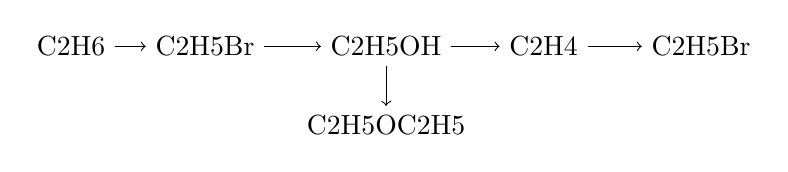
\begin{tikzpicture}
    \node(a)at (0,0) {\ce{C2H6}};
    \node(b)at (1.7,0) {\ce{C2H5Br}};
    \node(c)at (4,0) {\ce{C2H5OH}};
    \node(d)at (6,0) {\ce{C2H4}};
    \node(e)at (8,0) {\ce{C2H5Br}};
    \node(f)at (4,-1) {\ce{C2H5OC2H5}};
    \draw[->](a)--(b);
    \draw[->](b)--(c);
    \draw[->](c)--(d);
    \draw[->](d)--(e);
    \draw[->](c)--(f);
  \end{tikzpicture}\]
  \item 需要多少体积的空气（在标准状况下）才能使 \qty{23}{g} 乙醇完全燃烧？燃烧的结果能生成水和二氧化碳各多少摩尔？放出多少热量？
  \item 写出下列物质的名称，并回答它们是不是同系物？是不是同分异构体？
  \begin{tasks}(2)
    \task \ce{CH3CH2-O-CH2CH3}
    \task \ce{CH3CH2CH2CH2OH}
  \end{tasks}
  \item 某饱和一元醇 \qty{0.3}{g}，跟足量的钠起反应后，生成 \qty{56}{ml} 氢气（标准状况下），求这种一元醇的式量和化学式，并写出这种一元醇可能有的各种同分异构体的结构式和名称。
\end{question}
\end{Practice}

\section{苯酚}
跟链烃有羟基衍生物一样，芳香烃也有羟基衍生物。
在这些化合物里，羟基可以位于侧链的碳原子上，也可以直接连在苯环的碳原子上。
在芳香烃的侧链上含有羟基的衍生物叫做芳香醇，如苯甲醇（\ce{C6H5CH2OH}）。
\emph{羟基跟苯环直接相连的化合物叫做}\Concept{酚}。
苯分子里只有一个氢原子被羟基取代所得的生成物是最简单的酚，叫做苯酚，通常就简称为酚（\cref{fig:3-4}），苯酚的化学式是 \ce{C6H6O}，它的结构式是：
\[ \chemfig{HC*6(=C(-[:-90,0.5,,,draw=none]H)-CH=CH-C(-[:90]OH)=HC-[,,2])} \quad \text{简写为} \quad \chemfig{*6(=-=-(-[:90]OH)=-)} \quad \text{或} \ce{C6H5OH}\]

\begin{figure}
  \includegraphics{3-4.pdf}
  \caption{苯酚分子的比例模型}\label{fig:3-4}
\end{figure}

\subsection{苯酚的性质和用途}
\subsubsection{苯酚的物理性质}
纯净的苯酚是没有颜色的晶体，具有特殊气味，熔点是 \qty{43}{\celsius}，露置在空气里会因小部分发生氧化而显粉红色。
常温时，苯酚在水里溶解度不大，当温度高于 \qty{70}{\celsius} 时，能跟水以任意比互溶。
苯酚易溶于乙醇、乙醚等有机溶剂。
苯酚有毒，它的浓溶液对皮肤有强烈的腐蚀性，\emph{使用时要小心，如果不慎沾到皮肤上，应立即用酒精洗涤}。
焦化厂、煤气厂、化工厂、石油化工厂等的工业废水中常含酚类，如不经处理即排出，就会污染水源。
\subsubsection{苯酚的化学性质}
\paragraph{跟碱的反应——苯酚的酸性}\mbox{}\par
\begin{Experiment}
把少量苯酚晶体放入试管里，再加入 \qty{2}{ml} 水，振荡试管，由于苯酚在水里溶解度不大，溶液里出现浑浊。再逐渐滴入 5\% 的氢氧化钠溶液，继续振荡试管，可以看到溶液变为透明澄清。
\end{Experiment}
苯酚和碱反应，生成了易溶于水的苯酚钠。
\[\schemestart 
\chemfig{[:-30]*6(-=-(-OH)=-=)} \+ \ce{NaOH}
\arrow(.mid east--.mid west)
\chemfig{[:-30]*6(-=-(-ONa)=-=)} \+ \ce{H2O}
\schemestop\]

在这个反应中，苯酚显示了酸性，所以苯酚俗称石炭酸。苯酚中的 \ce{O-H} 键在水分子的作用下能够发生电离：
\[\schemestart 
\chemfig{[:-30]*6(-=-(-OH)=-=)} \+ \ce{H2O}
\arrow(.mid east--.mid west){<=>}
\chemfig{[:-30]*6(-=-(-O^{-})=-=)} \+ \ce{H3O+}
\schemestop\]

但是，苯酚的酸性极弱（电离常数 $K=\num{1.28e-10}$），在水溶液中只能电离出少量 \ce{H+}，甚至不能使指示剂变色。如果在苯酚钠的水溶液里通入二氧化碳，就会有苯酚游离出来。
\[\schemestart
\chemfig{[:-30]*6(-=-(-ONa)=-=)} \+ \ce{CO2} \+ \ce{H2O}
\arrow(.mid east--.mid west)
\chemfig{[:-30]*6(-=-(-OH)=-=)} \+ \ce{NaHCO3}
\schemestop\]

这说明苯酚的酸性比碳酸还要弱（碳酸的电离常数 $K_1=\num{4.3e-7}$）。

\begin{Reading}[补充阅读]{}
苯酚分子中羟基的氧原子含有孤对 $p$ 电子，这 $p$ 电子云可以跟苯环的大 $\pi$ 键电子云从侧面有所重叠，使氧原子上的 $p$ 电子云向苯环转移，氢氧原子之间的电子云向氧原子方向转移，羟基中氢原子较易电离，使苯酚显示一定的酸性。
\[ \chemfig{[:-30]*6(-=-(-[@{a,0.5}]@{oo}\charge{90=\:}{O}-@{h}H)=-=)}
\chemmove{\draw[-stealth]([above=3pt]oo.north)to[bend right=60]([above=2pt]a);
\draw[-stealth](h)--(oo);}
\]
\end{Reading}


\paragraph{苯环上的取代反应}\mbox{}\par
苯酚能跟卤素、硝酸、硫酸等发生苯环上的取代反应。
\begin{Experiment}
在盛有少量苯酚溶液的试管中，滴入过量的浓溴水，可以观察到很快有白色沉淀生成。
\end{Experiment}
上述实验说明，向苯酚溶液里加入溴水，既不需要加热，也不用催化剂，立即生成白色的三溴苯酚沉淀。

\[\schemestart
\chemfig{*6(=-=-(-[:90]OH)=-)} \+ \ce{3Br2} 
\arrow(.mid east--.mid west) 
\chemfig{*6(=(-[:-90]Br)-=(-[:0]Br)-(-[:90]OH)=(-[:180]Br)-)}
\ce{ v } \+ \ce{3HBr}
\schemestop\]

这个反应很灵敏，常用于苯酚的定性检验和定量测定。
\paragraph{显色反应}\mbox{}\par
\begin{Experiment}
在盛有苯酚溶液的试管中，滴入几滴 \ce{FeCl3} 溶液，振荡，溶液显紫色。
\end{Experiment}
苯酚跟 \ce{FeCl3} 溶液作用能显示紫色\footnote{苯酚跟 \ce{FeCl3} 在水溶液里起反应，生成络离子而显紫色。\[\ce{6C6H5OH + Fe^3+ -> [Fe(C6H5O)6]^3- + 6H+}\]}。利用这一反应也可以检验苯酚的存在。

\begin{Theorem}{讨论}
比较苯酚和乙醇在分子结构上和性质上有什么相同点和不同点。
\end{Theorem}

\subsubsection{苯酚的用途}
苯酚是一种重要的化工原料，可用来制造酚醛塑料（俗称电木）、合成纤维（如锦纶）、医药、染料、农药等。
粗制的苯酚可用于环境消毒。
纯净的苯酚可配成洗剂和软膏，有杀菌和止痛效用。
药皂中也掺入少量的苯酚。

\subsection{苯酚的工业制法}
过去工业上主要是从煤焦油里提取苯酚的。
随着化工生产的发展，苯酚的需要量越来越大，从煤焦油提取苯酚早已不能满足需要，目前苯酚主要是采用合成法来制取的。
合成苯酚的方法有多种，一般用苯作为原料来合成。
例如，用 \ce{FeCl3} 作催化剂，可使苯氯化制得氯苯；用 \ce{Cu} 作催化剂在高温加压下，氯苯在碱性溶液中可以水解制得苯酚。
\[\schemestart 
\chemfig{[:-30]*6(-=-=-=)} \+ \ce{Cl2} 
\arrow(.mid east--.mid west){->[\scriptsize 催化剂]}
\chemfig{[:-30]*6(-=-(-Cl)=-=)}
\+ 
\ce{HCl}
\schemestop\]
\[\schemestart 
\chemfig{[:-30]*6(-=-(-Cl)=-=)}
\+ 
\ce{H2O}
\arrow(.mid east--.mid west){->[\scriptsize 催化剂][\scriptsize 高温、加压]} 
\chemfig{[:-30]*6(-=-(-OH)=-=)}
\+ 
\ce{HCl}
\schemestop\]

\begin{Practice}[习题]
\begin{question}
  \item 在澄清的苯酚钠溶液里通入二氧化碳，溶液里变得浑浊；再加入氢氧化钠溶液，溶液又会变为澄清，为什么？写出反应的化学方程式。
  \item 从煤焦油里得到了苯酚和苯的同系物的混和物，用什么方法可以把它们分离？
  \item 怎样鉴别乙醇溶液和苯酚溶液？
  \item 某种有机物含碳 76.6\%、氢 6.38\%、氧 17.02\%，它的式量是乙烷的 3.13 倍，求它的化学式。这种有机物的水溶液加氯化铁溶液呈紫色。写出它的结构式和名称。
\end{question}
\end{Practice}

\section{醛和酮}
醛和酮是含有羰\footnote{羰音 \pinyin{tang1}}基的烃的衍生物。羰基是一个碳原子和一个氧原子以双键相连而成的一种原子团（\chemfig{-C(=[:90]O)-}）。如果羰基的碳原子连着一个氢原子，就构成 \chemfig{-C(=[:90]O)-H}，这种原子团叫做醛基。\emph{分子里由烃基跟醛基相连而构成的化合物叫做}\Concept{醛}。醛类的通式是 \chemfig{R-C(=[:90]O)-H}。

\emph{分子里由羰基跟两个烃基相连而构成的化合物，叫做}\Concept{酮}。酮分子里的羰基又可叫做酮基。酮类物质的通式是
\[ \chemfig{R-C(=[:90]O)-R'}\]

\subsection{乙醛}
\subsubsection{乙醛的物理性质}
乙醛是一种没有颜色、具有刺激性气味的液体，比水轻，沸点是 \qty{20.8}{\celsius}。乙醛易挥发，能跟水、乙醇、乙醚、氯仿等互溶。

\par\medskip\noindent
\begin{minipage}{0.6\linewidth}\parindent2em
乙醛（\cref{fig:3-5}）的化学式是 \ce{C2H4O}，它的结构式是：
\[\chemfig{H-C(-[:90]H)(-[:-90]H)-C(=[:90]O)-H}\]
简写为 \chemfig{CH_3-C(=[:90]O)-H} 或 \ce{CH3CHO}。
\end{minipage}\hfill
\begin{minipage}{0.35\linewidth}
\begin{figurehere}
  \includegraphics{3-5.pdf}
  \caption{乙醛分子的比例模型}\label{fig:3-5}
\end{figurehere}
\end{minipage}

\subsubsection{乙醛的化学性质}
乙醛分子中的醛基（\chemfig{-C(=[:90]O)-H}）官能团对乙醛的主要化学性质起决定作用。
\paragraph{加成反应}\mbox{}\par
碳氧双键能够发生加成反应，例如使乙醛蒸气跟氢气的混和物，通过热的镍催化剂时，就发生加成反应，乙醛被还原成乙醇。
\[\schemestart 
\chemfig{CH_3-C(=[:90]O)-H} \+ \ce{H2} 
\arrow(.mid east--.mid west){->[\scriptsize 催化剂][\scriptsize $\triangle$]}
\ce{CH3CH2OH}
\schemestop\chemnameinit{}\]

\begin{Reading}[补充阅读]{}
羰基上的碳氧双键跟烯烃分子里的碳碳双键一样，也是由一个 $\sigma$ 键和一个 $\pi$ 键组成，能够起加成反应。
\[\chemfig{-\charge{-90[anchor=90]={\tiny\chemdelta$+$}}{C}([2]=[@{a,0.5}]@{oo}\charge{135[anchor=-45]={\tiny\chemdelta$-$}}{O})-H}
\chemmove{\draw[-stealth]([right=4pt]a)to[bend right=45]([right=4pt]oo);}
\]

由于羰基里氧原子的电负性大，从而使碳氧双键的电子云，特别是 $\pi$ 键的电子云偏向氧原子。

当极性分子，如 \ce{HCN} 跟羰基起加成反应时，带正电的原子或基团加在氧原子上，带负电的原子或基团加在碳原子上。
\[\schemestart 
\chemfig{CH_3-C(=[:90]O)-H} \+ \ce{HCN} 
\arrow(.mid east--.mid west)
\chemfig{CH_3-C(-[:90]OH)(-[:-90]CN)-H} 
\schemestop\]
\end{Reading}

\paragraph{氧化反应}\mbox{}\par
我们早已知道，氧化—还原反应是从得氧即是氧化，失氧即是还原，开始认识的。
在有机化学的反应里，通常还可以从加氢或去氢来分析，即去氢就是氧化反应，加氢就是还原反应，所以，乙醛加氢就是乙醛被还原。
乙醛还能够被弱氧化剂所氧化。
\begin{Experiment}
在洁净的试管里加入 \qty{1}{ml} 2\% 的 \ce{AgNO3} 溶液，然后一边摇动试管，一边逐渐滴入 2\% 的稀氨水，直到最初产生的沉淀恰好溶解为止（这时得到的溶液通常叫做银氨溶液）。然后再加入 3 滴乙醛，振荡后，把试管放在热水浴里温热。不久，可以观察到试管内壁上会附着一层光亮如镜的金属银。
\end{Experiment}

在这个反应里，硝酸银跟氨水起反应，生成银氨络合物，它把乙醛氧化成乙酸，乙酸跟氨生成乙酸铵，而银氨络合物的银离子被还原成金属银，附着在试管的内壁上，形成银镜，所以，这个反应叫做\Concept{银镜反应}。
\begin{gather*}
  \ce{ Ag+ + NH3.H2O = AgOH v + NH4+ } \\
  \ce{ AgOH + 2NH3.H2O = [Ag(NH3)2]+ + OH- + 2H2O }
\end{gather*}
\begin{multline*}
    \ce{ CH3CHO + 2[Ag(NH3)2]+ + 2OH- -> \\ 
    CH3COO- + NH4+ + 2Ag v + 3NH3 + H2O}
\end{multline*}

银镜反应常用来检验醛基的存在。
工业上利用这一反应原理，把银均匀地镀在玻璃上制镜或保温瓶胆（生产上常用含有醛基的葡萄糖作为还原剂）。

乙醛也能被另一种弱氧化剂，即新制的氢氧化铜所氧化。
\begin{Experiment}
在试管里加入 10\% \ce{NaOH} 溶液 \qty{2}{ml}，滴入 2\% \ce{CuSO4} 溶液 \numrange{4}{6} 滴，振荡。然后加入乙醛溶液 \qty{0.5}{ml}，加热到沸腾。观察溶液中有红色沉淀产生。
\end{Experiment}
由于乙醛具有还原性，所以能把反应中生成的氢氧化铜还原成红色的氧化亚铜沉淀。
这也是检验醛基的一种方法。
\begin{gather*} 
  \ce{ Cu^2+ + 2OH- =Cu(OH)2 v }\\ 
  \ce{CH3CHO + 2Cu(OH)2 ->[\triangle] CH3COOH + Cu2O v +2H2O}
\end{gather*}

\subsubsection{乙醛的用途}
乙醛是有机合成工业中的重要原料，主要用来生产乙酸、丁醇等。
例如，工业上，乙醛在一定温度和催化剂条件下，被空气氧化生成乙酸。
\[\schemestart 
\ce{2CH3CHO} \+ \ce{O2} \arrow(.mid east--.mid west){->[\scriptsize 催化剂]}
\chemname{\ce{2CH3COOH}}{\footnotesize 乙酸}
\schemestop\chemnameinit{}\]

\subsubsection{乙醛的工业制法}
乙醛最早是采用乙醇氧化法制得的，这种方法需要耗用大量粮食，后来又采用了乙炔水化法。
近年来，随着石油化工的发展，又创造了乙烯氧化法制乙醛的新技术。
\paragraph{乙炔水化法}\mbox{}\par
用汞盐（如 \ce{HgSO4}）作催化剂，乙炔跟水化合，生成乙醛。
\[ \ce{ CH#CH +  H2O ->[\text{催化剂}] CH3CHO }\]

这个方法生产的乙醛纯度较高，但操作人员在生产中容易发生汞中毒。
目前正在研究以非汞催化剂代替汞催化剂，并已取得初步成效。

\paragraph{乙烯氧化法}\mbox{}\par
在一定温度和压强下，用氯化钯（\ce{PdCl2}）和氯化铜（\ce{CuCl2}） 作催化剂，使乙烯被空气或氧气直接氧化成乙醛。
\[ \ce{ 2CH2=CH2 +  O2 ->[\text{催化剂}][\text{加热、加压}] 2CH3CHO }\]

乙烯可以由石油裂化气中取得。
用乙烯氧化法生产乙醛，流程简单，原料丰富，成本低，产率高。

\subsection{醛类}
除乙醛外，还有一些在分子结构上和化学性质上都跟乙醛相似的物质，如甲醛（\ce{HCHO}）、丙醛（\ce{CH3CH2CHO}）等。
由于醛类分子里都含有醛基，所以它们的化学性质很相似。
例如，它们都能被还原为醇，被氧化为酸，都能起银镜反应等。

在醛类中，甲醛也有广泛的用途。
甲醛也叫蚁醛，是一种无色具有强烈刺激性气味的气体，易溶于水，35\%～40\% 的甲醛水溶液叫做福尔马林。
甲醛是一种重要的有机原料，应用于塑料工业（如制酚醛树脂）、合成纤维工业、制革工业等。甲醛的水溶液具有杀菌和防腐能力，是一种良好的杀菌剂。
在农业上常用稀福尔马林溶液（0.1\%～0.5\%）来浸种，给种子消毒。
福尔马林还用来浸制生物标本。

酚醛树脂是最早生产和使用的合成树脂，由于它不易燃烧并有良好的电绝缘性能，至今还用作电木（一种塑料）的原料。

酚醛树脂通常用苯酚跟甲醛起反应而制得。这个反应可简单地表示如下：
\[\schemestart
$n$\,\chemfig{*6(=-=-(-OH)=-)} \+ $n$\chemfig{HCH=[:90,,2]O} \arrow(.mid east--.mid west)
\chemfig{*6(=-=(-[:0]CH_2-[@{cl,0.4}:0])-(-OH)=(-[@{op,0.6}:180])-)}
\polymerdelim[delimiters ={[]},depth=30pt,indice =\!n]{op}{cl}
\+ $n$\,\ce{H2O}
\schemestop\]

单体间相互反应而成高分子化合物，同时还生成小分子（如水、氨等）的反应叫做\Concept{缩聚反应}。

\subsection{丙酮}
丙酮是一种没有颜色、有气味的液体，沸点是 \qty{56.2}{\celsius}，密度是 \qty{0.7899}{g/cm^3}，易挥发，易燃烧。它可跟水、乙醇及乙醚等以任意比互溶。丙酮还能够溶解脂肪、树脂和橡胶等很多有机物，它是一种重要的有机溶剂。
\par\medskip\noindent
\begin{minipage}{0.6\linewidth}\parindent2em
丙酮（\cref{fig:3-6}）的化学式是 \ce{C3H6O}，它的结构式是
\[\chemfig{CH_3-C(=[:90]O)-CH_3}\]
简写为 \ce{CH3COCH3}。
\end{minipage}\hfill
\begin{minipage}{0.35\linewidth}
\begin{figurehere}
  \includegraphics{3-6.pdf}
  \caption{丙酮分子的比例模型}\label{fig:3-6}
\end{figurehere}
\end{minipage}\par\medskip

丙酮没有还原性，不跟银氨溶液起银镜反应。在催化剂（\ce{Ni}、\ce{Co}、\ce{Pt}、\ce{Pd} 等）存在的条件下，可以跟氢气起加成反应，生成醇。

\begin{Practice}[习题]
\begin{question}
  \item 下列哪些物质可以发生银镜反应？
  \begin{tasks}(4)
    \task  甲醛
    \task  乙醇
    \task* 葡萄糖（\ce{CH2OH(CHOH)4CHO}）
  \end{tasks}
  \item 某种醛的组成是含碳 62.1\%、氢 10.3\%、氧 27.6\%，它的蒸气密度是氢气的 29 倍。写出这种醛的化学式、结构式和名称。
  \item 分别写出以石油或焦炭为原料生产乙醛的有关化学方程式。
  \item 醛和酮在分子结构上有什么相同处和不同处？在性质上有什么重要区别？如何用化学方法鉴别乙醛和丙酮？
  \item 分子里含有碳、氢、氧三种元素的烃类衍生物，已学过的有醇、醚、醛、酮等类，假定它们分子里都含有 3 个碳原子，写出各类物质的结构式，说出名称，并指出哪些互为同分异构体？
\end{question}
\end{Practice}

\section{乙酸}
乙酸（\ce{CH3COOH}）是一种重要的有机酸，它是食醋的主要成分，普通的食醋中含有 3\%～5\% 的乙酸，所以乙酸又叫醋酸。
\par\medskip\noindent
\begin{minipage}{0.6\linewidth}\parindent2em
乙酸（\cref{fig:3-7}）的化学式是 \ce{C2H4O2}，它的结构式是：\chemfig{CH_3-[,0.8]C(=[:90,0.8]O)-[,0.8]OH}，简写为 \ce{CH3COOH}。

乙酸分子里的 \chemfig{-[,0.8]C(=[:90,0.8]O)-[,0.8]OH}（或\ce{-COOH}）官能团叫做羧基，它是由羰基（\chemfig{C(-[:135,0.8])(-[:225,0.8])=O}）和羟基（\ce{-OH}）组成的。
\end{minipage}\hfill
\begin{minipage}{0.35\linewidth}
\begin{figurehere}
  \includegraphics{3-7.pdf}
  \caption{乙酸分子的比例模型}\label{fig:3-7}
\end{figurehere}
\end{minipage}

\subsection{乙酸的性质}
\subsubsection{乙酸的物理性质}
乙酸是一种有强烈刺激性气味的无色液体，沸点是 \qty{117.9}{\celsius}，熔点是 \qty{16.6}{\celsius}，当温度低于 \qty{16.6}{\celsius} 时，乙酸就凝结成象冰一样的晶体，所以无水乙酸又称冰醋酸。
乙酸易溶于水和乙醇。

\subsubsection{乙酸的化学性质}
\paragraph{酸性}\mbox{}\par
乙酸具有明显的酸性，在水溶液里能电离出氢离子。
\[ \ce{ CH3COOH <=> CH3COO- + H+ }\]

乙酸是一种弱酸，它的电离常数 $K=\num{1.75e-5}$，但比碳酸的酸性强，它具有酸的通性。

\begin{Reading}[补充阅读]{}\par\medskip\noindent
\begin{minipage}{0.75\linewidth}\parindent2em
羧基里的羰基跟醛基里的羰基相似，也是由一个 $\sigma$ 键和一个 $\pi$ 键组成，碳氧键的电子云偏向氧原子。羟基里的氧原子含有孤对 $p$ 电子，这 $p$ 电子云可以跟羰基的 $\pi$ 电子云从侧面有所重叠，使羟基氧原子的电子云向羰基转移，氢氧原子间的电子云向氧原子转移，使氢原子能够电离，具有羧基的乙酸等显示酸性。
\end{minipage}\hfill
\begin{minipage}{0.23\linewidth}
\[\chemfig{-C([2]=[@{a1,0.5}]@{o1}O)-[@{a2,0.5}]@{o2}\charge{90=\:}{O}-H}
\chemmove{\draw[-stealth]([xshift=4pt]a1)to[bend right=60]([xshift=4pt]o1);\draw[-stealth]([yshift=4pt]o2.north)to[bend right=60]([yshift=2pt]a2);}
\]
\end{minipage}
\end{Reading}

\paragraph{酯化反应}\mbox{}\par
在有浓硫酸存在并加热的条件下，乙酸能够跟乙醇发生反应，生成乙酸乙酯。
\begin{Experiment}
在试管里先加入 \qty{3}{ml} 乙醇，然后一边摇动，一边慢慢地加入 \qty{2}{ml} 浓硫酸和 \qty{2}{ml} 冰醋酸。按\cref{fig:3-8} 装置好。用酒精灯小心均匀地加热试管 \qtyrange{3}{5}{min}。产生的蒸气经导管通到饱和碳酸钠溶液的液面上。在液面上可以看到有透明的油状液体生成，并可闻到一种香味。
\tcblower
\begin{figurehere}
  \includegraphics{3-8.pdf}
  \caption{乙酸乙酯的制备}\label{fig:3-8}
\end{figurehere}
\end{Experiment}

这种有香味的无色透明油状液体就是乙酸乙酯。
由于反应生成的乙酸乙酯在同样的条件下，又能部分地发生水解反应，生成乙酸和乙醇。
所以上述反应实际上是可逆的。
\[\schemestart 
\chemfig{CH_3-C(=[:90]O)-OH}\tikz[remember picture]\coordinate(a); \+ \tikz[remember picture]\coordinate(b); \chemfig{H-^{18}O-C_2H_5}
\arrow(.mid east--.mid west){<=>[\footnotesize 浓 \ce{H2SO4}][\footnotesize $\triangle$]}
\chemfig{CH_3-C(=[:90]O)-^{18}OC_2H_5} + \ce{H2O}
\schemestop\chemnameinit{}
\tikz[overlay,remember picture]{\draw[densely dashed]([xshift=-2em,yshift=-1ex]a)rectangle([xshift=1.5em,yshift=2.5ex]b);}\]

如果用含氧的同位素 \ce{^{18}_8O} 的乙醇跟乙酸起反应时，就发现乙酸乙酯分子里含有 \ce{^{18}_8O} 原子。所以酯化反应的过程一般是：羧酸分子中的羟基跟醇分子中的氢原子结合成水，其余部分互相结合成酯。

乙酸乙酯是属于酯类化合物的一种。
\emph{酸跟醇起作用，生成酯和水的反应叫做}\Concept{酯化反应}。

\subsection{乙酸的用途}
乙酸是一种重要的有机化工原料，用途很广泛，可用于生产醋酸纤维、合成纤维（如维纶）、喷漆溶剂、增塑剂、香料、染料、医药（如阿斯匹林） 以及农药等。
\subsection{乙酸的制法}
工业上制取乙酸的方法有多种。
过去用发产法制乙酸，即用含糖类物质发酵制乙醇，乙醇经过发酵被氧化成乙醛，乙醛进一步被氧化，即制得乙酸。
食醋就是这样制取的。
目前大都采用乙烯氧化法，较新的是烷烃直接氧化法。

\subsubsection{乙烯氧化法}
乙烯氧化法生产乙酸的原理是使乙烯在有催化剂如氯化钯（\ce{PdCl2}）和氯化铜（\ce{CuCl2}）存在的条件下，跟氧发生反应，生成乙醛。
乙醛再在催化剂如醋酸锰（\ce{(CH3COO)2Mn}）的作用下，被氧化生成乙酸。
\begin{align*}
  \ce{ 2CH2=CH2 + O2 } & \ce{ ->[\text{催化剂}] 2CH3CHO }\\
  \ce{ 2CH3CHO + O2 } & \ce{ ->[\text{催化剂}] 2CH3COOH }
\end{align*}
这种方法的原料是乙烯，可以从石油加工产品中获得，因此来源很丰富。

\subsubsection{烷烃直接氧化法}
直接氧化法又叫丁烷氧化法。
这是近来发展起来的一种新的生产乙酸的方法。
这种方法的主要原料是石油炼制所产生的低沸点烷烃（主要是 \ce{C4}～\ce{C6} 馏分），这些低沸点烷烃在一定的温度、压强和催化剂（如羧酸的钴盐等）存在的条件下，被空气中的氧气直接氧化，生成乙酸。
\[ \ce{ 2CH3CH2CH2CH3 + 5O2 ->[\text{催化剂}][\text{加温、加压}] 4CH3COOH + 2H2O }\]



\begin{Practice}[习题]
\begin{question}
  \item 写出乙酸跟下列物质起反应的化学方程式：
  \begin{tasks}(3)
    \task 金属镁，
    \task 生石灰，
    \task 苛性钠溶液，
    \task 纯碱溶液，
    \task 甲醇。
  \end{tasks}
  \item 怎样用化学方法区别乙醇、乙醛和乙酸三种物质的水溶液？
  \item \qty{10}{g} 水和 \qty{40}{g} 乙酸混和配成乙酸溶液，它的密度是 \qty{1.07}{g/cm^3}，求该乙酸溶液的摩尔浓度。
  \item 用 \qty{30}{g} 乙酸和 \qty{46}{g} 乙醇反应，如果实际产率是理论产率的 85\%，可以得到多少克乙酸乙酯？
  \item 写出以水、空气和乙烯为原料制取乙酸乙酯的各步反应的化学方程式。
\end{question}
\end{Practice}


\section{羧酸}
在有机化合物里，有一大类化合物，它们跟乙酸相似，分子里都含有羧基官能团，因而它们具有跟乙酸相似的化学性质，如有酸性，能发生酯化反应等。

\begin{table}
  \caption{几种羧酸的沸点和电离常数}\label{tab:3-2}
  \begin{tblr}{colspec={X[c]X[2,r]S[table-format=6.2]c},hline{2}=0.8pt,row{1}={m,c,guard}}
    名称 & 结构简式 & 沸点（\unit{\celsius}）& $K$ \\
    甲酸   & \chemfig{H-C(=[:90]O)-OH}              & 100.7 & \num{1.77e-4} \\
    乙酸   & \chemfig{CH_3-C(=[:90]O)-OH}           & 117.9 & \num{1.75e-5} \\
    丙酸   & \chemfig{CH_3-CH_2-C(=[:90]O)-OH}      & 140.99 & \num{1.34e-5} \\
    丁酸   & \chemfig{CH_3-CH_2-CH_2-C(=[:90]O)-OH} & 163.5 & \num{1.54e-5} \\
    苯甲酸 & \chemfig{C_6H_5-C(=[:90]O)-OH}         & 249 & \num{6.46e-5} \\
  \end{tblr}
\end{table}

\cref{tab:3-2} 里各种羧酸的分子里，跟羧基直接相连的烃基不同，所以它们的性质又有所不同。

这类\emph{在分子里烃基跟羧基直接相连接的有机化合物叫做}\Concept{羧酸}。
根据羧基所连接的烃基不同，羧酸可以分为脂肪酸（如乙酸）和芳香酸 （如苯甲酸 \ce{C6H5-COOH}）。
此外也可以根据羧酸分子中含有羧基数目来分类，含有一个羧基的叫一元羧酸，如甲酸、乙酸等；含有两个羧基的叫做二元羧酸，如乙二酸（\ce{HOOC-COOH}）、己二酸（\ce{HOOC(CH2)4COOH}）等。

一元羧酸的通式为 \ce{R-COOH}。下面介绍一些重要的羧酸。

\subsection{甲酸}
甲酸（\ce{HCOOH}）俗称蚁酸。它是无色、有刺激性气味的液体，有腐蚀性，能跟水混溶。

\par\medskip\noindent
\begin{minipage}{0.7\linewidth}\parindent2em
甲酸是羧酸里最简单的一种酸。
它的结构跟其它羧酸不同，在甲酸的分子中，跟羧基相连的不是烃基，而是氢原子。
它既具有羧基的结构（虚线圆圈内为羧基），又具有醛基的结构（方框内为醛基）。
甲酸这种结构上的特殊性，使得它既表现出羧酸的性质，又表现出醛的性质。
例如，甲酸既具有酸的通性，又有还原性。
甲酸能使银氨络离子还原为金属银，而本身被氧化为二氧化碳和水。
\end{minipage}\hfill
\begin{minipage}{0.25\linewidth}
  \centering\includegraphics{3-a.pdf}
\end{minipage}
\par\medskip

甲酸在工业上主要用作还原剂、印染工业上的媒染剂、医药上的消毒剂等。

\subsection{高级脂肪酸}
在一元羧酸里，有些酸分子的烃基含有较多的碳原子，我们把烃基里含碳原子比较多的脂肪酸叫做\Concept{高级脂肪酸}。
例如硬脂酸（\ce{C17H35COOH}）、软脂酸（\ce{C15H31COOH}）和油酸 （\ce{C17H33COOH}）等都是重要的高级脂肪酸。
其中油酸的烃基里含有一个双键，而硬脂酸和软脂酸的烃基里没有不饱和键。 
硬脂酸、软脂酸属于饱和高级脂肪酸，常温下呈固态。
油酸属于不饱和高级脂肪酸，常温下呈液态。
高级脂肪酸不溶于水。
\begin{enumerate}[1.]
  \item 高级脂肪酸分子中含有羧基，所以具有羧酸的性质。如高级脂肪酸能够跟碱溶液反应而生成盐。
  \[\schemestart
  \chemname{\ce{C17H35COOH}}{\footnotesize 硬脂酸} \+ \ce{NaOH} 
  \arrow(.mid east--.mid west)
  \chemname{\ce{C17H35COONa}}{\footnotesize 硬脂酸钠} \+ \ce{H2O}
  \schemestop\chemnameinit{}\]

  我们日常使用的肥皂的主要成分就是高级脂肪酸的钠盐。
  \item 油酸分子中有一个不饱和双键，所以油酸除了能发生上述反应外，还可以跟氢气或氯气发生加成反应。例如，液态的油酸在金属镍作催化剂的条件下，跟氢气起加成反应，就能生成固态的硬脂酸。
  \[ \ce{ C17H33COOH + H2 ->[\text{催化剂}][\triangle] C17H35COOH }\]
\end{enumerate}

\subsection{苯甲酸}
苯甲酸（\ce{C6H5-COOH}）俗名安息香酸，是属于芳香酸类的有机化合物。
它是芳香酸中分子组成最简单的一种酸。
苯甲酸是一种白色针状晶体，熔点是 \qty{122.4}{\celsius}，易升华，微溶干水，易溶于乙醇、乙醚。
苯甲酸的酸性比乙酸稍强一点。
苯甲酸是有机合成的原料，除了可以制香料外，还用来制造染料、药物等。
它的钠盐可作食物的防腐剂。

\subsection{乙二酸}
乙二酸（\ce{HOOC-COOH}）俗名草酸。
它是一个最简单的二元羧酸。
草酸是没有颜色的透明晶体。
通常含有两个分子结晶水，能溶于水或乙醇。
草酸是一种重要的化工原料，可用作还原剂和用于提炼稀有金属等。

\begin{Practice}[习题]
\begin{question}
  \item 什么叫做羧酸？羧酸的官能团是什么？它具有哪些化学性质？
  \item 甲酸水溶液能不能跟碳酸钠起反应，能不能跟银氨络离子起反应？为什么？
  \item 最简单的不饱和酸是丙烯酸（\ce{CH2=CH-COOH}）。丙烯酸能起哪些反应？并写出反应的化学方程式。
  \item 甲酸俗名蚁酸。因为蚂蚁和蜂等很多昆虫的分泌液里都含有甲酸。当我们被蜂等叮咬后，涂上一点稀氨水或稀碳酸钠溶液就可以止痒止痛，这是为什么？试写出反应的化学方程式。
  \item 怎样用化学方法鉴别以下各组物质？
  \begin{tasks}[label=(\arabic*)](2)
    \task 甲醛、甲酸和乙酸，
    \task 甲醇、甲酸和丙酸。
  \end{tasks}
\end{question}
\end{Practice}

\section{酯}
我们学过，乙酸和乙醇在有浓硫酸存在的条件下，能够发生反应，生成乙酸乙酯。同样，其它的酸也可以跟醇发生类似的反应。如甲酸跟乙醇在浓硫酸存在的条件下发生反应，生成甲酸乙酯。
\[\schemestart
\chemfig{H-COOH} \+ \chemfig{HO-C_2H_5}
\arrow(.mid east--.mid west){->[\scriptsize 浓 \ce{H2SO4}]}
\chemname{\ce{HCOOC2H5}}{\footnotesize 甲酸乙酯}
\+ \ce{H2O} 
\schemestop\chemnameinit{}\]

\emph{酸跟醇起反应，生成的一类化合物叫做}\Concept{酯}。
酯的一般通式是 \ce{RCOOR$'$}。
其中 \ce{R} 和 \ce{R$'$} 可以相同，也可以不同。
酯类化合物是根据生成酯的酸和醇的名称来命名的。
例如，\ce{CH3COOC2H5} 叫乙酸乙酯，\ce{HCOOCH3} 叫甲酸甲酯。

硝酸等无机酸也能够跟醇起反应，生成的也是酯，如：
\[\schemestart
\chemfig{C_2H_5OH} \+ \chemfig{HO-NO_2}
\arrow(.mid east--.mid west)
\chemname{\ce{HC2H5-NO2}}{\footnotesize 硝酸乙酯}
\+ \ce{H2O} 
\schemestop\chemnameinit{}\]

酯类广泛地存在于自然界里。
低级酯是有芳香气味的液体，存在于各种水果和花草中。
例如，梨里含有乙酸异戊酯，苹果和香蕉里含有异戊酸异戊酯等。
酯一般比水轻，难溶于水，易溶于乙醇和乙醚等有机溶剂。
酯可用作溶剂，并用作制备饮料和糖果的果子香料。

酯的重要化学性质是能够跟水发生水解反应。

\begin{Experiment}
  在三个试管里，各加入 6 滴乙酸乙酯。再向第一个试管里加蒸馏水 \qty{5.5}{ml}。向第二个试管里加稀硫酸（$1:5$）\qty{0.5}{ml}，蒸馏水 \qty{5}{ml}。向第三个试管里加 30\% 氢氧化钠溶液 \qty{0.5}{ml}、蒸馏水 \qty{5}{ml}。振荡均匀后，把三个试管都放入 \qtyrange{70}{80}{\celsius} 的水浴里加热。几分钟后,在第三个试管里，乙酸乙酯的气味就完全消失了。第二个试管里，还剩一点乙酸乙酯的气味。而第一个试管里乙酸乙酯的气味没有多大变化。
\end{Experiment}
实验说明，在有酸和碱存在的条件下，酯类跟水发生水解反应，生成相应的酸和醇。例如，乙酸乙酯水解后生成乙酸和乙醇。
\[\schemestart
\ce{CH3COOC2H5} \+ \ce{H2O}
\arrow(.mid east--.mid west){<=>[\scriptsize 无机酸或碱]}
\ce{CH3COOH} \+ \ce{C2H5OH} 
\schemestop\chemnameinit{}\]

酯的水解反应是酯化反应的逆反应。当酯化和水解速度相等的时候，混和物中反应处于平衡状态。
\[\schemestart
\ce{RCOOH} \+ \ce{HOR$'$}
\arrow(.mid east--.mid west){<=>[\scriptsize 酯化][\scriptsize 水解]}
\ce{RCOOR$'$} \+ \ce{H2O} 
\schemestop\chemnameinit{}\]

处于平衡状态时，酯类水解的程度跟反应条件有密切关系。
当有碱存在时，碱跟水解生成的酸发生中和反应，此时水解程度就大。
\[ \ce{ ROOH + NaOH -> RCOONa + H2O }\]
当只有无机酸存在时，它只起催化作用但不能减少水解生成的酸，水解的程度就小。

在实际生产中，可以根据需要，控制一定的条件，使反应向所需要的方向进行，如可以加碱以促进酯的水解。

\begin{Practice}[习题]
\begin{question}
  \item 写出下列物质的结构简式。
  \begin{tasks}[label=(\arabic*)](4)
    \task 丁酸乙酯，
    \task 丙酸甲酯，
    \task 丁酸辛酯，
    \task 苯甲酸乙酯。
  \end{tasks}
  \item 写出甲酸跟下列物质起反应的化学方程式，并说明怎样实现这两个反应。
  \begin{tasks}[label=(\arabic*)](2)
    \task 甲醇，
    \task 乙醇。
  \end{tasks}
  \item 哪种羧酸或酯的组成是 \ce{C3H6O2}？写出它们的结构式和名称。
  \item 怎样实现下列反应？写出有关的化学方程式。
  \begin{tasks}[label=(\arabic*)]
    \task \ce{C}$\to$\ce{CaC2}$\to$\ce{C2H2}$\to$\ce{CH3CHO}$\to$\ce{CH3COOH}$\to$\ce{CH3COOC2H5}，
    \task \ce{CH3OH}$\to$\ce{HCHO}$\to$\ce{HCOOH}$\to$\ce{HCOOC2H5}。
  \end{tasks}
  \item 某有机物的蒸气密度是空气的 3.04 倍，该有机物 \qty{2.2}{g} 燃烧后得到 \qty{1.8}{g} 水及 \qty{2.24}{L}二氧化碳（标准状况下），求该有机物的化学式。如果该有机物能发生银镜反应，并能水解生成醇和酸，试确定它的结构式，并写出有关的化学方程式。
\end{question}
\end{Practice}

\section{油脂}
油脂是人类的主要食物之一，也是一种重要的工业原料。
我们日常食用的猪油、牛油、羊油、花生油、菜籽油、豆油、棉籽油等都是油脂。

在通常的温度下，油脂有呈固态的，也有呈液态的。
一般说来，呈固态的叫做脂肪，呈液态的叫做油。
因为植物油脂通常呈液态，叫做油。
动物油脂通常呈固态，叫做脂肪。
脂肪和油统称油脂。
它们在化学成分上都是高级脂肪酸跟甘油所生成的酯，所以油脂属于酯类。

\subsection{油脂的组成和结构}
油脂是由多种高级脂肪酸如硬脂酸、软脂酸或油酸等跟甘油生成的甘油酯。它们的结构可以表示如下：
\[\chemfig{R_2-C(=[:90,0.8]O)-O-CH(-[:90,1.5]CH_2-[:180]O-[:180]C(=[:90,0.8]O)-[:180]R_1)(-[:-90,1.5]CH_2-[:180]O-[:180]C(=[:90,0.8]O)-[:180]R_3)}
\]

结构式里 \ce{R1}、\ce{R2}、\ce{R3} 代表饱和烃基或不饱和烃基。
它们可以相同，也可以不相同。
如果 \ce{R1}、\ce{R2}、\ce{R3} 相同，这样的油脂称为单甘油酯。
如果 \ce{R1}、\ce{R2}、\ce{R3} 不相同，就称为混甘油酯。
天然油脂大都为混甘油酯。

形成油脂的脂肪酸的饱和程度，对油脂的熔点有着重要的影响。
由饱和的硬脂酸或软脂酸生成的甘油酯熔点较高，呈固态。
而由不饱和的油酸生成的甘油酯熔点较低，呈液态。
由于各类油脂中所含的饱和烃基和不饱和烃基的相对量不同，因此，具有不同的熔点。

\subsection{油脂的性质}
\subsubsection{物理性质}
油脂比水轻，密度在 \qtyrange{0.9}{0.95}{g/cm^3} 之间。不溶于水，易溶于汽油、乙醚、苯等多种有机溶剂中。 在工业上，根据这一性质，可用有机溶剂来提取植物种子里的油。

\subsubsection{化学性质}
由于油脂是多种高级脂肪酸的甘油酯的混和物，而高级脂肪酸中，既有饱和的，又有不饱和的。
因此油脂兼有酯类和烯烃的一些化学性质。
\paragraph{油脂的氢化}\mbox{}\par
液态油在催化剂（如 \ce{Ni}）存在下，加热、加压可以跟氢起加成反应，提高油脂的饱和程度，生成固态的油脂。
\[\schemestart 
\chemname{\chemfig{C_{17}H_{33}COO-CH(-[:90]CH_2-[:180]C_{17}H_{33}COO)(-[:-90]CH_2-[:180]C_{17}H_{33}COO)}}{\footnotesize 油酸甘油酯（油）}
\+ \ce{3H2}
\arrow(.mid east--.mid west){->[\scriptsize 催化剂][\scriptsize 加热、加压]}
\chemname{\chemfig{C_{17}H_{35}COO-CH(-[:90]CH_2-[:180]C_{17}H_{35}COO)(-[:-90]CH_2-[:180]C_{17}H_{35}COO)}}{\footnotesize 硬脂酸甘油酯（脂肪）}
\schemestop\chemnameinit{}\]

这个反应叫做油脂的氢化，也叫油脂的硬化。
这样制得的油脂叫人造脂肪，通常又叫硬化油。
工业上常利用油脂的氢化反应把多种植物油转变成硬化油。
硬化油性质稳定、不易变质、便于运输，可用作制造肥皂、脂肪酸、甘油、人造奶油等的原料。

\paragraph{油脂的水解}\mbox{}\par
跟酯类的水解反应相同，在适当的条件下（如有酸或碱或高温水蒸气存在），油脂跟水能够发生水解反应，生成甘油和相应的高级脂肪酸。
例如，硬脂酸甘油酯在有酸存在的条件下进行的水解反应，可以表示如下：
\[\schemestart 
\chemname{\chemfig{C_{17}H_{35}COO-CH(-[:90]CH_2-[:180]C_{17}H_{35}COO)(-[:-90]CH_2-[:180]C_{17}H_{35}COO)}}{\footnotesize 硬脂酸甘油酯}
\+ \ce{3H2O}
\arrow(.mid east--.mid west){<=>[\scriptsize \ce{H2SO4}][\scriptsize $\triangle$]}
\chemname{\ce{3C17H35COOH}}{\footnotesize 硬脂酸} \+ 
\chemname{\chemfig{CH(-[:90]CH_2-OH)(-[:-90]CH_2-OH)-OH}}{\footnotesize 甘油}
\schemestop\chemnameinit{}\]

工业上根据这一反应原理，可用油脂为原料来制取高级脂肪酸和甘油。

如果油脂的水解反应，是在有碱存在的条件下进行的，那么，水解生成的高级脂肪酸便跟碱反应，生成高级脂肪酸盐。
例如硬脂酸甘油酯在有氢氧化钠存在的条件下，发生水解反应，生成硬脂酸钠和甘油。
\[\schemestart
\chemname{\chemfig{C_{17}H_{35}COO-CH(-[:90]CH_2-[:180]C_{17}H_{35}COO)(-[:-90]CH_2-[:180]C_{17}H_{35}COO)}}{\footnotesize 硬脂酸甘油酯}
\+ \ce{3NaOH}
\arrow(.mid east--.mid west)
\chemname{\ce{3C17H35COONa}}{\footnotesize 硬脂酸钠} \+ 
\chemname{\chemfig{CH(-[:90]CH_2-OH)(-[:-90]CH_2-OH)-OH}}{\footnotesize 甘油}
\schemestop\chemnameinit{}\]

油脂在碱性条件下的水解反应也叫\Concept{皂化反应}。

工业上就是利用皂化反应来制造肥皂。
首先把动物性脂肪（牛脂、羊脂等）、植物油（棉籽油、豆油等）和氢氧化钠溶液按一定比放在皂化锅内，用蒸气加热，同时适当搅拌。
因为有过量的碱存在，所以油脂便发生水解反应，生成高级脂肪酸的钠盐和甘油。

反应完成后，生成的高级脂肪酸钠、甘油和水形成混和液。
高级脂肪酸钠在水里形成胶体溶液，为了使肥皂和甘油充分分离，继续加热搅拌，并向锅内慢慢加入食盐细粒。
在电解质的作用下，胶体溶液被破坏，高级脂肪酸钠从混和液中析出。
这个加入食盐使肥皂析出的过程就是盐析。
此时，停止加热和搅拌，静置一定时间，溶液便分上下两层。
上层是高级脂肪酸钠，下层是甘油和食盐的混和液。
取出上层的物质，加入填充剂（如松香和硅酸钠）等，进行压滤、干燥、成型，就制成了成品肥皂。
下层溶液经分离提纯后，便得到甘油。

油脂是一种重要的营养物质,它在完全氧化（生成 \ce{CO2} 和 \ce{H2O} 时放出的热量（约 \qty{9.4}{kCal/g}）要比碳水化合物（约 \qty{4.1}{kCal/g}）放出的热量大得多。
油脂在小肠里的酶（具有催化作用的蛋白质）的作用下，发生水解，主要生成物是脂肪酸和甘油，还有些中间产物。
肠壁能吸收脂肪酸和甘油。
在肠壁细胞里，水解生成物又重新反应生成油脂。
这种油脂经由淋巴液系统到血液里，并随血液的循环进入人体各组织里进行氧化。

\begin{Reading}{去污作用和合成洗涤剂}
  \subparagraph{肥皂的去污作用}\mbox{}\par
  普通的肥皂约含 \({70}\%\) 的高级脂肪酸的钠盐，\({30}\%\) 的水和少量的盐。
  有些肥皂内还加有填充剂、香料及染料等。
  肥皂的去污作用主要是高级脂肪酸的钠盐的作用。
  从结构上看，高级脂肪酸钠的分子可以分为两部分，一部分是极性的 \ce{-COONa} 或 \ce{-COO^-}，这一部分可溶于水，叫做亲水基。另一部分是非极性的链状的烃基 \ce{-R}，这一部分在结构上跟水的差别很大，不能溶于水，叫做憎水基。憎水基具有亲油的性质。在洗涤的过程中，污垢中的油脂跟肥皂接触后，高级脂肪酸钠分子的烃基就插入油滴内。而易溶于水的羧基部分伸在油滴外面，插入水中。这样油滴就被肥皂分子包围起来（\cref{fig:3-9}）。再经摩擦、振动，大的油滴便分散成小的油珠，最后脱离被洗的纤维织品，而分散到水中形成乳浊液，从而达到洗涤的目的。

  \begin{figurehere}
    \includegraphics{3-9.pdf}\par
    {\footnotesize
      \begin{enumerate*}[1.]
      \item 亲水基
      \item 憎水基
      \item 油污
      \item 纤维织品
    \end{enumerate*}}
    \caption{肥皂去污示意图}\label{fig:3-9}
  \end{figurehere}

  \subparagraph{合成洗涤剂}\mbox{}\par
  根据对肥皂去污原理的研究，人们认识到凡是分子的两端分别具有亲水基和憎水基的物质都有一定的去污能力。
  因此，可以利用人工合成的方法来合成具有这种结构的物质作为洗涤剂。
  这就是人们日常所用的合成洗涤剂。
  目前，常用的合成洗涤剂的主要成分是烷基苯磺酸钠或烷基磺酸钠。它们的结构式分别是 \raisebox{1ex}{\chemfig[atom sep=0.7em]{-[,1.7]R-[,1.7]*6(=-=(-[,1.7]SO_3Na)-=-)}} 和 \ce{R-SO3Na}（\cref{fig:3-10}）。其中亲水基都是极性基团 \ce{-SO3Na}，憎水基分别是非极性基团 \raisebox{1ex}{\chemfig[atom sep=0.7em]{-[,1.7]R-[,1.7]*6(=-=(-)-=-)}} 和 \ce{R-{}}。式中 \ce{R} 一般是含十个以上碳原子的烃基。
  烃基含碳原子太少时，憎水作用太弱，使得憎水基跟油的结合力不强。
  相反地，烃基含碳原子太多时，就不容易“溶”于水。
  所以烃基太大或太小都不能很好地达到去污的目的。

  \begin{figurehere}
    \includegraphics{3-10.pdf}
    \caption{合成洗涤剂分子结构示意图}\label{fig:3-10}
  \end{figurehere}

  合成洗涤剂有很强的去污能力。
  湿润、乳化的能力也很强。
  跟肥皂相比，既可以节省大量油脂，它的钙盐和镁盐又能溶于水，因而不受硬水的影响。
  所以，合成洗涤剂的发展很迅速。
\end{Reading}



\begin{Practice}[习题]
\begin{question}
  \item 脂肪和油的区别在哪里？如何把油转化为脂肪？写出反应的化学方程式。
  \item 油脂在什么情况下可以水解？水解后可以得到哪些产物？写出它们的化学方程式。
  \item 各举一例说明下列各化学反应在有机化学工业上的应用，并写出反应的化学方程式。
  \begin{tasks}[label=(\arabic*)](2)
    \task 酯化，
    \task 皂化。
  \end{tasks}
  \item 如果硬脂酸甘油酯水解时，仅有 85\% 的硬脂酸甘油酯起反应，那么要制得 \qty{5}{t} 甘油，需要多少吨硬脂酸甘油酯？
\end{question}
\end{Practice}

\section{硝基化合物}
\emph{烃分子中的氢原子被硝基}（\ce{-NO2}）\emph{取代所生成的化合物叫做}\Concept{硝基化合物}。
它们的通式为 \ce{R-NO2}。
在硝基化合物的分子中，硝基 \ce{-NO2} 直接跟碳原子相连。
这跟前面学过的硝酸乙酯不同，在硝酸乙酯（\ce{C2H5O-NO2}）的分子中，硝基 \ce{-NO2} 是通过氧原子跟碳原子相连的。
所以，不能笼统地把分子中含有 \ce{-NO2} 基团的所有化合物都叫做硝基化合物。

在硝基化合物分子中，按硝基直接相连的烃基不同，可分为脂肪族硝基化合物和芳香族硝基化合物。
其中芳香族硝基化合物较为重要。
下面我们要学习的硝基苯和三硝基甲苯就是两种重要的芳香族硝基化合物。

\subsection{硝基苯}
硝基苯（\ce{C6H5NO2}）是重要的工业原料。
工业上是利用苯在浓硝酸和浓硫酸的混和酸作用下，发生硝化反应而制得的。
\[\schemestart 
\chemfig{[:-30]*6(=-=-=-)} \+ \ce{HONO2} \arrow{->[\scriptsize 浓 \ce{H2SO4}]} \chemfig{[:-30]*6(=-=(-NO_2)-=-)} \+ \ce{H2O}
\schemestop\]

硝基苯是一种没有颜色的油状液体，不纯的显淡黄色，有苦杏仁味，比水重，难溶于水，易溶于乙醇和乙醚。
硝基苯与皮肤接触或它的蒸气被人体吸收都能引起中毒。

硝基苯能被还原成苯胺。
苯胺是染料工业的重要原料，硝基苯的重要用途就是制造苯胺。
\[\schemestart 
\ce{C6H5NO2 + 3Fe + 6HCl } \arrow(.mid east--.mid west)
\chemname{\ce{C6H5NH2}}{\footnotesize 苯胺} \+ \ce{3FeCl2 + 2H2O}
\schemestop\chemnameinit{}\]

\subsection{三硝基甲苯}
2,4,6-三硝基甲苯简称三硝基甲苯（\ce{C6H2CH3(NO2)3}），又叫梯恩梯（TNT），它的结构式是：
% \[ \chemfig{HC*6(-C(-NO_2)=CH-C=C-C=[,,2])} \]
\[\chemfig{HC*6(-C(-NO_2)=CH-C(-[:0]NO_2)=C(-[:90]CH_3)-C(-[:180]O_2N)=[,,1])}\]

三硝基甲苯是一种淡黄色针状晶体，不溶于水。
在平时比较稳定，即使受热或撞击也不易爆炸。
但是在有敏感的起爆剂如雷酸汞（\ce{Hg(ONC)2}），即雷汞等引爆的情况下，就能够发生猛烈的爆炸。
所以 TNT 是一种烈性炸药。
在国防、开矿、筑路、兴修水利等方面都有广泛用途。

三硝基甲苯是利用甲苯和硝酸、硫酸的混和酸发生硝化反应来制取的。
\[\schemestart
\chemfig{*6(-=-=(-[:90]CH_3)-=)} \+ \ce{3HONO2}
\arrow(.mid east--.mid west){->[\scriptsize 浓 \ce{H2SO4}]}
\chemfig{*6(-(-[:-90]NO_2)=-(-[:0]NO_2)=(-[:90]CH_3)-(-[:180]O_2N)=)} \+ \ce{3H2O}
\schemestop\]

\begin{Practice}[习题]
\begin{question}
  \item 硝基化合物和硝酸酯在分子结构上有什么不同？写出硝基乙烷和硝酸乙酯的结构式。
  \item 根据下列各物质的结构式，说明它们各属于哪一类化合物？并说明原因。它们可以经过哪一类反应制成？
  \begin{tasks}[label=(\arabic*)](2)
    \task \chemfig{C*6(=C(-[:-90]NO_2)-C(-[:0]H)=C(-[:0]NO_2)-C(-[:90]H)=C(-[:180]O_2N)-)(-[:180]H)}
    \task \chemfig{H-C(-[:-90]H)(-[:90]C(-[:180]H)(-[:90]C(-[:180]H)(-[:90]H)-O-NO_2)-O-NO_2)-O-NO_2}
  \end{tasks}
  \item 在实验室里，\qty{39}{g} 苯经过硝化反应后得到 \qty{55}{g} 硝基苯，试计算硝基苯的产率。
\end{question}
\end{Practice}

\section{胺\texorpdfstring{\quad}{ }酰胺}
\subsection{胺}
\emph{烃分子中的氢原子被氨基}（\ce{-NH2}）\emph{取代后，生成的化合物叫做}\Concept{胺}。
例如甲烷分子中的一个氢原子被一个氨基取代后，生成的化合物叫甲胺（\ce{CH3NH2}）。
乙烷分子中的两个氢原子被两个氨基取代后，生成的化合物叫乙二胺（\ce{H2NCH2CH2NH2}）。
苯分子中的一个氢原子被氨基取代后，生成的化合物叫苯胺（\ce{C6H5NH2}）。
甲胺、乙二胺、苯胺都属于胺类化合物。
胺类化合物一般有碱性，以下介绍苯胺。

苯胺是一种重要的胺类化合物，是合成染料（苯胺染料）、 药物（磺胺药物）等的中间体。

\subsubsection{物理性质}
苯胺是一种有特殊气味的无色油状液体，在空气中很容易氧化而成红褐色。
苯胺微溶于水，易溶于醇、醚、苯等有机溶剂里，苯胺有毒。
\subsubsection{化学性质}
\begin{enumerate}
  \item 具有弱碱性
  
  苯胺和氨结构相似，可以看作氨分子里一个氢原子被苯基所取代的生成物，因而它们在性质上也有相似的地方，即苯胺和氨都具有弱碱性（苯胺的碱性比氨还要弱）。
  这因为在苯胺分子中氨基上的氮原子上具有一对孤对电子，在水溶液中能够跟 \ce{H+} 离子形成配位键，从而增加了 \ce{OH-} 离子浓度，具有弱碱性。

  \[\ce{C6H5-{}}\electformular{N}{n}{n}{x}{d}{d}{d}{x}{d}\tikz[overlay,remember picture]\coordinate(a);\ + \ \ce{H}\:\!\electformular{O}{x}{d}{d}{d}{d}{x}{d}{d}\:\!\ce{H -> C6H5-{}}\electformular{N}{n}{n}{x}{d}{d}{d}{x}{d}\tikz[overlay,remember picture]\coordinate(b);\,\ce{H+}\ + \ \electformular{O}{x}{d}{d}{d}{d}{x}{d}{d}\:\ce{H-}
  \tikz[overlay,remember picture]{
    \node at ([xshift=-0.7em,yshift=2ex]a)[above]{\ce{H}};
    \node at ([xshift=-0.7em,yshift=-0.2ex]a)[below]{\ce{H}};
    \node at ([xshift=-0.7em,yshift=2ex]b)[above]{\ce{H}};
    \node at ([xshift=-0.7em,yshift=-0.2ex]b)[below]{\ce{H}};
  }
\]
  \begin{Experiment}
    在盛有 \qty{3}{ml} 水的试管里，加入约 \qty{0.5}{ml} 的苯胺，振荡后苯胺仍不溶解。然后逐滴加入浓盐酸，就可以看到苯胺不断溶解。等到苯胺完全溶解后，再逐滴加入浓氢氧化钠溶液，就可以看到苯胺又重新析出。
  \end{Experiment}
  从上述实验可以看出，苯胺有碱性，能跟盐酸作用生成盐，这就是盐酸苯胺。这个反应跟氨和酸反应很相似。
  \[\schemestart
  \chemname{\ce{C6H5NH2}}{\footnotesize 苯胺} \+ \ce{HCl}
  \arrow(.mid east--.mid west)
  \chemname{\ce{C6H5-NH3Cl}}{\footnotesize 盐酸苯胺}
  \schemestop\chemnameinit{}\]
  \[\ce{ NH3 + HCl \xlongequal{\quad} NH4Cl }\]

  盐酸苯胺是白色片状晶体，易溶于水，它跟碱溶液作用又重新得到苯胺。这个反应也好象铵盐跟碱反应一样。
  \begin{gather*}
    \ce{ C6H5NH3Cl + NaOH -> C6H5NH2 + NaCl + H2O } \\
    \ce{ NH4Cl + NaOH \xlongequal{\quad} NH3 + NaCl + H2O}
  \end{gather*}
  \item 苯胺放在空气中，能被空气中的氧所氧化，而使它的颜色变深。用氧化剂氧化时，生成较为复杂的混和物。主要产物决定于氧化剂及实验条件。例如用重铬酸钾作氧化剂来氧化苯胺时，生成物随着氧化程度的逐渐加深，颜色由绿变蓝，最后变成黑色。这种黑色产物叫做苯胺黑，是棉制品和皮革的良好染料。
  
  苯胺还能跟其它物质发生反应，生成多种染料。所以，苯胺是合成染料的中间体。
\end{enumerate}

\subsection{酰胺}
\emph{羧酸分子中羟基被氨基取代后而生成的化合物叫做}\Concept{酰\footnote{酰音 \pinyin{xian1}}胺}。
它们的一般通式为 \chemfig{R-C(=[:90]O)-NH_2}，其中“\chemfig{R-C(=[:90]O)-}”（或 \ce{RCO-{}}）叫做酰基。
酰胺也可以看作是氨分子中的氢原子被酰基（\ce{R-CO-{}}）取代的生成物。
常见的有甲酰胺（\ce{H-CO-NH2}）、乙酰胺（\ce{CH3-CO-NH2}）、碳酰胺 （即尿素 \ce{CO(NH2)2}）、苯甲酰胺（\ce{C6H5-CO-NH2}）等。

酰胺类化合物中，常温时除甲酰胺是液体外，其余都是晶体。
低级酰胺易溶于水。

酰胺类化合物是中性物质。
在有酸或碱存在的条件下酰胺和水共同加热煮沸，就发生水解反应，生成羧酸和氨。
\[ \ce{ RCONH2 + H2O ->[\triangle] RCOOH + NH3 -> RCOONH4 } \]

一般在水解时，都要加碱或加酸，以使水解容易进行。
如果水解时加碱，生成的酸就会变成盐，氨即逸出。
\[ \ce{ RCONH2 + NaOH ->[\triangle] RCOONa + NH3 ^ } \]

\begin{Practice}[习题]
\begin{question}
  \item 写出下列物质的结构式：
  \begin{tasks}(4)
    \task 甲酰胺，
    \task 乙酰胺，
    \task 碳酰胺，
    \task 苯甲酰胺。
  \end{tasks}
  \item 苯胺跟氨在性质上有什么相似的地方？举例说明，并写出有关的化学方程式。
  \item 写出用苯作原料制取下列物质的化学方程式，并注明反应所需的条件。
  \begin{tasks}(3)
    \task 苯磺酸，
    \task 硝基苯，
    \task 苯胺。
  \end{tasks}
  \item 有一桶苯胺重 \qty{200}{kg}，它的纯度是 99\%，制取这样一桶苯胺，需用硝基苯多少千克（硝基苯的转化率为 70\%）？
\end{question}
\end{Practice}

\begin{landscape}
\section*{内容提要}
\addcontentsline{toc}{section}{内容提要}\setcounter{subsection}{0}
烃的衍生物的重要类别和各类衍生物的重要化学性质

{\small
\begin{longtblr}[theme=plain]{
  colspec={ccccX[1,c]X[3,l]},
  rowhead=1,
  hlines={genfg},
  vlines={genfg},
  hline{1,Z}={1.5pt,genfg},
  vline{1,Z}={1.5pt},
  rows={m},
  row{1}={m,c}
}
  类别 & 通式 & 官能团 & 代表性物质 & 分子结构特点 & 主要化学性质\\
  卤代烃 & \ce{R-X} & \ce{-X}& \ce{C2H5X}& \ce{C-X} 键有极性 & 
  \begin{minipage}{6.8cm}
    \begin{tabenu}
      \item 跟 \ce{NaOH} 水溶液发生取代反应，生成醇。 
      \item 消去反应：跟强碱的醇溶液共热，脱去卤化氢，生成烯烃。
    \end{tabenu}
  \end{minipage} \\
  醇 & \ce{R-OH} & \ce{-OH} & \ce{CzH5OH} & 有 \ce{O-H} 键和 \ce{C-O} 键，有极性，\ce{-OH} 直接跟链烃基相连。& 
  \begin{minipage}{6.8cm}
    \begin{tabenu}
      \item 跟金属钠反应，生成醇钠和氢气。 
      \item 跟氢卤酸反应，生成卤代烃。
      \item 脱水反应
      \begin{tabitmz} 
        \item \qty{140}{\celsius} 分子间脱水生成乙醚。
        \item \qty{170}{\celsius} 分子内脱水生成乙烯。
      \end{tabitmz} 
      \item 氧化反应，被氧化剂氧化为乙醛。
      \item 酯化反应：跟酸反应生成酯。 
    \end{tabenu}\end{minipage}\\
  酚 & & \ce{-OH} & \chemfig{*6(=-=-(-OH)=-)} & \ce{-OH} 直接跟苯环相连。 & 
  \begin{minipage}{6.8cm}
    \begin{tabenu} 
      \item 弱酸性：跟 \ce{NaOH} 反应，生成苯酚钠和水。 
      \item 取代反应：跟浓溴水反应，生成三溴苯酚白色沉淀。
      \item 显色反应：跟铁盐（\ce{FeCl3}）反应，生成紫色物质。可以检验酚的存在。
    \end{tabenu}
  \end{minipage} \\
  醛 & \chemfig{R-C(=[:90]O)-H} & \chemfig{-C(=[:90]O)-H} & \chemfig{CH_3-C(=[:90]O)-H} & &
  \begin{minipage}{6.8cm}
    \begin{tabenu} 
      \item 加成反应：加氢（\ce{Ni} 作氧化剂）生成乙醇。
      \item 具有还原性：跟铁盐（\ce{FeCl3}）反应，生成紫色物质。可以检验酚的存在。
    \end{tabenu}
  \end{minipage} \\
  酮 & \chemfig{R-C(=[:90]O)-R'} & \chemfig{C(-[:135,0.8])(-[:225,0.8])=O} & \chemfig{CH_3-C(=[:90]O)-CH_3} & \chemfig{C(-[:135,0.8])(-[:225,0.8])=O} 双键（跟醛相似），没有跟羰基相连的氢原子 &  
  \begin{minipage}{6.8cm}
    \begin{tabenu} 
      \item 加成反应。
      \item 难以氧化，没有还原性。
    \end{tabenu}
  \end{minipage} \\
  羧酸           & \chemfig{R-C(=[:90]O)-OH} & \chemfig{-C(=[:90]O)-OH} & \chemfig{CH_3-C(=[:90]O)-OH}  & 受羰基影响，\ce{O-H} 能够电离，产生 \ce{H+}，羟基活泼性增强。 & 
  \begin{minipage}{6.8cm}
    \begin{tabenu} 
      \item 具有酸类通性。
      \item 能起酯化反应。
    \end{tabenu}
  \end{minipage} \\
  酯             & \chemfig{R-C(=[:90]O)-OR'} & & \chemfig{R-C(=[:90]O)-OC_2H_5} & 分子中酰基和 \ce{OR$'$} 之间的键容易断裂。 & 发生水解反应生成羧酸和醇。\\
  {硝基\\化合物} & \ce{R-NO2} & \ce{-NO2} & \chemfig{*6(-=-=(-[:90]NO_2)-=)} & 硝基直接跟烃基里的碳原子相连接 & 易于还原成胺。\\
  胺             & \ce{R-NH2} & \ce{-NH2} & \chemfig{*6(-=-=(-[:90]NH_2)-=)} & 氨基直接跟烃基里的碳原子相连接。&
  \begin{minipage}{6.8cm}
    \begin{tabenu}
      \item 弱碱性。 
      \item 易被氧化而变色。 
    \end{tabenu}
  \end{minipage}\\
\end{longtblr}
}
\end{landscape}

\begin{Review}
\begin{question}
  \item 试分别各用一种试剂来鉴别下列各组物质：
  \begin{tasks}(3)
    \task 乙醇和乙醚，
    \task 乙醛和丁酮，
    \task 甲醛和甲酸，
    \task 乙酸钠和苯酚钠，
    \task 苯胺和苯酚，
    \task 硝基苯和苯胺。
  \end{tasks}
  \item 有两种有机物，它们的百分组成都是含碳 40\%、氢 6.67\%、氧 53.33\%，第一种有机物的式量是 30，第二种有机物的式量比第一种大一倍，它们都能起银镜反应，试求它们的结构式和名称。
  \item 在学过的物质里，找出三种能起银镜反应的物质（必须是不同属类的有机物），写出它们的名称和结构式。并从结构上说明发生银镜反应的原因。
  \item 有两试管浑浊的水溶液，只知其中之一盛着苯酚溶液，另一试管盛着苯胺溶液。在一试管里加氢氧化钠变澄清，再加盐酸又显浑浊；在另一试管里加盐酸后变澄清，再加氢氧化钠又显浑浊。哪一试管盛苯酚，哪一试管盛苯胺？为什么？写出有关化学反应方程式。
  \item 某有机物由碳、氢、氧三种元素组成，它们的质量比为 $12:3:16$，\qty{3.1}{g} 该有机物的蒸气经过换算在 \qty{27}{\celsius}，\qty{720}{mmHg} 压强下所占的体积为 \qty{1.3}{L}，求它的化学式。如该有机物能跟酸发生酯化反应，试确定它的结构式。
\end{question}
\end{Review} % ok
\chapter{糖类\texorpdfstring{\quad}{ }蛋白质}
在自然界里，糖类、蛋白质和\cref{chp:hydrocarbon_derivatives}学过的脂肪都是动植物等进行生命活动的重要有机物。
糖类是绿色植物通过光合作用吸收日光能的产物，它把能量储存起来，又作为动、植物所需要能量的重要来源。
蛋白质是组成各种细胞的基础物质。
在这章里，我们将学习这两类物质。

\section{单糖}
葡萄糖、蔗糖、淀粉和纤维素等都属于糖类。
糖类也叫做碳水化合物。
碳水化合物这个名称的得来，是由于最先发现的这一类化合物都是由 \ce{C}、\ce{H}、\ce{O} 三种元素组成的，分子中氢原子和氧原子数之比恰好是 $2:1$。
糖类的化学式可以用通式 \ce{C_$n$(H2O)_$m$} 来表示（$n$ 和 $m$ 可以相同，也可以不同）。
因此就错误地把它们看做是碳的水化物了。
事实上，碳水化合物这个名称并不能反映它们的结构特点。
首先在碳水化合物分子中，\ce{H} 和 \ce{O} 并不是以结合成水的形式存在着；还有，已经发现许多碳水化合物，在它们的分子中，\ce{H} 和 \ce{O} 的比并不等于 $2:1$，如鼠李糖 \ce{C6H12O5}；而且，有许多符合 \ce{C_$n$(H2O)_$m$} 通式的物质也并不属于碳水化合物，如甲醛 \ce{CH2O}、乙酸 \ce{C2H4O2} 等。
因此，碳水化合物这个名称虽然仍旧沿用，但早已失去原来的意义。
\emph{从结构上看，糖类一般是多羟基醛或多羟基酮，以及能水解生成它们的物质}。

根据分子的结构，糖类可以分为单糖、低聚糖和多糖。
在这节里先学习单糖。

单糖中最重要的是葡萄糖和果糖。
\subsection{葡萄糖}
葡萄糖的化学式是 \ce{C6H12O6}。
葡萄糖是自然界中分布最广的单糖。
葡萄糖存在于葡萄汁和其它带甜味的水果里。
蜂蜜里也含有葡萄糖。
葡萄糖不如蔗糖甜。

\subsubsection{葡萄糖的性质和结构}
葡萄糖是白色晶体，溶于水。
葡萄糖在水溶液里的一些性质表明它的结构简式是：
\[ \ce{CH2OH-CHOH-CHOH-CHOH-CHOH-CHO } \]

葡萄糖是一种多羟基醛。
\begin{Experiment}
在一支洁净的试管里加入 2\% 硝酸银溶液 \qty{2}{ml}，振荡试管，同时逐滴加入 2\% 稀氨水，直到析出的沉淀恰好溶解为止。所得澄清溶液就是银氨溶液。在盛着银氨溶液的试管里加入 10\% 葡萄糖溶液 \qty{1}{ml}，把试管放在水浴里加热 \qty{3}{5}{min}，观察银镜的出现。

在另一支试管里加入 10\% 氢氧化钠溶液 \qty{2}{ml}，滴加入 5\% 硫酸铜溶液 \numrange{4}{5} 滴。可以观察到淡蓝色氢氧化铜沉淀生成。立即加入 10\% 葡萄糖溶液 \qty{2}{ml}。加热后，可以观察到有红色氧化亚铜沉淀生成。
\end{Experiment}
根据上述实验，葡萄糖具有的醛基，被氧化成为羧基，葡萄糖变为葡萄糖酸（简称葡糖酸）。这两个反应可以用化学方程式简单表示如下：
\begin{multline*}
  \ce{CH2OH-(CHOH)4-CHO + 2[Ag(NH3)2]+ + 2OH- -> } \\ 
  \schemestart
  \chemname{\ce{CH2OH-(CHOH)4-COOH}}{\footnotesize 葡萄糖酸}
  \+ \ce{2Ag v + H2O + 4NH3}
  \schemestop\chemnameinit{}
\end{multline*}
\begin{multline*}
  \ce{CH2OH-(CHOH)4-CHO + 2Cu(OH)2 -> } \\ \ce{ CH2OH-(CHOH)4-COOH + CuO v + 2H2O }
\end{multline*}

葡萄糖具有醛基，象醛类一样，能被还原剂还原。
葡萄糖加氢时还原为六元醇。
葡萄糖具有醇羟基，能跟酸起酯化反应。

\subsubsection{葡萄糖的制法}
在工业上，葡萄糖通常是采用淀粉作原料，用硫酸等无机酸作催化剂，起水解反应而制得的。
% \[ \ce{(C6H10O5)_$n$ + $n$H2O ->[\text{催化剂}] $n$C6H12O6 } \]
\[\schemestart
\chemname{\ce{(C6H10O5)_$n$}}{\footnotesize 淀粉} \+ $n$\,\ce{H2O}
\arrow(.mid east--.mid west){->[\footnotesize 催化剂]}
$n$\,\chemname{\ce{C6H12O6}}{\footnotesize 葡萄糖}
\schemestop\chemnameinit{}\]

\subsubsection{葡萄糖的用途}
葡萄糖是一种重要的营养物质，它是人类生命活动所需能量的重要来源之一，它在人体组织中进行氧化反应，放出热量，以供应人们所需要的能。
\[ \ce{ C6H12O6\,\text{（固）} + 6O2\,\text{（气）} -> 6CO2\,\text{（气）} + 6H2O\,\text{（液）}} + \qty{669.9}{kCal} \]

葡萄糖用于医药，也用于制造糖果。
制镜工业和热水瓶胆镀银常用葡萄糖作还原剂。

\subsection{果糖}
果糖的化学式也是 \ce{C6H12O6}。
果糖在自然界中分布也较广，存在于水果中，也存在于蜂蜜中。
果糖比蔗糖甜。
纯净的果糖是白色晶体，它不易结晶，通常是粘稠的液体，易溶于水。
实验证明，果糖的结构简式是:
\[ \ce{ CH2OH-CHOH-CHOH-CHOH-CO-CH2OH }\]

因此，果糖是一种多羟基酮。

\begin{Reading}[补充阅读：]{核糖}
核糖是个含有五个碳原子的糖——戊糖。
核糖是细胞核的重要组成部分，是人类生命活动中不可缺少的物质。
重要的核糖有核糖和脱氧核糖。
它们的结构简式是：
\begin{align*}
      \text{核糖}&\quad \ce{ CH2OH-CHOH-CHOH-CHOH-CHO }\\
  \text{脱氧核糖}&\quad \ce{ CH2OH-CHOH-CHOH-CH2-CHO } \\
\end{align*}
\end{Reading}

\begin{Practice}[习题]
\begin{question}
  \item 葡萄糖的式量是 180，其中含碳 40\%，氢 6.7\%，其余是氧。求葡萄糖的化学式。
  \item 写出下列化学方程式：
  \begin{tasks}[label=(\arabic*)]
    \task 葡萄糖被银氨溶液氧化，
    \task 葡萄糖加氢还原为六元醇。
  \end{tasks}
  \item 葡萄糖跟果糖的分子结构有什么区别？
  \item 患有糖尿病的人，尿中含有糖分（葡萄糖）较多，怎样检验一个病人是否患有糖尿病？
  \item 热水瓶胆要镀银通常是用葡萄糖为还原剂，如每一个热水瓶胆要镀银 \qty{0.3}{g}，一天生产 5000 个这种热水瓶胆的工厂，要用多少千克 98\% 的葡萄糖来还原银氨溶液。
\end{question}
\end{Practice}

\section{二糖}
糖类水解后能生成几个分子单糖的叫做\Concept{低聚糖}。
根据水解后生成的单糖分子是二个、三个等，低聚糖又分为二糖、三糖等。
其中最重要的是二糖。
蔗糖和麦芽糖都是二糖。

\subsection{蔗糖}
二糖里人们最熟悉的是蔗糖，化学式是 \ce{C12H22O11}。
蔗糖是无色晶体，溶于水。
蔗糖是重要的甜味食物，存在于不少植物体内，以甘蔗（含糖 11\%～17\%）和甜菜（含糖 14\%～26\%）的含量最多。
\begin{Experiment}
在两个洁净的试管里，各加入 10\% 的蔗糖溶液 \qty{1}{ml}，在一个试管加入 3 滴稀硫酸（$1:5$），把两个试管都放在水浴上加热，然后在两个试管里各加入 \qty{2}{ml} 银氨溶液。对比两个试管里的反应，观察有没有银镜反应发生。

用硫酸铜和氢氧化钠溶液代替银氨溶液作上述实验。
\end{Experiment}
从上述实验可以看出，蔗糖不发生银镜反应，这因为它的分子结构中不含有醛基。
蔗糖不显还原性，是一种非还原糖。
在硫酸的催化作用下，蔗糖水解生成一分子葡萄糖和一分子果糖：
\[\schemestart
\ce{ C12H22O11 + H2O }
\arrow(.mid east--.mid west){->[\scriptsize 催化剂]}
\chemname{\ce{C6H12O6}}{\footnotesize 葡萄糖} \+
\chemname{\ce{C6H12O6}}{\footnotesize 果糖} 
\schemestop\chemnameinit{}\]
因此蔗糖水解后能发生银镜反应，也能还原氢氧化铜。

\subsection{麦芽糖}
麦芽糖是白色晶体（常见的麦芽糖是没有结晶的糖膏），易溶于水，有甜味，但不如蔗糖甜。
麦芽糖能发生银镜反应，因为它的分子结构中还含有醛基。
麦芽糖是一种还原糖。
在硫酸等的催化作用下，麦芽糖发生水解反应，生成两分子葡萄糖。
\[\schemestart
\chemname{\ce{C12H22O11}}{\footnotesize 麦芽糖} \+ \ce{2H2O}
\arrow(.mid east--.mid west){->[\scriptsize 催化剂]}
\chemname{\ce{2C6H12O6}}{\footnotesize 葡萄糖} 
\schemestop\chemnameinit{}\]

从麦芽糖和蔗糖的水解反应可以看出，二糖水解后能够生成两分子的单糖，而\Concept{单糖}是不能水解的简单糖类。

麦芽糖是用含淀粉较多的农产品如大米、玉米、薯类等作为原料，在淀粉酶（大麦芽产生的酶）的作用下，在约 \qty{60}{\celsius} 时，发生水解反应而生成的：
\[\schemestart
\chemname{\ce{2(C6H10O5)_$n$}}{\footnotesize 淀粉} \+ \ce{$n$H2O}
\arrow(.mid east--.mid west){->[\scriptsize 催化剂]}
$n$\,\chemname{\ce{C12H22O11}}{\footnotesize 麦芽糖}
\schemestop\chemnameinit{}\]
麦芽糖也用作甜味食物。

\begin{Practice}[习题]
\begin{question}
  \item 怎样鉴别麦芽糖和蔗糖？
  \item 怎样使二糖转化为单糖？怎样用实验证明蔗糖已转化为葡萄糖？
  \item 在蔗糖里加入浓硫酸，会发生什么现象？为什么？
  \item \qty{2}{mol} 蔗糖水解生成的果糖和葡萄糖各几克？
\end{question}
\end{Practice}

\section{多糖}
\Concept{多糖}是由很多个单糖分子按照一定的方式，通过在分子间脱去水分子，结合而成的。
多糖在性质上跟单糖、低聚糖不同，一般不溶于水，没有甜味，没有还原性。
淀粉和纤维素是最重要的多糖,它们的通式都是 \ce{(C6H10O5)_$n$}。
淀粉和纤维素的分子里所包含的单糖单元 \ce{(C6H10O5)} 的数目不同，即 $n$ 值不同。
淀粉和纤维素在结构上也有所不同。

\subsection{淀粉}
淀粉是绿色植物进行光合作用的产物，主要存在于植物的种子或块根里。
谷类中含淀粉较多。
例如，大米约含淀粉 80\%，小麦约含 70\%，马铃薯约含 20\% 等。

淀粉本身主要是由两部分组成——直链淀粉（约占淀粉的 20\%）和支链淀粉（约占淀粉的 80\%）组成。

直链淀粉分子中约含有几百个葡萄糖单元，它的式量从几万到十几万；支链淀粉分子中约含有几千个葡萄糖单元，它的式量约为几十万。
淀粉是一类式量很大的化合物。
\emph{这类式量很大的化合物叫}\Concept{高分子化合物}。

\subsubsection{淀粉的性质和结构}
淀粉是一种白色粉末状的物质。
直链淀粉能溶于热水。 
支链淀粉不溶于水，但能在水中胀大而湿润。
\begin{Experiment}
在试管 1 和试管 2 里各放入 \qty{0.5}{g} 淀粉，在试管 1 里加入 \qty{4}{ml} 20\% 硫酸溶液，在试管 2 里加入 \qty{4}{ml}水，都加热 \qty{3}{4}{min}。用碱液中和试管 1 里的硫酸溶液，把一部分液体倒入试管 3。在试管 2 和试管 3 里都加入碘溶液，观察有没有蓝色出现。在试管 1 里加入银氨溶液，稍加热后，观察试管内壁上有无银镜出现。
\end{Experiment}
从上述实验，知道淀粉经用酸作催化剂发生水解后，生成还原性的单糖，能起银镜反应。

不论是直链淀粉，还是支链淀粉，在稀酸作用下都发生水解，生成一系列的产物，最后得到葡萄糖。
% \[ \ce{ (C6H10O5)_$n$  +  $n$H2O ->[\text{催化剂}] $n$C6H12O6 } \]
\[\schemestart
\chemname{\ce{(C6H10O5)_$n$}}{\footnotesize 淀粉}
\+ \ce{$n$\,H2O}
\arrow(.mid east--.mid west){->[\scriptsize 催化剂]}
$n$\,\chemname{\ce{C6H12O6}}{\footnotesize 葡萄糖}
\schemestop\chemnameinit{}\]

淀粉在人体内也进行水解。
人们在咀嚼食物的时候，淀粉受唾液所含淀粉酶（一种蛋白质，能对淀粉的水解起催化作用）的作用，开始水解。
我们在吃饭时多加咀嚼，就会感到甜味。

淀粉在小肠里，在胰脏分泌出的淀粉酶的作用下，继续进行水解。
生成的葡萄糖经过肠壁的吸收，进入血液，供人体组织的营养需要。

\subsubsection{淀粉的用途}
淀粉是食物的一种重要成分。
它也是一种工业原料，可以用来制葡萄糖和酒精等。
淀粉在淀粉酶的作用下，先转化为麦芽糖，再转化为葡萄糖。
葡萄糖受到酒曲里的酒化酶的作用，变为酒精。
这就是含淀粉物质酿酒的主要过程。
葡萄糖变为酒精的反应可以简略表示如下：
\[\ce{ C6H12O6 ->[\text{催化剂}] 2C2H5OH + 2CO2 }\]

\subsection{纤维素}
纤维素是构成细胞壁的基础物质。
木材约有一半是纤维素。
棉花是自然界中较纯粹的纤维素，约含纤维素 92\%～95\%。
脱脂棉和无灰滤纸差不多是纯粹的纤维素。

纤维素分子中大约含有几千个葡萄糖单元，它的式量约为几十万。

\subsubsection{纤维素的性质和结构}
纤维素是白色、无臭、无味的物质，不溶于水，也不溶于一般的有机溶剂。

跟淀粉一样，纤维素不显示还原性。
纤维素可以发生水解，但较淀粉困难。
纤维素在稀酸和一定压强下长时间加热，可发生水解，水解的最后产物是葡萄糖。
\begin{Experiment}
把少许棉花或几片碎滤纸放入试管里，加入 70\% 硫酸 \qtyrange{3}{4}{ml}，用玻璃棒把棉花捣烂，形成无色粘稠液体。
把这试管放在水浴中加热，约 \qty{15}{min}，放冷后倾入盛有 \qty{20}{ml} 水的烧杯里，用氢氧化钠溶液中和。
取出一部分已中和的溶液，用硫酸铜和氢氧化钠溶液作试剂试验，可以观察到有红色氧化亚铜生成。
\end{Experiment}
纤维素的水解反应可以表示如下：
% \[ \ce{ (C6H10O5)_$n$ + $n$H2O ->[\text{催化剂}] $n$C6H12O6 }\]
\[\schemestart 
\chemname{\ce{(C6H10O5)_$n$}}{\footnotesize 纤维素} \+ \ce{$n$\,H2O}
\arrow(.mid east--.mid west){->[\scriptsize 催化剂]}
\chemname{\ce{$n$C6H12O6}}{\footnotesize 葡萄糖}
\schemestop\chemnameinit{}\]

纤维素分子是由很多个葡萄糖单元构成的。
每一个葡萄糖单元有三个醇羟基，因此，纤维素分子也可用 \ce{[C6H7O2(OH)3]_$n$} 表示。
由于醇羟基的存在，所以纤维素能够表现出醇的一些性质，如生成硝酸酯、乙酸酯等。

\subsubsection{纤维素的用途}
纤维素常用于制造纤维素硝酸酯、纤维素乙酸酯、粘胶纤维和造纸等等。

\paragraph{制造纤维素硝酸酯}\mbox{}\par
纤维素硝酸酯俗名硝酸纤维，是由棉花(成分是纤维素) 跟浓硝酸、浓硫酸的混和物在一定条件下反应制得的。
\begin{Experiment}
把 \qty{5}{ml} 浓硝酸（密度 \qty{1.4}{g/cm^3}）和 \qty{10}{ml} 浓硫酸（密度 \qty{1.84}{g/cm^3}）先后加入烧杯里配好混和液。放入一小块棉花，浸 \qtyrange{8}{10}{mini}，然后取出洗净，晾干，把晾干的纤维素硝酸酯和一小块棉花同时点燃，比较它们的燃烧现象。
\end{Experiment}
可以看出纤维素硝酸酯的燃烧比棉花迅速得多。生成纤维素硝酸酯的反应表示如下：
\begin{multline*}
  \schemestart 
  \chemname{$\left[\chemfig{{(C_6H_7O_2)}-[,,,,draw=none]{\phantom{C}}(-[1,1.4]OH)(-[7,1.4]OH)-OH}\right]_n$}{\footnotesize 纤维素}
\+ 
$3n$\,\chemname{\ce{HO-NO2}}{\footnotesize 硝酸}
\arrow(.mid east--.mid west){->[\scriptsize 浓硫酸]} \schemestop\\
\schemestart 
\chemname{$\left[\chemfig{{(C_6H_7O_2)}-[,,,,draw=none]{\phantom{C}}(-[1,1.4]O-[:0]NO_2)(-[7,1.4]O-[:0]NO_2)-O-[:0]NO_2}\right]_n$}{\footnotesize 纤维素三硝酸酯}
\+
\ce{3$n$H2O}
\schemestop\chemnameinit{}\end{multline*}

纤维素一般不容易完全酯化而生成三硝酸酯（含 \ce{N} 14.14\%）。
酯化程度不同的硝酸酯在性质上也有所不同，工业上把含氮量低的纤维素硝酸酯叫做胶棉（含 \ce{N} 10.5\%～12\%），含氮量高的叫做火棉（含 \ce{N} 12.5\%～13.8\%）。

火棉在外表上跟棉花相似，遇火即迅速燃烧，在密闭容器中发生爆炸，可用作无烟火药。

胶棉也易于燃烧，但并不爆炸。
胶棉用于制喷漆。
胶棉的乙醇—乙醚溶液俗名珂璆酊，用于封瓶口等。

\paragraph{制造纤维素乙酸酯}\mbox{}\par
纤维素乙酸酯俗名醋酸纤维，是由棉花跟乙酸—乙酸酐（\ce{(CH3CO)2O}）的混和物在一定条件下反应制得的。

纤维素乙酸酯多用于制电影胶片片基。它的优点是不易着火。

\paragraph{制造粘胶纤维}\mbox{}\par
把纤维素依次用氢氧化钠浓溶液和二硫化碳处理，再把生成物溶解于氢氧化钠稀溶液中即形成粘胶液。
把粘胶液经过细孔压入稀酸溶液中，重新生成纤维素，即是粘胶纤维。
粘胶纤维中的长纤维俗称人造丝，短纤维俗称人造棉，都可供纺织用。
如果把粘胶液通过狭缝压入稀酸中，可制成透明的薄膜，俗称玻璃纸。

\paragraph{造纸}\mbox{}\par
造纸是我国古代重大发明之一，是我国人民对人类文化的伟大贡献。
一九五七年，在陕西省西安市灞桥西汉前期的汉墓中发现了西汉的早期纸张（由麻类植物纤维所制）。
这说明早在公元前二世纪在我国已使用由植物纤维制造的纸张了。
近代造纸的原料主要是用植物纤维一木材纤维和草本植物纤维，象芦苇、稻草、麦秸、蔗渣等。
为了把植物纤维制成纸浆，可以用机械法（磨碎）和化学处理法。
化学处理法是用亚硫酸氢钙或氢氧化钠等化学药品使纤维素原料中的非纤维素成分溶解除去，使纤维素分离出来，得到化学纸浆。
制成纸浆后，再经过漂白、打浆、抄纸（铺成薄层）、烘干而成纸。

\begin{Practice}[习题]
\begin{question}
  \item 在以淀粉为原料生产葡萄糖的水解过程中，用什么方法来检验淀粉已完全水解？
  \item 某厂用含淀粉 54\% 的薯干 \qty{2}{t} 来制取酒精。如果在发酵过程中有 85\% 的淀粉转化为酒精，制得的酒精又含水 5\%，可得这样的酒精多少吨？
  \item 没有成熟的苹果肉遇碘显蓝色，成熟的苹果汁能还原银氨溶液。怎样解释这两种现象？
  \item 要制取 \qty{1}{t} 纤维素三硝酸酯，需精制过的棉短绒和 60\% 的浓硝酸各多少？
  \item 试举例说明单糖、二糖和多糖之间相互转化的关系。
\end{question}
\end{Practice}

\section{氨基酸}
\subsection{氨基酸}
羧酸分子里烃基上的氢原子被氨基取代后的生成物，叫做氨基酸。下面是几种氨基酸的名称和结构式：

甘氨酸（氨基乙酸）
\[\chemfig{CH_2(-[:-90]NH_2)-COOH}\]

丙氨酸（$\alpha$-氨基丙酸）
\[\chemfig{CH_3-CH(-[:-90]NH_2)-COOH}\]

苯丙氨酸（$\alpha$-氨基-$\beta$-苯基丙酸）
\[\chemfig{[:-30]*6(-=-(-CH_2-CH(-[:-90]NH_2)-COOH)=-=)}\]

谷氨酸（$\alpha$-氨基戊二酸）
\[\chemfig{HOOC-CH_2-CH_2-CH(-[:-90]NH_2)-COOH}\]

上述氨基酸都是 $\alpha$-氨基酸，即羧酸分子里的 $\alpha$ 氢原子（即离羧基最近的碳原子上的氢原子，离羧基次近的碳原子上的氢原子依次为 $\beta$ 氢原子等）被氨基取代的生成物。

氨基酸是晶体，熔点较高，一般在 \qtyrange{200}{300}{\celsius}。氨基酸一般可溶于水，但不溶于乙醚。

氨基酸分子里含有羧基和氨基，它们既是酸、又是碱，因此，氨基酸跟酸或碱作用都可以生成盐。例如：
\[\schemestart
\chemfig{CH_2(-[:-90]NH_2)-COOH} \+ \ce{HCl}  \arrow(.mid east--.mid west)
\chemfig{\vphantom{CH_2}-[@{op,.7},,,,draw=none]CH_2(-[:-90]NH_3^+)-COOH-[@{cl,.5},,,,draw=none]Cl^{-}}
\polymerdelim[delimiters ={[]},height=3pt,depth =30pt,indice={}]{op}{cl}
\schemestop\]
\[\schemestart
\chemfig{CH_2(-[:-90]NH_2)-COOH} \+ \ce{NaOH}  \arrow(.mid east--.mid west)
\chemfig{\vphantom{CH_2}-[@{op,.7},,,,draw=none]CH_2(-[:-90]NH_2)-COO^{-}-[@{cl,.5},,,,draw=none]Na^{+}}
\polymerdelim[delimiters ={[]},height=3pt,depth =30pt,indice={}]{op}{cl}
\+ \ce{H2O}
\schemestop\]
前一种盐具有酸性（因为分子中还含有羧基），后一种盐具有碱性（因为分子中还含有氨基）。

蛋白质在酸、碱或酶的作用下发生水解，经过多肽，最后得到多种 $\alpha$-氨基酸。
因此，氨基酸是构成蛋白质的“基石”。

\subsection{多肽}
一分子氨基酸中的羧基跟另一分子氨基酸中的氨基之间消去水分子，经缩合反应而生成的产物叫做肽，其中的酰胺基结构 \ce{-CO-NH-} 叫做\Concept{肽键}。
两个氨基酸分子起反应生成肽的化学方程式如下：
\begin{multline*} 
  \schemestart
  \chemfig{H_2N-CH(-[6]R)-CO-OH}\tikz[remember picture]\coordinate(a); \+ \tikz[remember picture]\coordinate(b);\chemfig{H-NH-CH(-[6]R)-COOH}
  \arrow(.mid east--.mid west)
  \schemestop\\
  \schemestart
  \tikz[remember picture]\coordinate(c);\chemfig{H_2N-CH(-[6]R)-CO-NH-CH(-[6]R)-COOH}
  \+ \ce{H2O}
  \schemestop
  \tikz[remember picture,overlay]{
    \draw[densely dashed]([xshift=-2.1em,yshift=-1ex]a)rectangle([xshift=1.4em,yshift=3ex]b);
    \draw[decorate,decoration={brace,mirror,amplitude=5pt}]([xshift=5.5em,yshift=-0.5ex]c)--++(5em,0)node[midway,below=5pt]{\footnotesize 肽键};
  }
\end{multline*}

由两个氨基酸分子消去水分子而形成含有一个肽键的化合物是二肽。
由多个氨基酸分子消去水分子而形成含有多个肽键的化合物是\Concept{多肽}。
多肽通常呈链状。
蛋白质水解得到多肽；多肽进一步水解，最后得到 $\alpha$-氨基酸。
多肽和蛋白质之间没有严格的区别，一般常把式量小于 \num{10000} 的叫做多肽。

\section{蛋白质}
\subsection{蛋白质}
蛋白质广泛存在于生物体内，是组成细胞的基础物质。
动物的肌肉、皮肤、血液、乳汁以及发、毛、角、蹄的主要成分都是蛋白质。
植物的各种器官也都含有蛋白质，例如，小麦的种子里约含 18\% 蛋白质。
所有的酶都是蛋白质。
滤过性病毒含有蛋白质，但它的成分更复杂。

蛋白质是由 $\alpha$-氨基酸通过肽键构成的高分子化合物。
式量相差很大，有的几万、几十万，个别的甚至上千万。
核蛋白的式量更大，如烟草斑纹病毒的核蛋白的式量超过二千万，腺病毒的核蛋白的式量还要大。

\begin{Reading}[补充阅读]{}
核蛋白通常由蛋白质和核酸组成。
核酸有两种，含核糖的是核糖核酸（RNA），含脱氧核糖的是脱氧核糖核酸 （DNA）。脱氧核糖核酸呈双螺旋结构（参见彩图），以氢键相结合，它是跟生物遗传密切有关的物质。
\end{Reading}

淀粉、纤维素、蛋白质等都是自然界中存在的天然有机高分子化合物。

蛋白质的结构非常复杂。
多肽链内多种 $\alpha$-氨基酸以一定顺序排列，多肽链跟多肽链之间以氢键相结合，呈空间结构。
不同结构的蛋白质的生理功能不同，即便是化学组成不变，而只是空间结构发生了改变，它的生理功能也会发生变化。

蛋白质除含碳、氢、氧外，都含氮和少量硫，含氮量为 15\%～18\%，含硫量为 0.3\%～2.5\%。

下面简单介绍蛋白质的一些性质：
\subsubsection{两性}
蛋白质是由 $\alpha$-氨基酸通过肽键构成的高分子化合物，在蛋白质分子中存在着氨基和羧基。
因此跟氨基酸相似，蛋白质也是两性物质。
\subsubsection{盐析}
\begin{Experiment}
在盛有鸡蛋白溶液的试管里，缓慢地加入饱和硫酸铵或硫酸钠溶液，可以观察到有沉淀析出。把少量带有沉淀的液体加入盛有清水的试管里，观察沉淀是否溶解。
\end{Experiment}
有些蛋白质如鸡蛋白能够溶解在水里形成溶液。
蛋白质的分子的直径达到了胶体微粒的大小，所以，蛋白质溶液具有胶体的性质。

少量的盐（如硫酸铵、硫酸钠等）能促进蛋白质的溶解，但如向蛋白质水溶液中，加入浓的无机盐溶液，可使蛋白质的溶解度降低，而从溶液中析出。这种作用叫做盐析。
这样析出的蛋白质仍旧可以溶解在水中，而不影响原来蛋白质的性质。
因此，盐析是个可逆过程。
利用这个性质，可以采用多次盐析的方法来分离、提纯蛋白质。

\subsubsection{变性}
\begin{Experiment}
在两个试管里各盛 \qty{3}{ml} 鸡蛋白溶液，给一个试管加热，向另一个试管加入少量乙酸铅溶液，观察发生的现象。把凝结的蛋白和生成的沉淀分别放入两个盛清水的试管里，观察是否溶解。 
\end{Experiment}

在热、酸、碱、重金属盐、紫外线等作用下，蛋白质会发生性质上的改变而凝结起来。
这种凝结是不可逆的，不能再使它们恢复成为原来的蛋白质。
蛋白质的这种变化叫做变性。
蛋白质变性后，就丧失了原有的可溶性，并且失去了它们生理上的作用。
高温消毒灭菌就是利用加热使蛋白质凝固从而使细胞死亡。
重金属盐（如铜盐、铅盐、汞盐等）能使蛋白质凝结，所以会使人中毒。

\subsubsection{颜色反应}
\begin{Experiment}
在盛有 \qty{2}{ml} 鸡蛋白溶液的试管里，滴入几滴浓硝酸，加微热，观察析出的沉淀的颜色。
\end{Experiment}

蛋白质可以跟许多试剂发生颜色反应。
例如，有些蛋白质跟浓硝酸作用时呈黄色。
有这种反应的蛋白质分子中一般有苯环存在，如肽链中含有苯丙氨酸单元等。
在使用浓硝酸时，不慎溅在皮肤上而使皮肤呈现黄色，就是由于浓硝酸和蛋白质发生了颜色反应的缘故。

此外，蛋白质被灼烧时，产生具有烧焦羽毛的气味。

蛋白质是人和动物不可缺少的营养物质。
人们从食物摄取的蛋白质，在胃液中的胃蛋白酶和胰液中的胰蛋白酶的作用下，经过水解反应，生成氨基酸。
氨基酸被人体吸收后，再重新结合成人体所需要的各种蛋白质。

生命现象跟蛋白质有密切关系，没有蛋白质就没有生命。
1965 年我国科学家在世界上第一次用人工方法合成了具有生命活力的蛋白质一结晶牛胰岛素。
这对蛋白质和生命的研究做出了贡献。

蛋白质不仅具有生物学上的意义，在工业上也有广泛用途。
动物的毛和蚕丝的成分都是蛋白质，它们是重要的纺织原料。
动物的皮经过药剂鞣制后，其中所含蛋白质就变成不溶于水的，不易腐烂的物质，可以加工制成柔软坚韧的皮革。

动物胶的主要成分是蛋白质，是用骨和皮等熬煮而得的。
无色透明的动物胶叫做白明胶，是制造照相感光片和感光纸的原料。

牛奶里的蛋白质——酪素除做食品外，还能跟甲醛合成酪素塑料。

\subsection{酶}
酶是一类蛋白质，它们具有蛋白质的特性，如温度稍高或遇强酸、强碱、重金属盐类时能够变性等。
酶也有它们自己的特性，酶是生物制造出来的催化剂，催化许多有机化学反应和生物体中复杂的反应，例如氧化—还原、水解等。
酶脱离生物机体后仍具有活性。
前面所讲到的淀粉和纤维素在微生物作用下发酵变为葡萄糖，葡萄糖在微生物作用下发酵变为酒精，都有微生物产生的各种酶的作用。

在人和动植物的生理活动中，酶起着重要的作用，如食物中的淀粉为人们的唾液和胰液中含有的淀粉酶所水解。
食物中的脂肪为胰液和小肠液中的脂肪酶所水解，食物中的蛋白质为胃液和胰液中的蛋白酶所水解。
\begin{Experiment}
在一个试管里注入 \qty{10}{ml} 新配制的 1\% 淀粉溶液，加入约 \qty{1}{ml} 的唾液。把它们混和均匀，让混和液继续保持在室温条件下。取一个试管，放入混和液 5 滴，用碘液试验。同时用未加唾液的淀粉溶液作对比试验。
\end{Experiment}

分析上述实验时，要跟淀粉用强酸催化发生水解的实验作对比。
可以看出，用淀粉酶水解淀粉比用强酸水解，一是条件温和，即不需加热；二是反应快，效率高。
酶催化还有另一个特点就是它的专一性，如淀粉酶只催化淀粉的水解。

人们现在已经知道的酶有一千种以上。
工业上大量使用的酶多数是通过微生物发酵制得的，并且已经有许多种酶制成了晶体。
酶已得到广泛的应用，如淀粉酶应用于食品、发酵、纺织、制药等工业；蛋白酶用于医药、制革工业等；脂肪酶用来使脂肪水解、羊毛脱脂等。
酶也用于化学工业制造多种有机溶剂和试剂，如柠檬酸、丙酮、丁醇等。

\begin{Practice}[习题]
\begin{question}
  \item 什么是氨基酸？它有什么特性？
  \item 某种蛋白质含有 0.64\% 的硫，它的分子里只含有两个硫原子，计算这种蛋白质的式量。
  \item 在三个试管里分别盛有蛋白质、淀粉和肥皂的溶液，怎样鉴别它们？
  \item 根据蛋白质的性质，回答下列问题：
  \begin{tasks}[label=(\arabic*)]
    \task 为什么用煮沸的方法可以使医疗器械消毒？
    \task 为什么硫酸铜或氯化汞溶液能杀菌？
    \task 为什么铜、汞、铅等重金属盐类对人畜有毒？
    \task 误服重金属盐，为什么可以服用大量牛乳、蛋清或豆浆解毒？
    \task 用灼烧的方法为什么可以区别毛织物或棉织物？
  \end{tasks}
\end{question}
\end{Practice}

\section*{内容提要}
\addcontentsline{toc}{section}{内容提要}\setcounter{subsection}{0}
\subsection*{一、糖类}
\begin{enumerate}[1.]
  \item 单糖是多羟基醛或多羟基酮，如葡萄糖、果糖等。单糖不能水解成更简单的糖. 葡萄糖具有还原性，它是重要的营养物质。
  \item 低聚糖水解后能生成两个或几个分子的单糖，低聚糖中重要的是二糖，如蔗糖、麦芽糖等。蔗糖不具有还原性，水解产物有还原性，它是重要的甜味食物。
  \item 多糖是由多个单糖分子按照一定方式通过脱去水分子结合而成的高分子化合物，如淀粉、纤维素等。淀粉、纤维素都不具有还原性。多糖能够水解成为单糖，水解产物有还原性。淀粉、纤维素在生活上、生产上都有重要用途。
\end{enumerate}
\subsection*{二、蛋白质}
\begin{enumerate}[1.]
  \item 氨基酸\quad 蛋白质经水解，生成 $\alpha$-氨基酸。氨基酸既显酸性，又显碱性。
  \item 蛋白质是由 $\alpha$-氨基酸通过肽键构成的高分子化合物。少量的盐可促进蛋白质溶解，多量的盐可使蛋白质从溶液中析出。蛋白质既显酸性，又显碱性。蛋白质受热或受重金属盐类作用即变性。蛋白质是生命的物质基础。
  \item 酶的成分是蛋白质，能催化有机体中或有机物的许多反应，它是有机催化剂。酶的催化作用具有专一性、效率高、反应条件温和等特性。酶的催化反应已经广泛地应用于生产上。
\end{enumerate}

\begin{Review}
\begin{question}
  \item 下列说法有没有错误？说明理由。
  \begin{tasks}[label=(\arabic*)]
    \task 脂肪、碳水化合物、蛋白质都是人类食物的主要成分，它们都是天然有机高分子化合物。
    \task 碳水化合物是碳的水化物。
    \task 鸡蛋白的溶液是一种溶液，但是它具有溶胶的性质。
    \task 二糖是含有两个碳原子的糖。
  \end{tasks}
  \item 蔗糖和麦芽糖是不是同分异构体？淀粉和纤维素是不是同分异构体？说明理由。
  \item 在由淀粉制葡萄糖的过程中，怎样判断水解反应处于
  \begin{enumerate*}[(1)]
    \item 淀粉尚未水解；
    \item 淀粉正在水解；
    \item 淀粉的水解已完成。
  \end{enumerate*}
  \item 火棉、醋酸纤维、人造丝、滤纸的成分有什么不同？
\end{question}
\end{Review} % ok
\chapter{合成有机高分子化合物}
我们已经学过的淀粉、纤维素、蛋白质等都是天然的有机高分子化合物。
学过的聚乙烯、聚氯乙烯、酚醛树脂等都是人工合成的有机高分子化合物。
在这章里，主要叙述合成有机高分子化合物的结构、性质、合成和用途等，但也涉及到某些天然有机高分子化合物，如天然橡胶。

\section{概述}
\subsection{有机高分子的式量}
我们知道，烃、醇、醛、羧酸、酯、单糖、低聚糖的式量都比较低，如蔗糖的式量是 342，硬脂酸甘油酯的式量是 890。
它们的式量很少上千，可以称为低式量的化合物或简称小分子。
相反，淀粉的式量从几万到几十万，纤维素的式量也达几十万，蛋白质的式量从几万到几百万或更高。
核蛋白的式量迄今所知，是最高的，有的达几千万。
由乙烯合成的聚乙烯，由氯乙烯合成的聚氯乙烯，它们的式量一般达几万到几十万。
淀粉、纤维素、蛋白质、聚氯乙烯、聚乙烯、酚醛树脂等物质都属于高分子化合物。
高分子化合物简称高分子。

高分子虽然式量很大，但结构往往比较简单，它们是由结构单元重复构成的。
什么是高分子化合物的结构单元呢？
我们知道，纤维素的分子（\ce{(C6H10O5)_$n$}）是由成千个 \ce{C6H10O5} 连接起来的。
聚乙烯分子（\ce{(C2H4)_$n$}）是由成千成万个 \ce{C2H4} 连接起来的。
纤维素的结构单元是 \ce{C6H10O5}，聚乙烯的结构单元是 \ce{C2H4}。
高分子里的重复结构单元就是\Concept{链节}。
$n$ 表示每个高分子里链节的重复次数，叫\Concept{聚合度}。
聚乙烯是由乙烯聚合而成的，乙烯就是聚乙烯的\Concept{单体}。
高分子里的链节是由单体在反应中形成的。

高分子从单个分子来说，它有一定的聚合度，也就是说，$n$ 是某一个整数，所以它的式量是确定的。
但对于一块高分子材料来说，它是许多聚合度相同或不相同的高分子聚集起来的。
因此，我们从实验测得的某种高分子的式量只能是一种平均式量。
高分子的这种性质是跟小分子不同的。

\subsection{有机高分子的结构}
高分子区别于小分子还有结构上的特点。
单个高分子是由一个个链节连接起来的，成千上万的链节常常连成一条长链。
高分子最普通最重要的结构是长链状的。
这就是人们发现的高分子的线型结构（\cref{fig:5-1a}）。
高分子链中，原子跟原子或链节跟链节都是以共价键相结合的。
如聚乙烯、聚氯乙烯的长链都是由 \ce{C-C} 键连接的。
淀粉和纤维素的长链是由 \ce{C-C} 键和 \ce{C-O} 键相连接的。
蛋白质的长链是由 \ce{C-C} 键和 \ce{C-N} 键相连接的。
这些键都是单键，单键能够自由转动，所以高分子链里的 \ce{C-C} 键能够旋转。
高分子链上单键的旋转往往引起链节，更多地是多个链节（即链段）的旋转。
我们可以想象，一条能够旋转的长链，没有外力拉它，决不会是直线形的，高分子链确乎是蜷曲的长链。
\begin{figure}
  \begin{minipage}[b]{0.32\linewidth}\centering
    \includegraphics{5-1a.pdf}
    \subcaption{不带支链的线型结构}\label{fig:5-1a}
  \end{minipage}
  \begin{minipage}[b]{0.32\linewidth}\centering
    \includegraphics{5-1b.pdf}
    \subcaption{带支链的线型结构}\label{fig:5-1b}
  \end{minipage}
  \begin{minipage}[b]{0.32\linewidth}\centering
    \includegraphics{5-1c.pdf}
    \subcaption{交联的体型（网状）结构}\label{fig:5-1c}
  \end{minipage}
  \caption{高分子结构型式示意图}\label{fig:5-1}
\end{figure}

当许多高分子聚集在一起的时候，情况又是怎样呢？

我们知道，分子跟分子有着相互作用的力，这就是分子间力，分子间力的能量比化学键的键能小得多。
但对于高分子来说，情况就不一样了。
高分子是长链，链节是成千上万的，分子跟分子是缠在一起的，分子间接触的地方非常之多，也就是说许许多多处有分子间力。
所以高分子材料的强度是由高分子链中的化学键和分子间力表现出来的，有时更重要的是分子间力。
如果高分子的式量大，链也长，那么高分子间的分子间力也相应地增强了。
所以物质的式量必须达到一定的程度才能显出高分子材料的性质来。

线型结构的高分子有些是带支链的（\cref{fig:5-1b}），如支链淀粉是带支链的。
带支链的高分子仍然是一个个的单独的高分子。

高分子链上如果还有能起反应的官能团，当它跟别的单体或别的物质起反应的时候，高分子链之间将形成化学键，产生一些交联（\cref{fig:5-1c}），形成体型（网状）结构，下面要学到的硫化橡胶就是这样的例子。

如上面所说的，根据结构，高分子通常分为线型的和体型的。
线型的，包括有支链的；体型的，即网状的，有交联多的，也有交联少的。

\subsection{有机高分子的性质}
有机高分子由于它们的式量大和一定的结构而具有跟小分子物质不同的特殊的性质。
人们根据这些性质来应用它们。

根据使用的观点，通常把有机高分子材料分成塑料、纤维和橡胶等几大类。
它们都各有特殊的性质。
随着高分子科学和技术的发展，人们有可能有目的地把它们合成出来。
高分子材料的性质是多方面的，这里只介绍跟结构关系明显的、跟生产和使用关系密切的一些性质，即高分子材料在溶剂中的溶解、高分子材料在不同温度下的性能以及其它重要性质。

\subsubsection{高分子材料在溶剂中的溶解}
高分子材料在溶剂（通常是有机溶剂）里的溶解过程跟小分子的有所不同。
对线型高分子来说，溶解的第一步是溶剂分子渗透入缠在一起的线型高分子之间，使高分子材料胀大。
第二步是溶剂分子把高分子包围起来，使高分子一个个分离开来，能够自由移动。
线型高分子溶解在有机溶剂里成为高分子溶液。
溶液里高分子的大小达到胶体微粒的大小，成为溶胶，但高分子溶液里分散着的又是单个的高分子。

\begin{Experiment}
把聚苯乙烯树脂刮成粉末，取粉末 \qty{0.5}{g}，放在一个试管里，加入 \qty{10}{ml} 苯，观察溶解的情况。
\end{Experiment}

\begin{Experiment}\label{expr:5-2}
  把 \qty{2}{g} 苯酚放在一个试管里，加入 \qty{1.5}{ml} 三氯甲烷，把试管放在水浴中加热到苯酚完全溶解。加入 \qty{1}{g} 聚酰胺 6（锦纶）的丝，观察溶解的情况。
\end{Experiment}

\begin{Experiment}\label{expr:5-3}
取聚甲基丙烯酸甲酯（即有机玻璃）粉末 \qty{0.5}{g} 放在试管里，加入 \qty{9}{ml} 三氯甲烷。观察溶解的情况。
\end{Experiment}

从上面的实验，可以观察到，这些线型高分子是能溶解在适当的溶剂里的。
但是高分子的溶解过程比小分子缓慢。

高分子溶液对于研究高分子的式量、结构、性质和加工等是很重要的。

\begin{Experiment}
从废轮胎上刮下一些橡胶粉末，取 \qty{0.5}{g} 粉末放在试管里，加入 \qty{5}{ml} 汽油（或苯）。观察发生的现象，它能不能溶解。
\end{Experiment}
从上面实验可以看出，交联的体型高分子难于溶解，但能有一定程度的胀大。

\subsubsection{高分子材料在不同温度下的性能}
\begin{Experiment}
在三个试管里分别放聚氯乙烯、聚乙烯、聚丙烯的塑料碎片各 \qty{3}{g} 左右，用酒精灯缓缓加热。观察软化和熔化的情况。等熔化后即停止加热以防分解。等待冷却后又变固体。再加热又熔化。  
\end{Experiment}

可以观察到上述各线型高分子受热到一定温度范围，开始软化，直到熔化成流动的液体。
但不象固态小分子物质那样有确定的熔点。
冷却变固体后，加热又熔化。
所以线型高分子具有热塑性。
就是加热软化后，可以加工成各种形状。

当固态的线型高分子受热熔化后，分子里的链节、链段能够移动、旋转。
受外力作用时，整个分子链互相滑动，发生形状的变化，除去外力也不恢复原状。

随着温度下降，分子的动能减少，整个的分子链已不会相互滑动，但链段还能作移动旋转。
当受外力时，能够使高分子链的一部分由蜷曲到伸展；失去外力又恢复到蜷曲的原状。

当温度再下降的时候，分子的动能继续减少，无论分子活动或链段的旋转都已冻结，只有分子在它的位置上作振动了。

体型高分子受热不会熔化，这因为网状结构中的高分子链已有化学键互相交联，限制了高分子链移动的缘故。
当温度更高时，体型高分子的化学键出现断裂，高分子结构就被破坏。
所以体型高分子具有热固性，即一经加工成型后，就不再受热熔化。

但是，体型高分子材料和线型高分子材料的性质差别也是相对的，支链很多的线型高分子的性质接近于交联程度低的体型高分子的性质。

\subsubsection{高分子材料的强度、塑性、电绝缘性等}
有许多高分子材料的强度比较大。
如把 \qty{10}{kg} 高分子材料或金属材料做成 \qty{100}{m} 长的绳子，在高楼上吊重物。
那么，锦纶能吊 \qty{15500}{kg}，涤纶能吊 \qty{12000}{kg}，金属钛能吊 \qty{7700}{kg}，碳钢能吊 \qty{6500}{kg}。
高分子材料的密度比金属材料小，密度常在 \qtyrange{0.9}{1.5}{g/cm^3} 之间。
如果用同样截面积的绳子来比较所能承受的拉力，那么碳钢是 \qty{14500}{kgf/cm^2}，锦纶是 \qty{10500}{kgf/cm^2}。
所以对相同质量的材料来说，高分子材料一般具有强度大的性能。

在一定条件下，高分子材料具有好的可塑性，便于加工，能被拉成丝、吹成薄膜、能用模具压成各种所需要的形状等。
如用高分子材料吹成的薄膜，用于农业、工业、日常生活等；拉成的各种各样的丝，织成了布，制成了渔网，等等。

高分子链里的原子是以共价键结合的，一般不具有自由电子，不易导电，高分子材料常是很好的电绝缘材料，用于包裹电缆、电线，制成各种电器设备的零件，等等。

有些高分子是饱和烃的长链，具有饱和烃的稳定性，能耐化学腐蚀。
有的高分子链上有苯环结构，比较耐热，熔化温度高。
高分子材料还比较耐磨、不透水、或比较耐油等。

高分子材料虽然有许多优良特性，但也有一些缺点，一般说来，就是不耐高温，易燃烧，易老化等。
所谓老化就是高分子材料在加工或使用过程中，受到光、热、空气、潮湿、腐蚀性气体等综合因素的影响，使材料逐步失去原有的优良性能，以致最后不能使用。
通过改善高分子化合物的结构、改进它们的聚合和加工工艺以及注意使用的环境和条件，可以提高高分子的性能，减少或延迟老化等，这些都是对高分子材料的重要研究课题。

\begin{Practice}[习题]
\begin{question}
  \item 线型高分子和体型高分子在结构上、性质上，有哪些区别？
  \item 某种聚氯乙烯的聚合度是 2000，计算它的平均式量。（提示: 高分子的式量 $=$ 聚合度 $\times$ 链节的量。）
  \item 塑料口袋的封口是根据什么原理操作的？
  \item \cref{expr:5-2} 配制的高分子溶液可以用来修补稍有损坏的锦纶织品。\cref{expr:5-3} 配制的高分子溶液可以用来修补损坏的有机玻璃制品。可以在教师指导下进行试验。
\end{question}
\end{Practice}

\section{加聚反应和缩聚反应}
合成高分子的少数品种早在十九世纪就被人们制备出来了。
在二十世纪初还只有少量的生产。
由于性能好，很实用，逐渐受到重视。
但缺乏理论的指导，没有找到有效的生产方法。
到了三十年代，高分子结构理论初步确立，反应原理逐步阐明，合成高分子的许多品种迅速发展起来。
合成高分子的原料极其丰富多样，资源很广。
它们可以来自煤、天然气、石油、农副产品。
石油化工的迅速发展为高分子合成提供品种更多、数量更大的合成原料，如乙烯、丙烯、丁二烯、苯、甲苯、二甲苯、乙炔、苯酚、甲醛、乙二醇等等。

合成高分子是由单体聚合成的，所以高分子又叫高聚物。
合成高聚物的两种基本反应是加成聚合反应（简称加聚反应）和缩合聚合反应（简称缩聚反应）。
这在前面已经学过了。
在这里再结合实际事例作一些阐述。

\subsection{加聚反应}
不饱和烃(包括它们的衍生物)的单体通常是通过加聚反应聚合成高分子的。这里只介绍乙烯和丙烯的聚合。

\subsubsection{乙烯的聚合}
在不同温度、压强和有催化剂的条件下，乙烯分子作为单体能够发生加聚反应，生成性能不同的聚乙烯。

这个反应可以用下式来表示：
\[
\schemestart
\ce{$n$\,CH2=CH2}\arrow(.mid east--.mid west){->[\scriptsize 催化剂]}
\chemname{\chemfig{\vphantom{CH_2}-[@{op,.6}]CH_2CH_2-[@{cl,0.4}]}
\polymerdelim[delimiters ={[]},height=2pt,indice =\!n]{op}{cl}}{\footnotesize 聚乙烯}
\schemestop\chemnameinit{}
\]

当用氧气为催化剂、\qty{700}{atm} 和 \qty{150}{\celsius} 左右条件下，合成的聚乙烯在分子链上有较多支链，分子排列不整齐、密度较小（\qtyrange{0.91}{0.93}{g/cm^3}），强度也较低。
当用 \ce{TiCl4} 等制成的络合物作为催化剂、常压和低于 \qty{100}{ \celsius} 的条件下，合成的聚乙烯在分子链上只有很少支链，分子排列较整齐，密度较大（\qtyrange{0.94}{0.97}{g/cm^3}），强度也较大。
由此可见，改进催化剂，可以降低温度、压强，并合成性能较好的材料。

\subsubsection{丙烯的聚合}

二十世纪五十年代发现了用钛的氯化物（如 \ce{TiCl3}）等制成的络合物作为催化剂，能够使丙烯在聚合时生成的线型聚丙烯链作有规则的排列，即链上的甲基完全相同地排在一边 （\cref{fig:5-2}）。
\begin{figure}
  \begin{minipage}{\linewidth}\centering
    \chemfig[atom sep=3.5em]{-[:-20,0.5]C(-[:60,0.7]H)(-[:-60,0.7]H)-[:20]C(-[:110,0.7,,1]CH_3)(-[:-110,0.7]H)-[:-20]C(-[:60,0.7]H)(-[:-60,0.7]H)-[:20]C(-[:110,0.7,,1]CH_3)(-[:-110,0.7]H)-[:-20]C(-[:60,0.7]H)(-[:-60,0.7]H)-[:20]C(-[:110,0.7,,1]CH_3)(-[:-110,0.7]H)-[:-20]C(-[:60,0.7]H)(-[:-60,0.7]H)-[:20]C(-[:110,0.7,,1]CH_3)(-[:-110,0.7]H)-[:-20]C(-[:60,0.7]H)(-[:-60,0.7]H)-[:20]C(-[:110,0.7,,1]CH_3)(-[:-110,0.7]H)-[:-20,0.5]}
    \subcaption{聚丙烯链段示意图}\label{fig:5-2a}
  \end{minipage}
  \begin{minipage}{\linewidth}\centering
    \includegraphics{5-2b.pdf}
    \subcaption{聚丙烯链段球棍模型}\label{fig:5-2b}
  \end{minipage}
  \caption{聚丙烯结构示意图}\label{fig:5-2}
\end{figure}
丙烯的加聚反应可以简单表示如下：
\[
\schemestart
\ce{$n$\,CH3CH=CH2}\arrow(.mid east--.mid west){->[\scriptsize 催化剂]}
\chemfig{\vphantom{CH_2}-[@{op,.6}]CH(-[:-90]CH_3)-CH_2-[@{cl,0.4}]}
\polymerdelim[delimiters ={[]},height=2pt,indice =\!n]{op}{cl}
\schemestop
\]

这样聚合的聚丙烯链排列很整齐，容易达到较高程度结晶。
可以纺成很细而坚韧的丝，作纤维用；也可以制成薄膜，作为包装材料或很坚牢的带子。

\subsection{缩聚反应}
氨基酸聚合成蛋白质是缩聚反应的一个例子。
在这里，只叙述聚酯纤维和酚醛树脂的缩聚反应。

\subsubsection{合成聚酯纤维的缩聚反应}
聚酯纤维通常以对-苯二甲酸和乙二醇为单体，进行缩聚而成的。对-苯二甲酸和乙二醇的反应也是酯化反应。例如：
\begin{multline*} 
  \schemestart
  \chemname{\chemfig{HOOC-*6(-=-(-COOH)=-=) }}{\footnotesize 对-苯二甲酸}
  \+ \chemname{\ce{HOCH2CH2OH}}{\footnotesize 乙二醇} \arrow(.mid east--.mid west)
  \schemestop\\ 
  \chemfig{HOOC-*6(-=-(-C(=[:90]O)-OCH_2CH_2OH)=-=) } + \ce{H2O}
\end{multline*}

由于反应的生成物仍具有一个羧基和一个羟基两个能起反应的官能团，还能够跟对一苯二甲酸和乙二醇起反应，直到生成高分子化合物。
这个反应可以综合地表示如下：
\begin{multline*}
  \schemestart
  $n$\,\chemfig{HOOC-*6(-=-(-COOH)=-=)} \+ $n$\,\ce{HOCH2CH2OH}
  \arrow(.mid east--.mid west)
  \schemestop\\ 
  \schemestart
  \chemfig{\vphantom{CH_2}-[@{op,.6}]C(=[:90]O)-*6(-=-(-C(=[:90]O)-O-CH_2CH_2-O-[@{cl,0.4}])=-=)}
  \polymerdelim[delimiters ={[]},height=2pt,indice =\!n]{op}{cl}
\+ \ce{$2n$\,H2O}
  \schemestop
\end{multline*}

在上面的反应里，除生成高分子化合物外，同时生成小分子的水。
这是缩聚反应的特征，缩聚反应通常又叫逐步聚合反应。
在上述反应物所发生的缩聚反应里，生成的是线型高聚物。

\subsubsection{酚醛树脂}
酚醛树脂通常是由苯酚跟甲醛起反应而制得的。
苯酚在邻、对位都容易起反应，它能够跟甲醛形成线型的或体型的高聚物，在酸性条件下，苯酚过量时，苯酚主要在两个邻位起反应，合成线型酚醛树脂。
\[\schemestart
$n$\,\chemfig{[:-60]*6(=-=-=(-OH)-)} \+ $n$\,\chemfig{H-C(=[:90]O)-H} 
\arrow(.mid east--.mid west){->[\scriptsize 催化剂]}
\chemfig{\vphantom{CH_2}-[@{op,.6}]*6([:-30]-=-=(-[:0]CH_2-[@{cl,0.4}::0])-(-[:90]OH)=)}
  \polymerdelim[delimiters ={[]},height=2pt,indice =\!n]{op}{cl}
\+ $n$\,\ce{H2O}
\schemestop\]

这个反应还可以用下式来表示：
\[\schemestart 
\ce{ $n$C6H5OH } \+ \ce{ $n$HCHO } 
\arrow(.mid east--.mid west){->[\scriptsize 催化剂]}
\chemfig{\vphantom{CH_2}-[@{op,.6}]C_6H_3OHCH_2-[@{cl,0.4}]}
\polymerdelim[delimiters ={[]},height=2pt,indice =\!n]{op}{cl}
\+ \ce{ $n$H2O }
\schemestop\]

在碱性条件下，甲醛过量时，苯酚的苯环不仅在邻位而且在对位上都跟甲醛起反应，而得到体型的酚醛树脂（\cref{fig:5-3}）。
\begin{Experiment}
在试管里放 \qty{2.5}{g} 苯酚\footnote{上述实验可以用间苯二酚代替苯酚，缩聚反应可以进行得更迅速，效果更显著。操作手续相同。所用盐酸可略稀，即 10\% \ce{HCl}。}和 \qty{2.5}{ml} 40\% 甲醛溶液，再加入 \qty{1}{ml} 的浓盐酸。在沸水浴中加热。注意反应比较剧烈。发现溶液显浑浊，即可从水浴中取出试管。在另一个试管里加入 \qty{2.5}{g} 苯酚和 \qtyrange{3}{4}{ml} 的 40\% 甲醛溶液。在沸水浴中加热。再加入 \qty{1}{ml} 浓氨水。观察生成的树脂的颜色等。
\end{Experiment}
\begin{figure}
  \includegraphics{5-3.pdf}
  \caption{体型酚醛树脂结构示意图}\label{fig:5-3}
\end{figure}

酚醛树脂是一类合成树脂，它的单体，属于酚类的可以是苯酚、甲酚、间苯二酚等，属于醛类的可以是甲醛、糠醛等。
工业上最重要的酚醛树脂是由苯酚和甲醛缩聚而成的。

\begin{Practice}[习题]
\begin{question}
  \item 写出由单体苯乙烯（\ce{C6H5CH=CH2}）聚合成为聚苯乙烯的化学方程式。你认为这个反应是加聚反应还是缩聚反应？为什么？
  \item 根据你学过的知识，你认为加聚反应和缩聚反应有什么主要的区别？
  \item 缩聚反应是否一定要通过两种不同的单体才能发生？
\end{question}
\end{Practice}


\section{合成材料}
我们通常使用的合成高分子材料，即合成材料，主要有塑料、合成纤维和合成橡胶等。
经过缩聚反应而合成的高聚物主要作为塑料和合成纤维；经过加聚反应而合成的高聚物主要作为橡胶、塑料和合成纤维。
以下对它们作一些简要的介绍。

\subsection{塑料}
塑料是一类可塑性材料，主要成分是合成树脂。
学过的聚乙烯、聚丙烯、聚氯乙烯等都是生产塑料的合成树脂。
好些合成树脂是属于线型结构的，具有热塑性，用它制成的塑料就是\Concept{热塑性塑料}。
相反地，象体型的酚醛树脂，具有热固性，用它制成的塑料就是\Concept{热固性塑料}。

生产塑料制品的原料，除合成树脂外，一般还要加入能改进机械性能的增强材料和填料，能提高塑性的增塑剂，防老化的防老剂\footnote{增强材料有碳纤维、硼纤维、玻璃纤维、棉、麻等；填料有木粉、石棉、云母、粘土等；增塑剂，如邻苯二甲酸二辛酯等，用于增进聚氯乙烯的可塑性和柔软性；防老剂种类很多，有的使塑料在热加工时稳定，有的能抗氧气的侵蚀，等等。}等等添加剂，经压制成型或挤压成型等加工处理，才能制成塑料成品。

生产塑料的合成树脂种类较多，除前面已提到的几种外，还有聚四氟乙烯、有机玻璃、环氧树脂等。

以下简单介绍聚氯乙烯的制法、性质、用途等。
聚氯乙烯是由单体氯乙烯（\ce{CH2=CHCl}）经加聚反应而合成的。
反应可以简单表示如下：
\[\schemestart 
\ce{ $n$CH2=CHCl }  
\arrow(.mid east--.mid west)
\chemfig{\vphantom{CH_2}-[@{op,.6}]CH_2CHCl-[@{cl,0.4}]}
\polymerdelim[delimiters ={[]},height=2pt,indice =\!n]{op}{cl}
\schemestop\]

聚氯乙烯是线型高聚物，在长链的碳原子上间隔地出现极性基氯原子，使主链较难转动，同时也增加了高分子链间的引力。
所以聚氯乙烯较为强韧，能耐稀酸，具有热塑性，但不耐热。
要加入增塑剂才能使聚氯乙烯制品成为质软而有弹性的软质聚氯乙烯，它大量地被用制农用薄膜、电线和电缆的包皮、软管和日常生活用品等。
在聚氯乙烯树脂中不加或少加增塑剂就制成硬质聚氯乙烯，它的特点是硬而轻、强度好，可作建筑材料、绝缘材料、耐腐蚀材料等。

聚氯乙烯受热易发生消去反应而放出氯化氢。
聚氯乙烯这种遇热易分解的性质，使得在加工过程中增加困难，为了不致放出氯化氢，必须加入能吸收它的碱性物质作为稳定剂。

聚氯乙烯塑料在使用过程中，如果不注意环境的影响，容易发生老化。
如受日光的曝晒，受空气、水以及腐蚀性气体的作用，受辐射，受热等因素以及增塑剂的挥发，时间久了变硬发脆，开裂，长霉等。

塑料的品种比较多，贮存、使用条件也常不同，因而有各种不同的老化特征。
如农用薄膜经日晒雨淋，发生变色、变脆、透明度下降等；户外电缆、电线包皮使用日久变硬破裂等；有机玻璃的手表表面用久后透明度下降等。

此外，随着生产的现代化和科学技术的迅速发展，根据需要制出了许多特殊用途的塑料，如工程塑料、增强塑料、功能高分子等等。

\begin{Reading}[补充阅读]{}
\subparagraph*{工程塑料} 聚酰胺 1010
\[ 
\chemfig{\vphantom{CH_2}-[@{op,.6}]N-[,1.5]{(CH_2)_{10}}-[,1.6]N(-[:90]H)-C(=[:90]O)-[,1.5]{(CH_2)_{8}}-[,1.6]C(=[:90]O)-[@{cl,0.4}]}
\polymerdelim[delimiters ={[]},indice =\!n]{op}{cl}
\]
是一种工程塑料，它是由癸二胺（\ce{H2N(CH2)10NH2}）跟癸二酸（\ce{HOOC(CH2)8COOH}）缩聚而成的。
用它制造的机械零件，如齿轮、轴承等具有摩擦力小、自动润滑、使用寿命长、节省动力等特点。
聚酰胺~6 等也可以作为工程塑料。
由丙烯腈、 丁二烯、苯乙烯共同聚合而成的 ABS 工程塑料是发展很迅速的一种。

\subparagraph*{增强塑料} 
用碳纤维、硼纤维、玻璃纤维增强的酚醛塑料可用于制造宇宙飞船、人造卫星、洲际导弹的部件。
环氧树脂强度较差，当它跟玻璃纤维复合，就制得强度类似钢的增强塑料——玻璃钢。
用碳纤维增强的环氧树脂，强度超过最强的钢。

\subparagraph*{功能高分子} 
通过化学反应把适当的官能团引入高聚物中，使生成的高聚物具有离子交换、光敏等等功能的是功能高分子。
例如，在硬水软化中应用的离子交换树脂即是在高聚物中引入酸或碱的官能团，能起交换离子的功能；光敏性高分子有在光照射时发生快速反应的官能团，光敏性高分子用于印刷线路等的制作。
\end{Reading}

\subsection{合成纤维}
棉花、羊毛、木材和草类的纤维都是天然纤维。
粘液丝纤维是天然纤维经人们加工而成的人造纤维。
利用石油、天然气、煤和农副产品作原料制成单体，经聚合反应制成的是合成纤维。
合成纤维和人造纤维又统称化学纤维。

合成纤维是在二十世纪三十年代开始生产的，它为人民生活提供了各种经久耐用而美观的衣着材料。
合成纤维是由线型高分子加工制成的。
高分子链之间以分子间力相作用，有的还有氢键的作用，有很好的强度、弹性，耐磨、耐腐蚀性也较好。
合成纤维品种繁多，如聚酯纤维、聚酰胺纤维、聚丙烯腈纤维、聚烯烃纤维等。
以下对聚酰胺等纤维作简单的介绍。

\subparagraph*{聚酰胺纤维}
聚酰胺高分子的链上有酰胺基
\[ \chemfig{-C(=[:90]O)-NH-}\]

聚酰胺纤维有多种，如前面讲过的工程塑料聚酰胺~1010 就是其中之一，其它还有聚酰胺~6 （即锦纶）、聚酰胺~66 等。
这里只介绍聚酰胺~6 的生产。
生产聚酰胺~6 的原料有好多种，可以从苯、环己烷或苯酚为起始的原料，经过几步的反应，制成单体己内酰胺（\rule[-2.5ex]{0pt}{6ex}\schemestart H\OX{n,N}(CH$_2$)$_5$\OX{c,C}O\redox(n,c)[][-1]{}\schemestop），它是含有 6 个碳原子的酰胺，并连接成环状，所以叫己内酰胺。
纯的己内酰胺不会自动发生聚合，当在高温和引发剂（通常是水）的作用下，己内酰胺被水解，环被打开。
\[ \schemestart
H\OX{n,N}(CH$_2$)$_5$\OX{c,C}O\redox(n,c)[][-1]{} \+ \ce{H2O}
\arrow(.mid east--.mid west)
\chemfig{H_2N{(CH_2)_5}-[,1.2,,,draw=none]C(=[:90]O)-OH}
\schemestop
\]

生成的氨基己酸有两个官能团，一个氨基己酸的分子的氨基能够跟另一个分子的羧基发生反应。
\begin{multline*}
  \schemestart
  \chemfig{H_2N{(CH_2)_5}-[,1.2,,,draw=none]C(=[:90]O)-OH}
  \+
  \chemfig{H_2N{(CH_2)_5}-[,1.2,,,draw=none]C(=[:90]O)-OH}
  \arrow(.mid east--.mid west)\schemestop\\
  \schemestart
  \chemfig{H_2N{(CH_2)_5}-[,1.2,,,draw=none]C(=[:90]O)-NH{(CH_2)_5}-[,1.2,,,draw=none]C(=[:90]O)-OH}
  \+ \ce{H2O}
\schemestop
\end{multline*}

生成物进一步发生缩聚反应，生成聚酰胺~6，总的化学方程式可以表示如下：
\[\schemestart
$n$\,\chemfig{H_2N{(CH_2)_5}-[,1.2,,,draw=none]COH(=[:90]O)}
\arrow(.mid east--.mid west)
\chemfig{\vphantom{CH_2}-[@{op,.6}]N(-[:90]H)-[,,,,draw=none]{(CH_2)_{5}}-[,,,,draw=none]C(=[:90]O)-[@{cl,0.4}]}
\polymerdelim[delimiters ={[]},height=2pt,indice =\!n]{op}{cl}
\+ \ce{$n$H2O}
\schemestop\]

聚酰胺纤维是目前合成纤维中强度最大的，用于制降落伞、轮胎帘子线、渔网等。
为什么聚酰胺纤维有这样优良性能呢？
因为它的分子链之间除分子间力外，还有氢键的作用（\cref{fig:5-4}），加强了分子间的引力，有利于形成排列比较整齐的结晶区域（\cref{fig:5-5}），再经拉伸，结晶区域排列更整齐，分子间力和氢键的作用发挥得更好。
由于结晶区域跟非结晶区域结合在一起，使聚酰胺纤维具有优良的性能。
\begin{figure}
  \begin{minipage}[b]{0.48\linewidth}\centering
    \chemfig[atom sep=2.3em]{-[,0.7,,,dotted,very thick]H-N(-[:-60]CH_2-[:-120]\phantom{C})-[:60]C(-[:120]CH_2-[:60]\phantom{C})=O-[,0.9,,,dotted,very thick]H-N(-[:-60]CH_2-[:-120]\phantom{C})-[:60]C(-[:120]CH_2-[:60]\phantom{C})=O-[,0.7,,,dotted,very thick]}
    \caption{聚酰胺链间的氢键示意图}\label{fig:5-4}
  \end{minipage}
  \begin{minipage}[b]{0.48\linewidth}\centering
    \includegraphics{5-5.pdf}
    \caption{高分子材料部分结晶示意图}\label{fig:5-5}
  \end{minipage}
\end{figure}

\begin{Reading}[补充阅读]{}
\subparagraph*{聚酯纤维} 聚酯纤维的链里含有酯基
\[\chemfig{-C(=[:90]O)-O-}\]
酯基也是极性基团，使高分子链间有着强的分子间力，增加了在拉伸时获得高度结晶的可能性。
所以聚酯纤维是一种性能比较优良的合成纤维，它的抗折皱性特别好，弹性、耐磨性也比较好。对苯二甲酸（\chemfig[atom sep=0.8em]{HOOC-*6(-=-(-COOH)=-=)}）可以跟乙二醇（\ce{CH2OHCH2OH}）起缩聚反应而合成俗名涤纶的聚酯纤维，
\[
\chemfig{\vphantom{CH_2}-[@{op,.6}]OCH_2CH_2OCO-*6(-=-(-CO-[@{cl,0.4}])=-=)}
\polymerdelim[delimiters ={[]},height=2pt,indice =\!n]{op}{cl}
\]
即的确良。


\subparagraph*{聚丙烯腈纤维}
\[
\chemfig{\vphantom{CH_2}-[@{op,.6}]CH(-[:-90]CN)-CH_2-[@{cl,0.4}]}
\polymerdelim[delimiters ={[]},hight=3pt,depth=5pt,indice = \!n]{op}{cl}
\]
因分子链上有氰基 \ce{-CN}，虽然分子链不整齐，但有氰基极性基团，具有较大分子间力，也可以制成纤维。
聚丙烯腈纤维强度不足，但弹性好，通常叫人造羊毛。


\subparagraph*{聚烯烃纤维} 
聚烯烃纤维主要是聚乙烯纤维和聚丙烯纤维。
\[\schemestart
\chemname{\chemfig{\vphantom{CH_2}-[@{op,.6}]CH_2CH_2-[@{cl,0.4}]}
\polymerdelim[delimiters ={[]},indice = \!n]{op}{cl}}{\footnotesize 聚乙烯纤维}\qquad
\chemname{\chemfig{\vphantom{CH_2}-[@{op,.6}]CHCH_3CH_2-[@{cl,0.4}]}
\polymerdelim[delimiters ={[]},indice = \!n]{op}{cl}}{\footnotesize 聚丙烯纤维}
\schemestop\chemnameinit{}\]
烯烃当用络合物作催化剂起加聚反应时，生成具有整齐排列的高聚物可以作为合成纤维使用。
例如聚乙烯链上只有氢原子，没有别的基团，分子排列容易整齐，拉伸时结晶程度较高，能作纤维用。
\end{Reading}

合成纤维在长久使用后发生老化，主要表现为强度下降、褪色、断裂等。
老化的原因主要是由于合成纤维结构上具有羰基等活泼的基团受阳光、氧气、臭氧、热、水、高能辐射、工业气体（如 \ce{CO2}、\ce{NH3}、\ce{HCl}）、霉菌等外界因素的作用。
使用时如果注意避免这些外界因素会延缓合成纤维制品的老化。

\subsection{橡胶}
橡胶有天然橡胶和合成橡胶。
十八世纪末人们开始利用天然橡胶制作橡皮等文具用品。
十九世纪中叶天然橡胶才真正进入实用阶段。
合成橡胶在二十世纪初开始合成，四十年代起得到了迅速的发展。
天然橡胶在性能方面比较全面，如弹性、电绝缘性、加工性能等都比较好。
合成橡胶在某些性能上比较突出，如有的耐高温、耐低温，有的耐油，有的有很好的气密性，等等。
橡胶是制造飞机、军舰、拖拉机、收割机、汽车、水利排灌机械、医疗器械等所必需的材料。
日常生活中许多用品的生产也离不开橡胶。

\subsubsection{天然橡胶}
天然橡胶主要来源于橡胶树和橡胶草的胶乳。
胶乳的主要成分是聚异戊二烯。
由橡胶树（三叶橡胶树）和橡胶草的胶乳炼成的橡胶弹性好。
天然橡胶是聚异戊二烯，它的结构式如下：
\[ 
\chemfig{\vphantom{CH_2}-[@{op,.6}]CH_2-[:-60,,1,1]C(-[:-120,,1,1]CH_3)=C(-[:-60]H)-[:60,1.05]CH_2-[@{cl,0.4}]}
\polymerdelim[delimiters ={[]},hight=3pt,depth=50pt,indice = \!n]{op}{cl}
\]

制天然橡胶的胶乳是一种乳白色胶体，从橡胶树树皮内的乳管流出。
胶乳浓缩后可供生产橡胶制品，如医用手套等。
胶乳经加醋酸凝结，压片，干燥，制成生胶片；或经凝结、造粒、干燥，制成颗粒橡胶。
这种尚未炼制的生胶受热变软，遇冷变硬、发脆，不易成型，容易磨损；易溶于汽油、四氯化碳等有机溶剂；分子内具有双键易起加成反应，容易老化。
生产上要进行硫化等一系列加工过程，以改善橡胶制品的性能。
硫化是使线型高分子经交联而变成网状结构的体型高分子（\cref{fig:5-6}）。

\begin{figure}
  \begin{minipage}[b]{0.48\linewidth}\centering
    \includegraphics{5-6a.pdf}
    \subcaption{交联}\label{fig:5-6a}
  \end{minipage}
  \begin{minipage}[b]{0.48\linewidth}\centering
    \chemfig{-CH_2-C(-[:90]S-[:90]S-[:90]C(-[:90]CH_3)(-[:180]CH_2-[:180]\phantom{C})-CH(-[:90]\phantom{C})-CH_2-)(-[:-90]CH_3)-CH(-[:-90]\phantom{C})-CH_2-}
    \subcaption{交联的结构}\label{fig:5-6b}
  \end{minipage}
  \caption{橡胶硫化示意图}\label{fig:5-6}
\end{figure}

\begin{Reading}[补充阅读]{}
为什么需要交联呢？
生橡胶的线型分子链是柔软的，链段能够移动，在外力作用下由蜷曲变为伸展，外力消失后又能够恢复，这是具有弹性的必要条件。
但链跟链之间容易滑动，强度和韧性很差，必须经过交联，使分子链跟分子链之间有化学键的联系，才能增加强度和韧性。
交联的办法通常是硫化。
硫化过程是很复杂的，常是形成双硫键起交联作用。
硫化时所加硫通常占总量的 3\% 左右，交联程度比较低，得到的橡胶制品有很好的弹性、韧性等。
如果加硫达 30\% 左右，链上的 $\pi$ 键几乎都被交联，生成高度交联的体型高分子，就是硬橡皮。
\end{Reading}

\subsubsection{合成橡胶}
人们在长期的生产和科学实验中认识了天然橡胶的结构，得到启发，终于成功地合成了多种合成橡胶。
合成橡胶以石油、天然气为原料，生产的二烯烃和烯烃作为单体，如丁二烯、异戊二烯、氯丁二烯、苯乙烯、异丁烯、丙烯腈等，其中最重要的是丁二烯、通常应用的合成橡胶有丁苯橡胶、顺丁橡胶、氯丁橡胶等，它们都是通用橡胶。
\subparagraph*{丁苯橡胶}
丁苯橡胶是由两种单体，即丁二烯和苯乙烯在引发剂\footnote{引发剂是指能够引发反应的物质（反应物以外的），在这里是指引发聚合反应。}或催化剂作用下，起加聚反应而生成的。
反应过程很复杂，下面的化学方程式只是简单的表示方式。
\begin{multline*}\schemestart  
\ce{$n$CH2=CH-CH=CH2} 
\+ $n$
\chemfig{CH_2=CH-[:-90]*6(=-=-=-)}
\arrow(.mid east--.mid west)
\schemestop\\[5pt]
\chemfig{\vphantom{CH_2}-[@{op,.6}]CH_2-CH=CH-CH_2-CH_2-CH(-[:-90]*6(=-=-=-))-[@{cl,0.4}]}
\polymerdelim[delimiters ={[]},hight=3pt,depth=5pt,indice = \!n]{op}{cl}
\end{multline*}

丁苯橡胶的耐日光、耐气候和抗老化性比较好，它的链节里还有一个化学性质比较稳定的苯环，提高了它的热稳定性。
但丁苯橡胶的硫化速度慢、耐寒性差。

\subparagraph*{顺丁橡胶}
顺丁橡胶是当前发展十分迅速的一个合成橡胶品种。
一般的聚丁二烯性能并不好，但是用钛的络合物作为催化剂，以 1,3-丁二烯为单体聚合而成的顺丁橡胶，由于象天然橡胶那样 \ce{CH2} 基团都顺列在一边而结构比较有规则，因而也象天然橡胶那样具有良好的性能。
\[\schemestart 
\ce{$n$CH2=CH-CH=CH2} \arrow(.mid east--.mid west){->[\scriptsize 络合物催化剂]}
\chemname{
\chemfig{\vphantom{CH_2}-[@{op,.6}]CH_2-[:-60,1.2,1,1]CH=CH-[:60,1.2,1,1]CH_2-[@{cl,0.4}]}
\polymerdelim[delimiters ={[]},height=3pt,depth =25pt,indice = \!n]{op}{cl}
}{\footnotesize 顺丁橡胶}
\schemestop\chemnameinit{}\]

我国有丰富的稀土金属资源，用我国研制的稀土金属络合物作为催化剂，能获得纯度较高的顺丁橡胶。
顺丁橡胶的耐磨性高、弹性良好，广泛用于制造轮胎。

\begin{Reading}[补充阅读]{}
\subparagraph*{氯丁橡胶}是由氯丁二烯作为单体聚合而成的，结构简式是：
\[
\chemfig{\vphantom{CH_2}-[@{op,.6}]CH_2-C(-[:-90]Cl)=CH-CH_2-[@{cl,0.4}]}
\polymerdelim[delimiters ={[]},indice = \!n]{op}{cl}
\]
\end{Reading}


\subparagraph*{特种橡胶}有耐油很好的聚硫橡胶和耐严寒和高温的硅橡胶。
\[
\schemestart
\chemname{\chemfig{\vphantom{CH_2}-[@{op,.6}]CH_2CH_2S_4-[@{cl,0.4}]}
\polymerdelim[delimiters ={[]},height = 2pt, indice = \!n]{op}{cl}}{\footnotesize 聚硫橡胶}\qquad
\chemname{\chemfig{\vphantom{CH_2}-[@{op,.6}]Si(-[:90]CH_3)(-[:-90]CH_3)-O-[@{cl,0.4}]}
\polymerdelim[delimiters ={[]},height = 2pt, indice = \!n]{op}{cl}}{\footnotesize 硅橡胶}
\schemestop\chemnameinit{}
\]

一般橡胶制品只达到轻度交联，高分子链上还有双键，受氧气、臭氧，受日光，特别是高能辐射的作用，还容易老化。
贮存或使用日久的汽车轮胎、自行车胎会发生龟裂，乳胶手套会发粘或变硬脆裂，其它橡胶制品会出现弹性下降，变硬开裂或变软发粘等。

\begin{Theorem}{讨论}
  根据已经学过的知识，讨论聚氯乙烯、顺丁橡胶、聚酰胺~6 等合成材料的单体类别、聚合的反应类型、结构（线型或体型）各有什么共同的和不同的地方。
\end{Theorem}


\begin{Practice}
  \begin{question}
    \item 什么是热塑性塑料，什么是热固性塑料？这两类塑料在结构上有什么不同？
    \item 为什么有的塑料在制造过程中要加增塑剂？增塑剂的作用是什么？
    \item 人造纤维和合成纤维有什么区别？
    \item 为什么天然橡胶和合成橡胶都要经过硫化？
    \item 试比较塑料、合成纤维、橡胶等三类高分子材料的结构。
    \item 从塑料、合成纤维和橡胶中，各举两个例子来说明它们的单体、链节和反应的化学方程式。
  \end{question}
\end{Practice}

\section*{内容提要}
\addcontentsline{toc}{section}{内容提要}\setcounter{subsection}{0}
\subsection*{一、高分子的式量、结构和性质}
高分子的式量很大，高分子的式量是平均式量。

高分子的结构大体可以分为线型结构和体型结构两大类。
高分子链是由链节以一定聚合度联接而成的。
高分子材料的性质跟高分子链中化学键的键能大小和高分子链间的分子间力大小有直接关系。
高分子的式量大，链也长，分子间力也大，链间形成氢键的，作用力更大。

线型高分子能够溶解在适当的溶剂里，体型高分子不能溶解。
线型高分子受热会熔化，体型高分子受热不熔化。
高分子材料还有高强度、塑性、电绝缘性、耐腐蚀性、密度小等优良性能。
不同的高分子材料各有它们突出的性质。

\subsection*{二、合成材料}
\begin{enumerate}
  \item 塑料\quad 由线型高分子制成的是热塑性塑料，体型高分子制成的是热固性塑料。
  \item 合成纤维\quad 合成纤维是线型高分子加工制成的，有很好的强度。
  \item 橡胶\quad 线型的橡胶高分子链，通常要经过硫化，成为网状的高分子材料。硫化橡胶一般交联程度少，富于弹性。根据使用不同，橡胶分为通用橡胶和特种橡胶。
\end{enumerate}

\begin{Review}
\begin{question}
  \item 下列说法是否正确？说明理由。
  \begin{tasks}[label=(\arabic*)]
    \task 合成橡胶的单体都是二烯烃。
    \task 高分子化合物的溶液既是单个分子分散在溶剂里的真溶液，又是具有丁达尔现象等的胶体溶液。
    \task 合成纤维都是由单体经缩聚反应而合成的。
  \end{tasks}
  \item 高分子的式量跟小分子的式量有什么不同？为什么说高分子要具有相当大的式量才具有高分子物质应有的特性？
  \item 推测下列高聚物的单体和写出由单体聚合成高聚物的简单的化学方程式。
  \begin{tasks}[before-skip=10pt,after-skip=10pt,after-item-skip=7pt](2)
    \task \chemfig{\vphantom{CH_2}-[@{op,.6}]CH_2-CH(-[:-90]F)-[@{cl,0.4}]}
\polymerdelim[delimiters ={[]},height = 2pt, indice = \!\!n]{op}{cl}
    \task \chemfig{\vphantom{CH_2}-[@{op,.6}]CH_2-CH(-[:-90]CH_3)(-[:90]CH_3)-[@{cl,0.4}]}
\polymerdelim[delimiters ={[]},height = 2pt, indice = \!\!n]{op}{cl}
    \task \chemfig{\vphantom{CH_2}-[@{op,.6}]C(-[:-90]F)(-[:90]F)-C(-[:-90]F)(-[:90]F)-[@{cl,0.4}]}
\polymerdelim[delimiters ={[]},height = 2pt, indice = \!\!n]{op}{cl}
  \end{tasks}
  \item 试说明人们从发现三叶橡胶树的胶乳到合成高分子链排列整齐的顺丁橡胶，经过了哪些具有重要意义的突破过程。
  \item 根据你所了解的知识，说明合成材料对工农业生产、国防建设和日常生活的重要意义。
\end{question}
\end{Review}

\begin{Exercise}*[总复习题]
\begin{question}
  \item 以铁为例，说明过渡元素在原子结构和性质上不同于主族元素的一些特点。
  \item 怎样用化学方法来除去
  \begin{tasks}(2)
    \task 铜粉中混有的铁粉，
    \task \ce{FeCl2} 中混有的 \ce{CuCl2}，
    \task \ce{FeCl2} 中混有的 \ce{FeCl3}，
    \task 铁粉中混有的铝粉。
  \end{tasks}
  \item 现有一小块铜银合金，试设计分离、鉴别的实验步骤，写出反应的化学方程式。
  \item 在实验室怎样从 \ce{FeSO4} 制取 \ce{FeCl3}，写出反应的各步化学方程式。
  \item A 是一种黑色固体，它跟盐酸反应生成无色气体 B，B 能使石蕊试纸变红，反应后溶液变成淡绿色，在这溶液中加入 \ce{NaOH} 溶液，生成白色沉淀 C，C 在空气中迅速变成灰绿色，最后变成红褐色沉淀 D，试判断 A、B、C、D 各是什么物质。
  \item 写出下列反应的离子方程式：
  \begin{tasks}
    \task \ce{AgNO3} 溶液跟氨水，
    \task \ce{FeCl3} 溶液跟 \ce{KSCN} 溶液，
    \task \ce{FeCl3} 溶液跟 \ce{C6H5OH} 溶液，
    \task \ce{CuSO4} 溶液跟氨水，
    \task \ce{Au} 跟 \ce{KCN} 溶液。
  \end{tasks}
  \item 现有 $0.1M$ \ce{CoCl2.5NH3} 溶液 \qty{200}{ml}，加足量 \ce{AgNO3} 溶液后，生成 \ce{AgCl} 沉淀 \qty{5.74}{g}。
  
  这种络合物的络离子是\CJKunderline[hidden]{\hspace{1em}\ce{[Co(NH3)5Cl]}\hspace{1em}}，中心离子是\CJKunderline[hidden]{\hspace{1em}\ce{Co^2+}\hspace{1em}}。配位体是\CJKunderline*[hidden]{\hspace{1em}\ce{NH3}、\ce{Cl-}\hspace{1em}}，配位数是\CJKunderline[hidden]{\hspace{1em}6\hspace{1em}}。
  \item 根据下述条件，推断几种烃的化学式。
  \begin{tasks}
    \task 某烃 \qty{0.1}{mol} 完全燃烧后，生成 \ce{CO2} \qty{0.3}{mol} 和 \ce{H2O} \qty{0.3}{mol}。
    \task 在标准状况下，\qty{20}{ml} 某气态烃完全燃烧后，生成 \qty{40}{ml} \ce{CO2} 和 \qty{60.1}{ml} \ce{H2O}（气态）。
    \task 某气态烯烃完全燃烧时，消耗氧气的体积是它本身体积的 6 倍。
  \end{tasks}
  \item 写出具有下列碳链的炔烃的结构式，并写出它们的名称：
  \begin{tasks}[before-skip=10pt,after-skip=10pt,after-item-skip=7pt](2)
    \task \chemfig{C-C(-[:-90]C)-C-C-C(-[:-90]C)-C}
    \task \chemfig{C-C(-[:-90]C)-C-C(-[:-90]C)-C-C}
    \task \chemfig{C-C(-[:-90]C)-C(-[:-90]C-[:-90]C)-C}
  \end{tasks}
  \item 根据系统命名法注明下列各种物质的名称：
  \begin{tasks}[before-skip=10pt,after-skip=10pt,after-item-skip=7pt](2)
    \task \chemfig{CH_3-C(-[:90]Cl)(-[:-90]CH_3)-CH=CH_2}
    \task \chemfig{CH_3-CH(-[:90]CH_3)-CH(-[:-90]CH_2-[:-90]OH)-CH_3}
    \task \chemfig{CH_3-CH=CH-C(-[:90]CH_3)=CH_2}
    \task \chemfig{*6(=(-[:-90]C_2H_5)-=(-[:0]C_2H_5)-=-)}
    \task \chemfig{CH_3-CH(-[:90]CH_3)-C(=[:90]O)-H}
    \task \chemfig{\vphantom{CH_2}-[@{op,.6}]CH(-[:-90]CH_3)-CH_2-[@{cl,0.4}]}\polymerdelim[delimiters ={[]},indice=\!n]{op}{cl}
  \end{tasks}
  \item 写出三种制取溴乙烷的方法。
  \item 下列各种物质中，互为同分异构体的是\CJKunderline[hidden]{\hspace{1em}E 和 H\hspace{1em}}，互为同系物的是\CJKunderline*[hidden]{\hspace{1em}D 和 G，C 和 F\hspace{1em}}。
  \begin{tasks}[label=\Alph*.](3)
    \task \ce{C2H4}
    \task \ce{C2H2}
    \task \ce{HCHO}
    \task \ce{C6H6}
    \task \ce{CH3COOC2H5}
    \task \ce{C2H5CHO}
    \task \ce{C6H5C2H5}
    \task \ce{C2H5COOCH}
  \end{tasks}
  \item 怎样用化学方法来除去
  \begin{tasks}(2)
    \task 苯中混有的苯胺，
    \task 苯中混有的苯酚，
    \task 乙烷中混有的乙烯，
    \task 乙酸乙酯中混有的乙酸。
  \end{tasks}
  \item 填空：
  \begin{tasks}
    \task 某学生用乙醇跟浓硫酸加热来制取乙醚，结果得到的产物主要是乙烯，这主要是由于\CJKunderline*[hidden]{\hspace*{1em}温度过高，乙醇分子脱水生成乙烯\hspace*{1em}}。
    \task 某学生试用 1-溴丙烷跟氢氧化钠的乙醇溶液起反应来制取丙醇，结果得到的产物主要是丙烯，这主要是由于\CJKunderline*[hidden]{\hspace*{1em}1-溴丙烷跟\ce{NaOH} 的水溶液发生反应，生成丙醇；如与 \ce{NaOH} 的乙醇溶液共热，则发生消去反应生成丙烯 \hspace*{1em}}。
  \end{tasks}
  \item 某有机物的化学式是 \ce{C3H4O2}，它的水溶液显酸性，能跟 \ce{Na2CO3} 溶液起反应，又能使溴水褪色。写出这种有机物的结构式。
  \item 某种烃含 \ce{C} 92.3\%，含 \ce{H} 7.7\%。在标准状况下，\qty{1}{L} 这种气体的质量是 \qty{3.49}{g}，求这种烃的化学式。
  \item 某气态化合物中各元素的质量比为 $\ce{C}:\ce{H}:\ce{O}=6:1:8$。在同温同压下，这种气体的质量是同体积氧气质量的 0.94 倍，求这种化合物的化学式。
  \item 今有 $A$、$B$ 两种含碳、氢、氧三种元素的链烃衍生物，它们具有相同的百分组成，$A$ 的式量是 44，$B$ 的式量是 88。
  
  $A$ 能发生银镜反应而 $B$ 不能。把 $A$ 加入新制的 \ce{Cu(OH)2} 并加热到沸腾，有红色沉淀产生，并生成有机物 $C$。$B$ 在无机酸催化作用下水解生成 $C$ 和 $D$，$D$ 在有催化剂（\ce{Cu} 或 \ce{Ag}）存在条件下加热，能够被空气氧化生成 $A$，$C$ 的钠盐（无水）和碱石灰混和后加热可得到一种式量为 16 的气态烷烃。

  写出 $A$、$B$、$C$、$D$ 的名称和结构简式，写出上述各步反应的化学方程式。
  \item 脂肪、淀粉、蛋白质是三种重要的营养成分，其中\CJKunderline[hidden]{\hspace{1em}脂肪\hspace{1em}}不是高分子化合物，脂肪的水解产物是\CJKunderline[hidden]{\hspace{1em}高级脂肪酸\hspace{1em}}和\CJKunderline[hidden]{\hspace{1em}甘油\hspace{1em}}，淀粉的水解产物是\CJKunderline[hidden]{\hspace{1em}葡萄糖\hspace{1em}}，蛋白质的水解产物是\CJKunderline[hidden]{\hspace{1em}$\alpha$-氨基酸\hspace{1em}}。
  \item 将正确答案的标号（A、B、C、D）填在括弧内。
  \begin{enumerate}[(1),itemindent=2.4em]
    \item 苯酚和甲醛起反应生成酚醛树脂，发生的是\hfill（\qquad ）
    \begin{tasks}[label=\Alph*](4)
      \task 加成反应，
      \task 缩聚反应，
      \task 酯化反应，
      \task 加聚反应。
    \end{tasks}
    \item 淀粉和纤维素是\hfill（\qquad ）
    \begin{tasks}[label=\Alph*]
      \task 同分异构体，
      \task 同系物，
      \task 都是葡萄糖的加聚产物，
      \task 组成相同、式量不同的天然高分子化合物。
    \end{tasks}
  \end{enumerate}
\end{question}
\end{Exercise}
 % ok
\chapter*{学生实验}\markboth{学生实验}{学生实验}
\stepcounter{chapter}
\ctexset{section/name={实验,}}
\addcontentsline{toc}{chapter}{学生实验}
\renewcommand{\thefigure}{\arabic{figure}}
\renewcommand{\thetable}{\arabic{table}}

\section{铜和它的化合物的性质}
\subsection*{实验目的}
加深对铜和它的化合物的性质的认识。

\subsection*{实验用品}
试管、试管架、试管夹、滴管、量筒、酒精灯、砂纸。

铜丝、铜片、浓硫酸、稀硫酸、浓硝酸、稀硝酸、稀盐酸、$0.2M$ \ce{AgNO3} 溶液、\ce{CuO} 粉末、\ce{CuSO4.5H2O} 晶体、$0.2M$ \ce{CuSO4} 溶液、$2M$ \ce{NaOH} 溶液、$2M$ 氨水、\ce{BaCl2} 溶液。

\subsection*{实验步骤}
\begin{enumerate}[1.]
  \item 铜的性质
  \begin{enumerate}[(1)]
    \item 取一段铜丝，用砂纸把它的一端磨光，在酒精灯火焰上加热几秒钟后取下，冷却。观察铜丝表面发生了什么变化。写出反应的化学方程式。
    \item 在四个试管里分别加人 \qty{2}{ml} 稀硫酸、浓硫酸、稀硝酸和浓硝酸。再各加入一小块铜片，记下观察到的现象\footnote{做这个实验时，要注意实验室的通风。}。对没有反应发生的试管加微热。再记下观察到的现象。解释这些现象并写出有关的化学方程式。
    \item 在一个试管里加入 \qty{2}{ml} $0.2M$ \ce{AgNO3} 溶液。把一根洁净的铜丝弯成螺旋状，浸入 \ce{AgNO3} 溶液中。观察发生的现象，并判断铜丝上和试管里生成的固体是什么物质。试用实验证明你的判断。
  \end{enumerate}
  \item 铜的化合物的性质
  \begin{enumerate}
    \item 在三个装有少量 \ce{CuO} 粉末的试管里，分别加入 \qty{2}{ml} 稀盐酸、稀硫酸和稀硝酸。观察各个试管里发生的现象；然后分别加热，再观察发生的现象。
    \item 在一个干燥的试管里加入少量 \ce{CuSO4.5H2O} 晶体，把试管口微向下倾，加热硫酸铜晶体，发生什么现象？试管冷却后，加入少量蒸馏水，得到蓝色溶液。向蓝色溶液里滴加 \ce{BaCl2} 溶液，产生白色沉淀。然后加稀硝酸，沉淀不溶解。试说明这一系列的实验现象，并写出反应的化学方程式。
    \item 向盛有 \qty{2}{ml} $0.2M$ \ce{CuSO4} 溶液的试管里滴加 \qty{2}{ml} $2M$ 的 \ce{NaOH} 溶液,观察沉淀的生成。把生成的沉淀分放到三个试管里，向其中的一个试管滴加稀硫酸，向另一个试管滴加 \ce{NaOH} 溶液,给第三个试管加热。观察并解释这些现象。
    \item 在试管里加入 \qty{2}{ml} $0.2M$ \ce{CuSO4} 溶液，滴加 \qty{2}{ml} $2M$ \ce{NaOH} 溶液，再滴加浓氨水，观察蓝色沉淀的生成和溶解。
    
    在生成的溶液中加入约 \qty{2}{ml} $2M$ \ce{NaOH} 溶液，观察有没有反应发生。
  \end{enumerate}

  解释上述现象，并写出反应的离子方程式。
\end{enumerate}

\begin{Theorem}{讨论}
  \begin{enumerate}[1.]
    \item 铜能跟浓硫酸起反应，为什么不能跟稀硫酸起反应？如果用铁代替铜跟浓、稀硫酸起反应，会发生什么现象？
    \item 实验 1. (3) 说明了什么？如果用 \ce{Hg(NO3)2} 或 \ce{Pb(NO3)2} 代替 \ce{AgNO3}，会发生什么现象？
  \end{enumerate}
\end{Theorem}

\section{实验习题}
\subsection*{实验目的}
巩固有关铁、铜的性质和络合物的知识。
\subsection*{实验习题}
\begin{enumerate}[1.]
  \item 现有一瓶溶液，怎样通过实验来确定它是氯化铁？
  \item 用实验区别 \ce{Fe^3+} 和 \ce{[Fe(CN)6]^3-} 络离子。
  \item 怎样从溶液里分离 \ce{Fe^3+} 和 \ce{Al^3+}？
  \item 用两种方法证明 \ce{Fe^3+} 具有氧化性。
  \item 怎样用化学方法除去铜粉中混有的铁粉？
  \item 现有 \ce{CuSO4}、\ce{BaCl2}、\ce{NaOH}、\ce{NaCl} 四种固体，如果你手边除蒸馏水外没有别的试剂，你能用什么方法把它们一一鉴别出来？
  \item 试选用合适的试剂分别将下列难溶物质溶解。
  \begin{tasks}[label=(\arabic*),label-width=16pt]
    \task \ce{Cu(OH)2}
    \task \ce{AgCl}
  \end{tasks}
  \item 利用 \ce{CuSO4}、\ce{BaCl2}、\ce{NaOH}、氨水四种溶液设计一个实验，证明络合物 \ce{[Cu(NH3)4]SO4} 中的 \ce{Cu^2+} 在内界，\ce{SO4^2-} 在外界。
\end{enumerate}
\begin{Theorem}{问题和讨论}
  \ce{AgCl} 与适量的氨水反应可生成络合物，它的化学式是 \ce{AgCl.2NH3}，你怎样通过实验确定它的内界和外界？
\end{Theorem}

\section{甲烷的制取和性质}
\subsection*{实验目的}
\begin{enumerate}[1.]
  \item 学会实验室制取甲烷的方法。
  \item 加深对甲烷性质的认识。
\end{enumerate}
\subsection*{实验用品}
试管、酒精灯、铁架台、水槽、带导管的塞子、 玻璃棒、小烧杯、药匙。

无水醋酸钠、碱石灰、粒状 \ce{NaOH} 固体、石灰水、稀硫酸、$0.01M$ \ce{KMnO4} 溶液。
\subsection*{实验步骤}
\begin{enumerate}[1.]
  \item 甲烷的制取
  \begin{enumerate}[(1)]
    \item 按照\cref{fig:a1} 把仪器安装好，并检查这个装置是否漏气。
    \begin{figure}
      
\includegraphics{A-1.pdf}
      \caption{甲烷的制取}\label{fig:a1}
    \end{figure}
    \item 取 \qty{2.5}{g} 无水醋酸钠和 \qty{1.5}{g} 碱石灰 \footnote{在上述混和物中加约 \qty{1}{g} \ce{NaOH} 可提高甲烷的产率。实验室中亦可用 \qty{2.5}{g} 无水醋酸钠，\qty{1.5}{g} \ce{NaOH} 和 \qty{1.5}{g} \ce{CaO} 的混和物来制取甲烷。}，在纸上用玻璃棒混和均匀。把这混和物装入上述装置的试管里。
    \item 小心地加热盛有混和物的试管，等到试管里的空气排出后，用排水取气法收集一试管甲烷。写出制取甲烷反应的化学方程式。
  \end{enumerate}
  \item 甲烷的性质
  \begin{enumerate}[(1)]
    \item 观察甲烷的颜色、状态和闻它的气味。
    \item 检查甲烷纯度后，在导管口点燃甲烷。在甲烷火焰的上方倒放一个干燥的烧杯。注意观察现象。再换一个内壁用石灰水润湿了的烧杯，罩在甲烷火焰上，观察并解释所观察到的现象，写出有关反应的化学方程式。
    \item 把导管下端的弯曲玻璃管取下，换上一根直的玻璃管。把导管插入一个盛有 \qty{2}{ml} $0.01M$ \ce{KMnO4} 溶液（溶液里先滴入少量硫酸）的试管里。通入甲烷后，观察溶液颜色有没有变化。
  \end{enumerate}
\end{enumerate}

\begin{Theorem}{问题和讨论}
\begin{enumerate}[1.]
  \item 盛有反应物的试管的管口为什么要向下倾斜？
  \item 为什么要用无水的醋酸钠？用存放时间较久的碱石灰作实验为什么效果往往不好？
\end{enumerate}
\end{Theorem}

\section{乙烯、乙炔的制取和性质}
\subsection*{实验目的}
\begin{enumerate}[1.]
  \item 学会乙烯、乙炔的实验室制法。
  \item 加深对乙烯、乙炔性质的认识。
\end{enumerate}
\subsection*{实验用品}
试管、酒精灯、铁架台、大试管、分液漏斗、带导管的塞子。

碳化钙、棉花、酒精跟硫酸的混和液\footnote{混和液是由 1 体积酒精 （浓度不得低于 95\%）和 3 体积浓硫酸混和而成。教师应在实验课前配好，供学生实验时使用。}、碎瓷片、溴水、酸性 \ce{KMnO4} 溶液。
\subsection*{实验步骤}
\begin{enumerate}[1.]
  \item 乙烯的制取和性质
  \begin{enumerate}[(1)]
    \item 按照\cref{fig:a2} 把仪器连接好，并检查这一装置是否漏气。
    \item 向试管里倒入酒精跟硫酸的混和液 \qtyrange{6}{8}{ml}，再在这个试管里放少量碎瓷片，以免液态混和物在受热时剧烈跳动。然后，用带导管的塞子塞住试管。用酒精灯加热，使混和物温度迅速上升，这时有乙烯产生。
    \item 使乙烯通入盛溴水的试管，观察有什么现象发生。写出反应的化学方程式。
    \item 使乙烯通入酸性 \ce{KMnO4} 溶液,观察有什么现象发生。
    \item 在导气管管口点燃乙烯，观察乙烯燃烧时的火焰。写出反应的化学方程式。
  \end{enumerate}
  \begin{figure}
    \begin{minipage}[b]{0.48\linewidth}\centering
      
\includegraphics{A-2.pdf}
      \caption{制取乙烯的装置}\label{fig:a2}
    \end{minipage}
    \begin{minipage}[b]{0.48\linewidth}\centering
      
\includegraphics{A-3.pdf}
      \caption{制取乙炔的装置}\label{fig:a3}
    \end{minipage}
  \end{figure}
  \item 乙炔的制取和性质
  \begin{enumerate}[(1)]
    \item 按照\cref{fig:a3} 把仪器安装好。
    \item 在试管里放入几小块碳化钙。分液漏斗里加入约 \qty{15}{ml} 水。
    \item 向试管里滴水。控制好分液漏斗的滴液速度，使反应不要太快。让生成的乙炔先通入盛有酸性 \ce{KMnO4} 溶液的试管，观察发生的现象。
    \item 使乙炔通入盛有溴水的试管，观察发生的现象。
    \item 点燃生成的乙炔，注意观察乙炔的火焰。写出反应的化学方程式。
  \end{enumerate}
\end{enumerate}

\begin{Theorem}{问题和讨论}
\begin{enumerate}[1.]
  \item 试比较乙烯和甲烷在通入酸性 \ce{KMnO4} 溶液后发生的现象，并从结构上给予解释。
  \item 在制取乙烯的反应里使用浓 硫酸的量很大，考虑一下，在这里除了利用硫酸作催化剂外，还利用了它的什么性质来促进反应的进行。
\end{enumerate}
\end{Theorem}


\section{苯和甲苯的性质}
\subsection*{实验目的}
加深对苯和甲苯性质的认识，学习硝化反应的实验操作。

\subsection*{实验用品}
试管、滴管、酒精灯、铁架台、大烧杯、温度计。

苯、甲苯、植物油、溴水、酸性 \ce{KMnO4} 溶液、浓硫酸、浓硝酸（密度 \qty{1.4}{g/cm^3}）。

\subsection*{实验步骤}
\begin{enumerate}[1.]
  \item 在一个试管里加入 \qty{1}{ml} 苯，在另一个试管里加入 \qty{1}{ml} 水。两个试管里各加几滴植物油，振荡。观察油脂在苯里和水里的溶解性。
  \item 在两个试管里各加入 \qty{1}{ml} 苯。向其中的一个试管里加溴水,向另一个试管里加酸性 \ce{KMnO4} 溶液。振荡后,观察有什么现象发生。
  \item 用跟实验 2 所述相同的方法来试验甲苯对酸性 \ce{KMnO4} 溶液的作用。观察到有什么现象发生？
  \item 在一大试管里加入 \qty{1.5}{ml} 浓硝酸和 \qty{2}{ml} 浓硫酸，待混和酸冷却后，逐渐滴入 \qty{1}{ml} 苯，同时振荡试管，使它混和均匀。然后放在 \qty{60}{\celsius} 的水浴（\cref{fig:a4}）中加热，\qty{10}{min} 后，把试管里的物质倒入盛着大量水的烧杯中去。硝酸、硫酸就溶解在水里，生成的硝基苯成一种黄色的液体聚集在杯底。同时，可以闻到一股苦杏仁的气味。
  \begin{figure}
    
\includegraphics{A-4.pdf}
    \caption{苯的硝化反应}\label{fig:a4}
  \end{figure}
\end{enumerate}

实验完毕后，把得到的硝基苯，倒在教师指定的容器中。

\begin{Theorem}{问题和讨论}
\begin{enumerate}[1.]
  \item 在苯的硝化反应的实验里，为什么用水浴而不用酒精灯直接加热？在反应里浓硫酸起什么作用？为什么要等混和酸冷却后再逐渐滴入苯？
  \item 怎样鉴别苯、乙苯（\ce{C6H5C2H5}）和苯乙烯（\ce{C6H5CH=CH2}）？
\end{enumerate}
\end{Theorem}

\section{乙醇和苯酚的性质}
\subsection*{实验目的}
加深对乙醇和苯酚的重要性质的认识；熟练掌握连接简单仪器和检查仪器气密性的操作。

\subsection*{实验用品}
试管、试管夹、酒精灯、药匙、单孔橡皮塞、导管、U 形管、烧杯、铁架台。

乙醇、浓硫酸、铜丝、溴化钠、5\% \ce{NaOH} 溶液、苯酚、稀盐酸、浓溴水、\ce{FeCl3} 溶液。

\subsection*{实验步骤}
\begin{enumerate}[1.]
  \item 乙醇氧化生成乙醛

  在试管里加 \qty{1}{ml }乙醇。把一端弯成螺旋状的铜丝放在酒精灯火焰上加热，使铜丝表面有一薄层黑色的氧化铜生成，立即把它插入盛有乙醇的试管里，如此反复操作几次，注意闻生成的乙醛的气味，并注意观察铜丝表面的变化。写出反应的化学方程式。
  \item 乙醇跟氢溴酸反应
  
  在一个大试管里加入 \qty{2}{ml} 乙醇和 \qty{2}{ml}水。在不断摇动和冷却下慢慢加入 \qty{4}{ml} 浓硫酸，等试管内的混和液冷却到室温后，加入 \qty{3}{g} 研细的 \ce{NaBr}。然后按\cref{fig:a5} 把装置连接好。

用小火隔着石棉网加热，\qty{10}{min} 左右，U 形管中开始出现不溶于水的溴乙烷。
  \begin{figure}
    
\includegraphics{A-5.pdf}
    \caption{乙醇跟氢溴酸反应的装置}\label{fig:a5}
  \end{figure}
  \item 苯酚的性质
  \begin{enumerate}[(2)]
    \item 在试管里放入少量苯酚的晶粒，再加一些水，振荡试管里的物质，结果水变浑浊。随后加热苯酚和水的混和物，液体逐渐变得透明。再让液体冷却，观察所起的变化，并解释这些现象。
    \item 向苯酚和水的混和物里注入 5\% \ce{NaOH} 溶液，振荡，观察有什么现象发生？解释这个现象，并写出反应的化学方程式。
    \item 在上述溶液中注入少量的盐酸，解释溶液再度变成浑浊的原因，写出反应的化学方程式。
    \item 向透明苯酚溶液里加入浓的溴水，加到有白色浑浊现象出现为止。解释发生这现象的原因。并写出反应的化学方程式。
    \item 在试管里滴入几滴 2\% 苯酚的稀溶液，把 \ce{FeCl3} 溶液逐滴滴入。观察有什么现象发生？
  \end{enumerate}
\end{enumerate}


\begin{Theorem}{问题和讨论}
\begin{enumerate}[1.]
  \item 实验步骤 1 中，铜丝的加热以及插入乙醇里为什么要反复操作几次？
  \item 现有苯酚的苯溶液，怎样从其中提取苯酚？
\end{enumerate}
\end{Theorem}

\section{乙醛的性质}
\subsection*{实验目的}
加深对乙醛的重要化学性质的认识；学习水浴加热的方法。

\subsection*{实验用品}
试管、试管夹、酒精灯、烧杯。

10\% \ce{NaOH} 溶液、2\% \ce{AgNO3} 溶液、2\% 氨水、乙醛稀溶液、 2\% \ce{CuSO4} 溶液。
\subsection*{实验步骤}
\begin{enumerate}[1.]
  \item 在试管里倒入少量的 \ce{NaOH} 溶液，加热煮沸，把碱溶液倒去后，再用清水冲洗。准备做下述实验。
  \item 银镜反应\quad 在上面洗净的试管里注入 \qty{1}{ml} 2\% \ce{AgNO3} 溶液，逐滴加入 2\% 氨水，边滴边振荡，直到最初生成的沉淀刚好溶解为止。然后，沿试管壁滴入 3 滴稀乙醛溶液，把试管放在盛有热水的烧杯里，静置几分钟后，观察试管内壁有什么现象发生。解释这个现象，并写出反应的化学方程式。
  \item 乙醛被氢氧化铜氧化\quad 在试管里注入 10\% \ce{NaOH} 溶液 \qty{2}{ml}，滴入 2\% \ce{CuSO4} 溶液 \numrange{4}{5} 滴，振荡。然后加入 \qty{0.5}{ml} 乙醛溶液，加热到沸腾，观察有什么现象产生。解释这个现象，并写出反应的化学方程式。
\end{enumerate}

\begin{Theorem}{问题和讨论}
做银镜反应实验之前，为什么要用热的 \ce{NaOH} 溶液洗涤试管？
\end{Theorem}


\section{乙酸乙酯的制取}
\subsection*{实验目的}
\begin{enumerate}[1.]
  \item 加深对乙醇、乙酸的性质及酯化反应的认识；
  \item 练习连接简单仪器。
\end{enumerate}
\subsection*{实验用品}
试管、试管夹、铁架台、酒精灯、单孔橡皮塞、导管、pH 试纸、烧杯。

固体乙酸钠、浓硫酸、乙醇、乙酸、饱和碳酸钠溶液。

\subsection*{实验步骤}
\begin{enumerate}[1.]
  \item 乙酸的制取和性质
  
  在试管里放入 \qtyrange{1}{2}{g} 固体乙酸钠，注入 \qtyrange{1}{2}{ml} 浓硫酸，把连着导管的塞子塞好。把试管固定在铁架台上，用酒精灯加热，试管里有蒸气生成，让蒸气通过导管冷凝成液体并收集于另一试管里（也可以把收集液体的试管放在盛冷水的烧杯中）。闻闻生成的液体有什么气味并用 pH 试纸检验，测定它的 pH 值。
  \item 酯化反应——乙酸乙酯的制取
  
  在一个试管里注入乙醇、乙酸各 \qty{2}{ml}，再慢慢加入 \qty{0.5}{ml} 浓硫酸，按\cref{fig:a6} 把装置连接好。

用小火加热试管里的混和物。把产生的蒸气经导管通到 \qty{3}{ml} 饱和 \ce{Na2CO3} 溶液的上方 \qtyrange{2}{3}{mm} 处，注意观察有透明的油状液体浮在液面上，取下盛有碳酸钠溶液的试管，并停止加热。振荡盛有碳酸钠溶液的试管后静置，待溶液分层后，观察上层的油状液体乙酸乙酯，并可闻到果香气味。写出反应的化学方程式。
\begin{figure}
  
\includegraphics{A-6.pdf}
  \caption{乙酸乙酯的制备}\label{fig:a6}
\end{figure}
\end{enumerate}

\begin{Theorem}{问题和讨论}
\begin{enumerate}[1.]
  \item 用乙酸钠跟浓盐酸能不能制取乙酸？
  \item 在制备乙酸乙酯的实验中，浓硫酸和碳酸钠溶液各起什么作用？
\end{enumerate}
\end{Theorem}

\section{葡萄糖、蔗糖、淀粉和纤维素的性质}
\subsection*{实验目的}
加深对葡萄糖、蔗糖、淀粉和纤维素的重要性质的认识。

\subsection*{实验用品}
试管、酒精灯、烧杯、玻璃棒、试管夹、滴管。

10\% 葡萄糖溶液、2\% 蔗糖溶液、棉花、银氨溶液、\ce{CuSO4} 溶液、\ce{NaOH} 溶液、稀硫酸、浓硫酸、淀粉。
\subsection*{实验步骤}
\begin{enumerate}[1.]
  \item 葡萄糖的还原反应
  \begin{enumerate}[(1)]
    \item 在一个洁净的试管里加入 \qty{3}{ml} 银氨溶液，再加入 \qtyrange{1}{2}{ml} 的 10\% 葡萄糖溶液，充分混和后,在酒精灯上或热水浴中加热。观察发生的现象。
    \item 在另一个试管里，加入 \qtyrange{1}{2}{ml} \ce{NaOH} 溶液，再加 \numrange{3}{4} 滴 \ce{CuSO4} 溶液，可以观察到有 \ce{Cu(OH)2} 沉淀生成。再加入 \qty{2}{ml} 10\% 葡萄糖溶液。加热后，可以观察到有红色的氧化亚铜（\ce{Cu2O}）生成。
  \end{enumerate}

  从上述实验，证明葡萄糖分子含有什么官能团。
  \item 蔗糖的水解反应
  \begin{enumerate}[(1)]
    \item 用上面所说的同样的方法，在试管里制备好 \(\mathrm{{Cu}}{\left( \mathrm{{OH}}\right) }_{2}\) 沉淀,然后加入蔗糖溶液,加热。观察有没有生成氧化亚铜沉淀。
    \item 在试管里加入少量蔗糖溶液，再加入 3-5毫升稀硫酸，然后把这混和物煮沸几分钟，使蔗糖发生水解反应。然后加入 \(\mathrm{{NaOH}}\) 溶液来中和其中的 \({\mathrm{H}}_{2}{\mathrm{{SO}}}_{4}\) 。
    \item 在另一个试管里制备 \(\mathrm{{Cu}}{\left( \mathrm{{OH}}\right) }_{2}\) 沉淀,然后加入已经水解的蔗糖溶液，加热，观察有什么现象发生。
  \end{enumerate}

  写出上述实验各步反应的化学方程式。
  \item 淀粉的水解
  \begin{enumerate}[(1)]
    \item 在试管里加入一些研得很细的淀粉，加入少量水，用力振荡。再加入热水，并煮沸，即制得淀粉溶液。
    \item 在一个试管里加入 \qtyrange{1}{2}{ml} 淀粉溶液，再加入少量新制的 \ce{Cu(OH)2} 沉淀。加热后，观察有没有红色氧化亚铜生成。
    \item 在另一个试管里加入 \qtyrange{1}{2}{ml} 淀粉溶液，再加入 \numrange{3}{5} 滴稀硫酸，煮沸 \qty{5}{min}。加碱中和硫酸后，再加入新制的 \ce{Cu(OH)2} 沉淀。加热后，观察有没有红色氧化亚铜生成。
  \end{enumerate}
  \item 纤维素的水解
  \begin{enumerate}[(1)]
    \item 把一小团脱脂棉或一小块滤纸放入试管里，小心地滴入几滴浓硫酸。用玻璃棒搅动使它变成糊状。再加入 \qty{2}{ml} 水，把试管放在沸水里边加热、边摇动 \qty{5}{min}，直到溶液呈亮棕色为止。最后加碱中和。
    \item 把新制的 \ce{Cu(OH)2} 沉淀，加入上述亮棕色液体里，然后加热到沸腾。观察有没有红色氧化亚铜生成。
  \end{enumerate}

  解释这些现象，并写出反应的化学方程式。
\end{enumerate}

\begin{Theorem}{问题和讨论}
\begin{enumerate}[1.]
  \item 实验步骤 1(1) 里，为什么要使用洁净的试管，怎样使试管洁净？
  \item 通过淀粉和纤维素的水解产物跟新制的 \ce{Cu(OH)2} 的反应，说明淀粉和纤维素在组成上有什么相似的地方？
\end{enumerate}
\end{Theorem}


\section{蛋白质的性质}
\subsection*{实验目的}
巩固蛋白质性质的知识。

\subsection*{实验用品}
试管、酒精灯、试管夹、玻璃棒、滴管。

棉布和毛料各一小条、鸡蛋白、硫酸铵饱和溶液、浓硝酸、10\% \ce{CuSO4} 溶液、蒸馏水、40\% 甲醛溶液、95\% 乙醇溶液。

\subsection*{实验步骤}
\begin{enumerate}[1.]
  \item 蛋白质的灼烧\quad 取棉布上的棉线和毛料上的毛线分别在火焰上灼烧，可以闻到不同的气味。
  \item 蛋白质的加热凝固\quad 在试管里加入鸡蛋白的水溶液，加热。可以观察到蛋白质凝成絮状。把絮状蛋白质取出一些放在水里，观察是否溶解。
  \item 硫酸铵对蛋白质溶解性的影响\quad 在试管里加入 \qtyrange{1}{2}{ml} 蛋白质溶液，然后加入饱和硫酸铵溶液。可以观察到蛋白质沉淀出来。把少量有沉淀的液体倒入另一个盛蒸馏水的试管里，可以观察到沉淀的蛋白质重新溶解。
  \item 重金属盐对蛋白质的凝结作用\quad 在试管里加入 \qty{3}{ml} 蛋白质溶液，随即加入 \qty{3}{ml} 10\% \ce{CuSO4} 溶液。可以观察到蛋白质凝结成沉淀析出。把少量沉淀放入盛蒸馏水的试管里，沉淀不再溶解。
  \item 甲醛和乙醇对蛋白质的凝结作用\quad 在两个试管里各加入 \qty{3}{ml} 蛋白质溶液，随即分别加入 \qty{2}{ml} 甲醛溶液和 \qty{2}{ml} 乙醇溶液。可以观察到蛋白质凝结成沉淀析出。把少量沉淀放入盛蒸馏水的试管里，观察沉淀是否溶解。
  \item 蛋白质的颜色反应\quad 向试管里加入少量蛋白质溶液，然后加入几滴浓硝酸，加微热，即有黄色沉淀析出。这就是黄蛋白反应。
\end{enumerate}

\begin{Theorem}{问题和讨论}
\begin{enumerate}[1.]
  \item 甲醛和乙醇对蛋白质的凝结作用在实际上有什么应用？
  \item 试解释波尔多液为什么能杀灭作物的病菌？
\end{enumerate}
\end{Theorem}


\section{酚醛树脂的制取}
\subsection*{实验目的}
加深对缩聚反应和酚醛树脂制法的认识，巩固苯酚、甲醛性质的知识。

\subsection*{实验用品}
大试管、带玻璃导管的橡皮塞、铁架台、酒精灯、蒸发皿、烧杯、量筒。

苯酚、40\% 甲醛溶液、浓盐酸、浓氨水、酒精。

\subsection*{实验步骤}
\begin{enumerate}[1.]
  \item 在大试管里加入 \qty{2.5}{g} 苯酚，\qty{2.5}{ml} 40\% 甲醛溶液，\qty{1}{ml} 浓盐酸，用带玻璃导管的塞子塞好。在沸水浴中加热。过一会儿就可以看到混和物开始剧烈沸腾。从水浴中取出试管，等反应不再剧烈进行时，继续加热（\cref{fig:a7}），直到混和物生成不溶于水的树脂。从水浴中取出试管，使它冷却，倒去试管里上层的液体，下层物质就是酚醛树脂。观察生成树脂的颜色、状态。
  \begin{figure}
    
\includegraphics{A-7.pdf}
    \caption{酚醛树脂的制取}\label{fig:a7}
  \end{figure}
  \item 把盛 \qty{2.5}{g} 苯酚和 \qtyrange{3}{4}{ml} 甲醛的试管放在水浴里加热，加入 \qty{1}{ml} 浓氨水以代替浓盐酸。照实验步骤 1 的操作进行。观察生成树脂的颜色、状态。
\end{enumerate}

实验完毕应及时清洗试管。
如果不容易洗净，可以加入少量乙醇，浸泡几分钟，然后清洗。


\section{有机物熔点、沸点的测定}
\subsection*{实验目的}
学习粗略测定有机物熔点、沸点的方法。

\subsection*{实验用品}
试管、温度计、烧杯、橡皮塞、沸石、三脚架、酒精灯、石棉网、试管夹、自制搅棒。

无水乙醇或丙酮、萘。
\subsection*{实验步骤}
\begin{enumerate}[1.]
  \item 测乙醇（或丙酮）的沸点。
  \begin{enumerate}[(1)]
    \item 在试管里加入 \qtyrange{4}{5}{ml} 无水乙醇，放几粒沸石，插上带塞子（塞子上有豁口一，见\cref{fig:a8}）的温度计，温度计距乙醇液面 \qtyrange{2}{3}{cm}，如图所示。
    \begin{figure}
      \begin{minipage}[b]{0.48\linewidth}\centering
        
\includegraphics{A-8.pdf}
        \caption{测定沸点的简易装置}\label{fig:a8}
      \end{minipage}
      \begin{minipage}[b]{0.48\linewidth}\centering
        
\includegraphics{A-9.pdf}
        \caption{测定熔点的简易装置}\label{fig:a9}
      \end{minipage}
    \end{figure}
    \item 把试管浸入沸水中\footnote{如果测丙酮的沸点，水浴温度应在 \qty{80}{\celsius} 左右。}，使试管盛乙醇的部分刚好浸在沸水里。注意观察试管中的乙醇和温度计的变化。记下乙醇沸腾时的温度（沸腾时液体和蒸气的温度相同）。沸腾时，温度保持相对稳定。观察片刻后取出试管。等温度下降 \qty{10}{\celsius} 左右，再加热，重复上述实验操作三次，每次记下的温度之差不得超过 \qty{1}{\celsius}。算出三次温度的平均值。这就是测得的乙醇的沸点。
  \end{enumerate}
  \item 测萘的熔点
  \begin{enumerate}[(1)]
    \item 取 \qtyrange{3}{4}{g} 萘放在试管里。
    \item 把事先弯制好的搅棒和温度计一起放入试管里，如\cref{fig:a9} 所示。
    \item 把试管底部浸在沸水中，使萘受热熔化。
    \item 从沸水中取出试管。一面上下移动搅棒，一面仔细观察试管里的萘。当有晶体出现时，记下这时的温度。继续搅动萘，到萘全部凝固为止，注意观察萘全部凝固前、后的温度变化。
    \item 再把试管浸入沸水，如前反复操作三次，记录的每次温度之差不能大于 \qty{0.5}{\celsius}。算出三次温度的平均值，这就是测得的萘的熔点。
  \end{enumerate}
\end{enumerate}

\begin{Theorem}{问题和讨论}
\begin{enumerate}[1.]
  \item 在测乙醇沸点时，为什么不把整个试管浸在水里？为什么塞子上要有个豁口？
  \item 测萘的熔点时，为什么要不停地搅动？
\end{enumerate}
\end{Theorem}

\section{实验习题}
\subsection*{实验目的}
巩固一些重要有机物性质的知识。

\subsection*{实验习题}
\begin{enumerate}[1.]
  \item 领取一种溶液，试用两种方法证明它不是醇而是苯酚的溶液。
  \item 三个试管里，分别盛有乙醇、乙醛和乙酸，鉴别哪个试管里是哪种物质。
  \item 怎样鉴别苯、乙醇和液态不饱和烃？
  \item 有两种白色粉末，它们是氯化钠或醋酸钠，怎样区别它们？
  \item 怎样用实验方法证明硬脂酸有酸性？
  \item 怎样检验葡萄、熟苹果中都含有葡萄糖？
  \item 下列几组化合物，怎样用实验方法鉴别？
  \begin{tasks}[item-indent=5em](2)
    \task 甲烷跟乙烯，
    \task 苯跟甲苯，
    \task 苯跟苯酚溶液，
    \task 乙酸跟苯酚溶液，
    \task* 葡萄糖溶液跟蔗糖溶液。
  \end{tasks}
  \item 试用实验方法证明甲酸分子里既有羧基又有醛基。
  \item 怎样鉴定马铃薯里含有淀粉？
  \item 燃烧聚乙烯、聚氯乙烯、聚苯乙烯各一小块，各有什么现象？根据各高分子的组成进行分析。
\end{enumerate}

\section*{选做实验\texorpdfstring{\quad}{ }纸上层析}
\addcontentsline{toc}{section}{选做实验\texorpdfstring{\quad}{ }纸上层析}
\subsection*{实验目的}
初步了解纸上层析的方法

\subsection*{实验用品}
培养皿、表面皿（盖培养皿用）、滴管、圆形滤纸。

\ce{FeCl3} 和 \ce{CuSO4} 的混和液\footnote{\ce{FeCl3} 和 \ce{CuSO4} 的混和液。饱和 \ce{FeCl3} 溶液$:$饱和 \ce{CuSO4} 溶液 ${}=1:1$（体积比）。}、丙酮和盐酸的混和液\footnote{丙酮和盐酸的混和液。丙酮和 $6N$ 盐酸的体积比是 $9:1$。}、浓氨水、甲基橙和酚酞的混和酒精溶液\footnote{甲基橙和酚酞的混和酒精溶液。把 \qty{0.1}{g} 甲基橙 和 \qty{0.1}{g} 酚酞溶在 \qty{10}{ml} 60\% 的酒精溶液里。}、正丁醇和氨水的混和液\footnote{正丁醇—氨水混和液。取 \qty{10}{ml} 正丁醇（如没有正丁醇 可用乙醇代替）和 \qty{4}{ml} 浓氨水充分混和，待分层后，取用上层液体。}、饱和 \ce{Na2CO4} 溶液。
\subsection*{实验步骤}
\begin{enumerate}[1.]
  \item \ce{Fe^3+} 和 \ce{Cu^2+} 的纸上层析
  \begin{enumerate}[(1)]
    \item 在滤纸中心滴一滴 \ce{FeCl3}--\ce{CuSO4} 混和液，液滴直径约 \qty{0.5}{cm}，放置待干。
    \item 把上述滤纸剪开一小条（如\cref{fig:a10}），剪到点样痕迹，小条宽 \qtyrange{2}{3}{mm}。把小条向上折成直角。
    \begin{figure}
      \begin{minipage}[b]{0.48\linewidth}\centering
        
\includegraphics{A-10.pdf}
        \caption{纸上层析用滤纸}\label{fig:a10}
      \end{minipage}
      \begin{minipage}[b]{0.48\linewidth}\centering
        
\includegraphics{A-11.pdf}
        \caption{纸上层析的展开操作}\label{fig:a11}
      \end{minipage}
    \end{figure}
    \item 把折好的滤纸放在一盛有 \qty{10}{ml} 丙酮—盐酸混和液的培养皿上，使剪开的小条浸入混和液（如\cref{fig:a11}）。
    \item 待滤纸中心的点样痕迹的直径展开到滤纸直径的三分之二左右，取下滤纸，放在一盛有浓氨水的培养皿上，用氨气熏。注意不要使氨水直接浸到滤纸上。
    
    一会儿，可以看到滤纸上出现两个有色的同心圆环，外圈是黄色环，内圈是蓝色环。
  \end{enumerate}
  \item 甲基橙和酚酞的纸上层析
  \begin{enumerate}[(1)]
    \item 在滤纸中心滴一滴甲基橙—酚酞的混和液（或围绕滤纸中心，距中心约一厘米处滴几个点），液滴直径 \qty{0.5}{cm}，放置待干。
    \item 在上述滤纸中心扎一小洞，插上一根滤纸捻成的细纸芯。
    \item 把插好滤纸芯的滤纸放在盛有正丁醇—氨水混和液的培养皿上，使纸芯浸入混和液。随着液体的渗吸，滤纸中心的黄色点样痕迹向外逐渐扩大，成为黄环。
    \item 待黄环半径扩展到滤纸半径的二分之一时，取下滤纸，拔下纸芯。等滤纸稍干后，喷上饱和 \ce{Na2CO3} 溶液，于是在甲基橙黄环外围出现一个酚酞的红环。
  \end{enumerate}
\end{enumerate}

 % ok
\appendix
\ctexset{chapter/number={\Roman{chapter}}}
\chapter{土壤}
\subsection{土壤成分}
土壤是疏松散碎和多孔的物质，是人类从事农业生产的一项重要资源。
它是由固体、液体和气体三部分组成的复杂体系。
土壤里的固体包括多种化学组成不同的矿物质和有机质；土壤中的液体主要是土壤水分，其中溶解着多种盐类；主壤中的气体就是空气。
水和空气常常共存于土壤孔隙中，水多气就少，气多水就少。
土壤中还生活着多种微生物。

土壤里的矿物质是由岩石、矿物经过长期的风吹、日晒、雨淋、生物生长等过程逐渐形成的，其中含有铝、铁、钙、镁、钾、硅、磷等多种元素，组成铝硅酸盐和氧化物等复杂化合物。

土壤里的有机质比矿物质少得多。
土壤有机质主要来自动植物残体、施入的有机肥料以及腐殖质和微生物等。
土壤有机质主要是由碳、氢、氧、氮以及磷、硫等元素组成的。
土壤有机质在土壤水分、空气、动物以及微生物的作用下，除小部分转变为腐殖质外，大部分由复杂的有机化合物变成简单的无机化合物，如水、二氧化碳、氨等。
在这一过程中，有机质经分解可以释放出植物能够吸收的养分。
土壤有机质在提高土壤肥力中起着重要的作用。

\subsection{土壤胶体}
组成土壤胶体的物质有无机物也有有机物。
土壤里的无机胶体主要是铝硅酸盐及铁、铝的含水氧化物等。
土壤里的有机胶体主要是土壤腐殖质。
实际上，这两种胶体常常结合在一起。
研究土壤胶体对于揭露土壤中化学现象的本质有极为重要的意义。

\subsubsection{土壤胶体的带电性质}
土壤胶体的胶体微粒具有很大的表面积，能吸附离子，因而带有电荷。
实践证明，土壤胶体主要带负电荷。

\subsubsection{土壤胶体的离子吸附和离子交换过程}
土壤胶体既带负电荷，又有很大的表面积，因而具有吸附周围液体中的阳离子的作用。
这些被吸附的阳离子能够跟土褰溶液里的阳离子起交换作用。
例如，施入酸性土壤里的石灰，不但可以中和土壤溶液里的酸性，而且可以交换土壤胶体吸附着的氢离子和铝离子。
\begin{align*}
\text{（土壤胶体）}\!
\begin{array}{c} \ce{H+}\\[-5pt] \ce{H+} 
\end{array} 
\ce{ + Ca^2+ + 2OH- }&\ce{<=>}\text{（土壤胶体）}\!\ce{Ca^2+ + 2H2O} \\
\text{（土壤胶体）}\!
\begin{array}{c} \ce{Al^3+}\\[-5pt] \ce{Al^3+} 
\end{array} 
\ce{ + 3Ca^2+ + 6OH- }&\ce{<=>}\text{（土壤胶体）}\!
\begin{array}{c} \ce{Ca+}\\[-5pt] \ce{Ca+} \\[-5pt] \ce{Ca+}
\end{array} 
\ce{+ 2Al(OH)3 v} 
\end{align*}

\ce{Ca^2+} 对于土壤胶体还有凝聚作用，有利于形成凝胶，使土壤结构得到改善。

又如，当可溶性肥料，如铵态氮肥或钾肥施入土壤的时侯，土壤溶液里的铵离子和钾离子的浓度增加了。
土壤胶体中原来吸附着的阳离子就被它们所交换。
\begin{align*}
\text{（土壤胶体）}\!\ce{Ca^2+ + 2NH4+ }&\ce{<=>}\text{（土壤胶体）}\! 
\begin{array}{c} \ce{NH4+}\\[-5pt] \ce{NH4+} 
\end{array} 
+ \ce{Ca^2+ } \\
\text{（土壤胶体）}\!\ce{Mg^2+ + 2K+ }&\ce{<=>}\text{（土壤胶体）}\! 
\begin{array}{c} \ce{K+}\\[-5pt] \ce{K+} 
\end{array} 
+ \ce{Mg^2+ } 
\end{align*}

这样，施入肥料里离子态的营养元素就被土壤胶体所吸附，不致因作物没有及时吸收而流失。

当植物根系吸收离子态的营养元素时，使根系周围土壤溶液里营养元素的离子浓度降低，同时因根部放出有机酸和二氧化碳，使土壤溶液里氢离子浓度增加，就把被土壤吸附着的营养元素的离子交换出来，供植物吸收。
\begin{align*}
  \text{（土壤胶体）}\!\ce{NH4+ + H+}&\ce{ <=> }\text{（土壤胶体）}\!\ce{H+ + NH4+ }\\
  \text{（土壤胶体）}\!\ce{K+ + H+ }&\ce{ <=> }\text{（土壤胶体）}\!\ce{H+ + K+} 
\end{align*}

因此，土壤胶体的离子吸附和交换过程对作物营养成分的储蓄和供应起着重要的作用。

\subsection{土壤酸碱性}
农作物的生长对于土壤的酸碱性有一定的要求，有的喜酸性，有的喜碱性，但大多数作物以在中性或弱酸性、弱碱性的土壤中生长为适宜。
适于一般农作物生长的 pH 值在 \numrange{6.5}{7.5} 之间，土壤的酸性或碱性过强都不利于作物的生长。
因此，认识土壤的酸碱性和土壤酸碱性跟农作物生长的关系对农业生产来说是很重要的。

\subsubsection{土壤为什么会显酸性呢？}
植物根部呼吸时放出 \ce{CO2}，跟水反应生成碳酸；土壤有机质的分解，生成多种有机酸，如乙酸、丁酸等；土壤腐殖质所含腐殖酸也是弱酸。
这些物质都使土壤显酸性。
土壤里的铝离子常被土壤胶体吸附，它可以通过离子交换作用进入溶液里,发生水解反应，产生 \ce{H+}，也能使土壤显酸性。
\[ \ce{ Al^3+ + 3H2O <=> Al(OH)3 + 3H+ }\]

酸性土壤可以用施石灰等方法来改良。

\subsubsection{土壤为什么会显碱性呢？}
土壤的碱性主要是由于土壤中 \ce{Na2CO3}、\ce{NaHCO3} 等盐类的水解而产生的。
\begin{gather*}
  \ce{ CO3^2- + H2O <=> HCO3- + OH- }\\
  \ce{ HCO3- + H2O <=> H2CO3 + OH- }
\end{gather*}

碱性土壤可用石膏配合有机肥料、腐殖酸类肥料等来改良。

\subsubsection{土壤的酸碱性跟作物营养的关系}
土壤的酸碱性跟作物营养的关系很大。
如酸性土壤里存在较多的 \ce{Fe^3+} 和 \ce{Al^3+}，当施入可溶性的过磷酸钙等磷肥后，这些离子就跟磷肥起反应生成不溶性磷酸盐，磷肥的肥效就大为降低。
\begin{gather*}
  \ce{ Fe^3+ + PO4^3- = FePO4 v}\\
  \ce{ Al^3+ + PO4^3- = AlPO4 v}
\end{gather*}

农业生产上，在酸性土壤施用可溶性磷肥前，常先施石灰以中和土壤酸性。

土壤的酸碱性会影响土壤里营养成分的有效性。
一般氮的有效性以在 pH 值为 \numrange{6}{8} 之间最高，钾的有效性以在 pH 值为 6 以上最高，磷的有效性以在 pH 值为 \numrange{6.5}{7.5} 时最高。

土壤有机态养分转化为可供作物直接吸收的无机态养分，主要是在微生物参与下进行的（微生物能分泌使有机物分解的酶）。
土壤的酸性或碱性过强，都对微生物生长不利。
例如，施用到土壤里的尿液和尿素化肥，需要在微生物所产生的脲酶的作用下，才会进行水解产生碳酸铵。
中性土壤有利于这一过程的进行，在酸性土壤里，这个反应进行较慢。
\[ \ce{ CO(NH2)2 + 2H2O ->[\text{水解}][\text{脲酶}] (NH4)2CO3 }\]

土壤的酸碱性对植物本身也有影响。
土壤碱性强会使细胞里的原生质溶解，破坏植物组织；酸性强也会使原生质变性，并影响酶的活性，影响植物对养分的吸收。

\subsection{土壤里的氧化—还原反应}
\subsubsection{土壤里的氧化剂和还原剂}
土壤里发生着大量的氧化—还原反应。
许多元素象氧、碳、氮、氢、铁、锰、硫等等都经历着电子转移的变化，许多氧化—还原反应是在微生物存在的条件下进行的，因而更为复杂。
在土壤的氧化—还原反应里，哪些物质属于氧化剂，哪些物质属于还原剂呢？

氧气、氧化铁、二氧化锰、硫酸盐等在土壤里都属于氧化剂。
亚铁盐、锰盐、硫化物、糖类、醛类、羧酸类以及一些易于被微生物分解的有机质在土壤里都属于还原剂。
有机物中，醛类、糖类是还原剂，这早已知道。
为什么羧酸在土壤里是还原剂呢？因为在土壤微生物的作用下，羧酸以及一些易于被微生物分解的有机质会被氧化为二氧化碳。

\subsubsection{土壤里的氧化—还原反应}
当土壤通气条件良好时，土壤团粒的空隙里含有氧气，土壤溶液里也溶解着氧气。
这时，氧化反应顺利进行，把土壤里的 \ce{Fe^2+} 氧化为 \ce{Fe^3+}，\ce{Mn^2+} 氧化为 \ce{MnO2}。
同时，土壤微生物的活动也比较活跃，因为有氧化反应提供足够的能量。
土壤好气性微生物活动旺盛，土壤有机质转变为无机态营养元素的进程加速，养分释放也加快。

相反地，当土壤在渍水条件下或在嫌气性发酵条件和还原剂作用下，\ce{SO4^2-} 还原为 \ce{S^2-}，\ce{Fe^3+} 还原为 \ce{Fe^2+}，\ce{MnO2} 还原为 \ce{Mn^2+}。
这种情况下，嫌气性微生物活动旺盛，不但养分释放慢，而且还积累分解的中间产物，对植物生长往往不利。
如 \ce{Fe^2+} 或 \ce{H2S} 积累到一定浓度时就会毒害植物。

\ce{H2S} 对植物的毒害是影响植物吸收养分和水分，特别是影响吸收钾。
\ce{Fe^2+} 对植物的毒害表现在阻碍对磷和钾的吸收，也影响对氮的吸收。

\subsubsection{土壤的氧化—还原反应对植物营养的关系}
在适宜的氧化—还原反应的条件下，土壤里的有机质受了微生物的作用，不断分解，或成为腐殖质积累在土壤里，或把有机态的氮、磷转变为无机态的氮、磷，供植物直接吸收。
如果氧化条件过于强烈，有机质的矿化过程过于迅速，释放出来的养分因植物来不及吸收而流失，使土壤缺乏有效养分。
如果还原条件过于强烈，有机物的矿化过程缓慢，提供有效养分不足，而且可能造成 \ce{Fe^2+}、\ce{H2S} 等无机毒物和丁酸等有机毒物的积累而影响植物生长。

土壤的氧化—还原状况对植物营养有密切的关系，因此有必要采取各种农业措施以调节土壤的氧化—还原状况。
如旱地的松上，水田的排水、晒田是促进氧化条件的措施；旱地灌水和增施有机肥料，水田的渍水都是促进还原条件的措施。


\subsection{氮、磷、钾在土壤里的转化}
\subsubsection{氮元素在土壤里的转化}
土壤里的氮元素有无机态（或矿质态）的和有机态的。
土壤里的有机质、腐殖质、施入的有机肥料都是有机态氮的来源，其中主要的含氮有机物是氨基酸、蛋白质、核酸等等。
土壤里无机态的氮元素，有的是施入的氮肥，有的是由有机态转化来的，存在形态是 \ce{NH4+}、\ce{NO3-}、\ce{NO2-} 等离子和氮气等等。
植物能够直接利用的是 \ce{NH4+}、\ce{NO3-} 等离子。
豆科植物根瘤里的固氮细菌能够利用游离态的氮。

有机态的氮，如蛋白质等有机物中的氮，绝大部分作物不能直接利用，只有经过微生物的分解作用形成简单的氨基酸或酰胺，再进一步分解为氨或水解成铵盐之后，作物才能吸收利用。
所以，常把有机态氮称为迟效性氮。

目前使用的重要氮肥，除尿素等少数肥料外，绝大多数都属于铵态氮或硝态氮。
尿素（\ce{CO(NH2)2}）是一种酰胺态氮，它在土壤里受微生物的作用转化为铵态氮（\ce{(NH4)2CO3}）。
所以，土壤里无机态氮主要是 \ce{NH4+} 和 \ce{NO3-}。

铵态氮是还原态的氮，氮的化合价为 $-3$；硝态氮是氧化态氮，氮的化合价为 $+5$。

铵态氮在土壤里的亚硝化细菌作用下，氧化为亚硝酸及其盐类。
\[ \ce{ 2NH3 + 3O2 ->[\text{亚硝化细菌}] 2HNO2 + 2H2O }\]

亚硝酸及其盐类在硝化细菌作用下，进一步氧化为硝酸及其盐类。
\[ \ce{ 2HNO2 + O2 ->[\text{硝化细菌}]  2HNO3 }\]

当土壤通气不良或有较多有机质，反硝化细菌就活跃起来，把硝态氮变为氮气等逸出，使氮肥受到损失。
反硝化过程是一个还原过程，因为氮从硝态氮的 $+5$ 价降低到游离态氮的 0 价。

了解氦元素在土壤里的转化情况对研究施用氮肥的方法有重要意义。
例如，铵态氮肥在水稻田里要合理深施，才能很好发挥肥效。
否则铵态氮肥积聚在水田的土壤的表层里，在那里由于灌溉水层中含有一定浓度的溶解氧，为硝化细菌的活动提供了条件，从而把铵态氮氧化为硝态氮。
硝态氮不易被土壤胶体吸附而容易随水流失，即使没有流失而进入水稻土较深处的还原层里，硝态氮将受反硝化细菌作用，变为游离态氮而逸出。
近年来，人们把能抑制硝化细菌的氮肥增效剂跟铵态氮肥一起施入土壤，就能减少铵态氮的转化，减少氮肥损失。

土壤里氮素的增加，主要靠施肥、植物根茎残体的分解、根瘤菌和自生固氮菌从空气中直接吸收固定等途径。
此外，还有小量从降雨和地下水带来的氮素。
在农业生产上，通常采用种植豆科作物，秸杆还田，施用菌肥、有机肥和氮肥增效剂，合理灌溉，改善土壤通气状况，促进有益微生物活动等措施来增加土壤里的氮素。

\subsubsection{磷元素在土壤里的转化}
磷元素在土壤里也以两种形态存在，即无机态磷和有机态磷。
无机态磷主要是钙、镁、铁、铝的磷酸盐。
可以分为：植物不易利用的难溶性磷酸盐，如 \ce{Ca5(PO4)3F}（氟磷灰石）等；植物能利用但必须先行溶解的弱酸溶性磷酸盐，如 \ce{CaHPO4} 等；植物易于利用的水溶性磷酸盐，如 \ce{Ca(H2PO4)2} 等。
有机态磷主要指存在于动植物或微生物体内的含磷有机物，如核蛋白、核酸、磷脂等。
有机态磷绝大部分不能直接被植物吸收利用，而须在微生物作用下，逐步分解为磷酸及其盐类，才能成为植物的养料。
通常我们把有机态磷和难溶性磷酸盐称为迟效性磷，把可溶性磷酸盐以及弱酸溶性磷酸盐称为速效性磷。

可溶性磷酸盐在酸性土壤或碱性土壤里有一部分转变为植物难以利用的磷酸盐，这就是磷的固定作用。
在中性和有机质含量高的土壤里磷素固定作用较弱，磷素的有效性较高。

由于磷的固定作用，使它在土壤里的流动性较氮为小。
因此，磷肥必须施在作物根部附近，才能取得良好的肥效。

\subsubsection{钾元素在土壤里的转化}
钾元素在土壤里的含量要比氮、磷多，但钾元素在土壤里的存在形态主要是复杂的钾的铝硅酸盐，如正长石、水云母等矿物。
这些铝硅酸盐难溶于水，只有在风化过程中，才能逐步转变为能被植物吸收的、可溶的钾的化合物。
所以，钾的铝硅酸盐是迟效性的。
\[ \ce{2KAlSi3O8 + H2O + 2H2CO3 \xlongequal{\quad} Al2(Si2O5)(OH)4 + 2KHCO3 + 4SiO2 } \]

上述风化过程在微生物的作用下，能够加快进行。

土壤中钾的存在形式主要有矿物态钾、土壤胶体吸附的钾和土壤溶液里的钾三种。
其中矿物态钾，占土壤含钾量的 98\% 以上,不易被植物吸收，是迟效性钾。
土壤胶体吸附的钾和土壤溶液里的钾，作物可以直接利用，属于速效性钾。

在土壤风化过程中，在高温多雨的条件下，钾元素比较容易被雨水淋失。
因此，一般说来，我国北方少雨，风化较弱，土壤含钾较丰富；我国南方多雨，风化强烈，土壤含钾较少。
农业生产中，常施用钾肥、草木灰以及有机肥、绿肥等以增加土壤中的钾。

氮、磷、钾三种元素都是作物营养所必需的。
为了实现科学种田，夺取高产，除根据土壤养分状况和作物需肥情况，合理施用氮肥、磷肥外，还要适当配合施用钾肥。
使氮、磷、钾三种营养元素的比率适当。


\chapter{酸、碱和盐的溶解性表（\qty{20}{\celsius}）}
{\noindent\small
\begin{tblr}{colspec={c*{9}{X[c]}},colsep=3pt,rowsep=0pt}
  \diagbox{阳离子}{阴离子} & \ce{OH-} & \ce{NO3-}& \ce{Cl-}& \ce{SO4^2-}& \ce{S^2-}& \ce{SO3^2-}& \ce{CO3^2-}& \ce{SiO3^2-}& \ce{PO4^2-}\\
  \ce{H+}     &        & 溶、挥 & 溶、挥 & 溶 & 溶、挥 & 溶、挥 & 溶、挥 & 微 & 溶 \\
  \ce{NH_4^+} & 溶、挥 & 溶     & 溶     & 溶 & 溶     & 溶     & 溶     & 溶 & 溶 \\
  \ce{K+}     & 溶     & 溶     & 溶     & 溶 & 溶     & 溶     & 溶     & 溶 & 溶 \\
  \ce{Na+}    & 溶     & 溶     & 溶     & 溶 & 溶     & 溶     & 溶     & 溶 & 溶 \\
  \ce{Ba^2+}  & 溶     & 溶     & 溶     & 不 & —      & 不     & 不     & 不 & 不 \\
  \ce{Ca^2+}  & 微     & 溶     & 溶     & 微 & —      & 不     & 不     & 不 & 不 \\
  \ce{Mg^2+}  & 不     & 溶     & 溶     & 溶 & —      & 微     & 微     & 不 & 不 \\
  \ce{Al^3+}  & 不     & 溶     & 溶     & 溶 & —      & —      & —      & 不 & 不 \\
  \ce{Mn^2+}  & 不     & 溶     & 溶     & 溶 & 不     & 不     & 不     & 不 & 不 \\
  \ce{Zn^2+}  & 不     & 溶     & 溶     & 溶 & 不     & 不     & 不     & 不 & 不 \\
  \ce{Cr^3+}  & 不     & 溶     & 溶     & 溶 & —      & —      & —      & 不 & 不 \\
  \ce{Fe^2+}  & 不     & 溶     & 溶     & 溶 & 不     & 不     & 不     & 不 & 不 \\
  \ce{Fe^3+}  & 不     & 溶     & 溶     & 溶 & —      & —      & 不     & 不 & 不 \\
  \ce{Sn^2+}  & 不     & 溶     & 溶     & 溶 & 不     & —      & —      & —  & 不 \\
  \ce{Pb^2+}  & 不     & 溶     & 微     & 不 & 不     & 不     & 不     & 不 & 不 \\
  \ce{Bi^3+}  & 不     & 溶     & —      & 溶 & 不     & 不     & 不     & —  & 不 \\
  \ce{Cu^2+}  & 不     & 溶     & 溶     & 溶 & 不     & 不     & 不     & 不 & 不 \\
  \ce{Hg+}    & —      & 溶     & 不     & 溶 & 不     & 不     & 不     & —  & 不 \\
  \ce{Hg^2+} & —      & 溶     & 溶     & 溶 & 不     & 不     & 不     & —  & 不 \\
  \ce{Ag+}    & —      & 溶     & 不     & 溶 & 不     & 不     & 不     & 不 & 不 \\
\end{tblr}}

{\smallskip\noindent\footnotesize
说明: “溶”表示那种物质可溶于水，“不”表示不溶于水，“微”表示微溶于水，“挥”表示挥发性，“—”表示那种物质不存在或遇到水就分解了。
} % ok
\end{document}